\documentclass[13pt,a4wide]{scrbook}
\usepackage[utf8]{inputenc}
\usepackage[ngerman]{babel}
\usepackage[T1]{fontenc}
\usepackage{amsmath}
\usepackage{amsfonts}
\usepackage{amssymb}
\usepackage{graphicx}
\usepackage{lmodern}
\usepackage{physics}
%\usepackage[left=2.5cm,right=2.5cm,top=2.5cm,bottom=2.5cm]{geometry}
\usepackage[left=2.5cm,right=2.5cm]{geometry}
\usepackage{siunitx}
\usepackage{fancyhdr}
\usepackage{enumerate}
\usepackage{mhchem}
\usepackage{mathtools}
\usepackage{graphicx}
\usepackage{float}
\usepackage{xcolor}
\usepackage{mdframed}
\usepackage{csquotes}
%\usepackage{a4wide}
\usepackage[bookmarks]{hyperref}
%\usepackage{natbib}
\usepackage[nottoc,numbib]{tocbibind}
\usepackage[fixlanguage]{babelbib}
\selectbiblanguage{german}
%\usepackage[citestyle=numeric]{biblatex}
\usepackage{listings}

\sisetup{locale=DE}
\sisetup{per-mode = symbol-or-fraction}

\mdfdefinestyle{emphasis}{	backgroundcolor=black!10,roundcorner=8pt,hidealllines=true,nobreak
}

\pagestyle{fancyplain}
\renewcommand{\chaptermark}[1]%
         {\markboth{\thechapter.\ #1}{}}
\renewcommand{\sectionmark}[1]%
         {\markright{\thesection\ #1}}
\lhead[\fancyplain{}{\bfseries\thepage}]%
    {\fancyplain{}{\bfseries\rightmark}}
\rhead[\fancyplain{}{\bfseries\leftmark}]%
    {\fancyplain{}{\bfseries\thepage}}
\cfoot{}

\newcommand{\LMUTitle}[9]{
  \thispagestyle{empty}
  \vspace*{\stretch{1}}
  {\parindent0cm
   \rule{\linewidth}{.7ex}}
  \begin{flushright}

    \vspace*{\stretch{1}}
    \sffamily\bfseries\LARGE
    #9\\
    \vspace*{\stretch{1}}
    \sffamily\bfseries\large
    #2
    \vspace*{\stretch{1}}
  \end{flushright}
  \rule{\linewidth}{.7ex}
  \vspace*{\stretch{5}}
  \begin{center}
    
\includegraphics[width=2in]{siegel}
  \end{center}
  \vspace*{\stretch{1}}
  \begin{center}\sffamily\LARGE{#5}\end{center}
  \newpage
  \thispagestyle{empty}

  \cleardoublepage
  \thispagestyle{empty}

  \vspace*{\stretch{1}}
  {\parindent0cm
  \rule{\linewidth}{.7ex}}
  \begin{flushright}
    \vspace*{\stretch{1}}
    \sffamily\bfseries\LARGE
    #1\\
    \vspace*{\stretch{1}}
    \sffamily\bfseries\large
    #2
    \vspace*{\stretch{1}}
  \end{flushright}
  \rule{\linewidth}{.7ex}

  \vspace*{\stretch{3}}
  \begin{center}
    \Large Bachelorarbeit\\
    \Large an der #4\\
    \Large der Ludwig-Maximilians-Universität\\
    \Large München\\
    \vspace*{\stretch{1}}
    \Large vorgelegt von\\
    \Large #2\\
    %\large (Matr. Nr. #3)\\
    \vspace*{\stretch{2}}
    \Large München #6
  \end{center}

  \newpage
  \thispagestyle{empty}

  \vspace*{\stretch{1}}

  \begin{flushleft}
    \large Prüfer:  #7 \\[1mm]
    \large Betreuer: #8
    %\large Tag der mündlichen Prüfung: #8\\
  \end{flushleft}

  \cleardoublepage
}

\begin{document}


  \frontmatter


  \LMUTitle
      {Statistische Analyse der Fokusserien des Fraunhofer Teleskops am Observatorium Wendelstein}
      {Jean Amadeus Elsner}
      {10944648}
      {Fakultät für Physik}
      {Munich 2016}
      {2016}
      {Prof. Dr. Ralf Bender}
      {Dr. Claus Gössl}
      {Statistical analysis of the focus-series of the Fraunhofer telescope at Wendelstein observatory}

  \tableofcontents
  \markboth{Inhaltsverzeichnis}{Inhaltsverzeichnis}

  \listoffigures
  \markboth{Abbildungsverzeichnis}{Abbildungsverzeichnis}

  \cleardoublepage

  \mainmatter\setcounter{page}{1}
  \markboth{Zusammenfassung}{Zusammenfassung}
  \addcontentsline{toc}{chapter}{\protect Zusammenfassung}


\chapter*{Zusammenfassung}

Beim Fraunhofer-Teleskop am Observatorium Wendelstein der Universitäts-Sternwarte München (USM) handelt es sich um ein \SI{2}{\metre} Spiegelteleskop des Typs Ritchey-Chrétien mit einem Öffnungsverhältnis von $f/\num{7.8}$ in azimutaler Montierung. Das Teleskop erhält seinen Namen von dem deutschen Optiker und Physiker Joseph Fraunhofer und befindet sich in einer Höhe von \SI{1838}{\metre} auf dem Gipfel des Wendelstein. Im Jahr 2008 begann der Bau des Teleskops, mit dem Ziel, nicht nur eine adäquate Ausbildungsplattform für Studenten zu bieten, sondern auch konkurrenzfähige eigenständige Beobachtungsprogramme und unterstützende Messungen für Großteleskope wie dem Hobby-Eberly-Teleskop in Texas durchführen zu können\cite{aufruestung}.

Seit der Übernahme des Betriebs vom Hersteller durch die USM am 13. November 2014 befindet sich das Teleskop im täglichen Betrieb. Zur Fokussierung des Teleskops wird der sekundäre Spiegel entlang der optischen Achse (z-Achse) mit einem Hexapod bewegt. Es wird eine Reihe von Aufnahmen (Fokusserie) mit unterschiedlichen z-Positionen gemacht und die Position mit der besten Bildqualität gewählt. Als Richtwert wird eine lineare Näherung der Temperatur- und Elevationsabhängigkeit der Optik verwendet\cite{commissioning}.

Ziel dieser Arbeit ist es einerseits, die Fokusserien der Aufnahmen des vergangenen Jahres statistisch zu untersuchen und eine numerische Näherungsformel für die Spiegel-Position in Abhängigkeit von Temperatur und Elevation herzuleiten. Andererseits soll der Parameterraum der Metadaten des Teleskops auf weitere Korrelationen mit der Bildqualität untersucht werden. Zu diesem Zweck wurden Routinen programmiert, welche die Fokusserien reduzieren und analysieren. Zum Einsatz kam dabei die Programmiersprache Python, da hier bereits ein ausgiebiges Ökosystem an Programmbibliotheken für den wissenschaftlichen Bereich existiert.

Das Ergebnis ist einerseits eine neue Formel, die hoffentlich den Vorgang der Fokussierung weiter optimieren kann, sowie ein Index der Transinformation aller Parameter, der auf unerwartete Korrelationen hin untersucht werden kann. Der komplette Code steht in einem Online-Repositorium mit Versionskontrolle zur Verfügung.
\begin{mdframed}[style=emphasis]
	\centering
	\url{http://github.com/JeanElsner/focus-series}
\end{mdframed}
  \chapter{Theoretische Grundlagen}

In diesem Kapitel soll einer Kurzer Überblick über die wesentlichen theoretischen Grundlagen gegeben werden, welche später sowohl in der Datenreduktion sowie deren Auswertung Anwendung finden.

\section{Physikalische Grundlagen}

\subsection{Ritchey-Chrétien Teleskop}

Beim Ritchey-Chrétien Teleskop, das eine Weiterentwicklung des Cassegrain-Teleskops darstellt, werden zwei hyperbolisch geformte Spiegel eingesetzt. Dies hat zum Vorteil, dass sphärische Aberrationen und Komafehler eliminiert werden können.

\begin{figure}[htb]
  \centering
  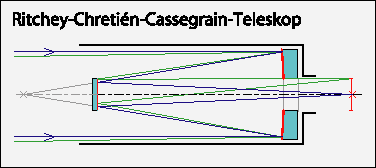
\includegraphics[scale=2]{rc_telescope.pdf}
  \caption[Strahlengang eines Ritchey-Chrétien Teleskops]{Strahlengang eines Ritchey-Chrétien Teleskops mit Fokusebene\cite{rc_telescope}.}
\end{figure}

Analog zum Cassegrain-Teleskop werden die Krümmungsradien der beiden Spiegel wie folgt berechnet:

\begin{align}
	R_1 &= \frac{2DF}{F-B}\\
    R_2 &= \frac{2DB}{F-B-D}
\end{align}
wobei
\begin{itemize}
	\item $F$ die effektive Brennweite des Gesamtsystems,
    \item $B$ der Abstand vom Sekundärspiegel zum Brennpunkt
    \item und $D$ der Abstand der beiden Spiegel ist.
\end{itemize}
Die konischen Konstanten werden dann so gewählt, dass sphärische Aberrationen und Komafehler dritter Ordnung eliminiert werden. Es ergibt sich\cite[S. 508-510]{optical_engineering}

\begin{align}
	K_1 &= -1-\frac{2}{M^3}\cdot\frac{B}{D}\\
    K_2 &= -1-\frac{2}{\left( M-1\right)^3}\left[ M\left( 2M-1\right) +\frac{B}{D}\right]
\end{align}
mit $M=F/f_1=(F-B)/D$ dem sekundären Abbildungsverhältnis. Für das Fraunhofer Teleskop sind diese Kennwerte $K_1=\num{-1.081}$ für den primären und $K_2=\num{-3.601}$ für den sekundären Spiegel\cite{fraunhofer}. Der Primärspiegel ist somit fast parabolisch, wohingegen der Sekundärspiegel hyperbolisch geformt ist. Zusätzlich kommt ein steuerbarer dritter Planspiegel als Fangspiegel zum Einsatz, der das Licht in eine von zwei Nasmyth-Fokusstationen ablenkt.\\
An einem dieser Ports ist eine Weitwinkelkamera (WWFI\cite{wwfi}) montiert, deren Gesichtsfeld etwa \SI{0.5}{\degree} des Himmels abbildet. Da das Bildfeld bei Teleskopen des Typs Ritchey-Chrétien im Allgemeinen nicht eben ist, wird an dem Port des WWFI eine dreilinsige Korrekturoptik eingesetzt, um eine flache Abbildung über \SI{0.7}{\degree} zu ermöglichen. WWFI besitzt ein Mosaik aus $2\times 2$ CCD-Sensoren mit insgesamt 64 Megapixel und ist das Instrument, welche die hier behandelten Fokusreihen aufnimmt.

\subsection{Fokussierung}

Da man es in der beobachtenden Astronomie stets mit praktisch unendlich weit entfernten Objekten zu tun hat, deren Entfernung sich somit auch nicht ändert, wäre es naheliegend, dass nur eine einzige Fokussierung nötig ist um das Teleskop zu eichen um mögliche Fertigungsabweichungen zu berücksichtigen. In der Realität wirken sich Veränderungen der Umgebungsbedingungen wie Verformung durch das Eigengewicht oder Wärmeausdehnung bei Temperaturänderung auf die Optik aus.\\

Für die Verschiebung des Fokus durch die Temperatur lässt sich folgende Überlegung anstellen. Der Längenausdehnungskoeffizient $\alpha$ eines Festkörpers der Länge $L$ ist definiert als die relative Längenänderung pro Temperaturänderung $\Delta T$.
\begin{align}
	\alpha &= \frac{\Delta L}{L\cdot \Delta T}
\end{align}
Für die temperaturabhängige Länge ergibt sich nach Integration
\begin{align}
	L(T) &= L(T_0)\cdot \exp[\int_{T_0}^T\alpha(T)\dd{t}].
\end{align}
Mit der Annahme, dass der Koeffizient nicht von der Temperatur abhängt, also $\alpha(T) = \alpha(T_0)$, lässt sich die Differentialgleichung gleich lösen.
\begin{align}
	L(T) &= \underbrace{L(T_0)}_{\equiv L_0}\cdot \exp[\alpha\cdot (\underbrace{T-T_0}_{\equiv \Delta T})]
\end{align}
Oder als Taylorentwicklung bis zur Ordnung $\mathcal{O}(\Delta T)$:
\begin{align}
	L &\approx L_0(1+\alpha\cdot\Delta T)\\
    \Rightarrow \Delta L &\approx \alpha \cdot L_0\cdot \Delta T
\end{align}
Die Fokusverschiebung durch die Temperaturänderung ist also für kleine $\Delta T$ in guter Näherung linear. Auf ähnliche Weise lässt sich argumentieren, dass die Verformung des Teleskops, die ja winkelabhängig von der Neigung des Teleskops ist, in erster Näherung zu einer linearen Stauchung und somit auch zu einer linearen Fokusverschiebung führt. Entsprechendes konnte für das Fraunhofer Teleskop in der Vergangenheit schon nachgewiesen werden\cite{commissioning}. Aufgrund der komplexen Geometrie des Teleskops und der verschiedenen Materialien ist es allerdings naheliegend, dass die wahre Funktion der Fokusverschiebung komplizierter ist.

\subsection{Aberrationen}

Die Zernike-Polynome bilden eine orthogonale Basis die verwendet werden kann um eine Wellenfront zu repräsentieren. Somit können Zernike-Polynome auch die Abbildungsfehler eines optischen Systems beschreiben.\\
Die Fokusserien, welche in dieser Arbeit behandelt werden, wurden bereits auf die Koeffizienten relevanter Zernike-Polynome reduziert. Dazu wurden für die Sterne in jeder Aufnahme mit der Donut Methode, wie beschrieben von Tokovinin und Heathcode 2006\cite{donut}, die Momente zweiter Ordnung berechnet.

\begin{mdframed}[style=emphasis]
\emph{Momente} in der Bildverarbeitung werden aus den gewichteten Mittelwerten der normierten Helligkeitswerte einzelner Pixel gebildet. Sie können dabei so gewählt werden, dass sie bestimmte Eigenschaften eines Bildes widerspiegeln oder gewisse geometrische Interpretationen besitzen. Insbesondere sind Momente hilfreich, um einzelne Objekte in einem segmentierten Bild zu beschreiben.
\end{mdframed}
Mit Hilfe der Momente werden folgende Koeffizienten definiert, die direkt proportional zu den entsprechenden Zernike Koeffizienten mit Noll-Indizes\cite{noll} sind.
\begin{align}
	A_4 &= p\sqrt{(M_x + M_y)/2}\\
    A_5 &= pM_{xy}(M_xM_y)^{-1/4}\\
    A_6 &= 0.5p(M_x-M_y)(M_xM_y)^{-1/4}
\end{align}
Dabei ist $p$ die Winkelausdehnung der Detektor Pixel. Diese Koeffizieten werden als Maß für Defokus ($A_4$) sowie schrägen und senkrechten Astigmatismus ($A_5, A_6$ resp.) verwendet.
\section{Statistische Grundlagen}
\subsection{B-Spline Interpolation}
Ein B-Spline der Ordnung $k$ wird gebildet, in dem man mehrere Polynome des Grads $k-1$, die maximal $C^{k-2}$ stetig an den Endpunkten sind, aneinanderhängt. Dabei definiert der aufsteigende Satz der Endpunkte $t_0 \le t_1 \le \ldots \le t_m$ den sog. Knotenvektor
\begin{align*}
	\va{T} = (t_0,t_1,\ldots,t_m),
\end{align*}
der die Parametrisierung der Basisfunktionen festlegt. Die Definition der Basisfunktionen, die sich als besonders numerisches stabil herausgestellt hat, ist wie folgt\cite{b-splines}:
\begin{align}
	N_{i,1}(t) &= \begin{cases}1 \text{ für } t_i \le t \le t_{i+1}\\0\text{ sonst}\end{cases}\\
    N_{i,k}(t) &= \frac{t-t_i}{t_{i+k-1}-t_i}N_{i,k-1}(t)+\frac{t_{i+k}-t}{t_{i+k}-t_{i+1}}N_{i+1,k-1}(t)\label{bspline}
\end{align}
für $i=0,1,\ldots,n$. Gleichung \eqref{bspline} gilt dabei für $k > 1$.\\
Eine B-Spline Kurve lässt sich dann schreiben als eine Linearkombination von Kontrollpunkten $\vb{p}_i$ und Basisfunktionen:
\begin{align}
	r(t) &= \sum_{i=0}^n\vb{p}_i N_{i,k}(t),\qquad n\ge k-1,\qquad t\in [t_{k-1},t_{n+1}].
\end{align}
Eine Parametrisierung der Form $f(x, y)=z$ lässt sich nun mit Hilfe einer B-Spline Fläche interpolieren. Die B-Spline Fläche ist das Tensorprodukt zweier B-Splines und wird daher definiert durch einen rechteckigen Satz an Kontrollpunkten $\vb{p}_{ij},0\le i\le m, 0\le j \le n$ und zwei Knotenvektoren $\va{X} = (x_0,x_1,\ldots,x_{m+k})$ und $\va{Y} = (y_0,y_1,\ldots,y_{n+l})$ entsprechend der veränderlichen $x$ und $y$.
Die Fläche ist dann gegeben durch
\begin{align}
	f^*(x, y) = \sum_{i=0}^m\sum_{j=0}^n \vb{p}_{ij} N_{i,k}(x)N_{j,l}(y).
\end{align}
Die nötigen Kontrollpunkte können mit einem QuickHull Algorithmus bestimmt werden\cite{surface}. Insbesondere sind die Kontrollpunkte im Gegensatz zu Bézierkurven nicht notwendigerweise Teil des Interpolanten. Durch Wiederholen eines Punktes im Knotenvektor kann die Differenzierbarkeit des Interpolanten an diesem Punkt um jeweils $1$ heruntergesetzt werden. Ein Knotenpunkt der Multiplizität $k$ für ein B-Spline $k$-ter Ordnung zwingt den Interpolanten somit den Wert des Knotenpunkts an der entsprechenden Stelle anzunehmen.\\
Eine so bestimmte Interpolations-Fläche nimmt zwar an den Eckpunkten garantiert die Werte der Knotenvektoren ein, ist allerdings auch nur innerhalb der von den Knotenvektoren aufgespannten konvexen Hülle definiert. Möchte man, dass dieser Interpolant auch Werte für Regionen außerhalb seiner konvexen Hülle liefert, müssen diese extrapoliert werden.
\subsection{Korrelation und Transinformation}
Die Korrelation beschreibt den statistischen Zusammenhang zweier Ereignisse. Dieser Zusammenhang muss dabei nicht notwendigerweise auf eine kausale Beziehung zurückzuführen sein und kann rein stochastischer Natur sein.\\
Im Rahmen dieser Arbeit wird die Korrelation diskreter Wahrscheinlichkeitsverteilungen untersucht. Das Mittel der Wahl stellt die Transinformation (auch engl. \emph{mutual information}) dar. Sie ist ein Maß für die Korrelation der Distributionen, welche im Vergleich zum Korrelationskoeffizienten nicht nur lineare sondern auch nicht-lineare Abhängigkeiten berücksichtigt\cite{mi_corr}.\\
Die Transinformation kann auch als Wert interpretiert werden, der angibt wie sehr die multivariate Verteilung $p(X, Y)$ dem Produkt der Verteilungen $p(X) p(Y)$ ähnelt. Formal kann sie dann definiert werden als:
\begin{align}
	I(X,Y) &= \sum_{y\in Y}\sum_{x\in X}p(x,y)\log(\frac{p(x,y)}{p(x)p(y)})
\end{align}
mit der multivariaten Wahrscheinlichkeitsdichtefunktion $p(x, y)$ der Mengen $X$ und $Y$ sowie $p(x)$ und $p(y)$ den Randverteilungen von $X$ und $Y$ respektive. Handelt es sich um unabhängige Verteilungen, so faktorisiert $p(x, y)$ und der Transinformationsgehalt ist folglich $\num{0}$, da für den Logarithmus gilt:
\begin{align}
	\log(\frac{p(x)p(y)}{p(x)p(y)}) = \log(1) = 0.
\end{align}
Im weiteren kann die Transinformation noch normiert werden, wenn man sie als Kovarianz und die Shannon-Entropie analog als Varianz interpretiert\cite{mi_norm}:
\begin{align}
	I_{\mathrm{norm}}(X,Y) &= \frac{I(X,Y)}{\sqrt{H(X)H(Y)}}
\end{align}
mit $H(X)$ und $H(Y)$ der Shannon-Entropie der jeweiligen Verteilungsfunktion.
  \chapter{Datenreduktion der Fokusserien}
\label{chapter_2}
Die in diesem Kapitel beschriebenen Schritte wurden in kleinen Programmen mithilfe der Programmiersprache Python implementiert. Eine ausgiebige Dokumentation der Funktionen sowie deren Gebrauch findet sich im Softwarerepositorium gemeinsam mit dem Quelltext.\\
An dieser Stelle sollen die von den Programmen erstellten Plots nur exemplarisch präsentiert werden, um die Übersichtlichkeit nicht zu beeinträchtigen. Im Anhang findet sich eine vollständige Übersicht aller Parameter und ihrer Plots.

\section{Diskrete Dichteverteilungsfunktionen}
In einem ersten Schritt wurden die Daten der Fokusserien aufbereitet um diskrete Verteilungsfunktionen zu erhalten. Für jede Aufnahme stand ein Satz an Teleskop-spezifischen Meta-Parametern (TSI-Parameter) sowie eine Liste aller Sterne und ihre Pixel-Position sowie Abberations-Koeffizieten (PSF-Parameter), wie in Kapitel 1 beschrieben, zur Verfügung.\\
Die PSF-Parameter wurden für jede Aufnahme auf ihren Median reduziert. Um dennoch womögliche Unterschiede in der Position auf dem Detektor-Mosaik feststellen zu können, wird jede Aufnahme in ein $3\times 3$ aufgeteilt und jedem Quadrat im Gitter der Median der jeweiligen Sterne im Quadrat zugeteilt. Das Ergebnis sind Verteilungsfunktionen aller PSF-Parameter für 9 quadratische Bildbereiche auf dem Detektor (Abb. \ref{a4_dist}).\\
Für die Distributionen der TSI-Parameter war keine weitere Reduktion nötig (Abb. \ref{tsi_temp}). Allerdings wurden aufgrund der hohen Anzahl der Parameter statische und quasi-statische Parameter entfernt. Als quasi-statisch wurden solche Parameter interpretiert, deren Werte bei einem Binning von 50 zu $\ge\SI{95}{\percent}$ auf einen Wert fallen.
\vfill\,

\begin{figure}[H]
	\centering
	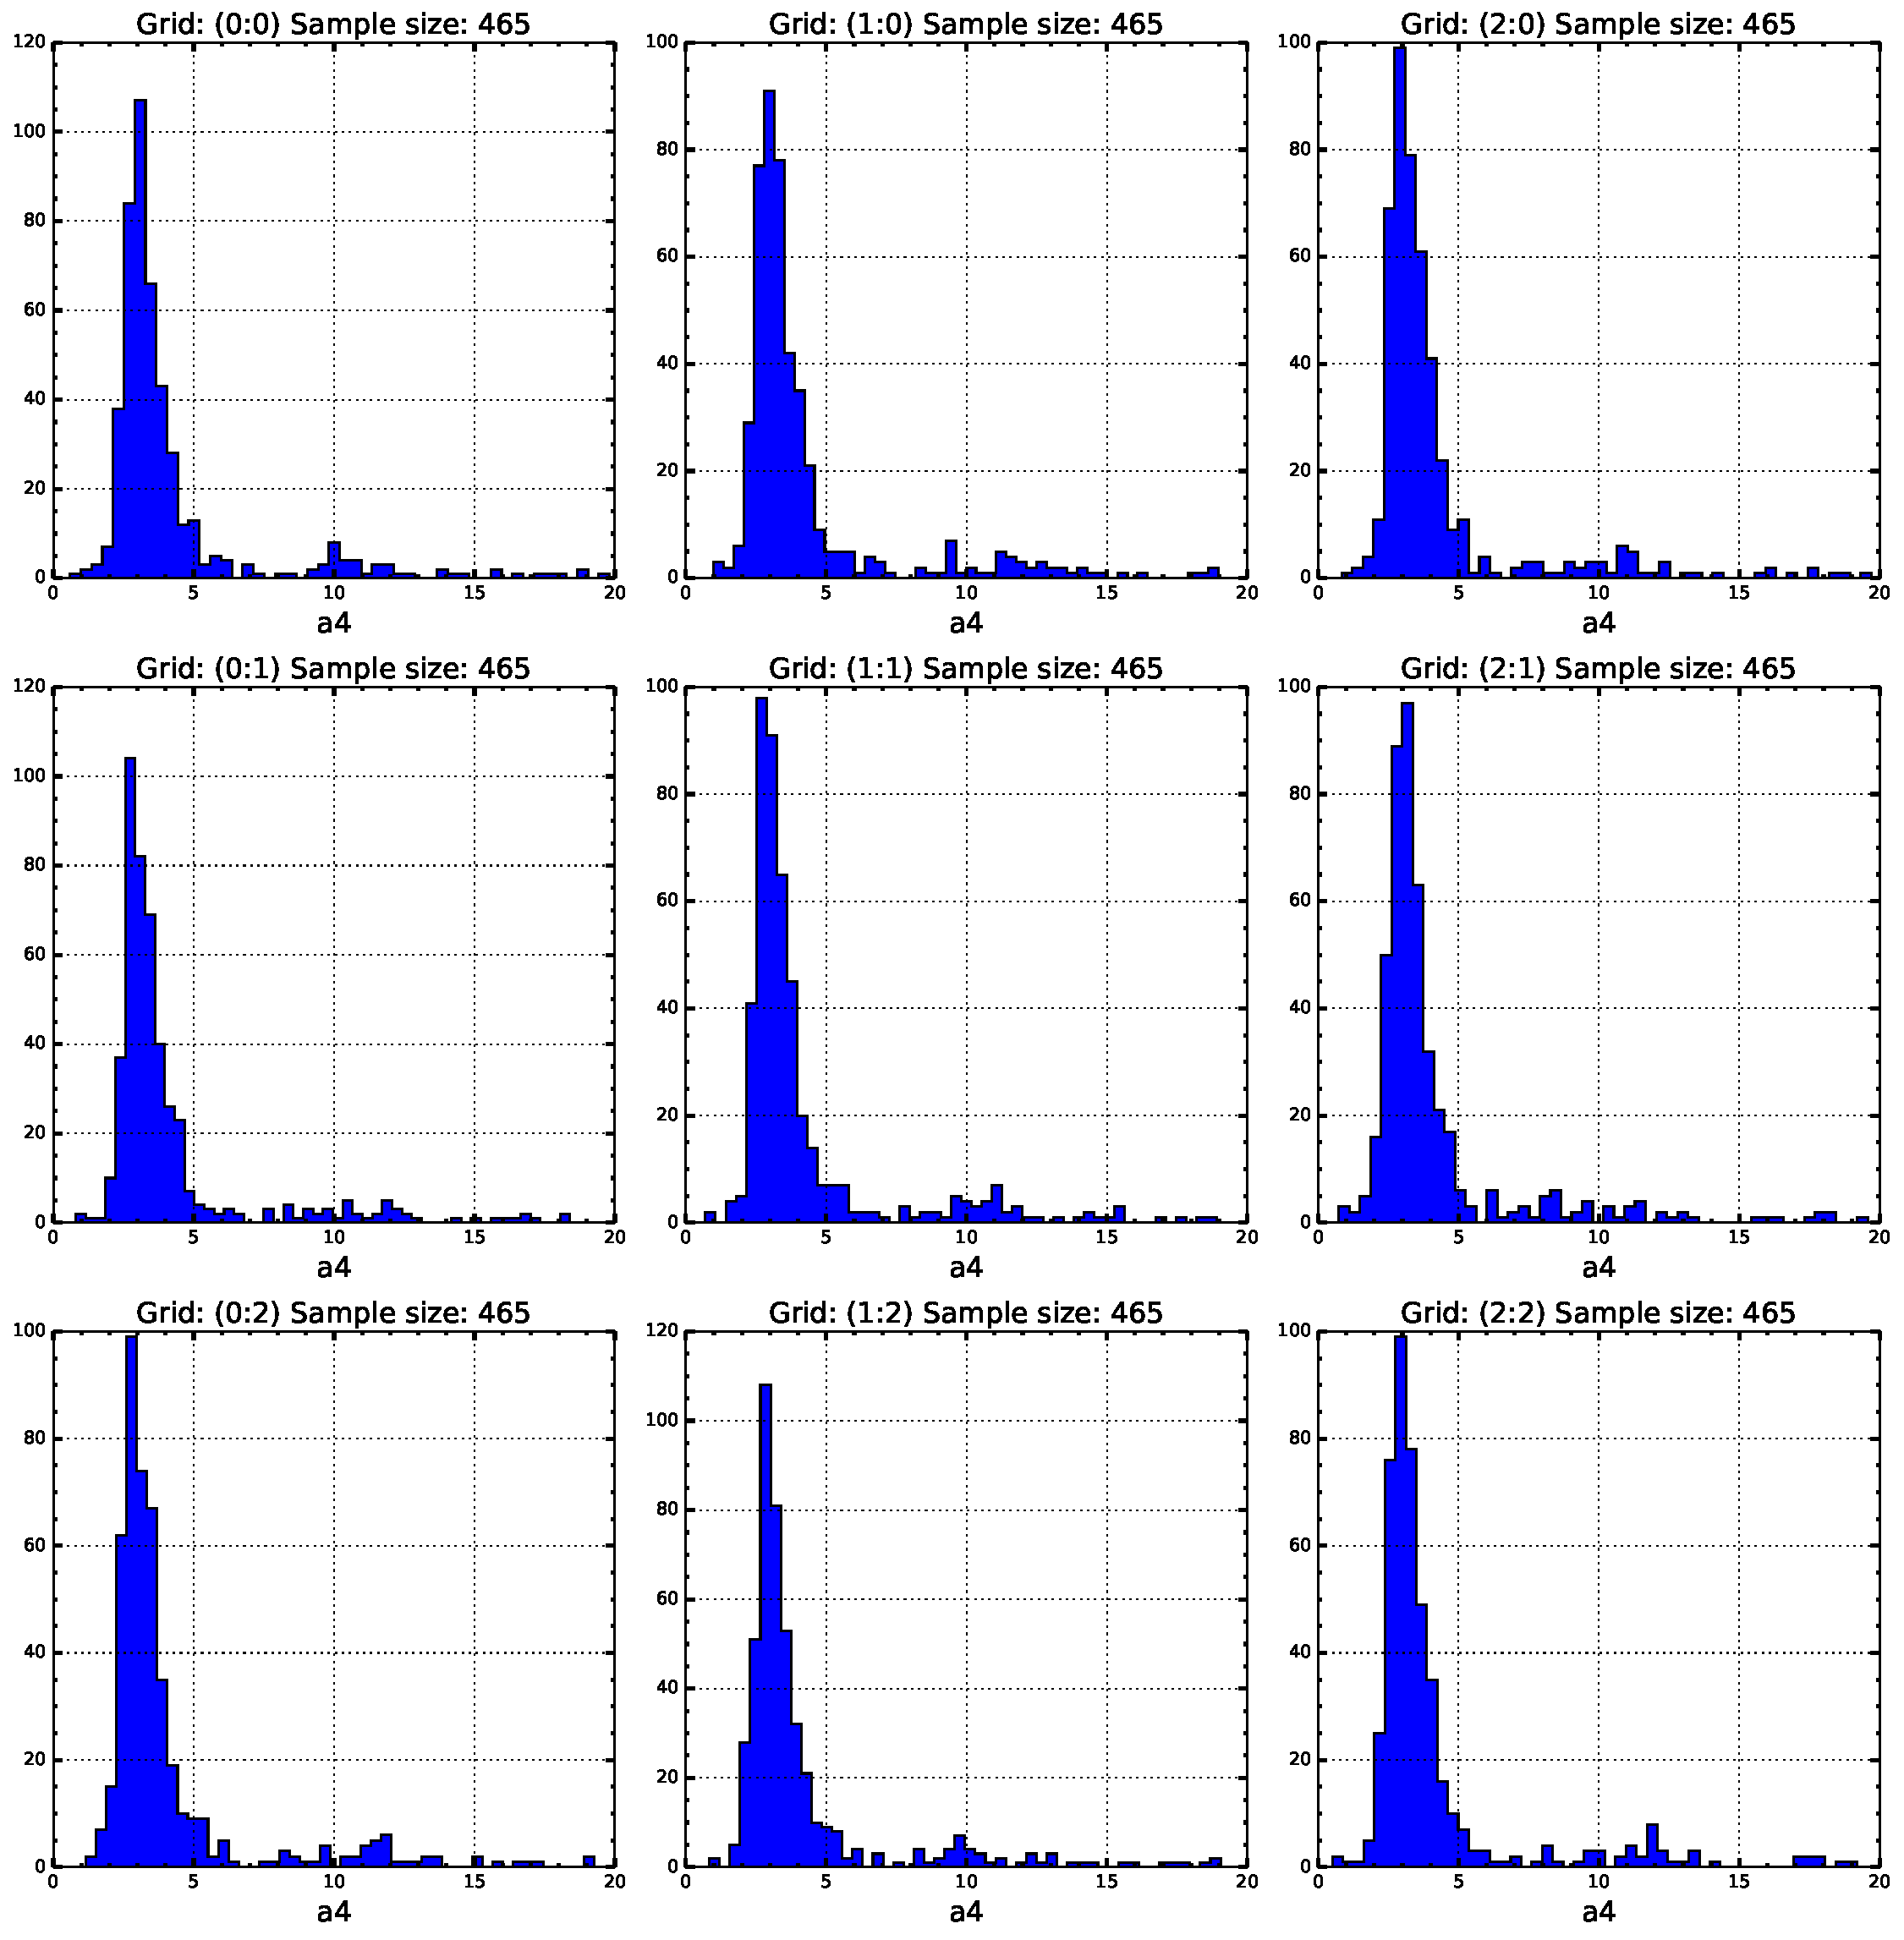
\includegraphics[scale=.40]{psf_dist/a4.pdf}
	\caption[Diskrete Verteilungsfunktionen des PSF-Parameters $A_4$]{Diskrete Verteilungsfunktionen des PSF-Parameters $A_4$. Die Lage des Plots in der Grafik entspricht der Gitter-Position des Quadrats auf dem Detektor. Zugrunde liegen die Daten der ausgewählten Fokus-Aufnahmen aus 465 Fokusserien. Für den Plot wurde der Definitionsbereich in 50 gleichgroße Teilstücke geteilt und die Werte in den Teilstücken gezählt (sog. \emph{Binning}).}
    \label{a4_dist}
\end{figure}

\begin{figure}[H]
	\centering
	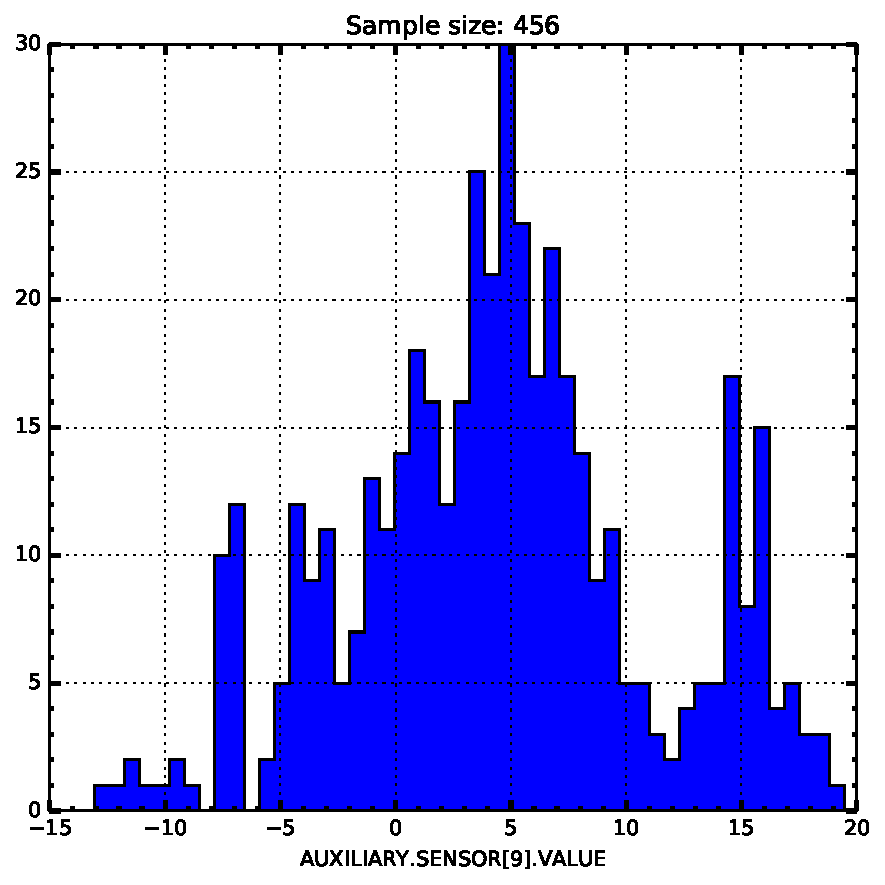
\includegraphics[scale=.75]{tsi_dist/AUXILIARY_SENSOR_9__VALUE.pdf}
	\caption[Diskrete Verteilungsfunktion eines Temperatursensors]{Diskrete Verteilungsfunktion eines Temperatursensors. Zugrunde liegen die Daten der ausgewählten Fokus-Aufnahmen aus 456 Fokusserien. Binning: 50.}
    \label{tsi_temp}
\end{figure}

\section{Transinformation der Aberrations-Koeffizieten sowie der Teleskop Meta-Daten}

Um zu überprüfen ob es weitere Abhängigkeiten im Teleskop-System gibt, die sich auf den Fokus auswirken, wurden alle Verteilungsfunktionen (sowohl PSF- als auch TSI-Parameter) miteinander verglichen und ein normierter Transinformations-Index berechnet.\\
Diese Information liegt zunächst tabelliert vor. Damit sie effektiv betrachtet und analysiert werden kann, wurde sie in eine Korrelationsmatrix eingetragen und in einem Heatmap-Diagramm geplottet (Abb. \ref{psf_heatmap}).

\begin{figure}[H]
	\centering
	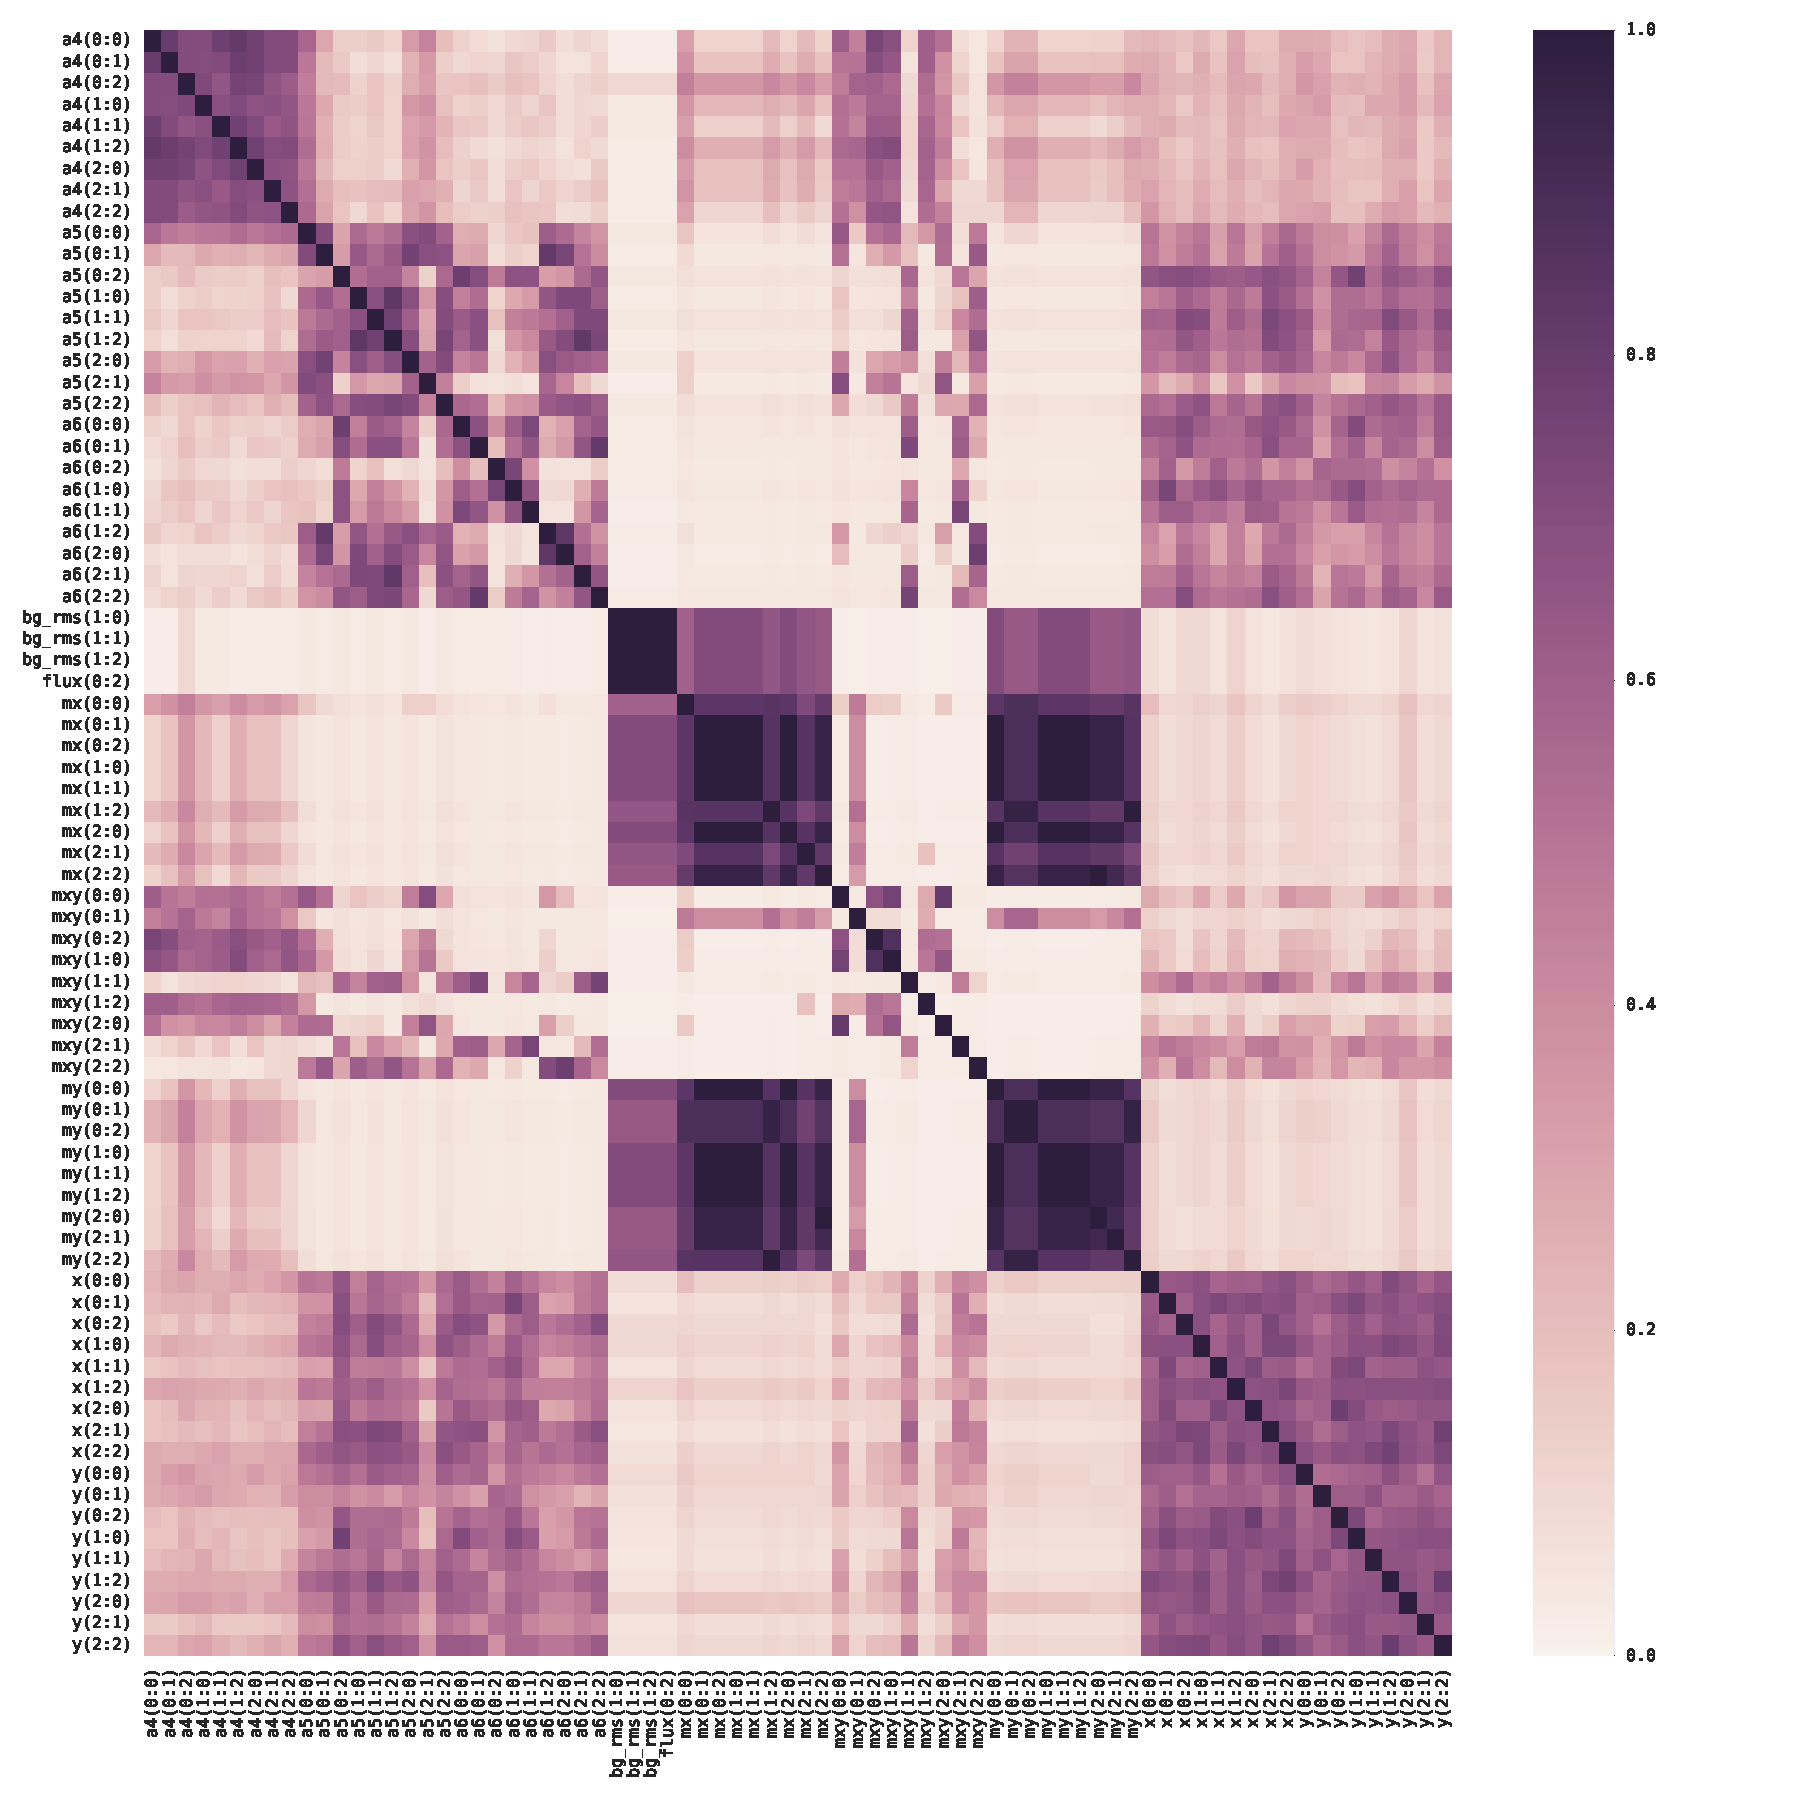
\includegraphics[scale=.56]{heatmaps/psf.pdf}
	\caption[Transinformations-Heatmap der PSF-Parameter]{Transinformations-Heatmap der PSF-Parameter. Jeder Pixel auf der Karte entspricht einem normierten Transinformations-Index. Da beide Achsen die selben Parameter enthalten nimmt jeder Wert auf der Diagonalen den Wert $\num{1}$ an.}
    \label{psf_heatmap}
\end{figure}

\section{Einfluss der Windgeschwindigkeit und Windrichtung}
Vor dem Bau des Fraunhofer Teleskops konnten bereits gute Beobachtungsbedingungen, insbesondere Seeing, am Wendelstein Observatorium nachgewiesen werden\cite{wendelstein_seeing}. Dennoch wurde ein Werkzeug entwickelt, um den Zusammenhang zwischen schlechter Bildqualität und Windgeschwindigkeit sowie Windrichtung auswerten zu können. Hierzu wurden aus den meteologischen Logdateien für jede Fokusaufnahme die relevanten Windwerte extrahiert und mit den PSF-Mittelwerten der Aufnahme verknüpft. Somit lassen sich die PSF-Parameter in Abhängigkeit von Windgeschwindigkeit, Windrichtung und Temperatur darstellen und auf mögliche Muster überprüfen (Abb. \ref{wind_a4}).

\begin{figure}[h]
	\centering
	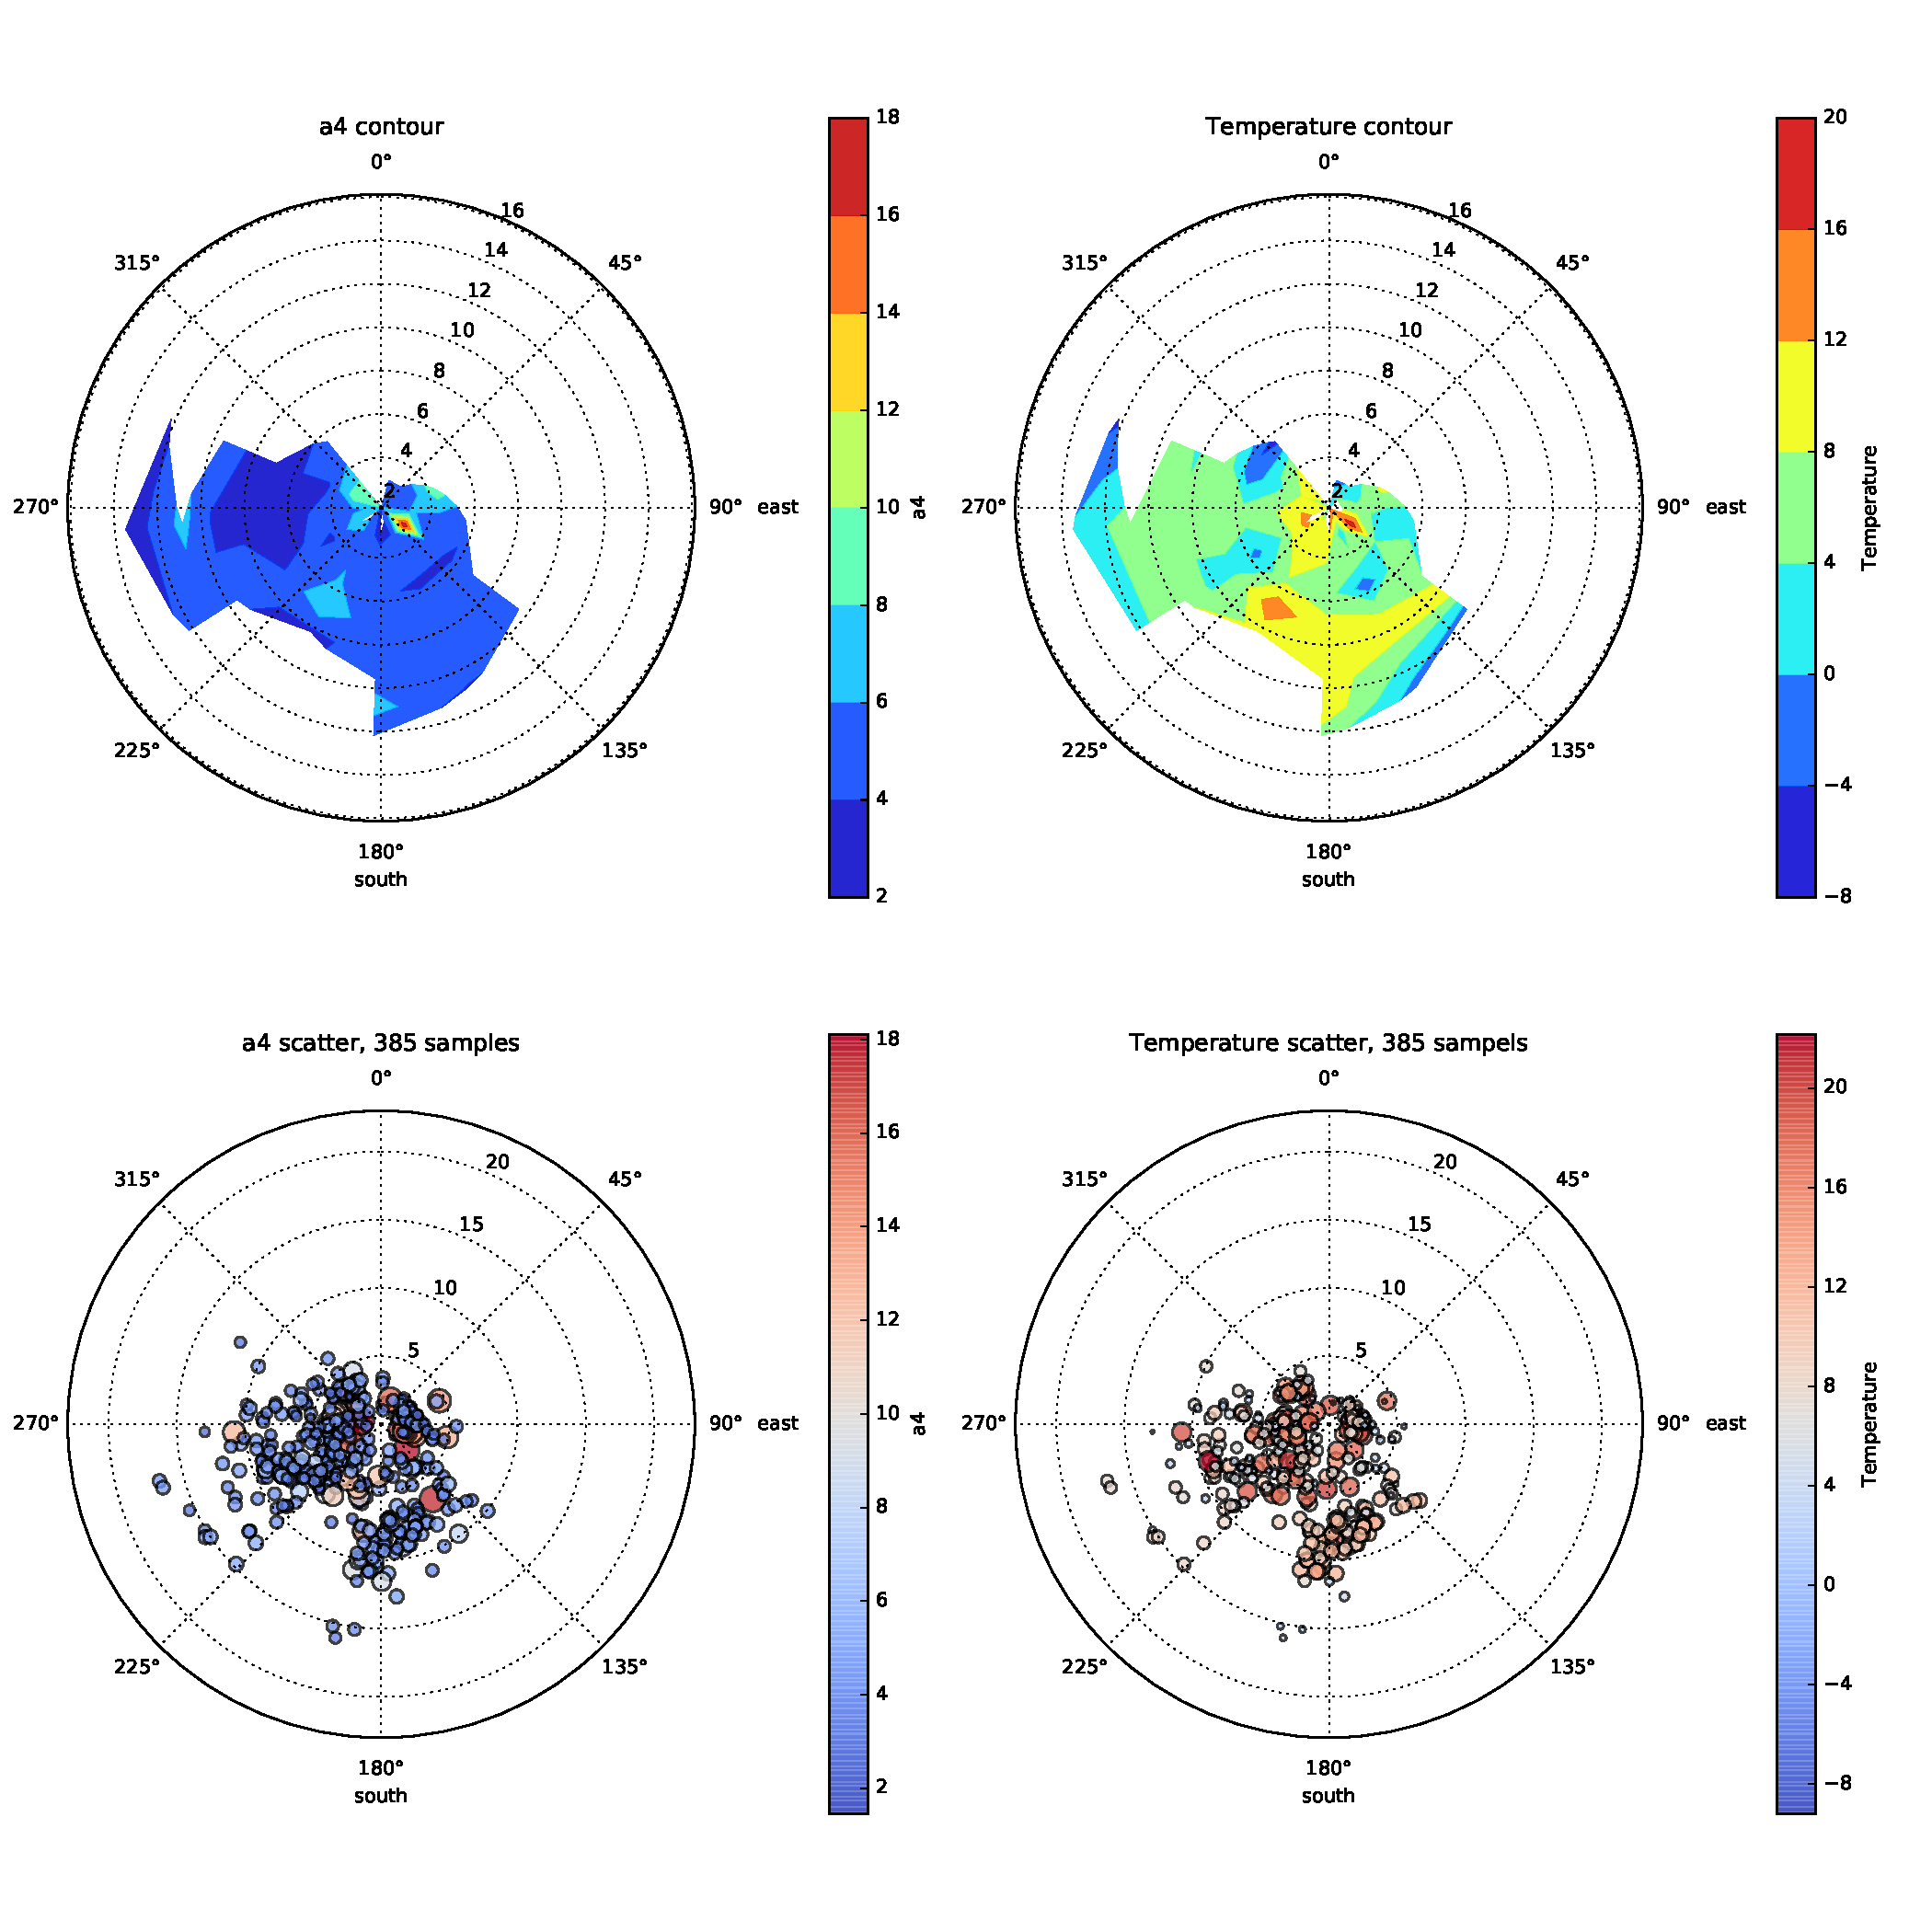
\includegraphics[scale=.48]{wind/wind_a4.pdf}
	\caption[Einfluss von Windgeschwindigkeit und Windrichtung auf $A_4$]{Einfluss von Windgeschwindigkeit und Windrichtung auf $A_4$. Die Plots in der linken Spalte zeigen $A_4$ gemäß der Farbskala an. Im unteren Plot ist die Größe der Kreise zusätzlich proportional zu $A_4$. Jeder Kreis repräsentiert eine von 385 Fokusaufnahmen. Analog stellt die rechte Spalte die Temperatur dar. Die Position in Polarkoordinaten wird durch den Wind bestimmt. Der Winkel entspricht der Windrichtung, der Abstand vom Nullpunkt entspricht der Windstärke in \si{\metre\per\second}.}
    \label{wind_a4}
\end{figure}

\section{Temperatur- und Elevationsabhängigkeit}

Im Rahmen dieser Arbeit wurden zwar Methoden entwickelt, um den Fokus des Teleskops auf weitere Abhängigkeiten hin zu überprüfen, die Herleitung einer neuen Fokusfunktion jedoch hat sich auf die Temperatur- und Elevationsabhängigkeit konzentriert.\\
In einem ersten Schritt wurden dazu die PSF-Parameter in Abhängigkeit von Temperatur und Elevation dargestellt. Die Punkte der diskreten Verteilungsfunktionen wurde auf ein Temperatur-Elevations-Gitter weniger Punkte reduziert, welche als Kontrollpunkte für einen B-Spline Flächeninterpolanten dienen. Bei der Reduktion werden alle Punkte innerhalb eines regelmäßigen Temperatur-Elevations-Quadrats herangezogen um einen Mittelwert zu berechnen. Dieser Mittelwert kann der Durchschnitt, Median, die Standardabweichung oder Varianz sein und ist mit einem Fehler versehen. Die jeweils verwendete Methode kann aus dem Titel des Plots abgelesen werden (Abb. \ref{a4_surf}).\\
Mit dem gleichen Verfahren wurde auch die Temperatur- und Elevationsabhängigkeit der Spiegel-Position auf der optischen Achse dargestellt. Hier fließen jeweils nur die besten Aufnahmen der Fokusserie mit ein. Dies sind folglich die Einstellungen, die schließlich für die Science-Aufnahmen verwendet wurden. Der so ermittelte Interpolant ist bereits ein guter Kandidat für eine neue Fokusfunktion.

\begin{figure}[h]
	\centering
	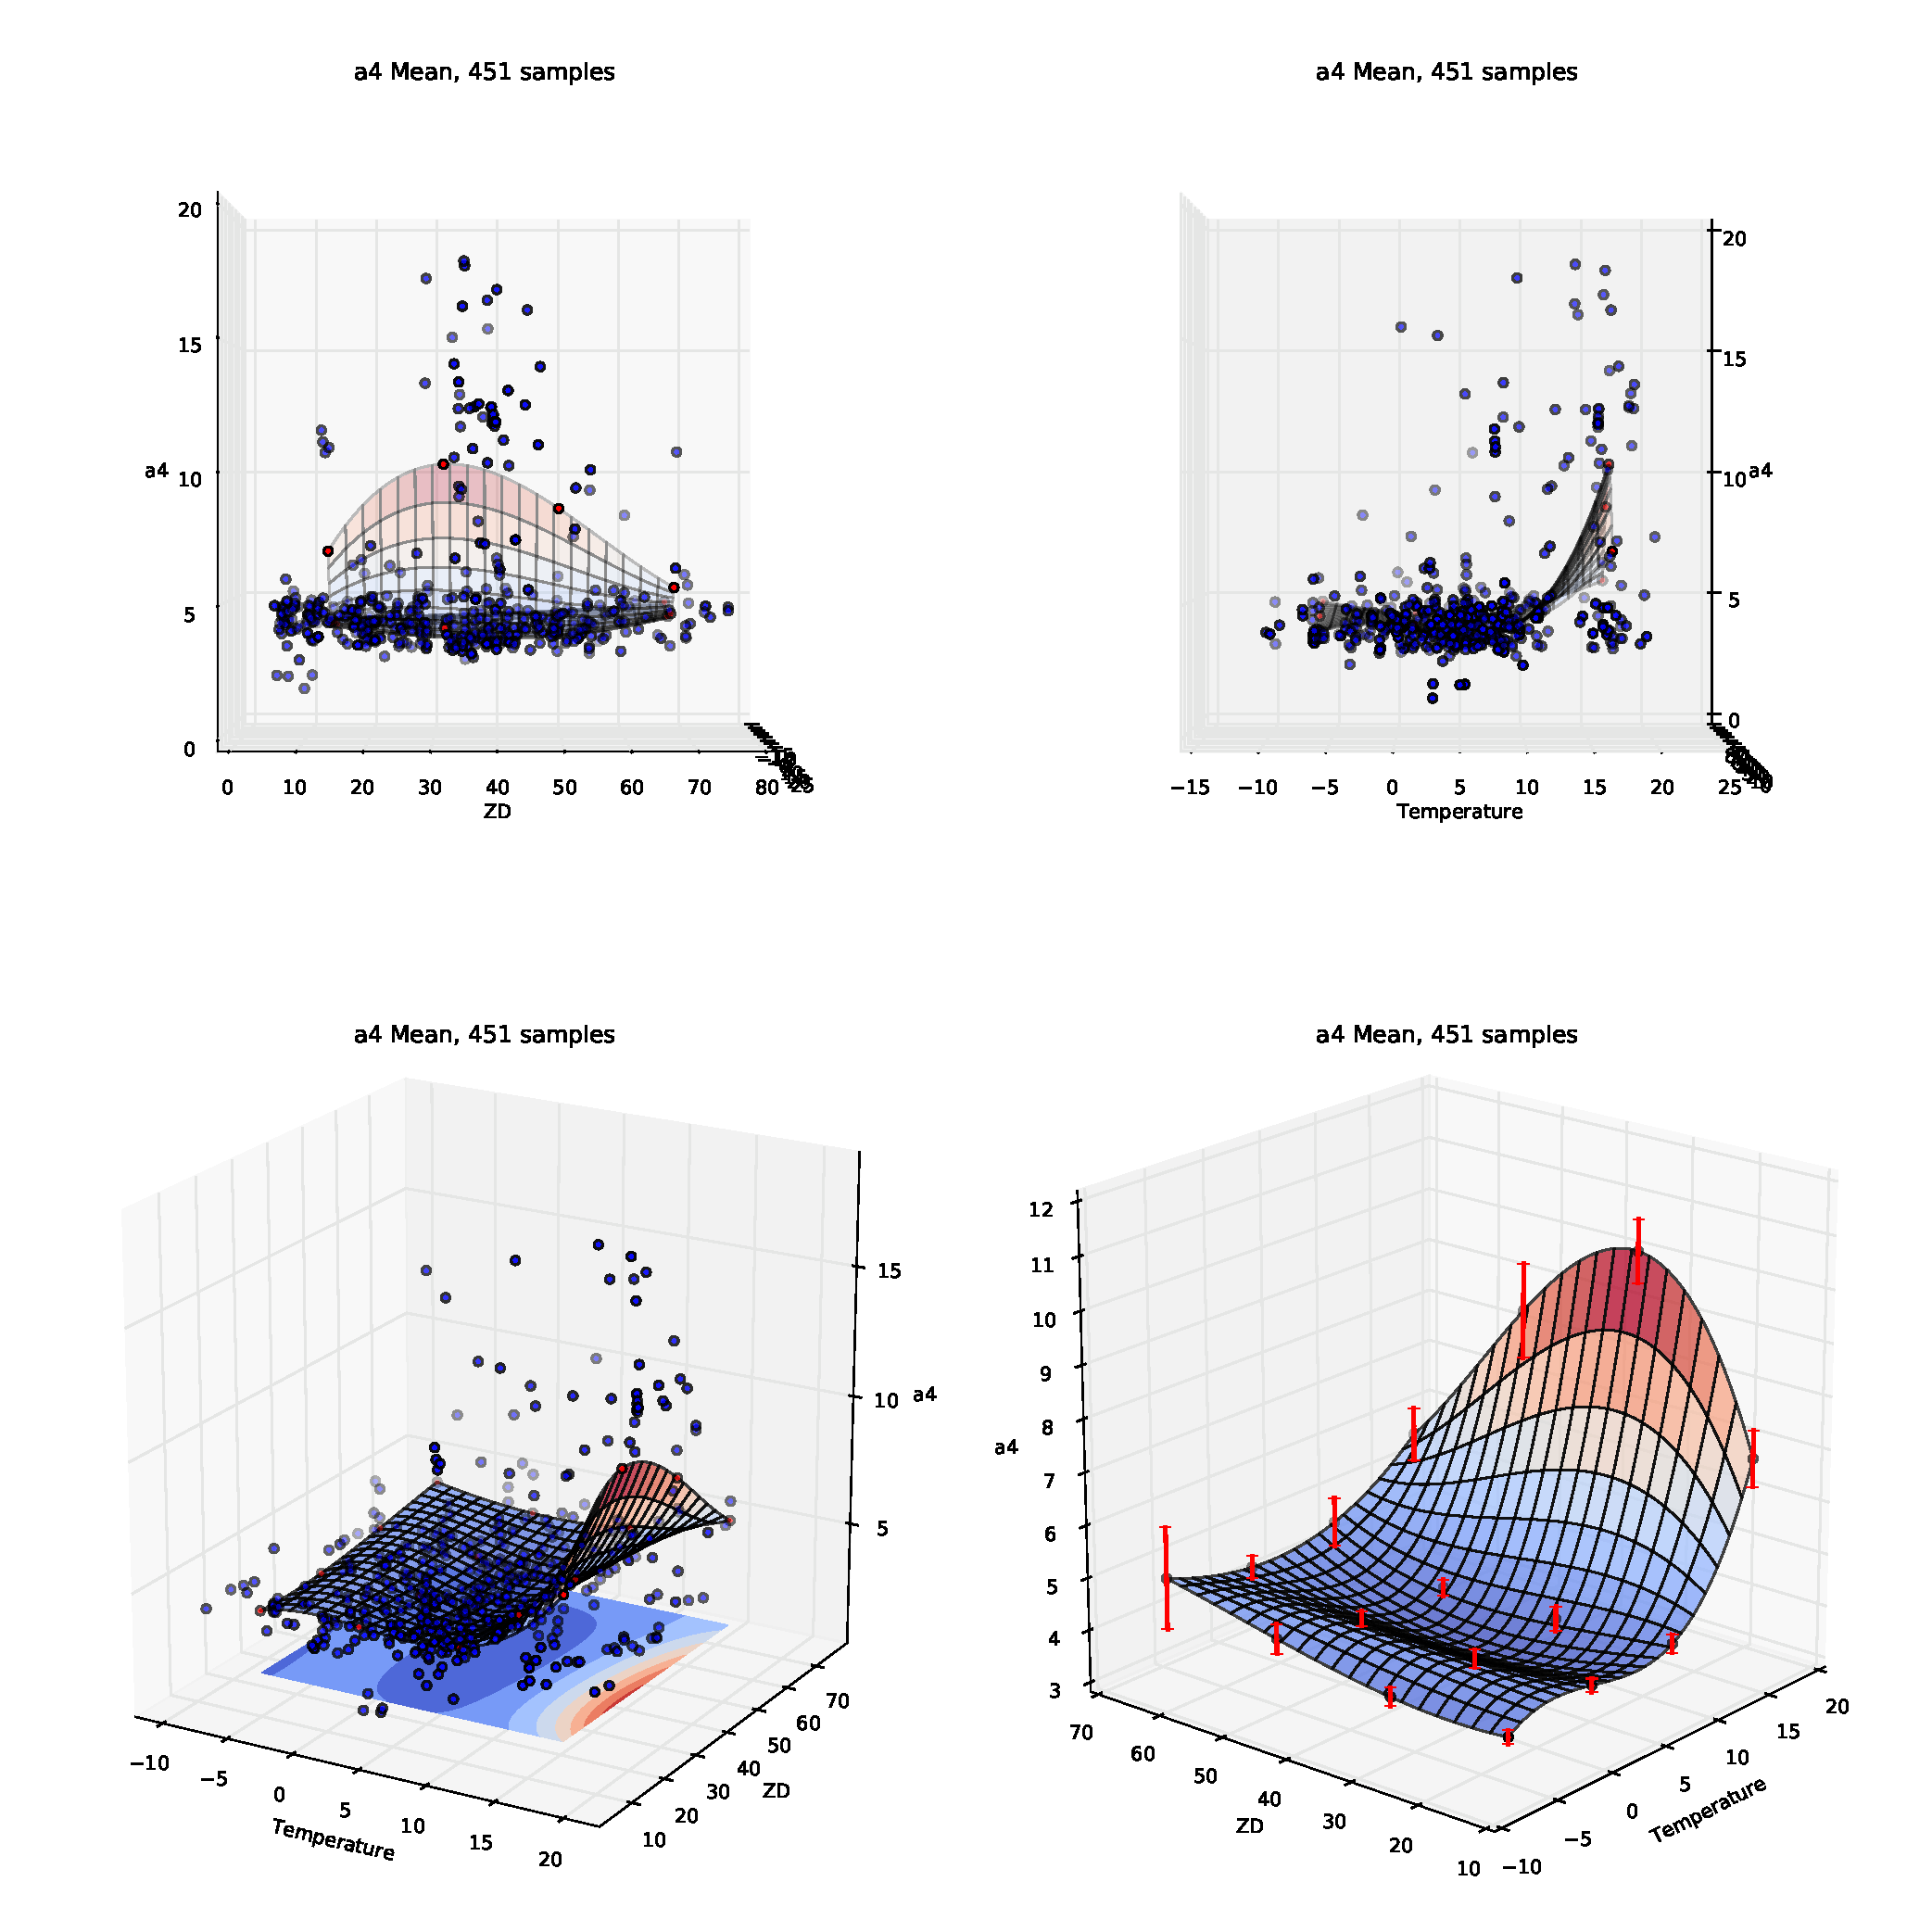
\includegraphics[scale=.48]{psf_surf/a4_mean.pdf}
	\caption[Temperatur- und Elevationsabhängigkeit von $A_4$]{Temperatur- und Elevationsabhängigkeit von $A_4$. Es liegen 451 Fokusaufnahmen zugrunde, die jeweils einem blauen Punkt entsprechen. Die Plots oben links und rechts entsprechen der Projektion auf die Temperatur- und Elevations-Achse respektive. Die roten Kontrollpunkt wurden als Durchschnittswerte berechnet (mean). Die roten Balken an den Kontrollpunkten im Plot unten rechts sind ein Maß für die Streuung des Kontrollpunktes. }
    \label{a4_surf}
\end{figure}

\begin{figure}[h]
	\centering
	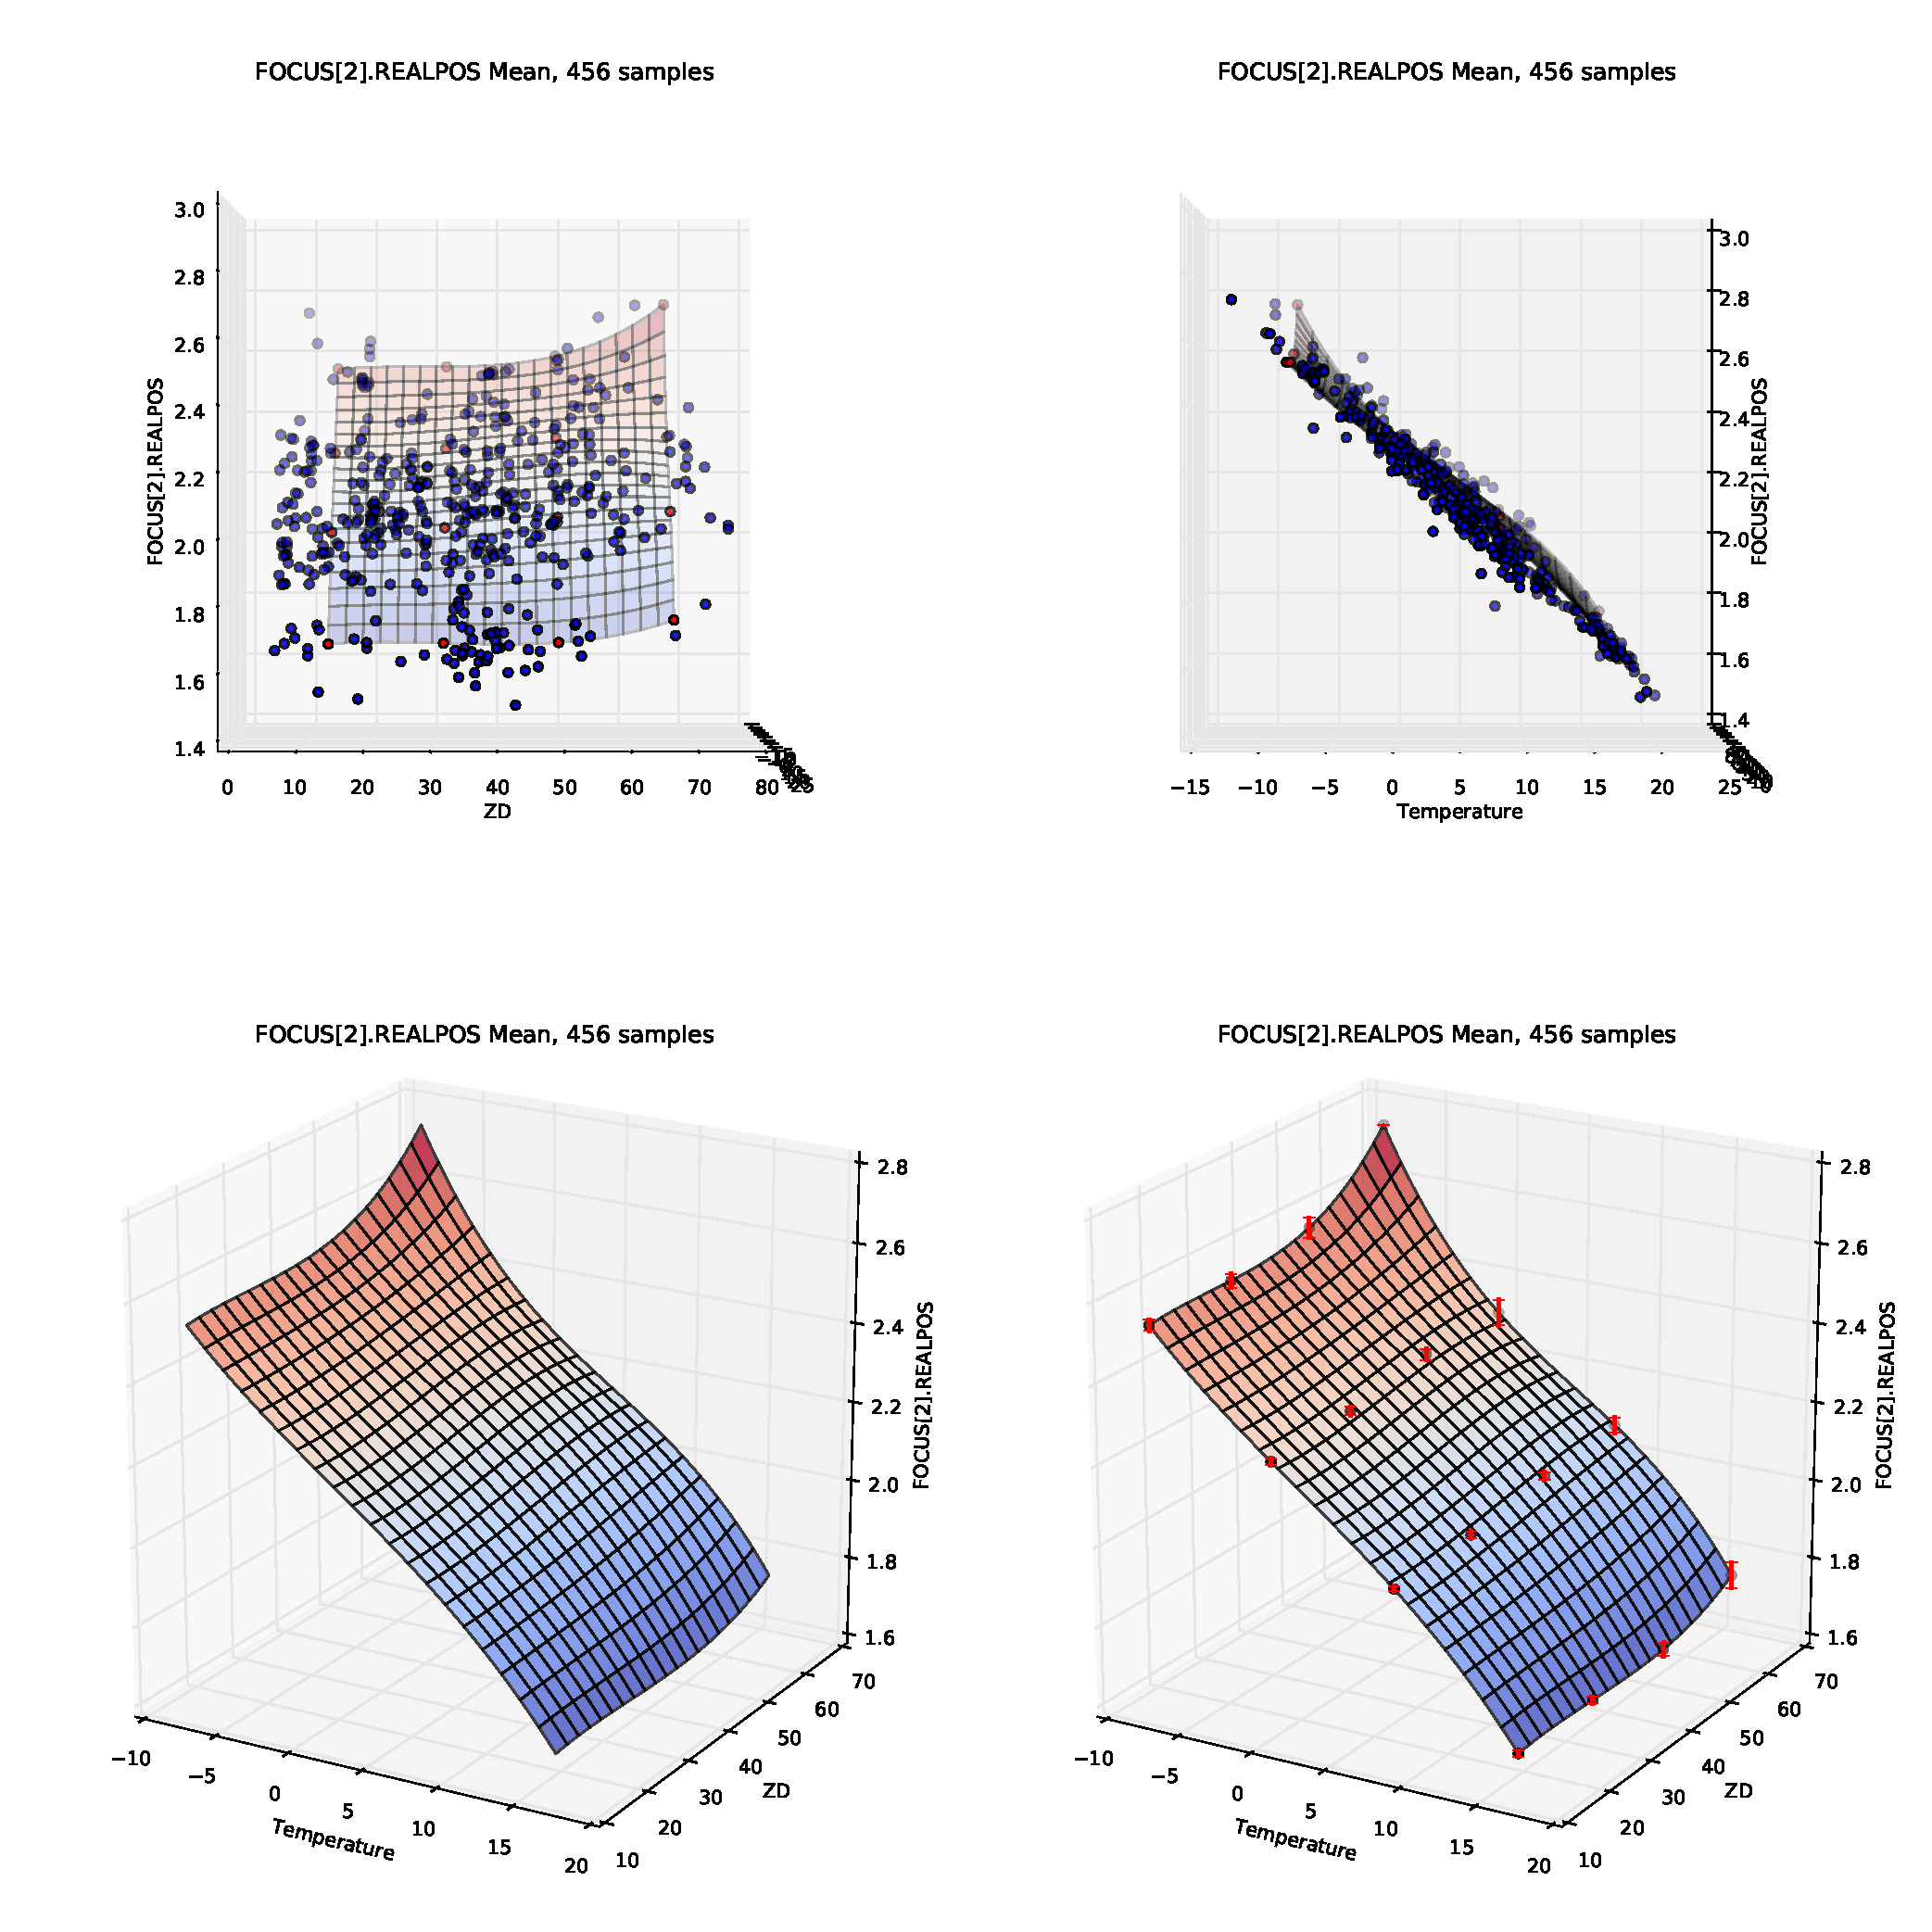
\includegraphics[scale=.45]{tsi_surf/POSITION_INSTRUMENTAL_FOCUS_2__REALPOS_mean.pdf}
	\caption[Temperatur- und Elevationsabhängigkeit der Sekundärspiegelposition]{Temperatur- und Elevationsabhängigkeit der Sekundärspiegelposition entlang der optischen Achse. Die Sekundärspiegelposition von 456 Fokusaufnahmen entsprechen den blauen Punkten. Die roten Kontrollpunkte im Plot unten rechts wurden über den Median aller Punkte in ihrer Umgebung gebildet und enthalten einen roten Fehlerbalken.}

    \label{focus_surf}
\end{figure}

  \chapter{Ergebnisse}

\section{Interpretation}
\subsection{Transinformation}
Die Transinformation ist ein nützliches Werkzeug, um in einem komplexen Parameterraum eine erste Orientierung zu bekommen. Da wir es in diesem Kontext mit zwei distinkten Sätzen an Parametern zu tun haben, wurden drei Korrelationsmatrizen geplottet: eine welche die Transinformation zwischen TSI-Parametern betrachtet, eine weitere für die PSF-Parameter und eine für Korrelationen zwischen PSF- und TSI-Parametern.\\
Die TSI- und PSF-Korrelationsmatrizen haben auf beiden Achsen dieselben Parameter. Eine Konsequenz daraus ist, dass die Matrizen sowohl symmetrisch sind, als auch den Transinformationswert 1 auf der Diagonalen besitzen, da eine Verteilung mit sich selbst völlig korreliert (Abb. \ref{heatmap_tsi_inline} und \ref{heatmap_psf_inline}). Entsprechend weist die PSF/TSI Matrix keines dieser beiden Merkmale auf (Abb. \ref{heatmap_psf_tsi_inline}).\\
\vfill\,

\begin{figure}[H]
	\centering
	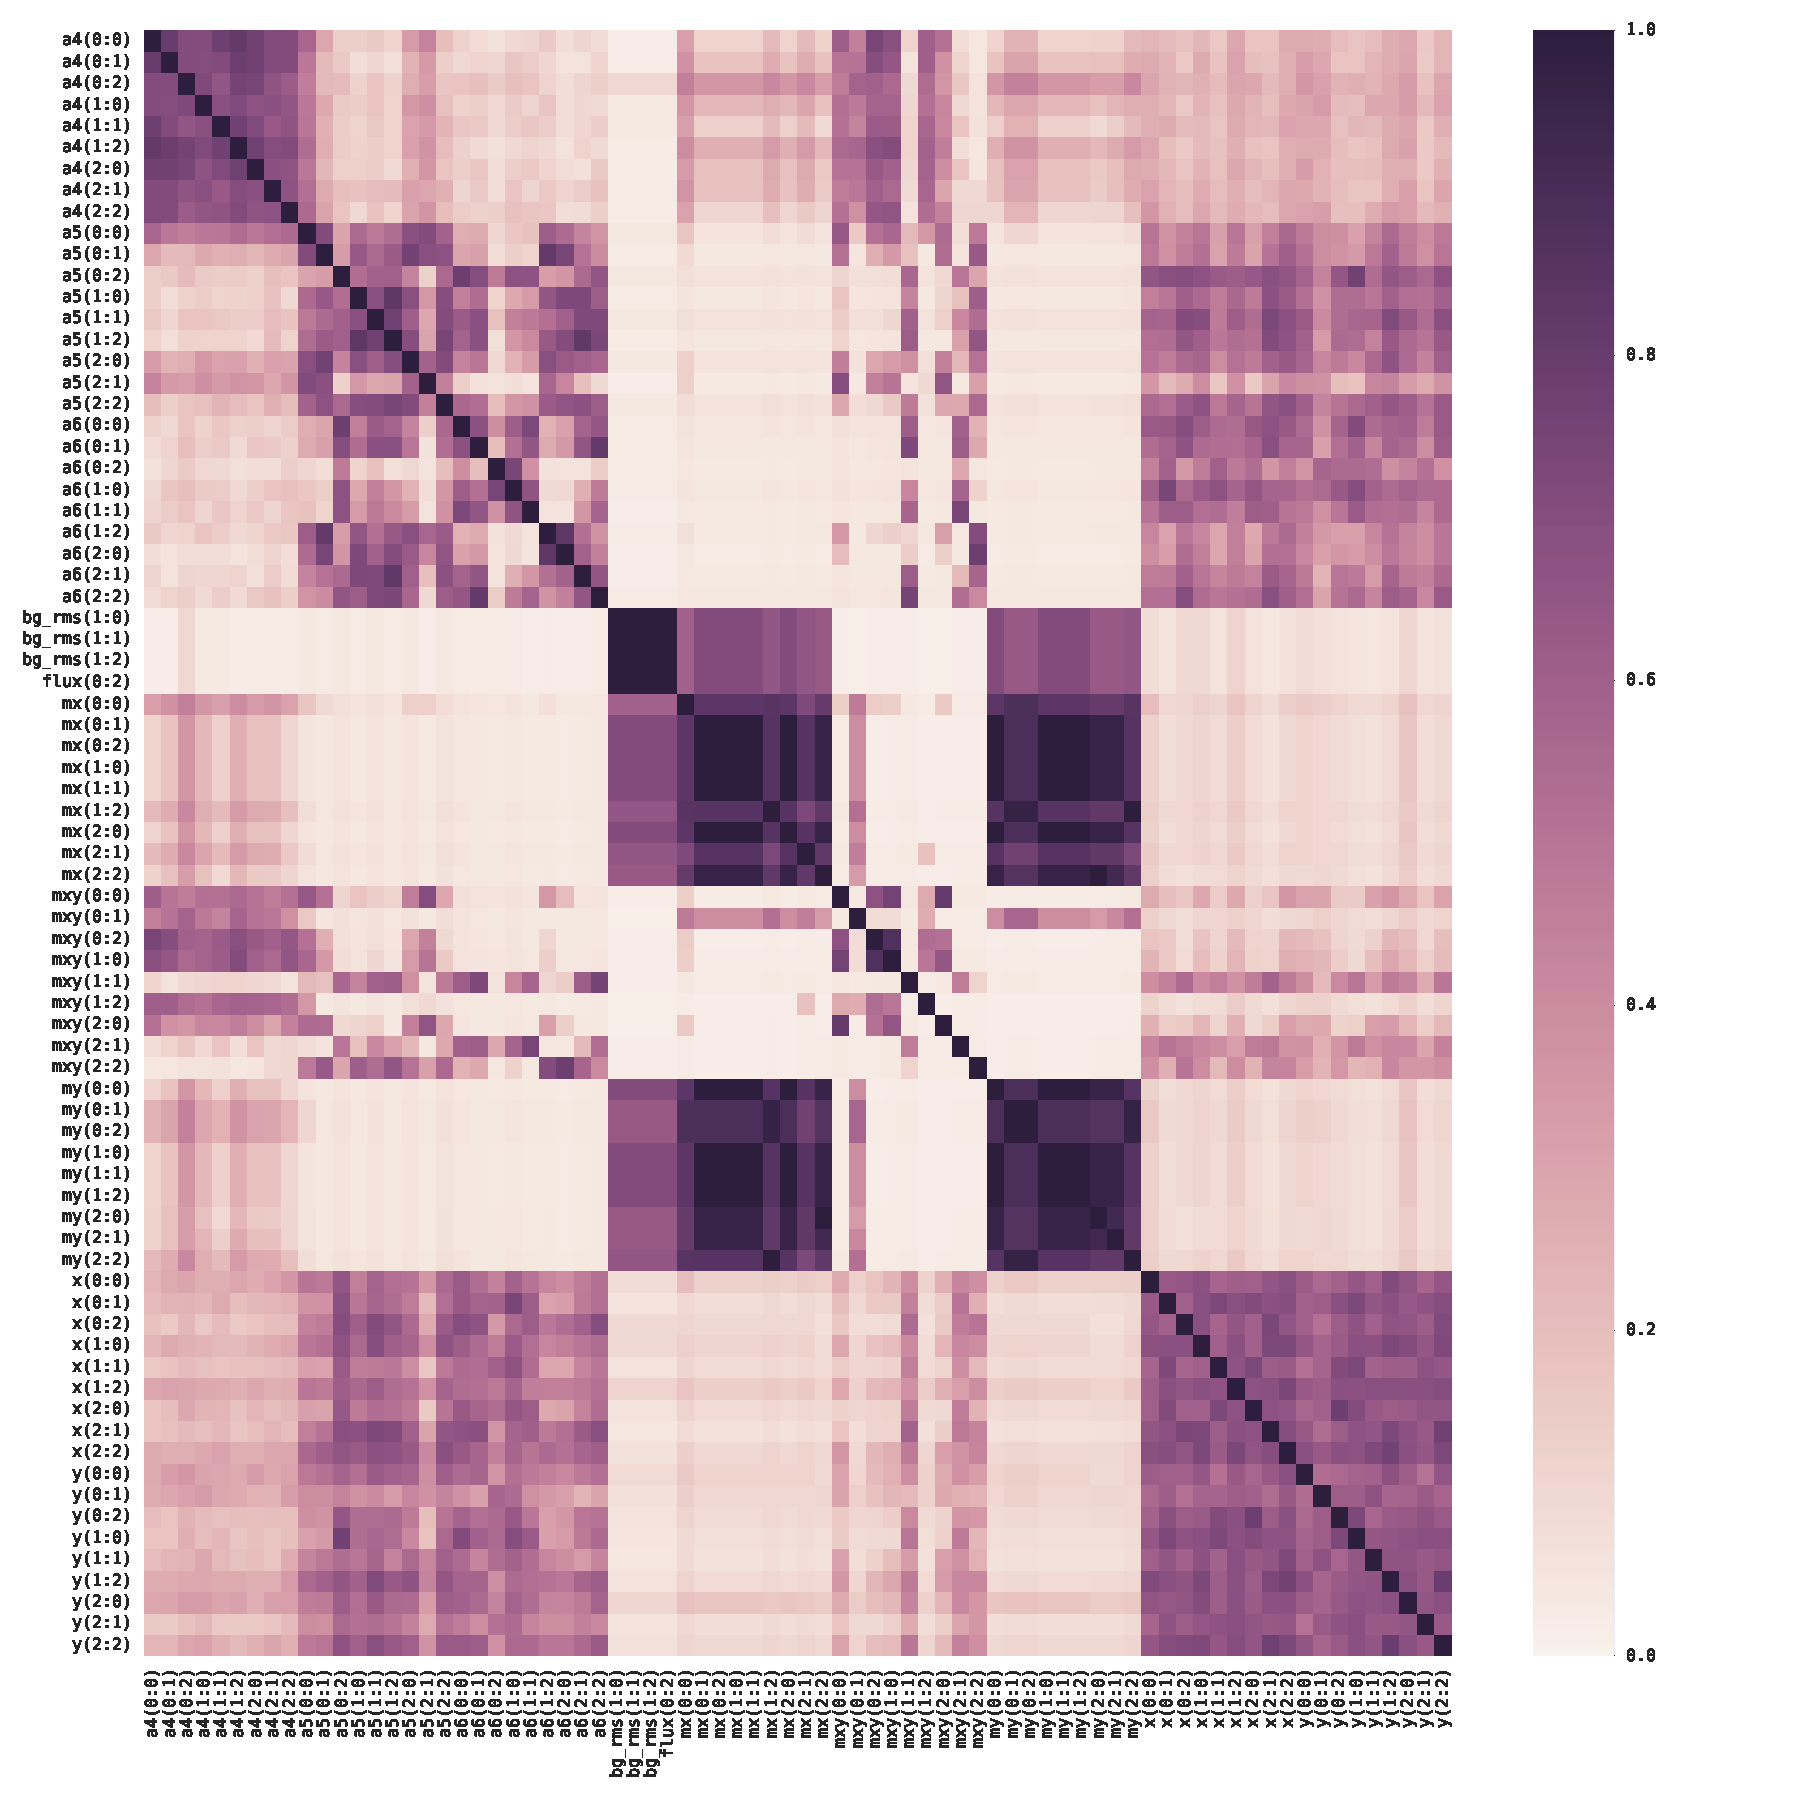
\includegraphics[scale=.56]{heatmaps/psf.pdf}
	\caption[Transinformations-Heatmap der PSF-Parameter]{Transinformations-Heatmap der PSF-Parameter. Jeder Pixel auf der Karte entspricht einem normierten Transinformations-Index. Die Achsen zeigen den Bezeichner des Parameters so wie seine Position innerhalb eines $3\times 3$-Gitters auf dem Sensor.  Da beide Achsen die selben Parameter enthalten nimmt jeder Wert auf der Diagonalen den Wert $\num{1}$ an.}
    \label{heatmap_psf_inline}
\end{figure}

\begin{figure}[H]
	\centering
	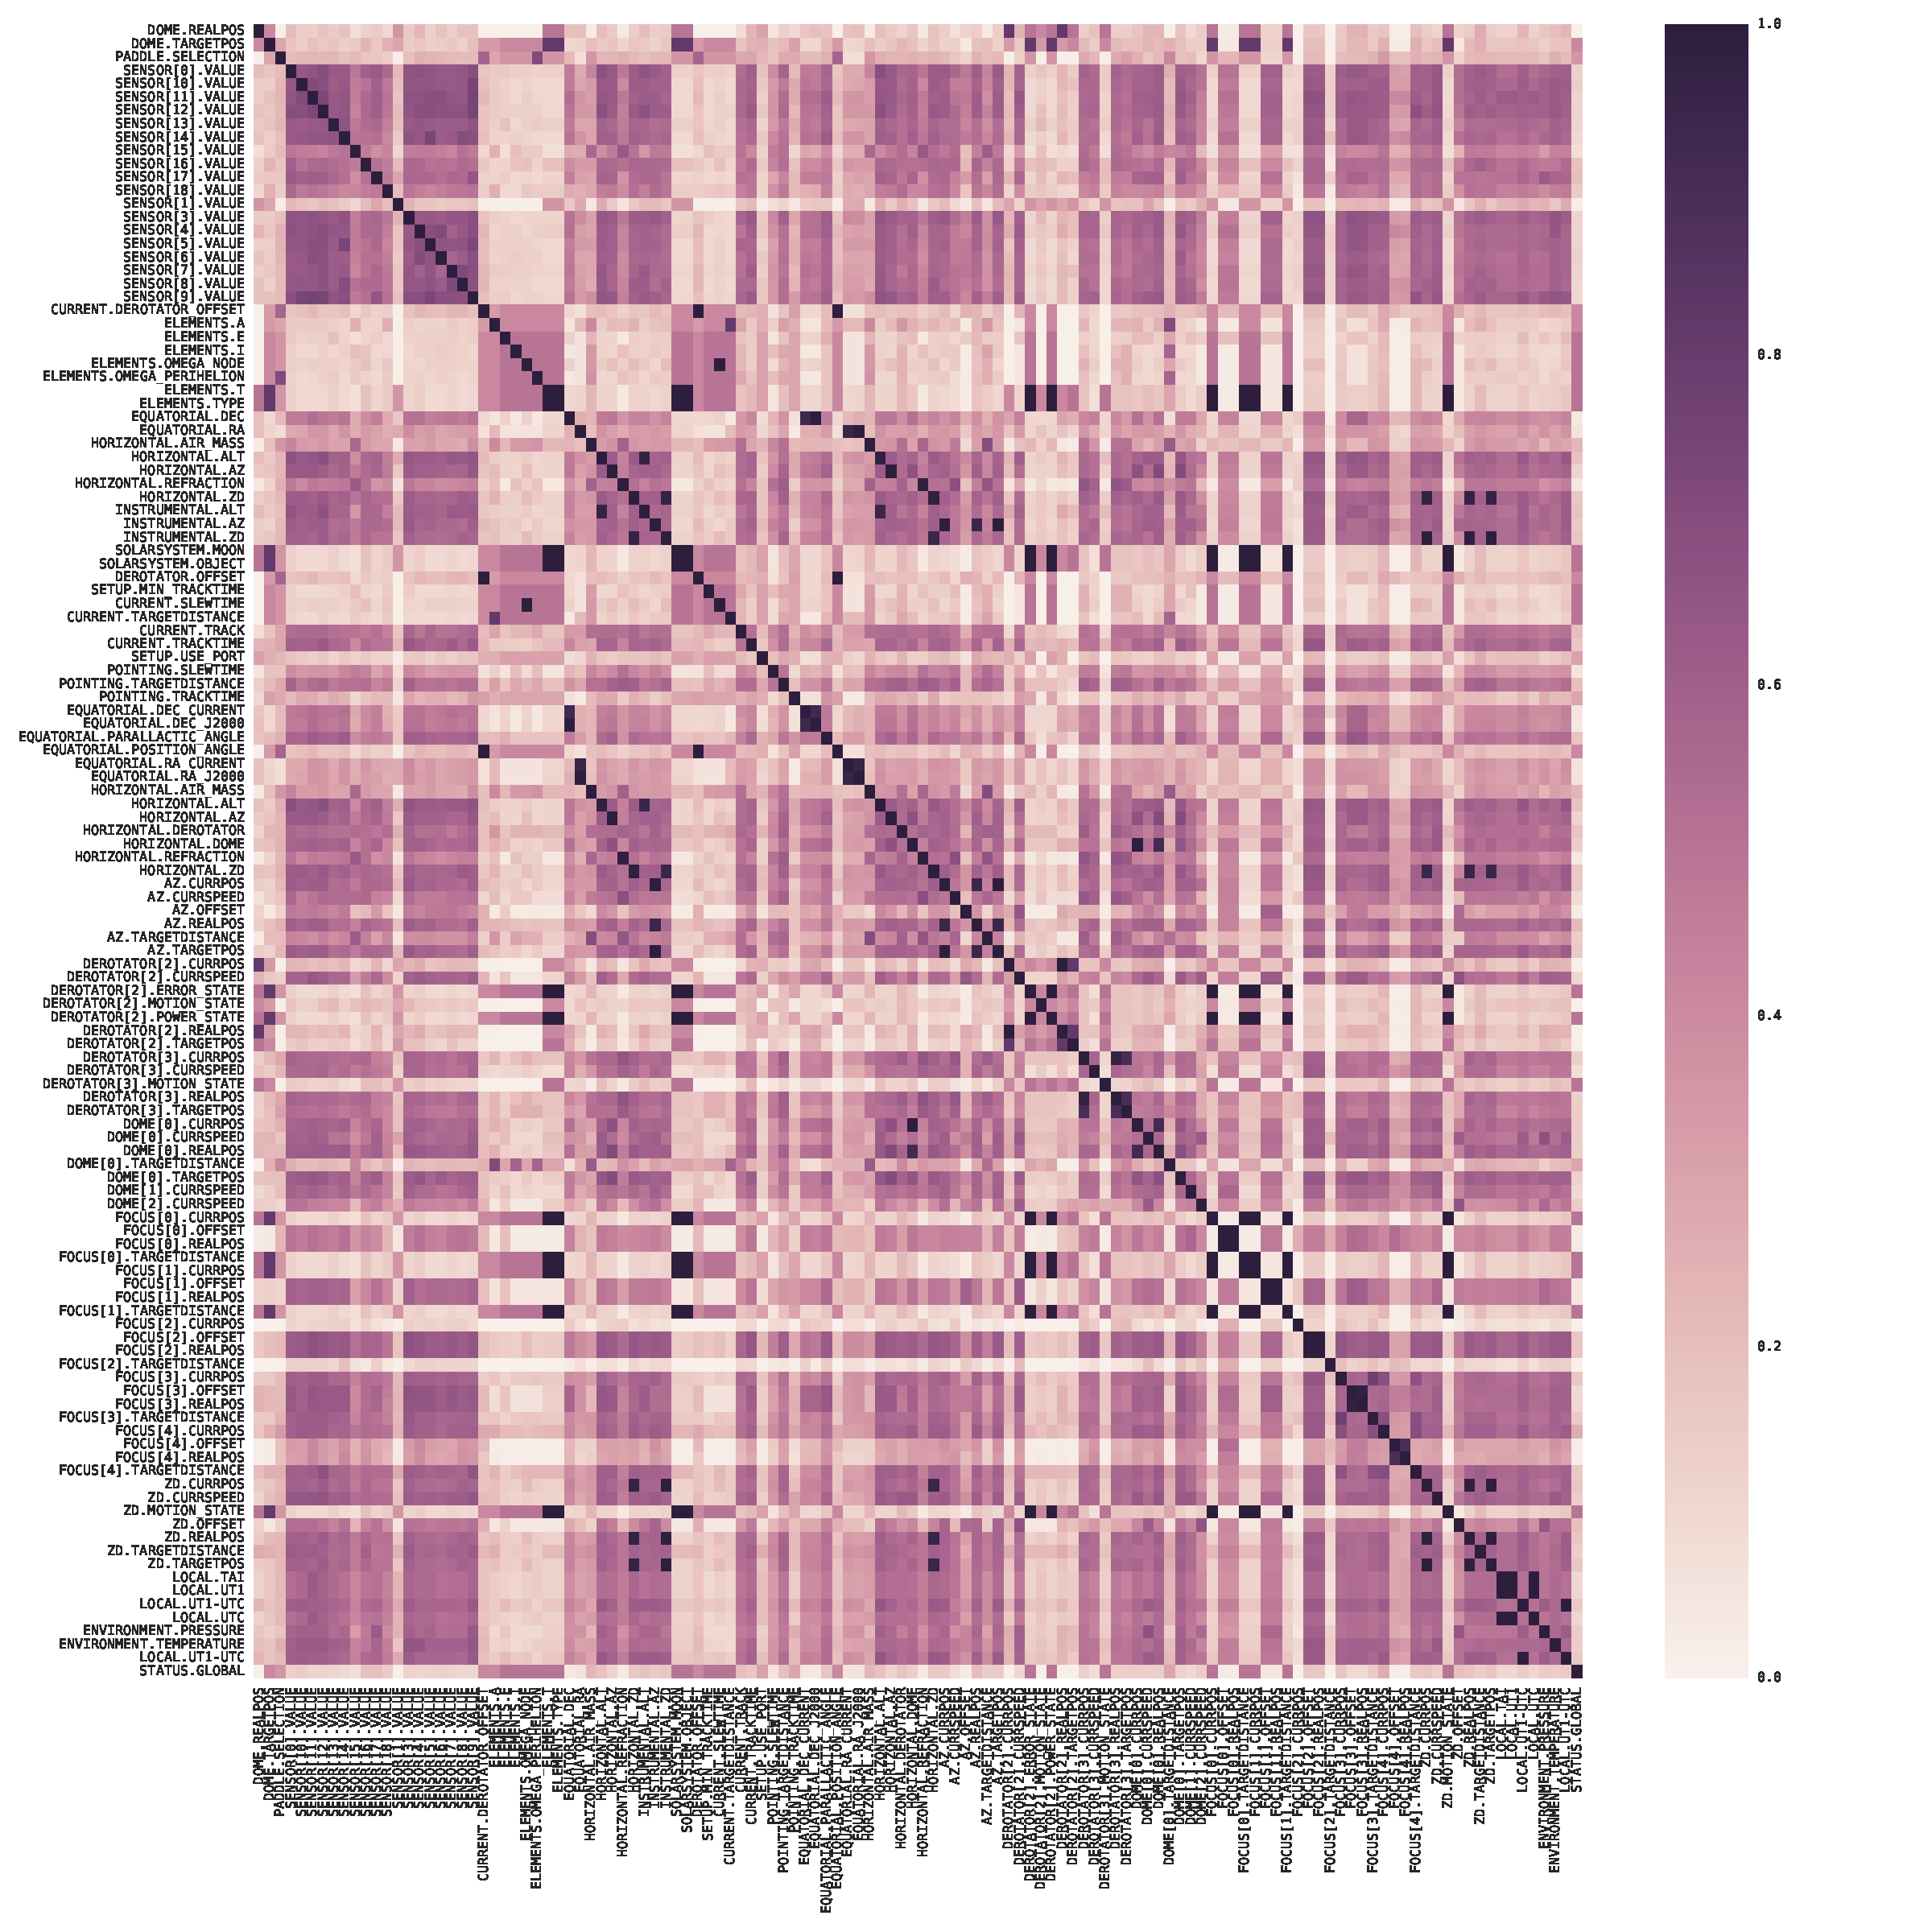
\includegraphics[scale=.42]{heatmaps/tsi.pdf}
	\caption[Transinformations-Heatmap der TSI-Parameter]{Transinformations-Heatmap der TSI-Parameter. Jeder Pixel auf der Karte entspricht einem normierten Transinformations-Index. Da beide Achsen die selben Parameter enthalten nimmt jeder Wert auf der Diagonalen den Wert $\num{1}$ an.}
    \label{heatmap_tsi_inline}
\end{figure}

\begin{figure}[H]
	\centering
	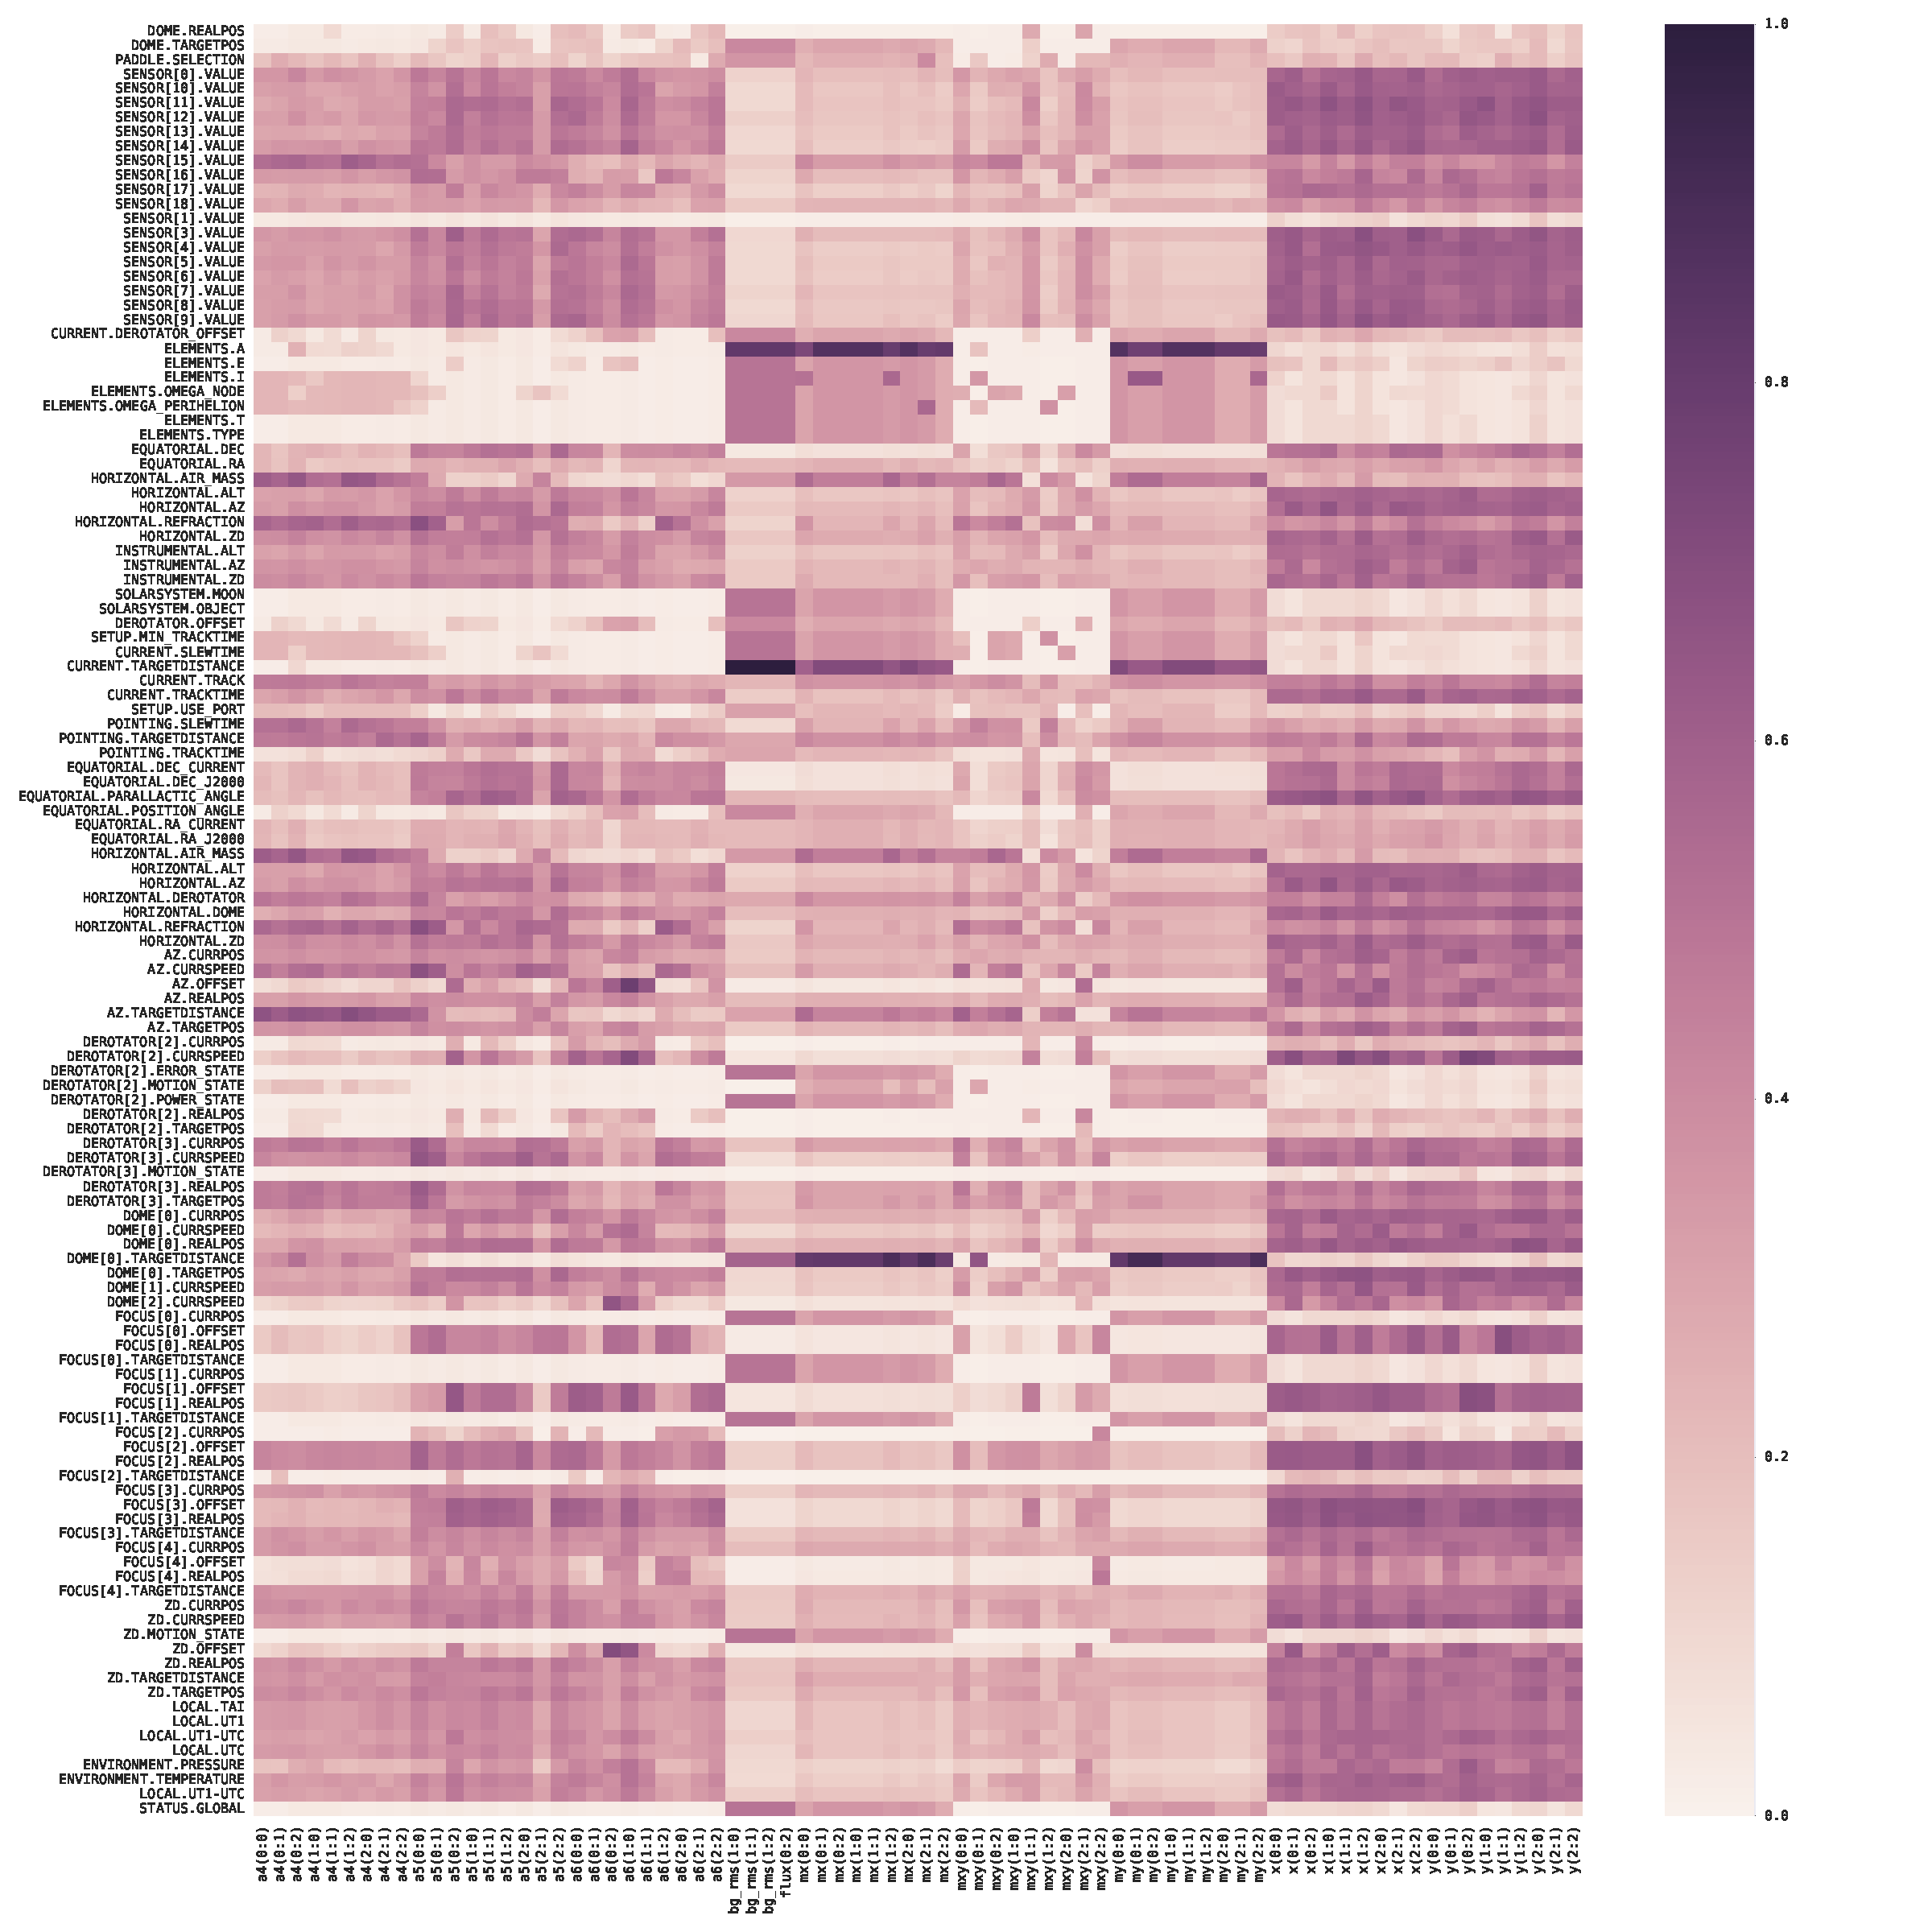
\includegraphics[scale=.42]{heatmaps/psf_tsi.pdf}
	\caption[Heatmap der Transinformation Korrelationsmatrix zwischen PSF- und TSI-Parametern]{Heatmap der Transinformation Korrelationsmatrix zwischen PSF- und TSI-Parametern. Jeder Pixel auf der Karte entspricht einem normierten Transinformations-Index.}
    \label{heatmap_psf_tsi_inline}
\end{figure}

Bei allen drei Matrizen fällt auf, dass sich Blöcke mit ähnlichen Transinformationswerten bilden. In erster Näherung kann dies durch die natürliche Gruppierung der Parameter auf den Achsen erklärt werden. Im Falle einer PSF-Achse wird jeder Parameter mehrfach aufgeführt (einmal für jeden Durchschnittswert im Gitter). Da sich die Position auf dem Detektor nur durch ein geringfügiges Rauschen äußert (vgl. \ref{psf_dists}) verhalten sich gleiche PSF-Parameter unterschiedlicher Gitterposition stochastisch sehr ähnlich. Bei einer TSI-Achse tauchen Parameter mit ähnlicher Verteilung auf, die aufgrund der alphabetischen Sortierung gruppiert werden. Oft sind dies Parameter und ihr Offset oder der selbe Parameter mit unterschiedlichem Namen. Beide Gruppierungen stochastisch ähnlicher Verteilungen auf den Achsen äußern sich in der geplotteten Matrix als Blöcke mit ähnlichem Wert.\\
Darüber hinaus gibt es hohe Korrelationswerte die kein bestimmtes Muster aufweisen und individuell betrachtet werden müssen. Besonders interessant sind Korrelationen mit der Position des Sekundärspiegels, da diese auf weitere Abhängigkeiten hinweisen könnten, welche in der Fokusfunktion zu berücksichtigen sind. Das die Transinformation ein guter Anhaltspunkt ist, bestätigen auch die bekannten Relationen. So wird die Sekundärspiegelposition mit Werten von $\sim\num{0.7}$ in der Korrelationsmatrix deutlich mit Temperatursensoren und Elevationsparametern korreliert.

\begin{figure}[H]
	\centering
	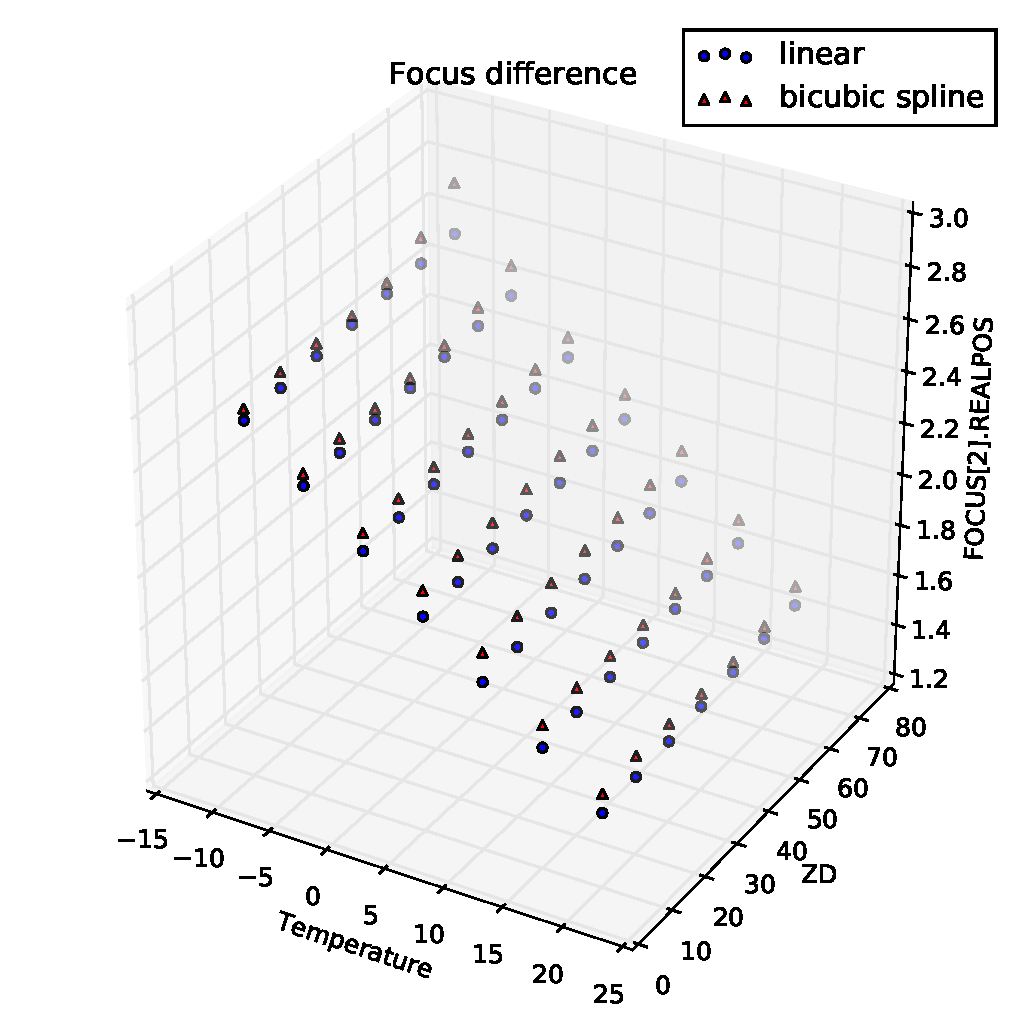
\includegraphics[scale=.6]{diff.pdf}
	\caption[Sekundärspiegelposition der linearen und bikubischen Näherung]{Sekundärspiegelposition der linearen und bikubischen Näherung. Es werden die absoluten Sekundärspiegelpositionen der beiden Fokusfunktionen für ausgewählte Punkte in Abhängigkeit von Temperatur und Elevation dargestellt.}
    \label{focus_surf}
\end{figure}

\subsection{Fokusfunktion}
Die Fokusfunktion wie sie momentan im Fraunhofer Teleskop Anwendung findet, justiert den Sekundärspiegel nur entlang der optischen Achse. Es wird folglich nur der Defokus berücksichtigt -- eine etwaige Berücksichtigung oder Korrektur des Astigmatismus erfolgt nicht. Der entsprechende Aberrations-Koeffizient ist $A_4$.\\
Eine Betrachtung von $A_4$ zeigt, dass die Median-Werte für hohe Temperaturen bei mittlerer Elevation stark zunehmen (Abb. \ref{psf_surf_a4_med_inline}). Im Allgemeinen streut $A_4$ eher stark, insbesondere bei hohen Temperaturen (Abb. \ref{psf_surf_a4_std_inline}). Bei diesen Plots wurden nur die als Beste ausgewählten Aufnahmen der jeweiligen Fokusserie verwendet.\\
Um auszuschließen, dass Seeing für die schlechten $A_4$ Werte bei hohen Temperaturen verantwortlich ist, kann die Windgeschwindigkeit und Windrichtung herangezogen werden. Die Verteilung hoher $A_4$ Werte im Polarplot zeigt keine ausgezeichneten Muster auf (Abb. \ref{wind_a4_inline}). Insbesondere sind für hohe Windgeschwindigkeiten aus südlicher Richtung (\enquote{Föhn}) keine schlechten $A_4$ Werte festzustellen. Insgesamt ist es somit naheliegend, dass weniger das Wetter als der durch die Temperatur auf das System ausgeübte Stress für den Defokus der Aufnahmen verantwortlich ist.\\

\begin{figure}[H]
	\centering
	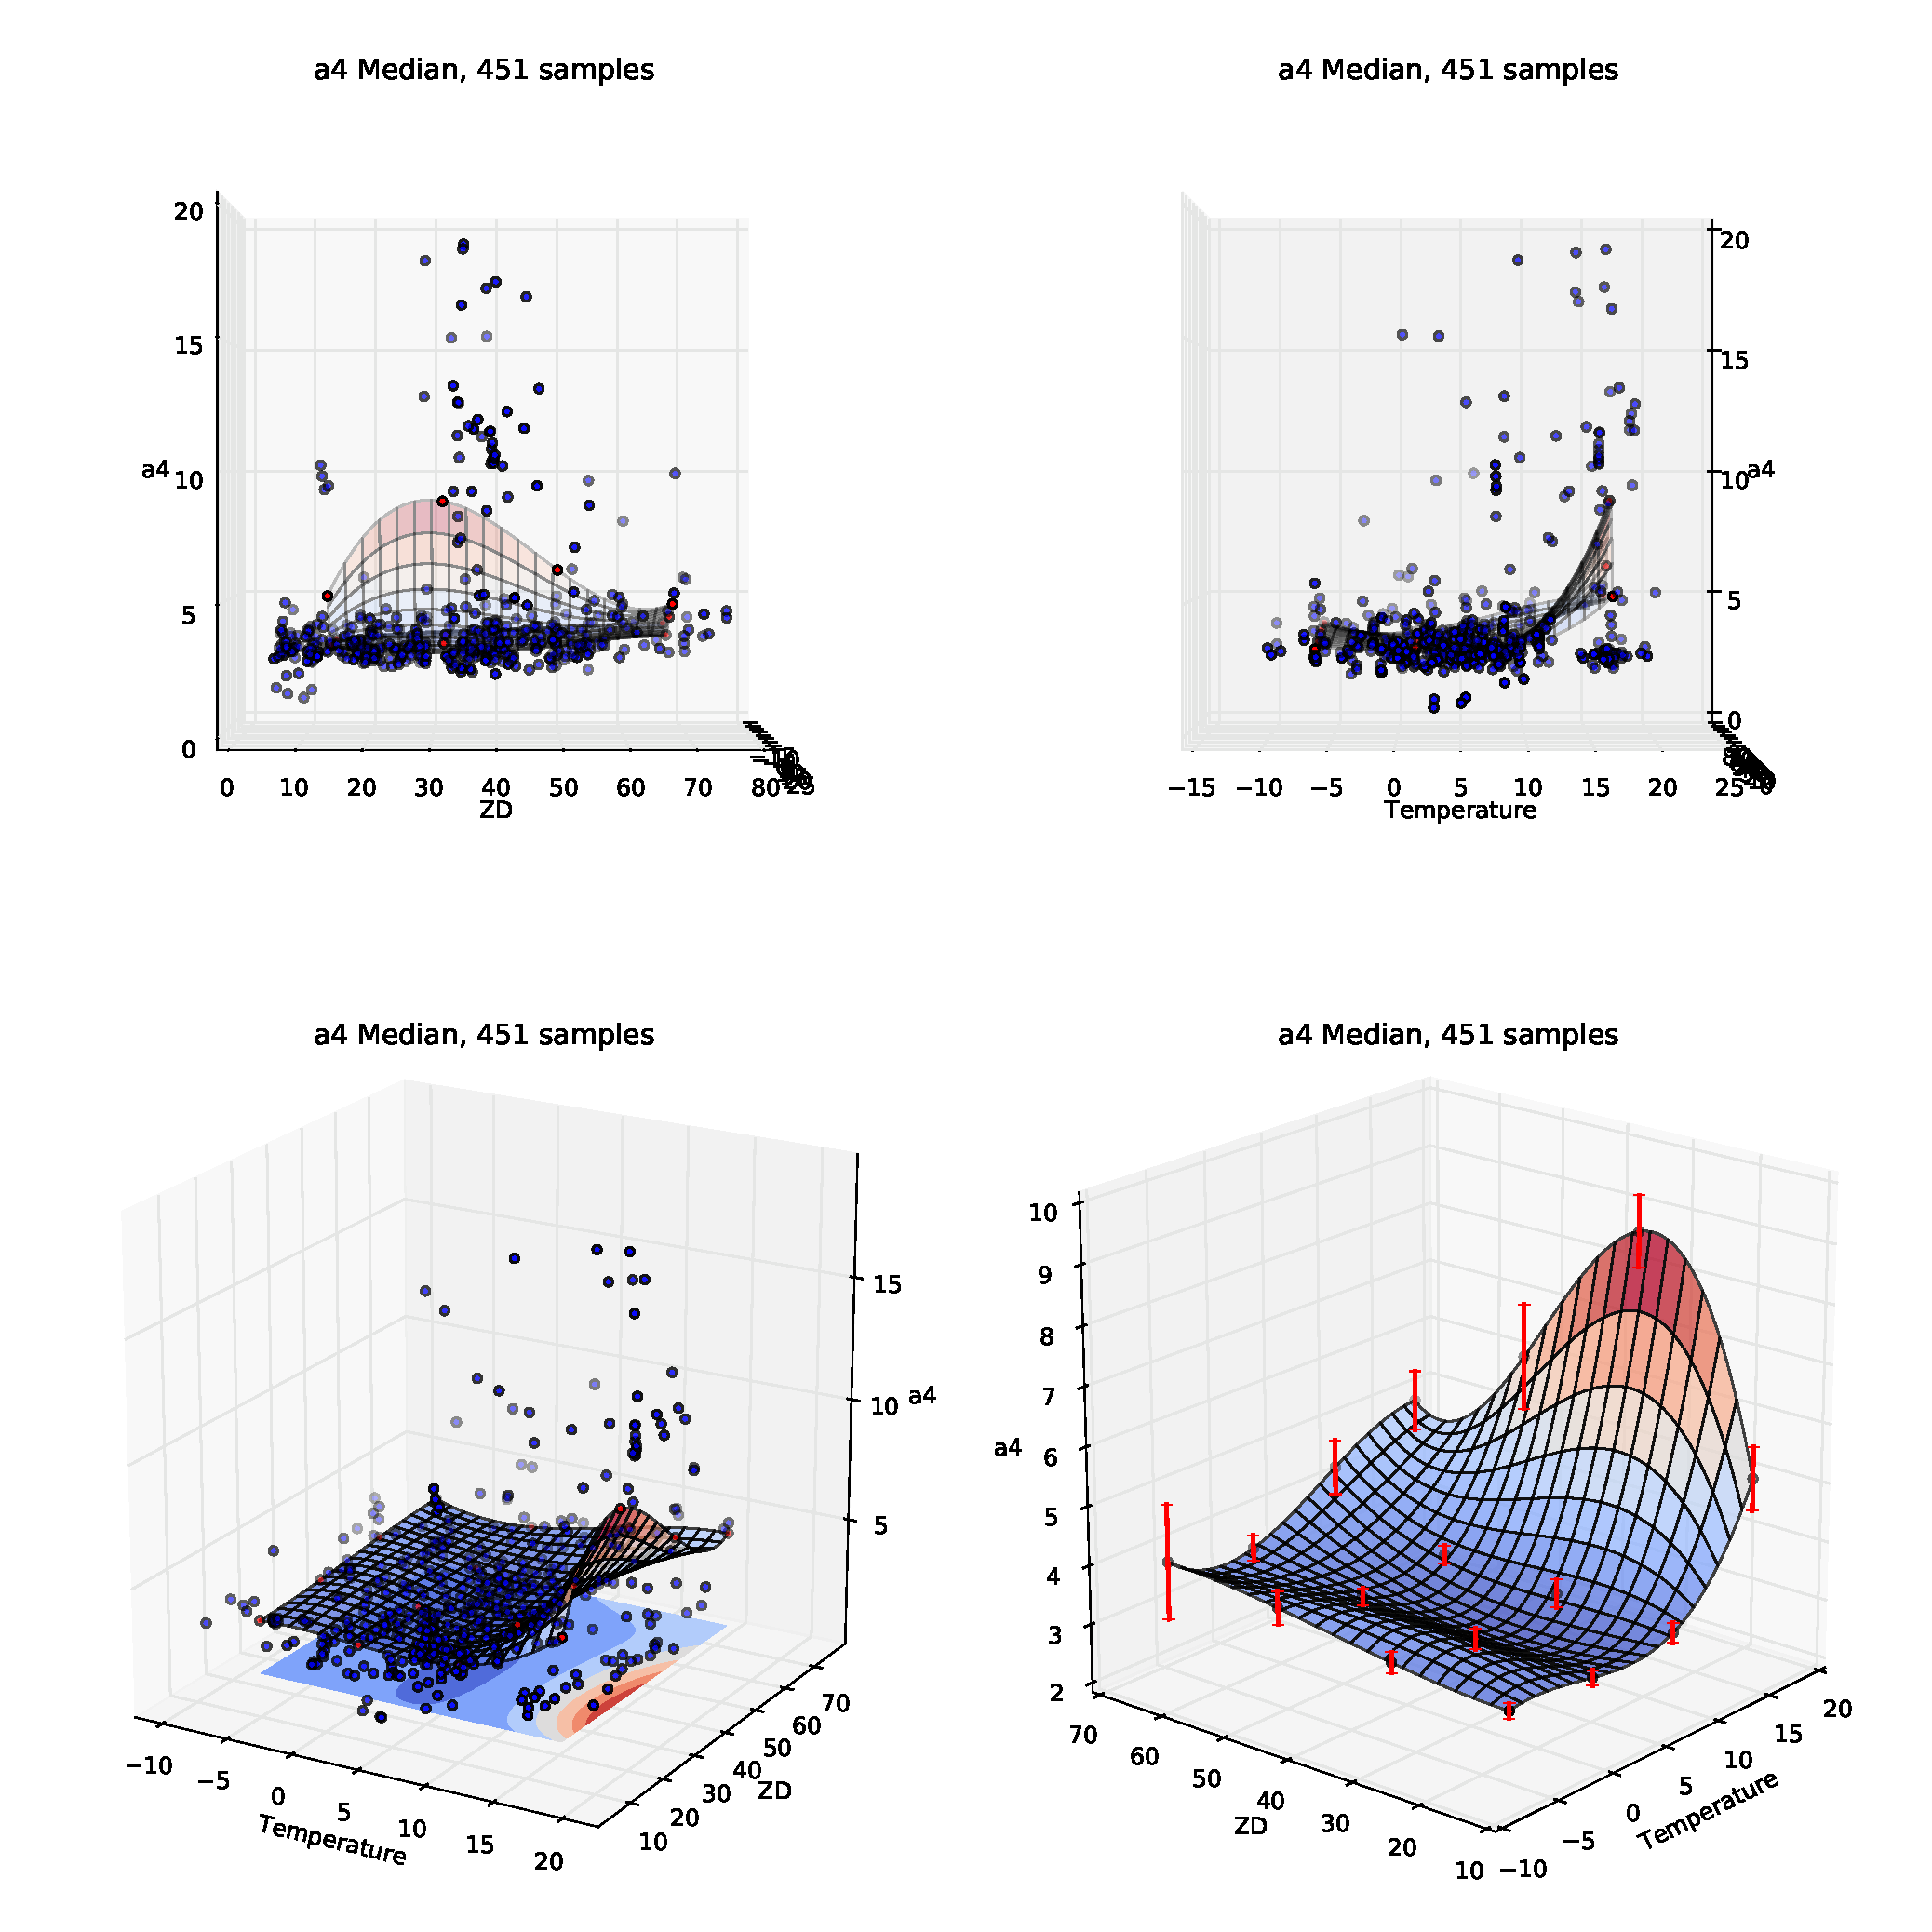
\includegraphics[scale=.48]{psf_surf/a4_med.pdf}
	\caption[Median Temperatur- und Elevationsabhängigkeit von $A_4$]{Median Temperatur- und Elevationsabhängigkeit von $A_4$. Es liegen 451 Fokusaufnahmen zugrunde, die jeweils einem blauen Punkt entsprechen. Die Plots oben links und rechts entsprechen der Projektion auf die Temperatur- und Elevations-Achse respektive. Die roten Kontrollpunkt wurden als Durchschnittswerte berechnet (mean). Die roten Balken an den Kontrollpunkten im Plot unten rechts sind ein Maß für die Streuung des Kontrollpunktes. }
    \label{psf_surf_a4_med_inline}
\end{figure}
\begin{figure}[H]
	\centering
	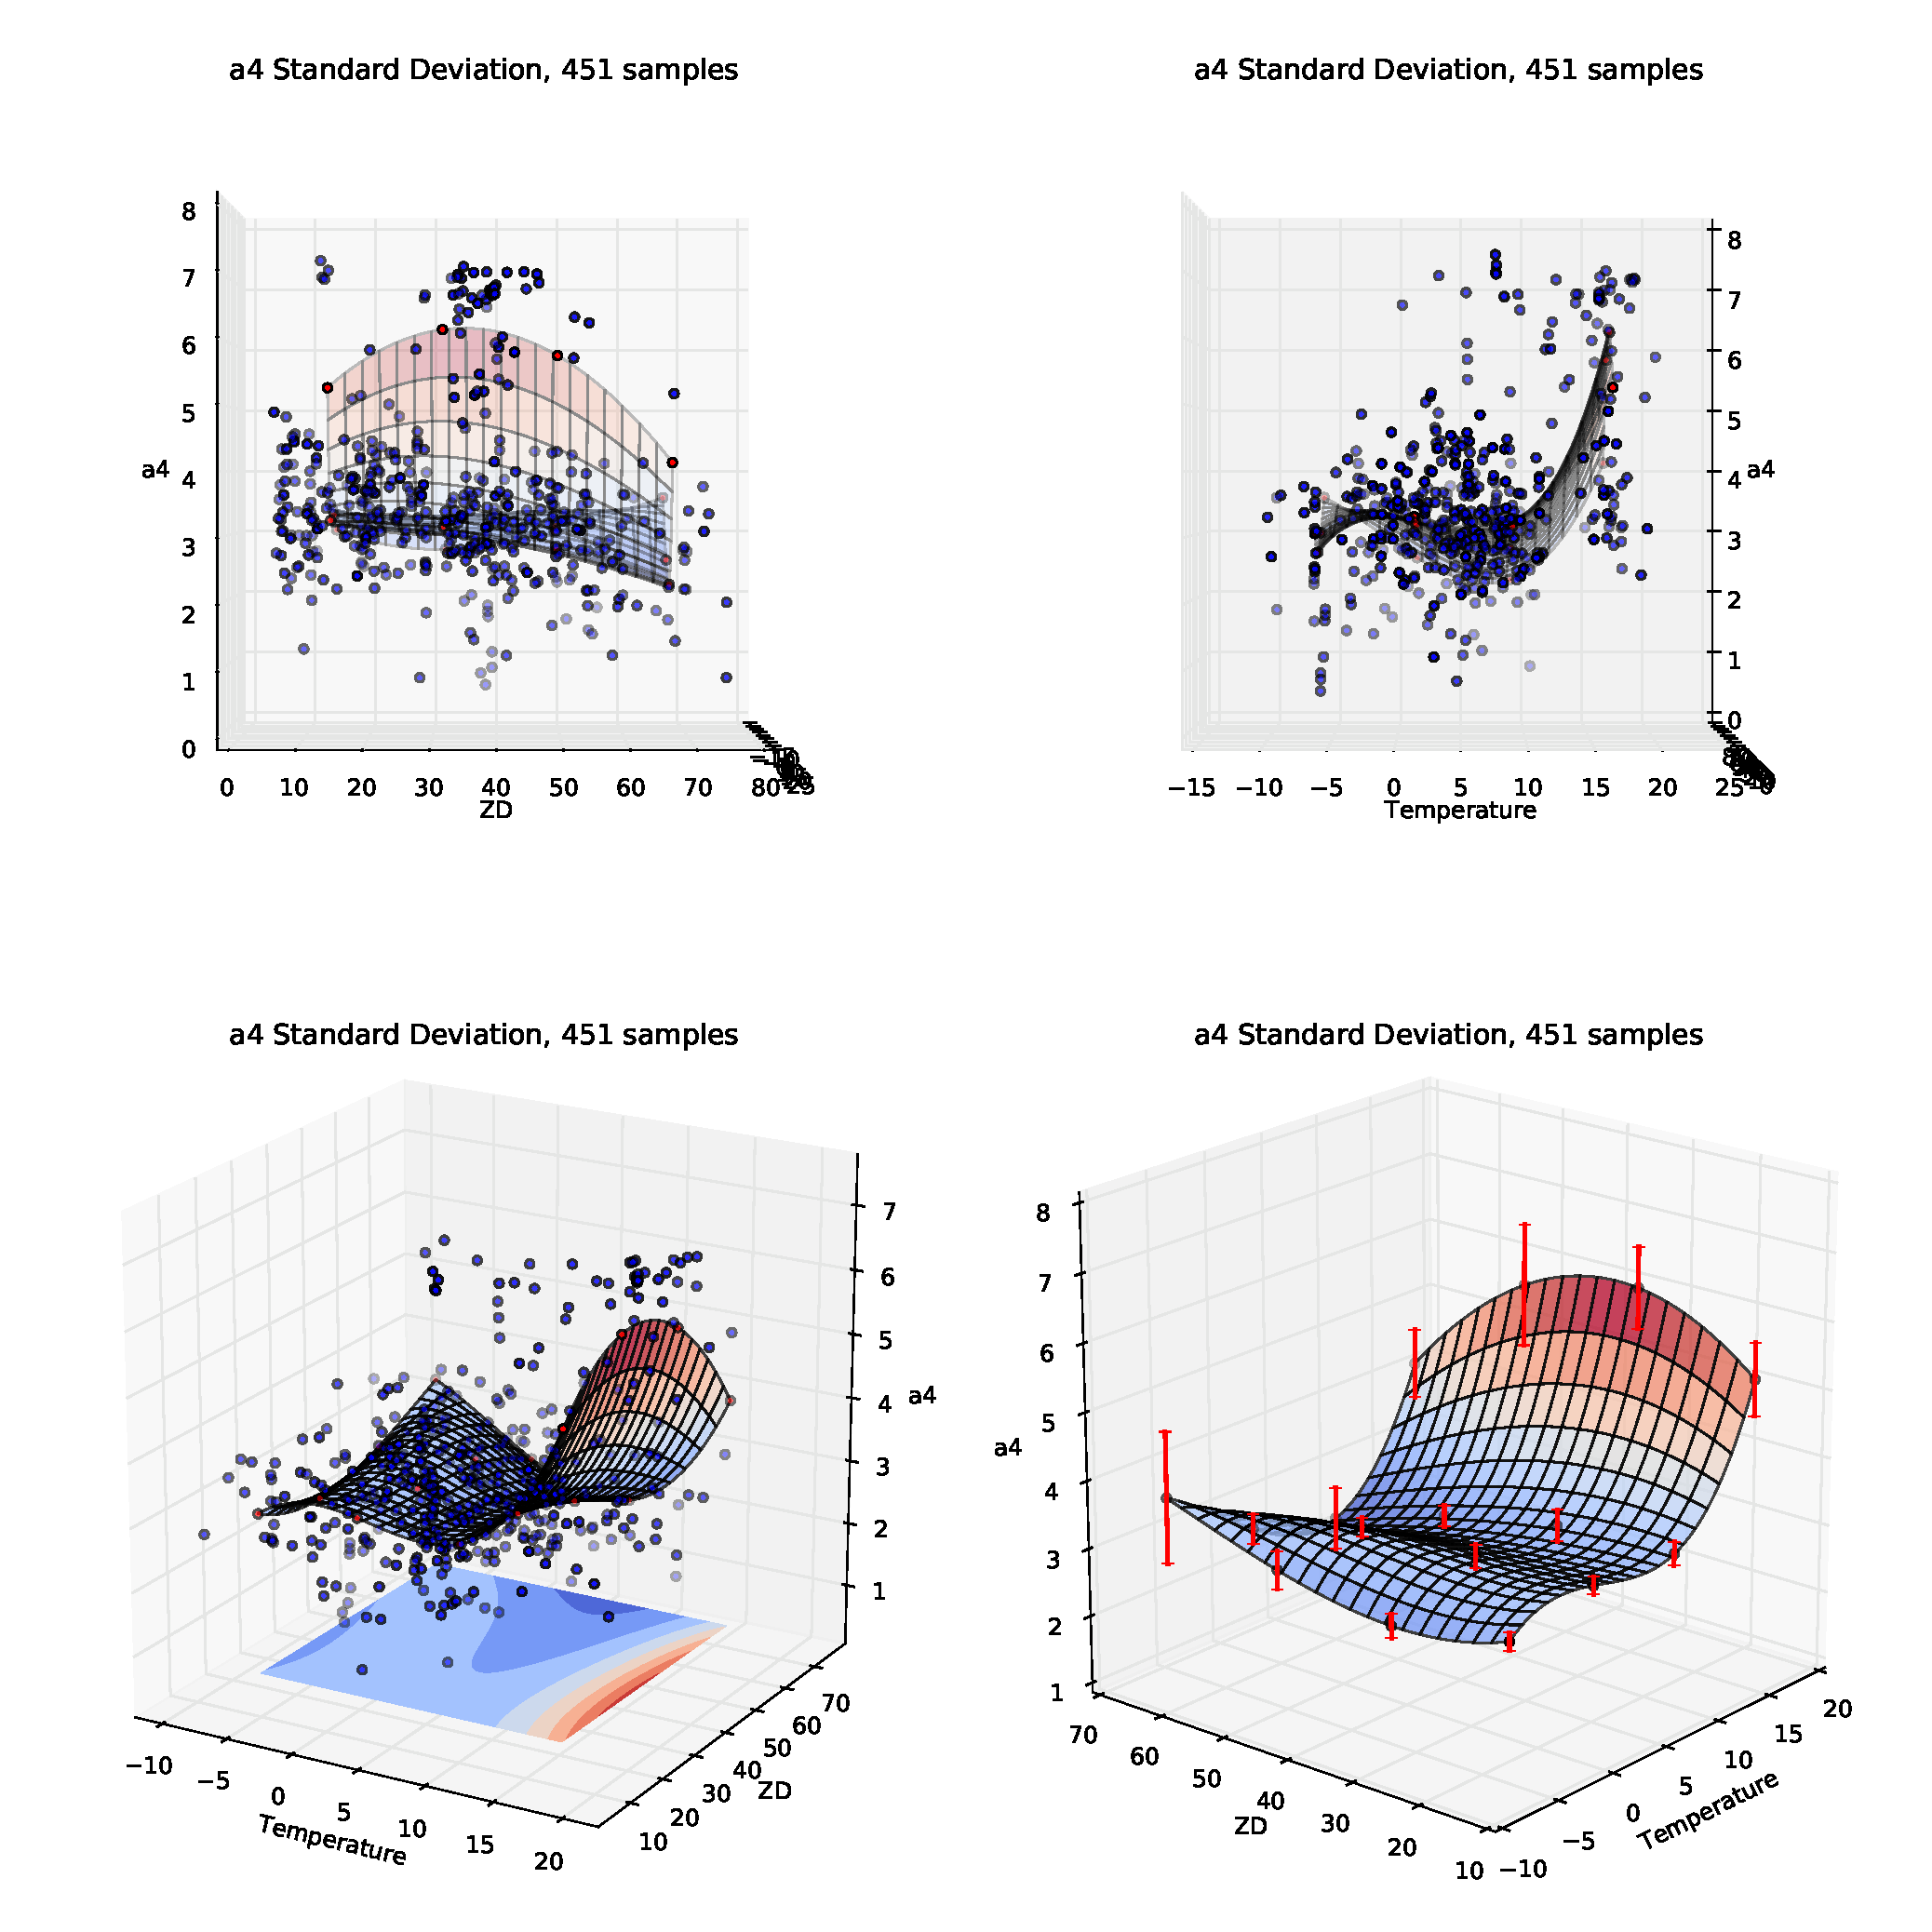
\includegraphics[scale=.48]{psf_surf/a4_std.pdf}
	\caption[Standardabweichung Temperatur- und Elevationsabhängigkeit von $A_4$]{Standardabweichung Temperatur- und Elevationsabhängigkeit von $A_4$. Es liegen 451 Fokusaufnahmen zugrunde, die jeweils einem blauen Punkt entsprechen. Die Plots oben links und rechts entsprechen der Projektion auf die Temperatur- und Elevations-Achse respektive. Die roten Kontrollpunkt wurden als Durchschnittswerte berechnet (mean). Die roten Balken an den Kontrollpunkten im Plot unten rechts sind ein Maß für die Streuung des Kontrollpunktes. }
    \label{psf_surf_a4_std_inline}
\end{figure}
\begin{figure}[H]
	\centering
	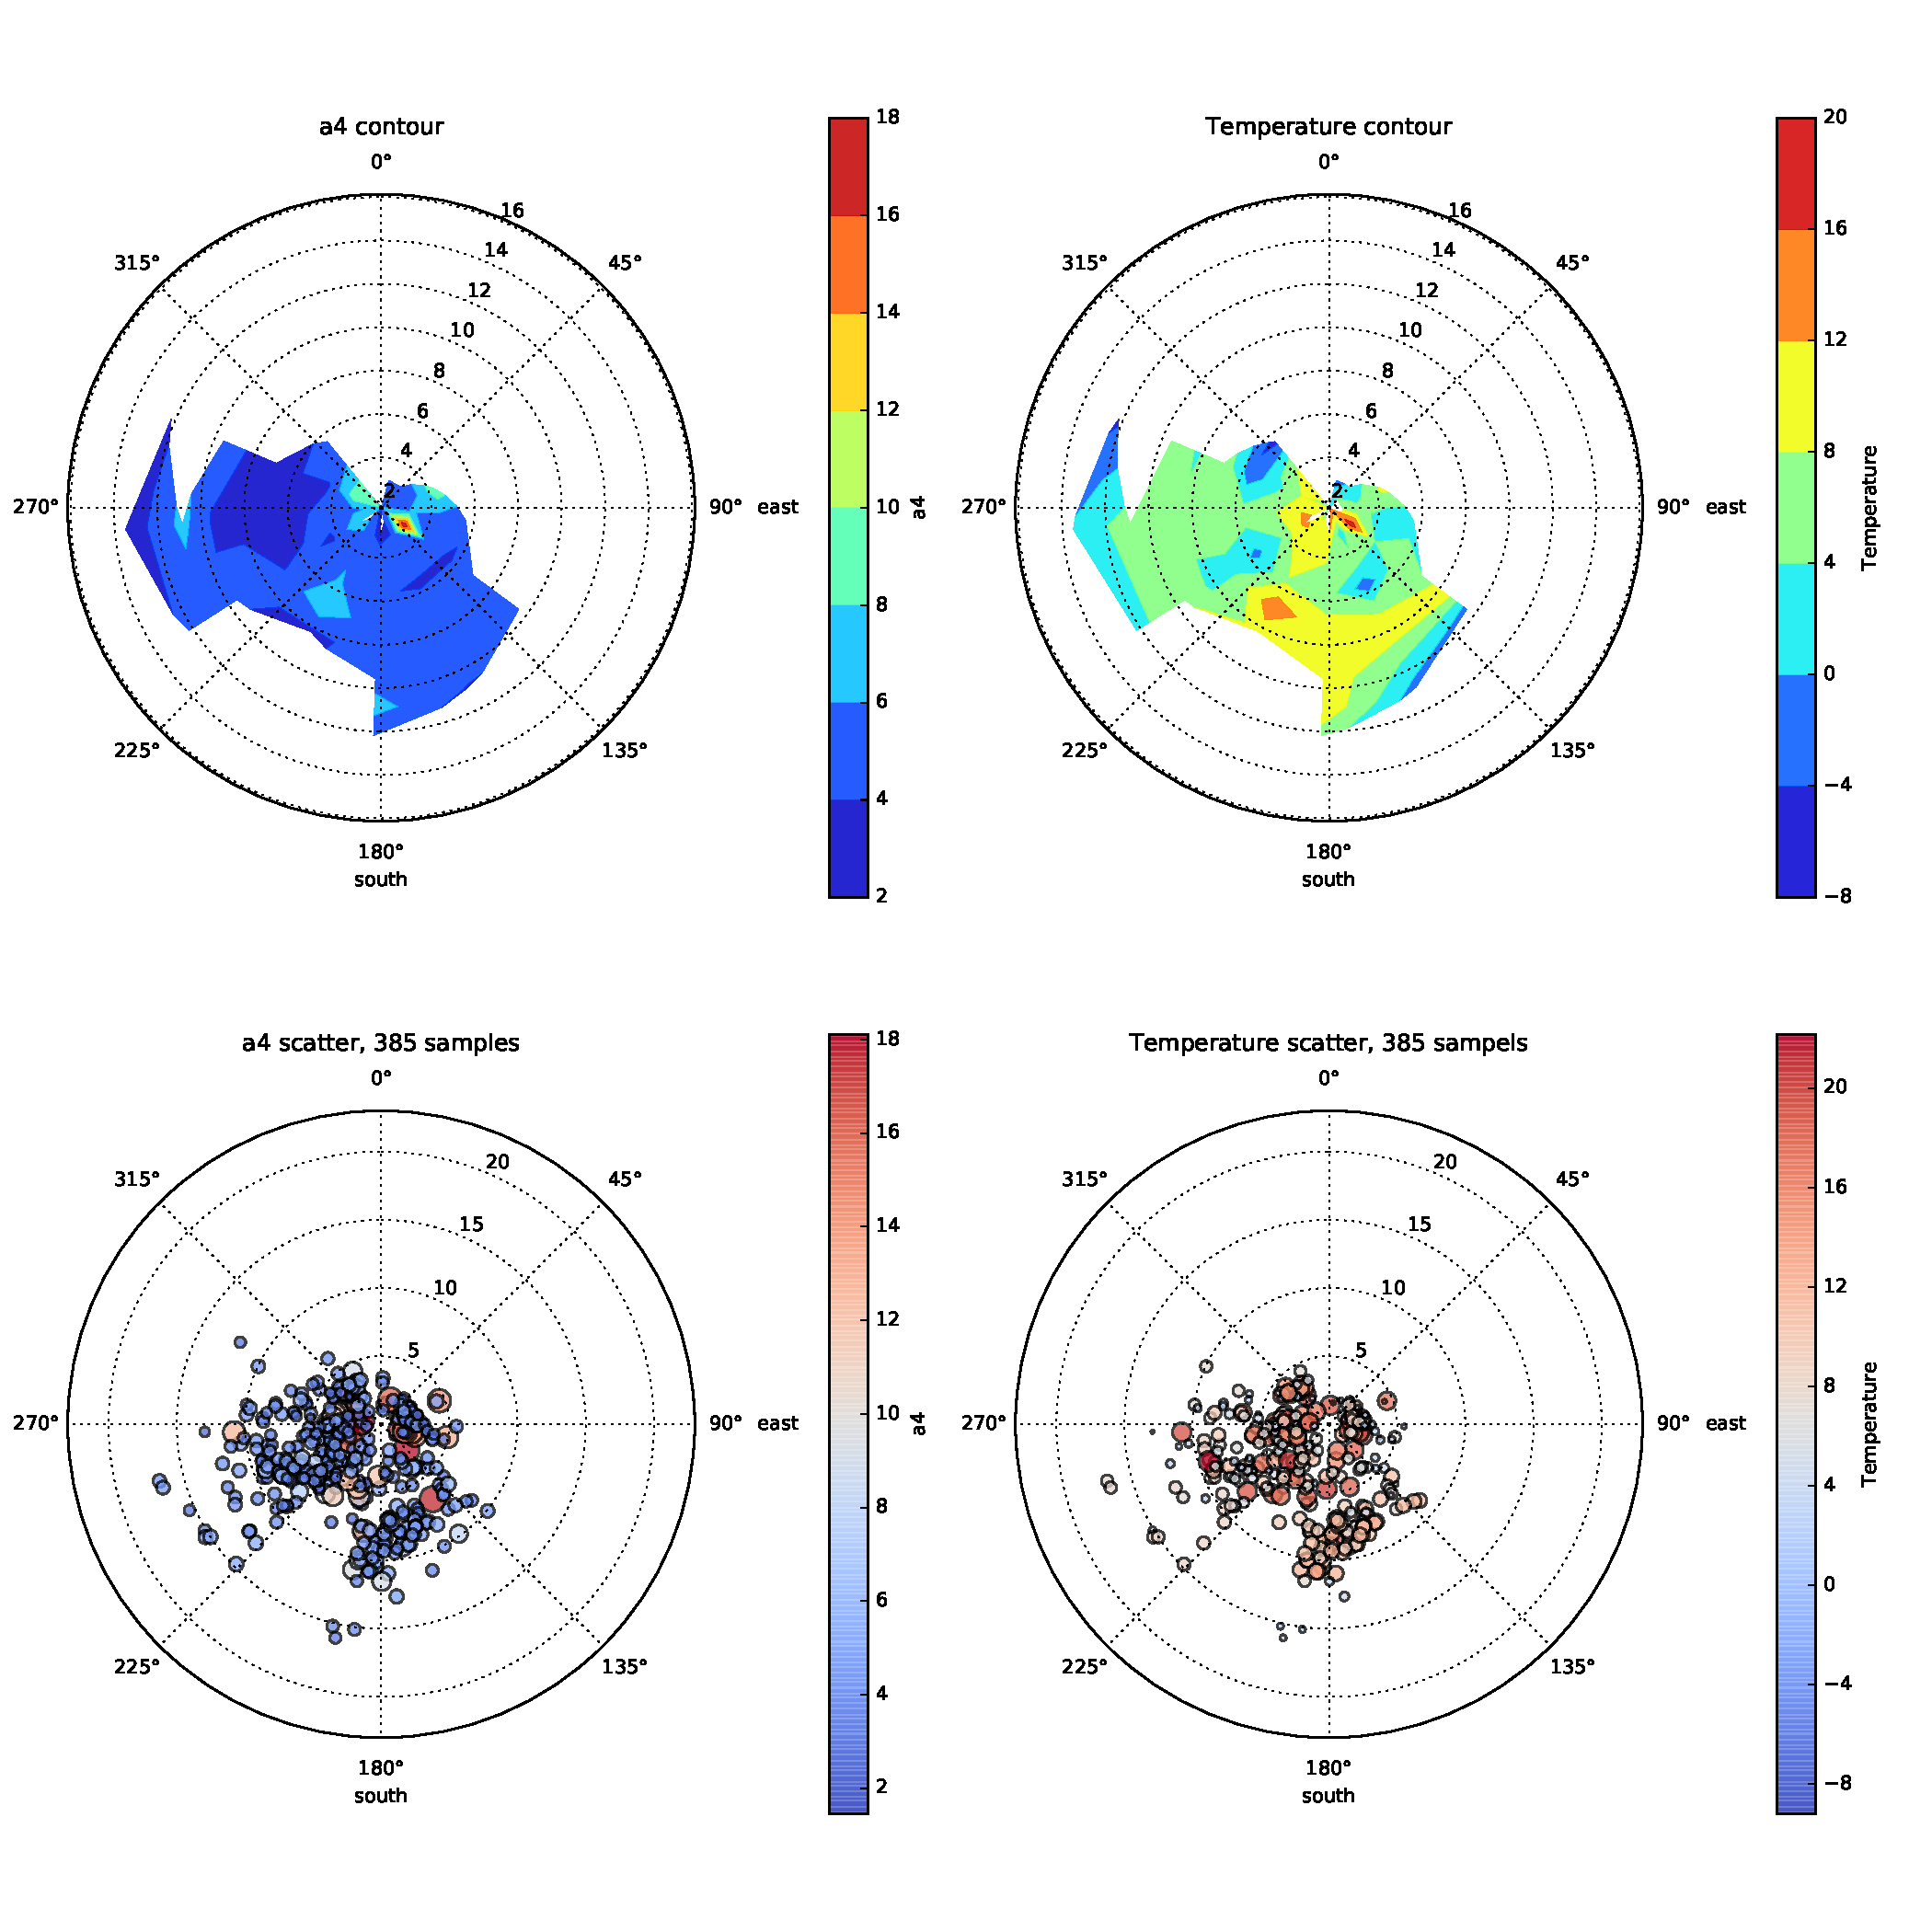
\includegraphics[scale=.46]{wind/wind_a4}
	\caption[Einfluss von Windgeschwindigkeit und Windrichtung auf $A_4$]{Einfluss von Windgeschwindigkeit und Windrichtung auf $A_4$. Die Plots in der linken Spalte zeigen $A_4$ gemäß der Farbskala an. Im unteren Plot ist die Größe der Kreise zusätzlich proportional zu $A_4$. Jeder Kreis repräsentiert eine von 385 Fokusaufnahmen. Analog stellt die rechte Spalte die Temperatur dar. Die Position in Polarkoordinaten wird durch den Wind bestimmt. Der Winkel entspricht der Windrichtung, der Abstand vom Nullpunkt entspricht der Windstärke in \si{\metre\per\second}.}
    \label{wind_a4_inline}
\end{figure}
\pagebreak

Ein Blick auf den Streuplot und den daraus hergeleiteten Flächeninterpolanten macht deutlich, dass die Sekundärspiegelposition und somit der Fokus in erster Linie temperatur- aber auch elevationsabhängig ist (Abb. \ref{foc_med_inline}). Jedoch sind die Isolinien nicht streng linear. Der Fokus in Abhängigkeit der Elevation ist bis zu einem Wert von $\sim\num{.7}$ nahezu konstant und steigt dann näherungsweise linear an. Dieses Verhalten tritt allerdings nur an den Temperaturgrenzbereichen aus. Bei mittleren Temperaturen, verhält sich der Fokus in Abhängigkeit der Elevation nahezu konstant. In Abhängigkeit von der Temperatur verhält sich der Fokus stark linear, zeigt jedoch auch hier leichte Abweichungen: im mittleren Temperaturbereich besteht ein Plateau etwas geringerer Steigung.\\

\begin{figure}[H]
	\centering
	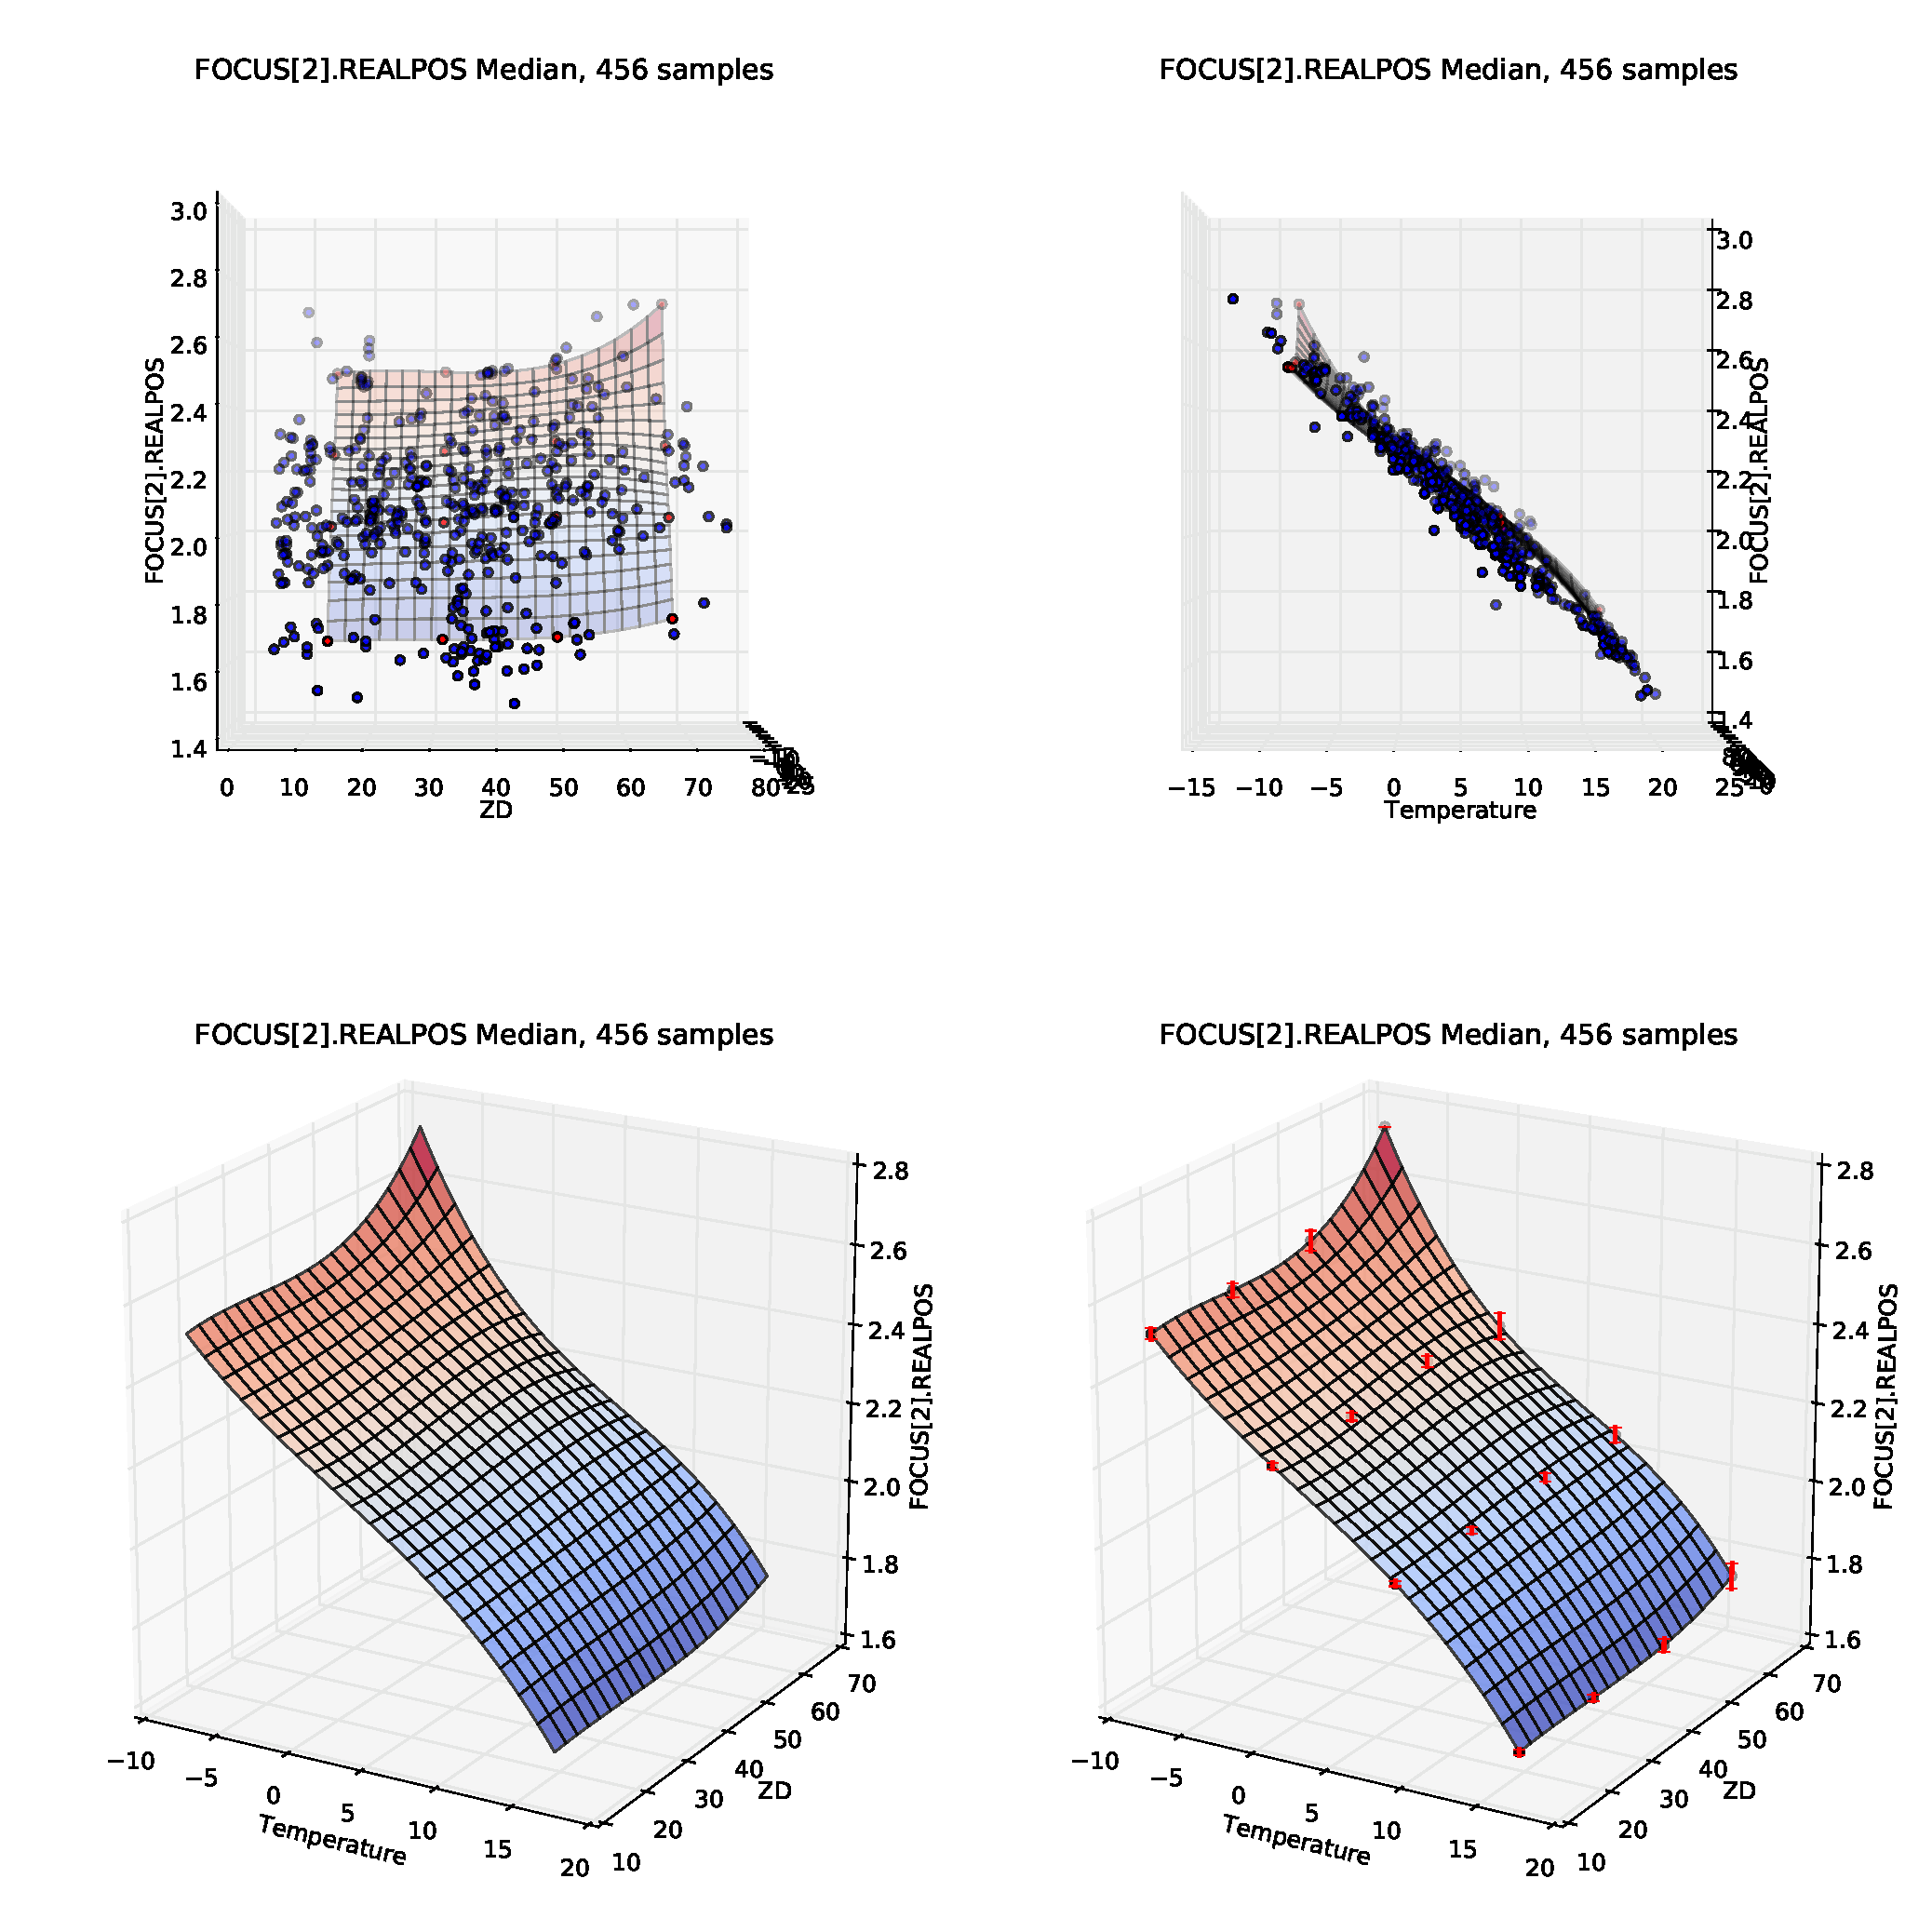
\includegraphics[scale=.44]{tsi_surf/POSITION_INSTRUMENTAL_FOCUS_2__REALPOS_med.pdf}
 	\caption[Temperatur- und Elevationsabhängigkeit der Sekundärspiegelposition]{Temperatur- und Elevationsabhängigkeit der Sekundärspiegelposition entlang der optischen Achse. Die Sekundärspiegelposition von 456 Fokusaufnahmen entsprechen den blauen Punkten. Die roten Kontrollpunkte im Plot unten rechts wurden über den Median aller Punkte in ihrer Umgebung gebildet und enthalten einen roten Fehlerbalken.}
    \label{foc_med_inline}
\end{figure}

Da die Streuung des Fokus in Form von Standardvariation als auch Varianz im Temperatur/Elevations-Raum für die besten Aufnahmen einer Fokusserie mit Werten von $\le\SI{5.0}{\percent}$ nur sehr gering ausfällt (Abb. \ref{psf_surf_a4_std_inline} und \ref{psf_surf_a4_var_inline}), ist der auf den Median-Kontrollpunkten basierende Interpolant der temperatur- und elevationsabhängigen Sekundärspiegelposition ein guter Kandidat für eine präzisere Fokusfunktion. Die B-Spline Fläche wurde als alleinstehendes Python-Skript ausgekoppelt, um in das Teleskop-System eingebunden zu werden (siehe \ref{focus.py}).

\begin{figure}[H]
	\centering
	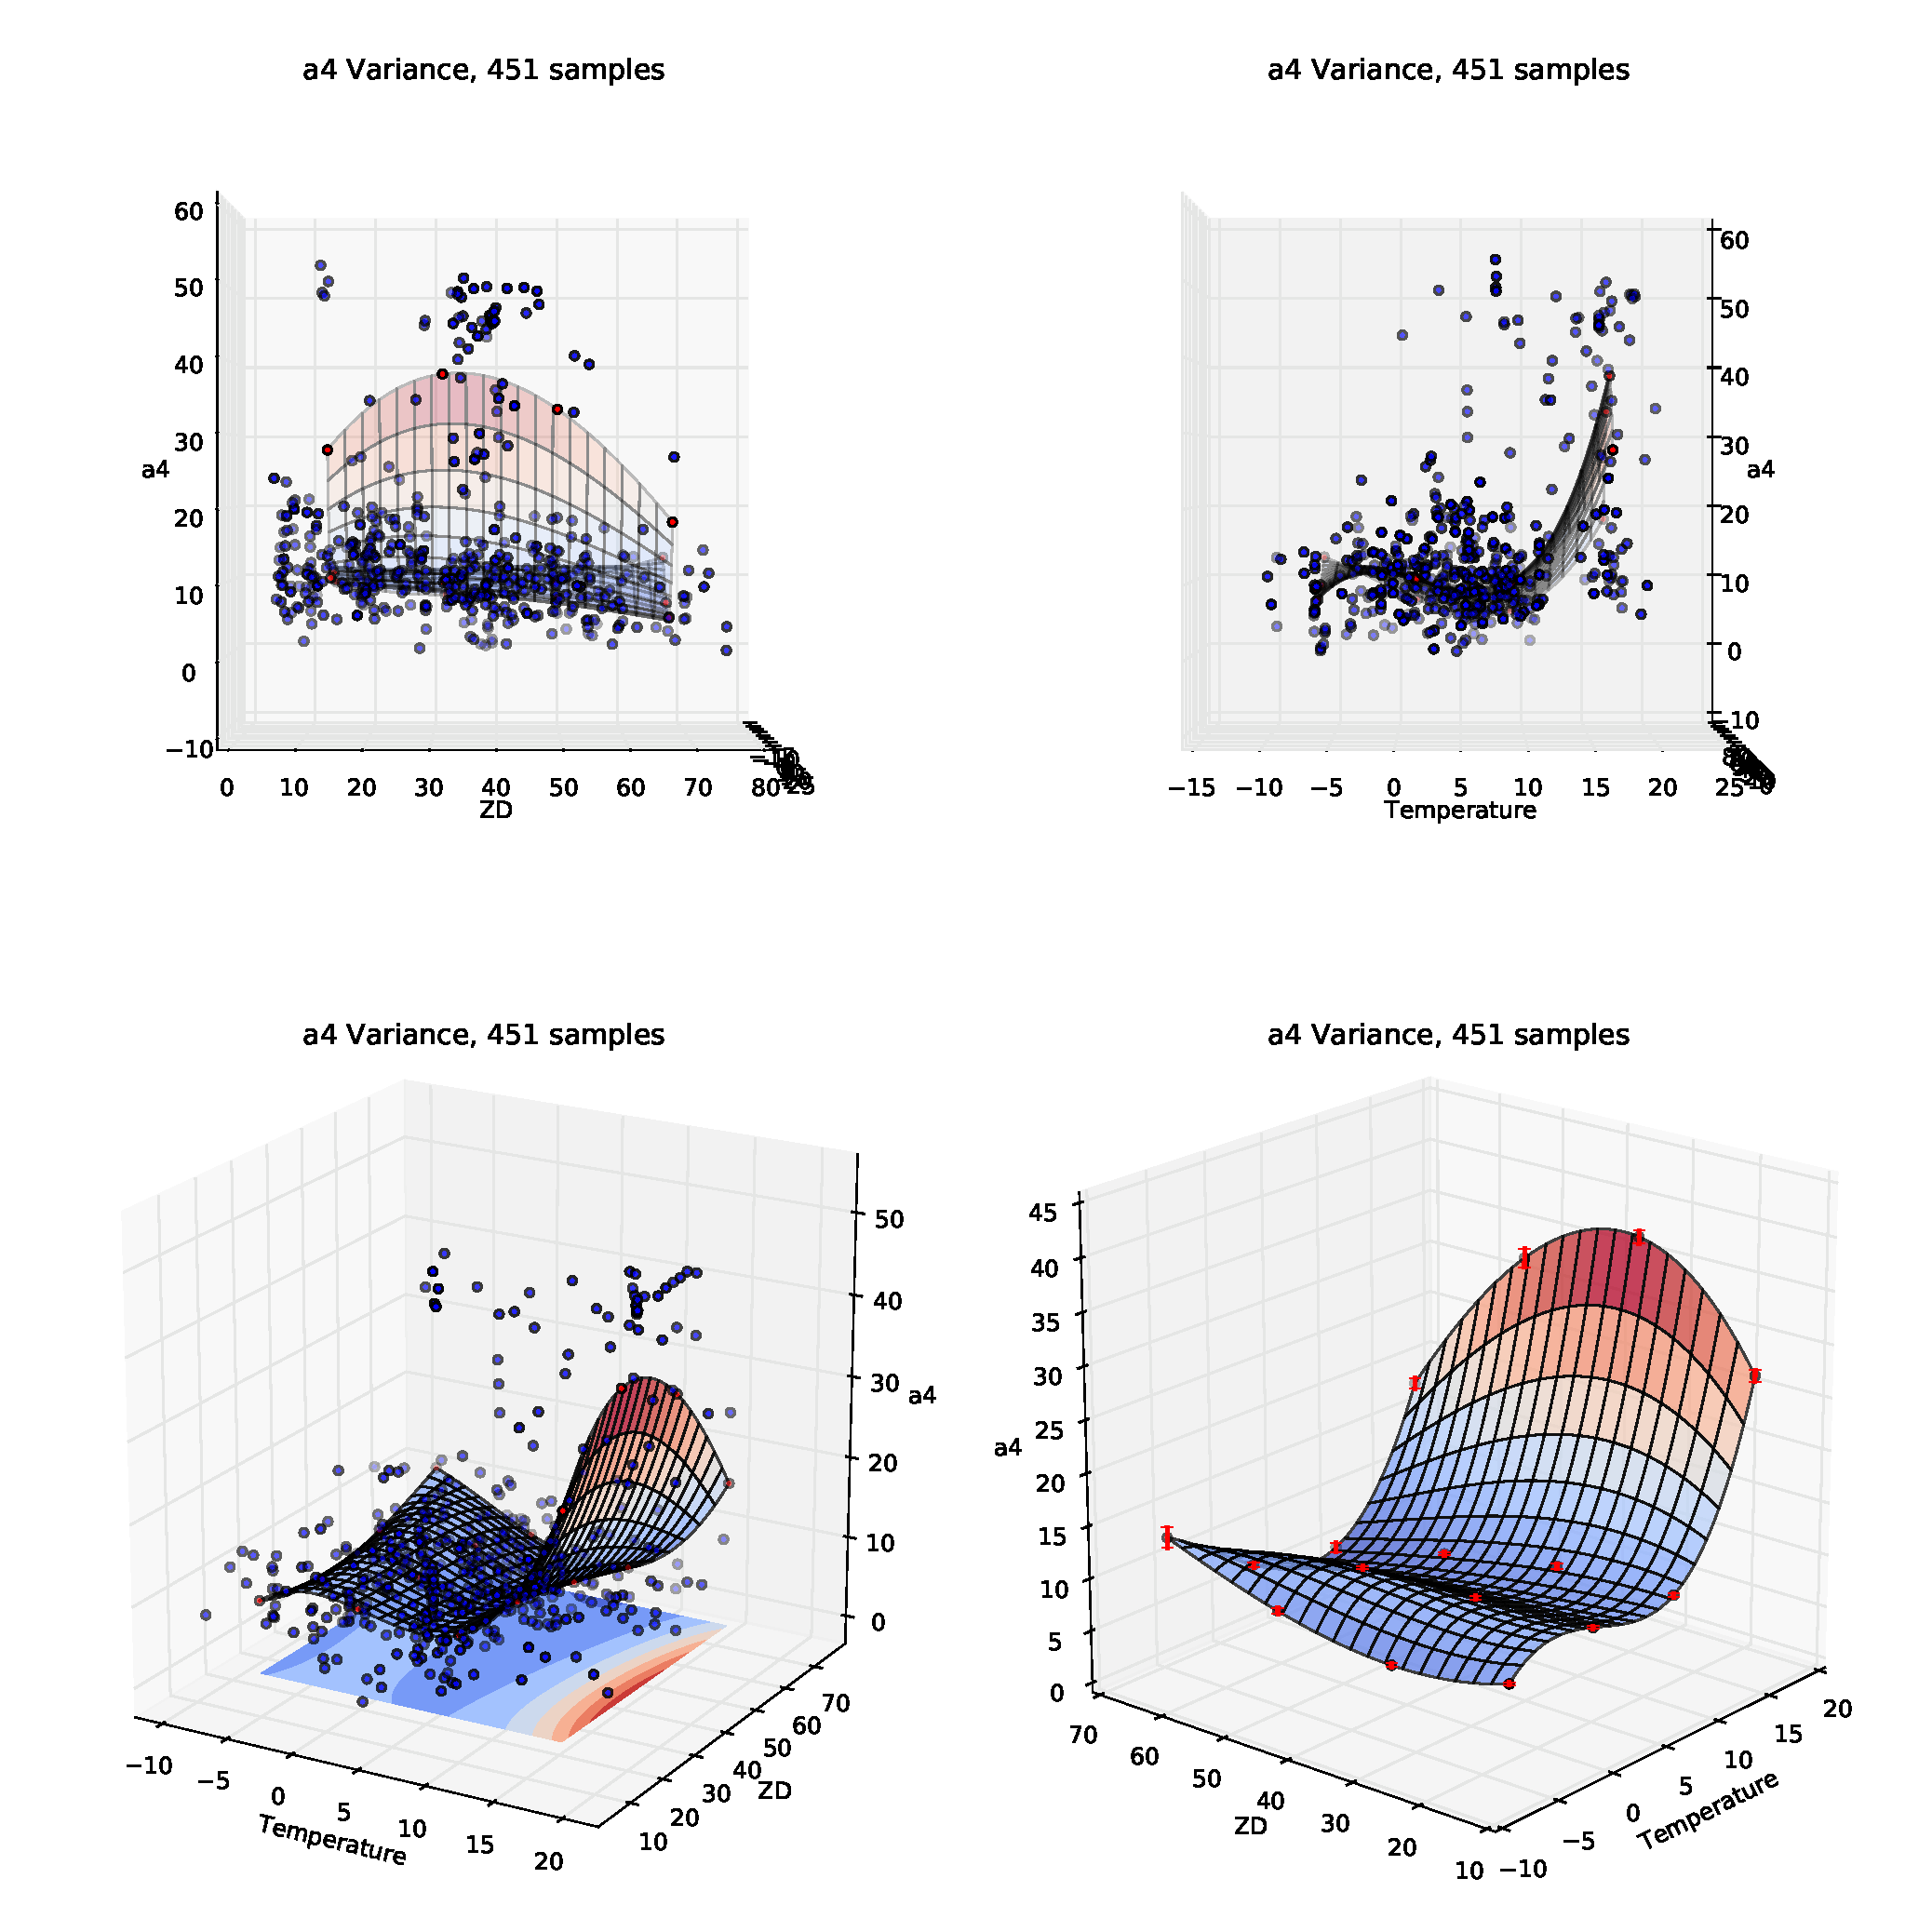
\includegraphics[scale=.48]{psf_surf/a4_var.pdf}
	\caption[Varianz Temperatur- und Elevationsabhängigkeit von $A_4$]{Varianz Temperatur- und Elevationsabhängigkeit von $A_4$. Es liegen 451 Fokusaufnahmen zugrunde, die jeweils einem blauen Punkt entsprechen. Die Plots oben links und rechts entsprechen der Projektion auf die Temperatur- und Elevations-Achse respektive. Die roten Kontrollpunkt wurden als Durchschnittswerte berechnet (mean). Die roten Balken an den Kontrollpunkten im Plot unten rechts sind ein Maß für die Streuung des Kontrollpunktes. }
    \label{psf_surf_a4_var_inline}
\end{figure}

\section{Zukunftsaussicht}
Die in den Korrelationsmatrizen enthaltene Transinformation kann als ein erster Anhaltspunkt dienen, um weitere Abhängigkeiten der Fokusfunktion aufzudecken oder schädliche Effekte auf die Bildqualität aufzuspüren. Dazu gehört, dass unter Umständen auch auch höhere Momente der PSF-Parameter betrachtet werden und mit den weiteren Freiheitsgraden des Hexapod, der den Sekundärspiegel justiert, korrigiert werden.\\
In Hinblick auf den Defokus sollte aufgrund des geringen Fehlers der Interpolant genauere Ergebnisse als die linear genäherte Fokusfunktion liefern. Weitere Fokusserien, die im Verlauf der Zeit aufgenommen werden, können die Genauigkeit des Interpolanten sogar erhöhen. Der Idealfall wäre eine Fokusfunktion, die alle Abhängigkeiten berücksichtigt, die zu einem Driften des Fokus führen und diese automatisch in einem ersten Schritt korrigiert, so dass eine Serie von Fokusaufnahmen gar nicht mehr notwendig ist.

  \begin{appendix}


\chapter{Plots}
Eine detaillierte Beschreibung der Herleitung sowie Erläuterung der Begriffe, welche in diesen Plots verwendet werden, findet sich in Kapitel \ref{chapter_2}. Die Plots stehen auch online im PDF-Format zur Verfügung und können so bei bedarf vergrößert betrachtet werden.
\begin{mdframed}[style=emphasis]
	\centering
	\url{http://homepages.physik.uni-muenchen.de/~Jean.Elsner/focus-series/plots/}
\end{mdframed}
\vfill\,

\section{PSF-Verteilungen}
\label{psf_dists}

\begin{figure}[H]
	\centering
	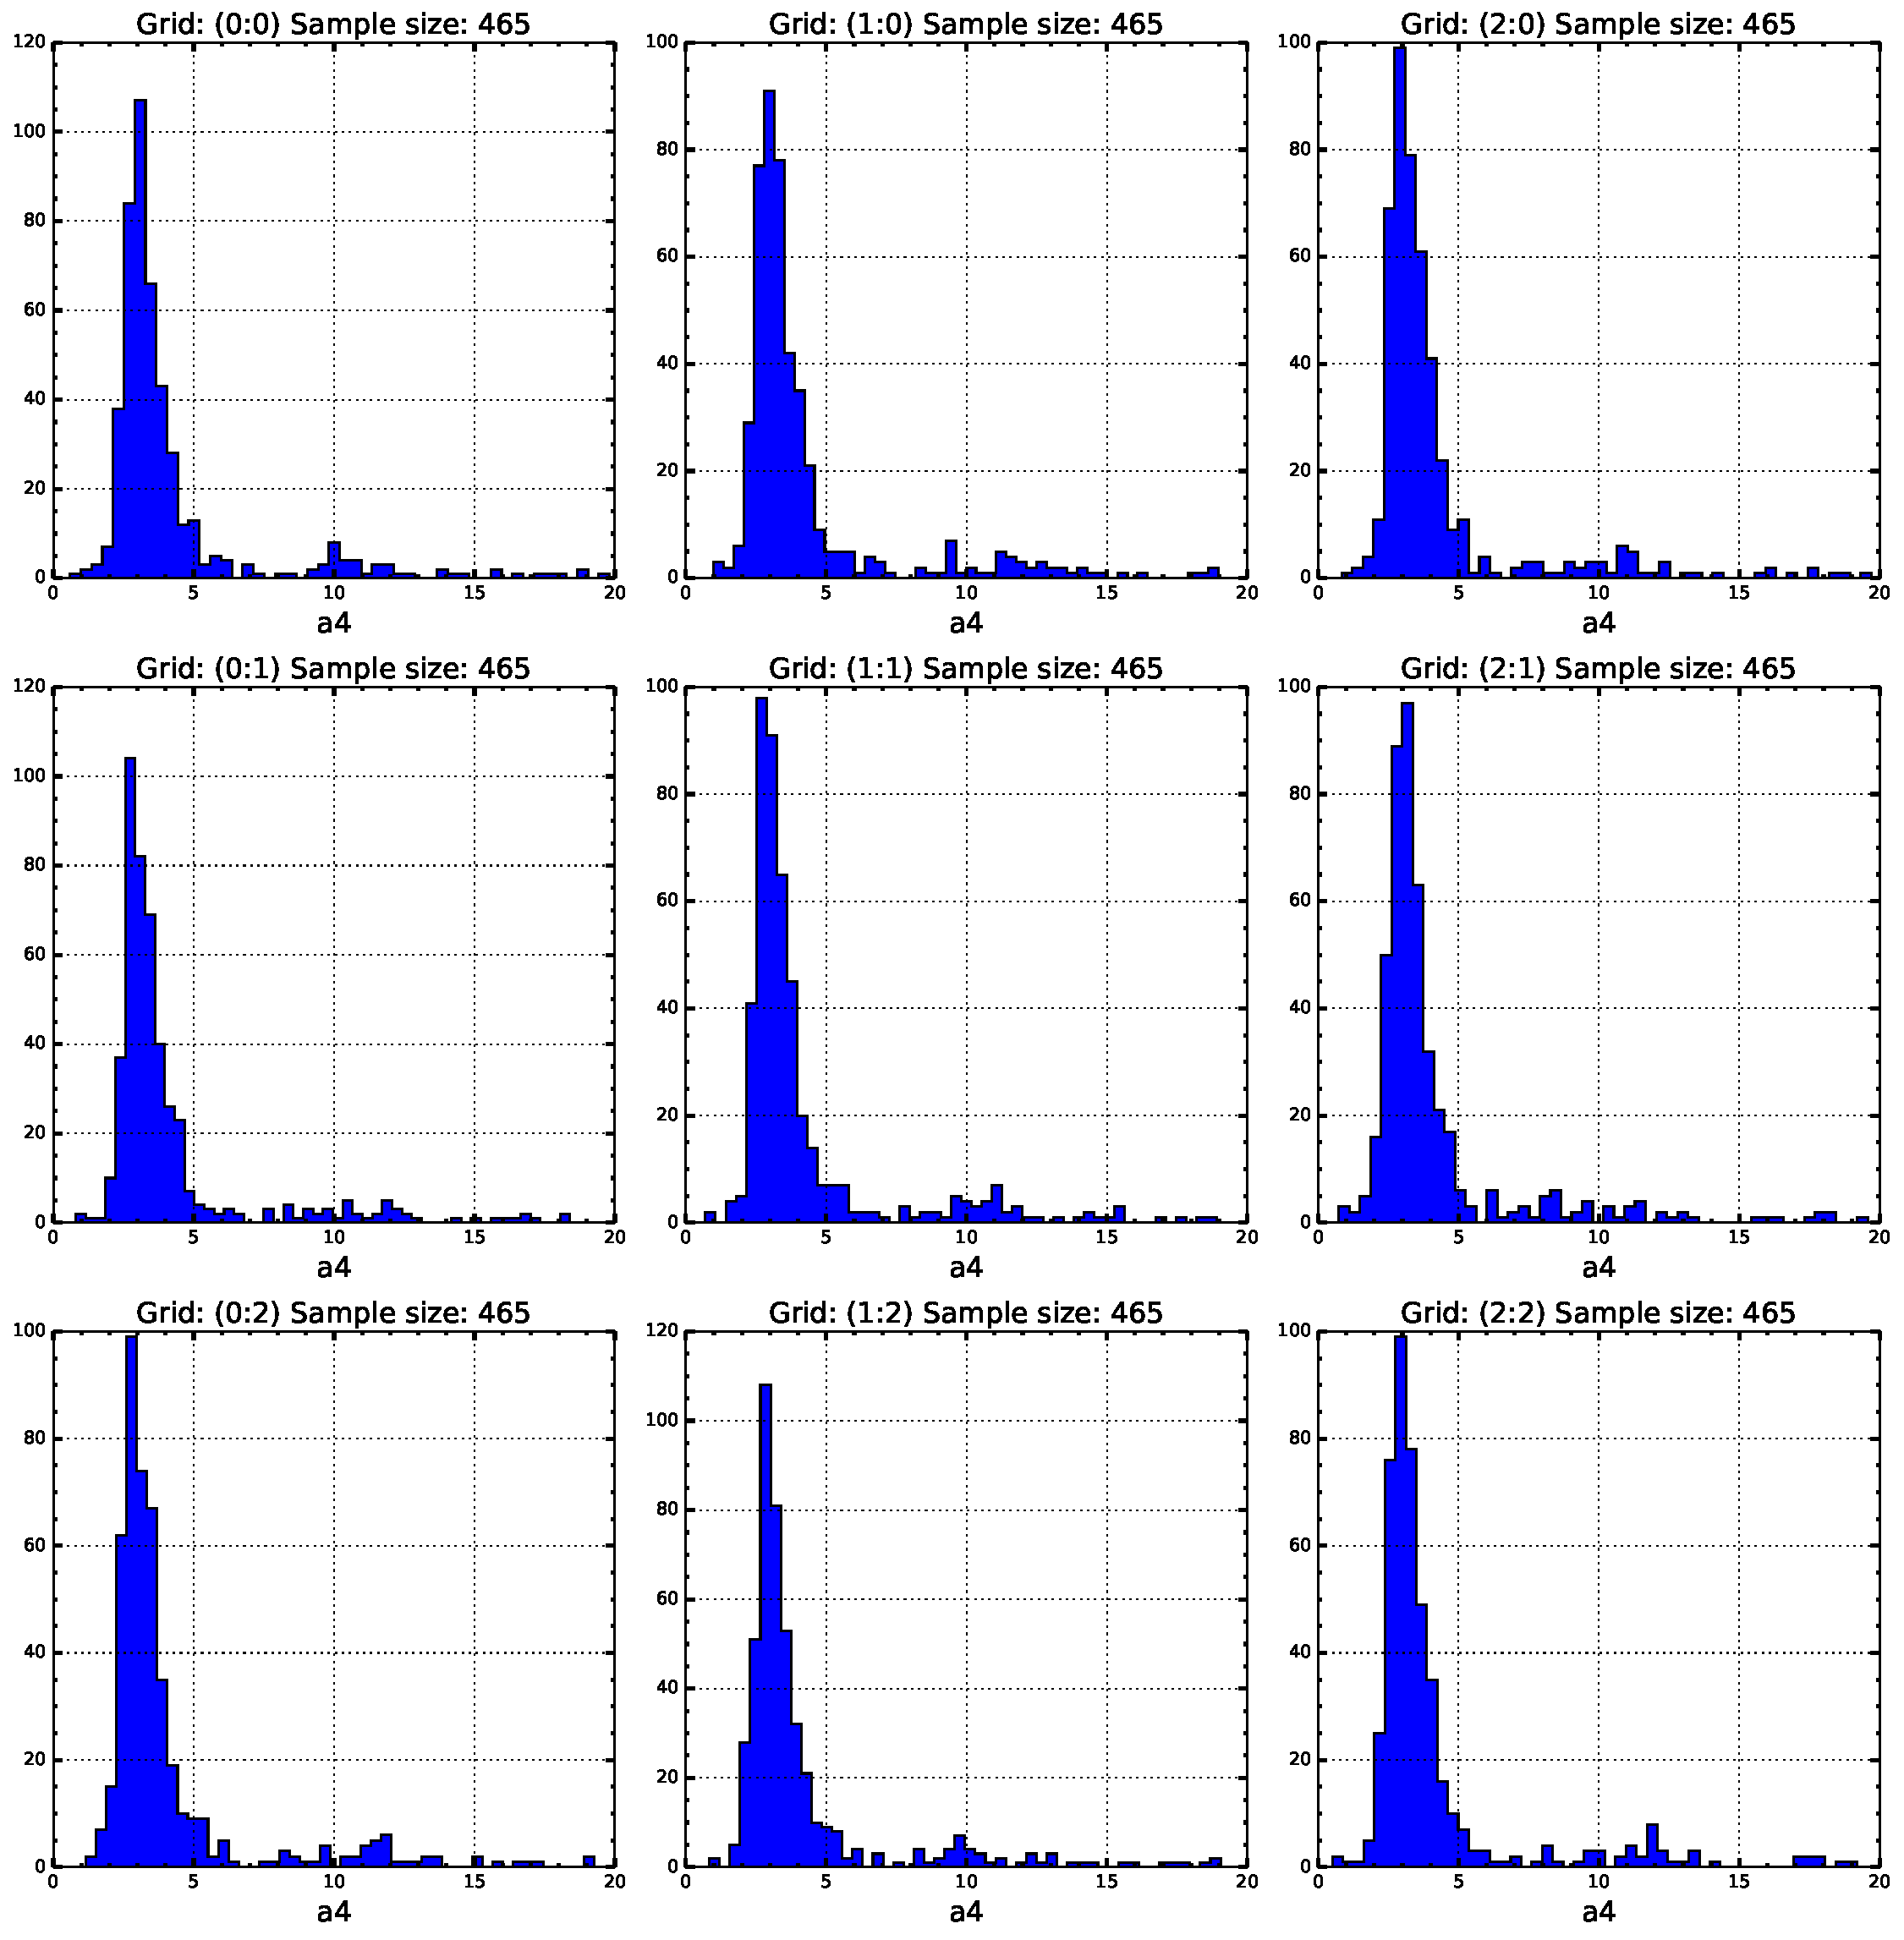
\includegraphics[scale=.42]{psf_dist/a4.pdf}
	\caption[Histogram der Verteilung des PSF-Parameters $A_4$]{Histogram der Verteilung des PSF-Parameters $A_4$}
    \label{psf_dist_a4}
\end{figure}
\begin{figure}[H]
	\centering
	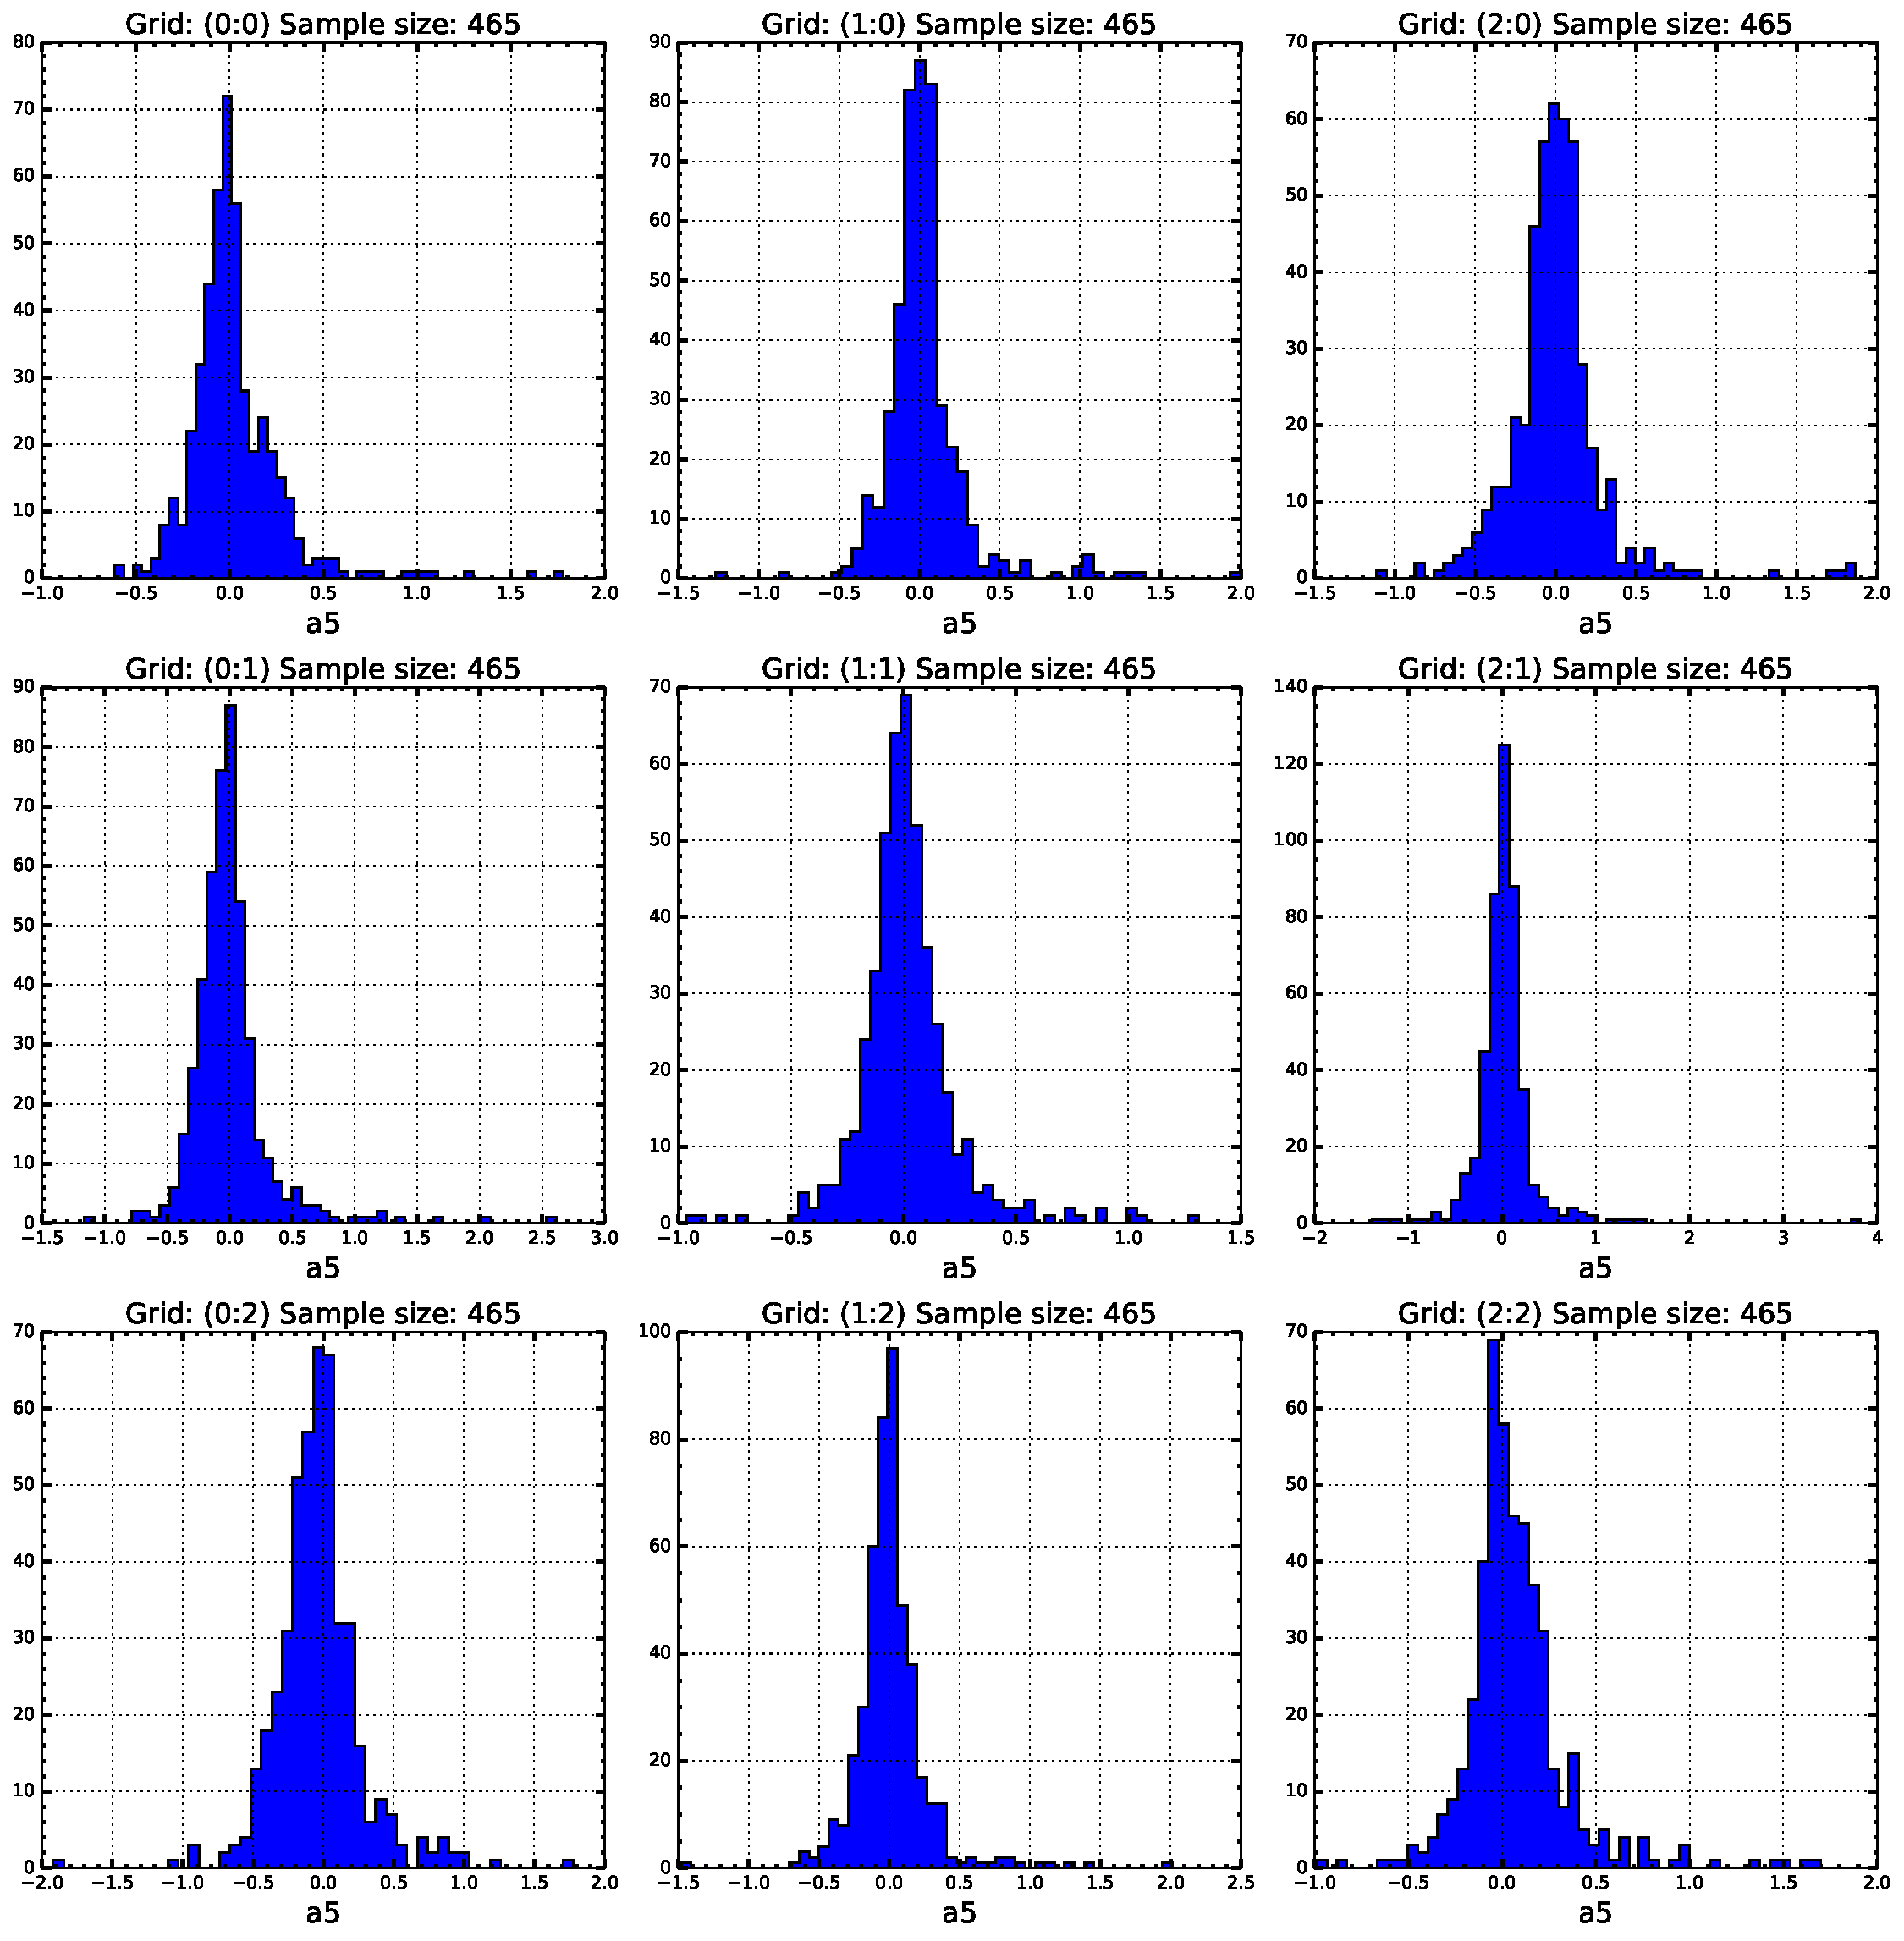
\includegraphics[scale=.42]{psf_dist/a5.pdf}
	\caption[Histogram der Verteilung des PSF-Parameters $A_5$]{Histogram der Verteilung des PSF-Parameters $A_5$}
    \label{psf_dist_a5}
\end{figure}
\begin{figure}[H]
	\centering
	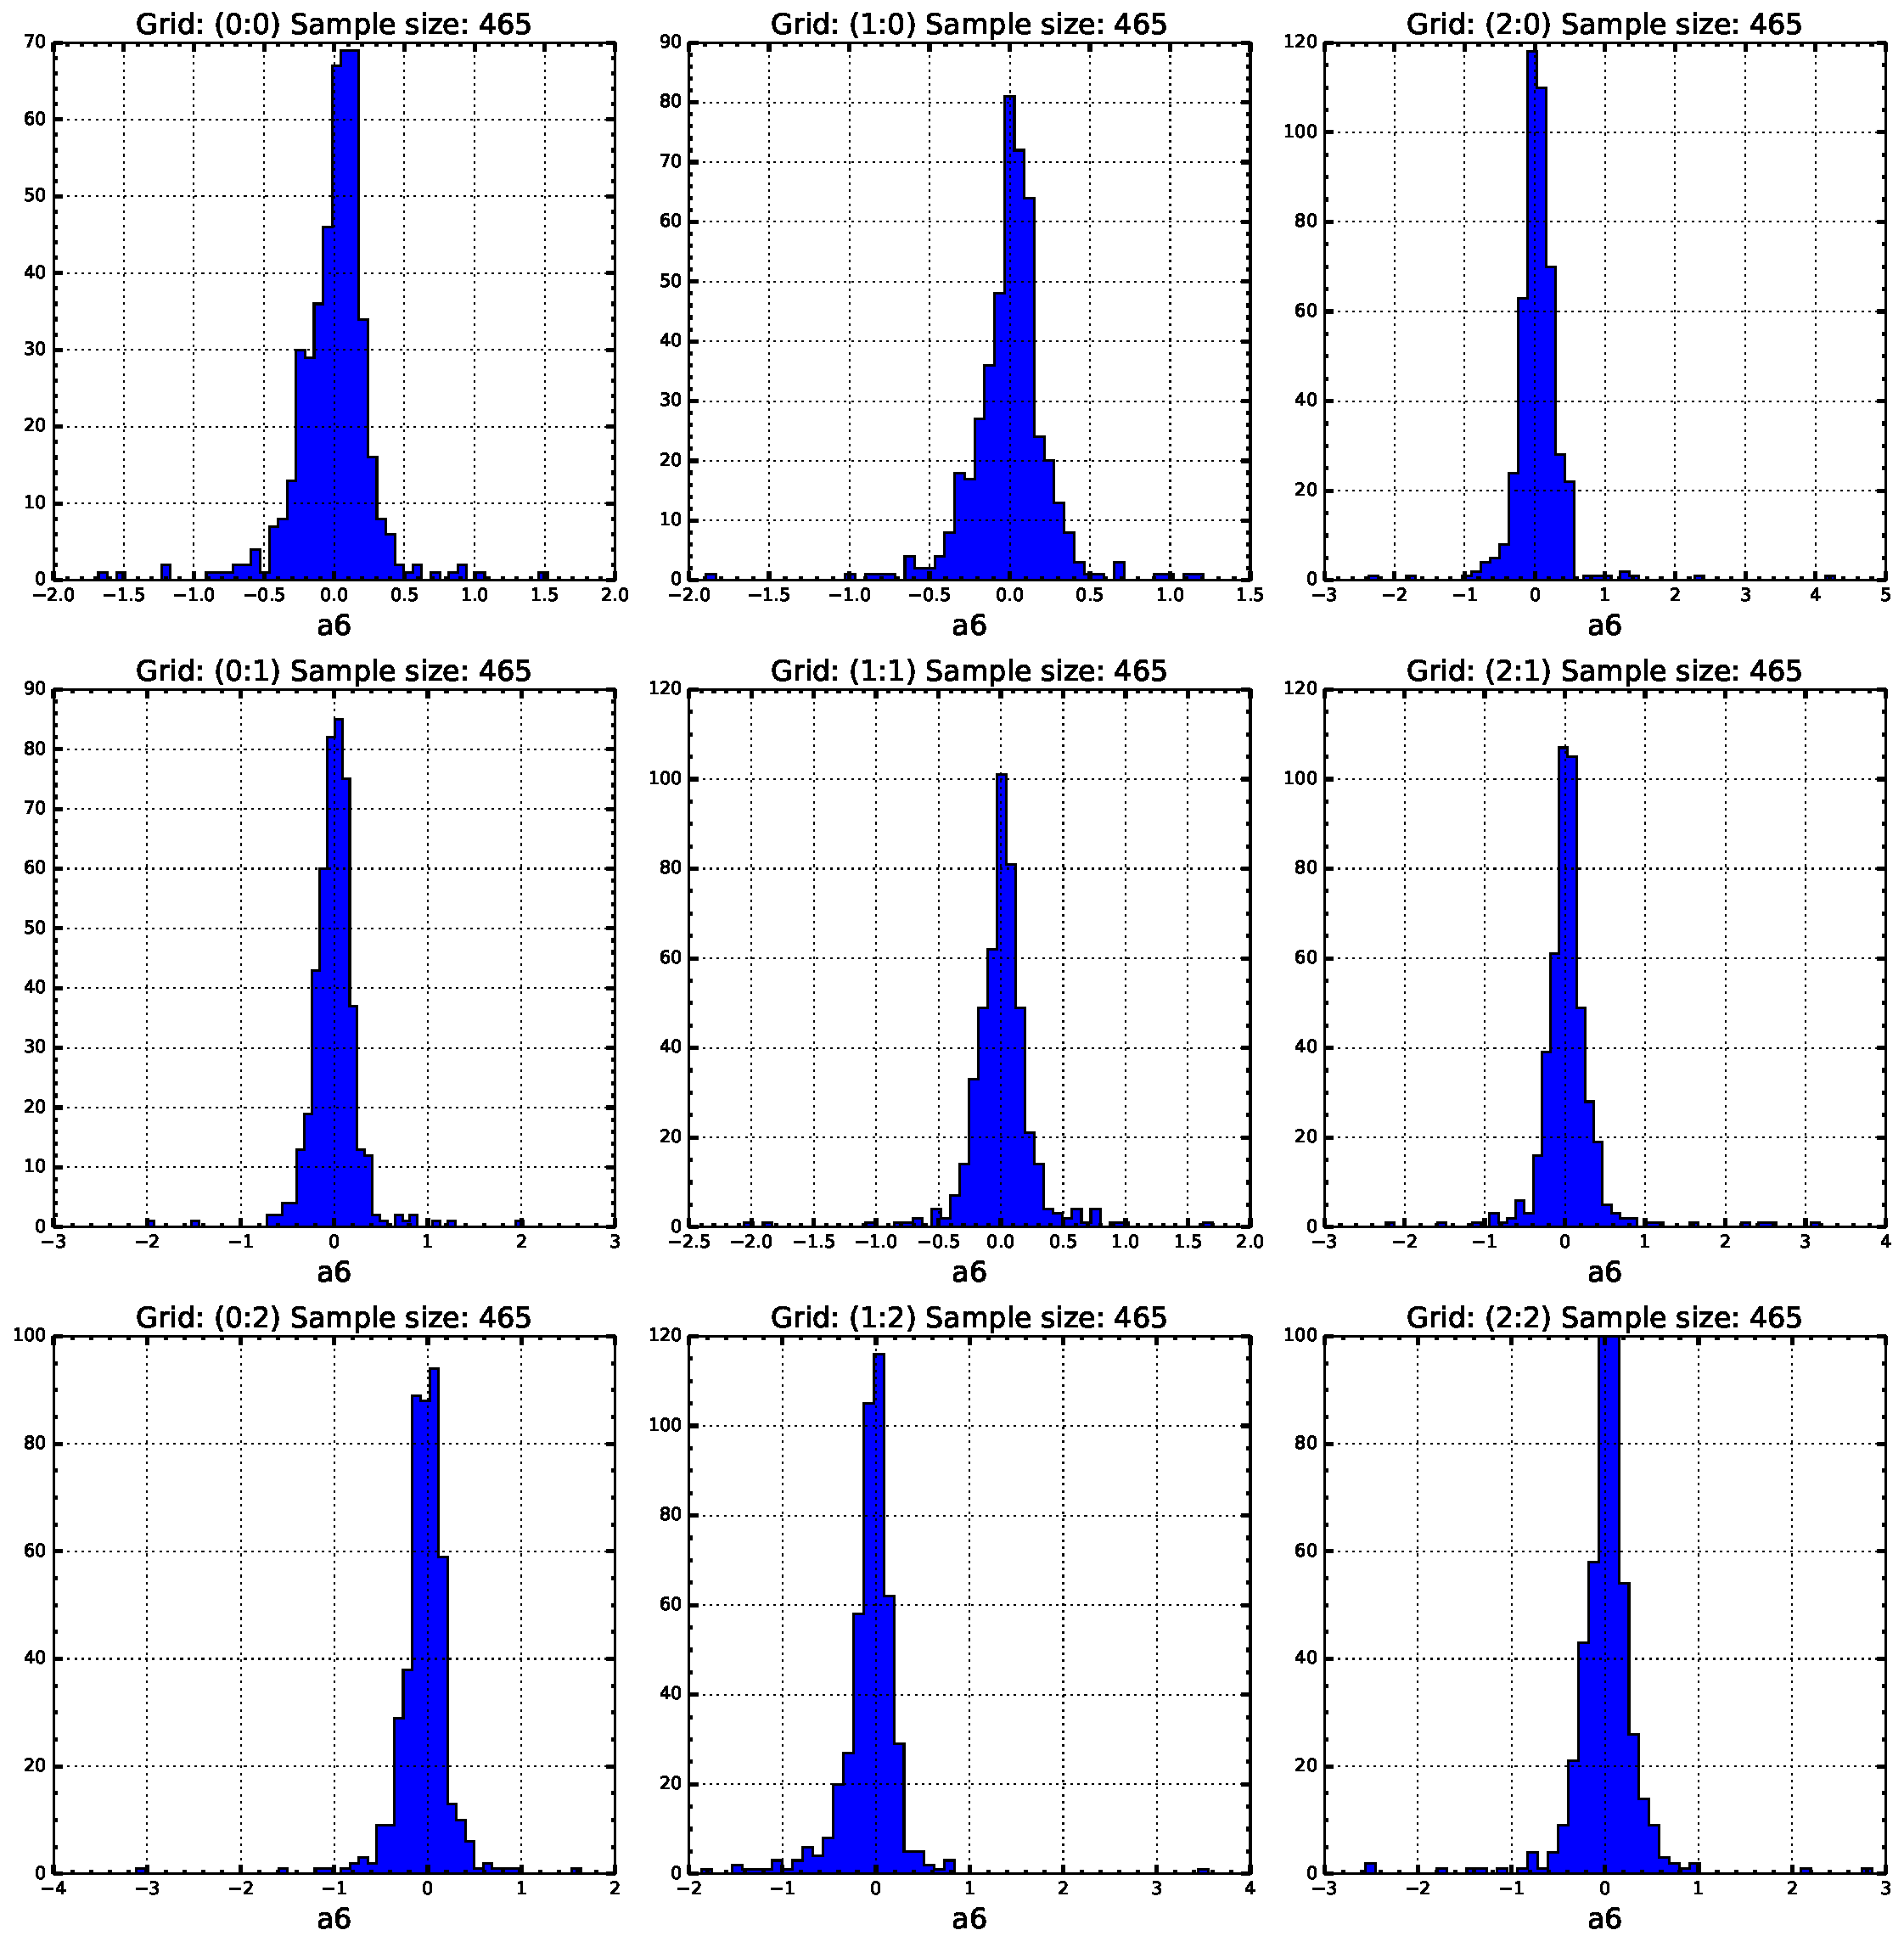
\includegraphics[scale=.42]{psf_dist/a6.pdf}
	\caption[Histogram der Verteilung des PSF-Parameters $A_6$]{Histogram der Verteilung des PSF-Parameters $A_6$}
    \label{psf_dist_a6}
\end{figure}

\section{PSF Temperatur- und Elevationsabhängigkeiten}
\begin{figure}[H]
	\centering
	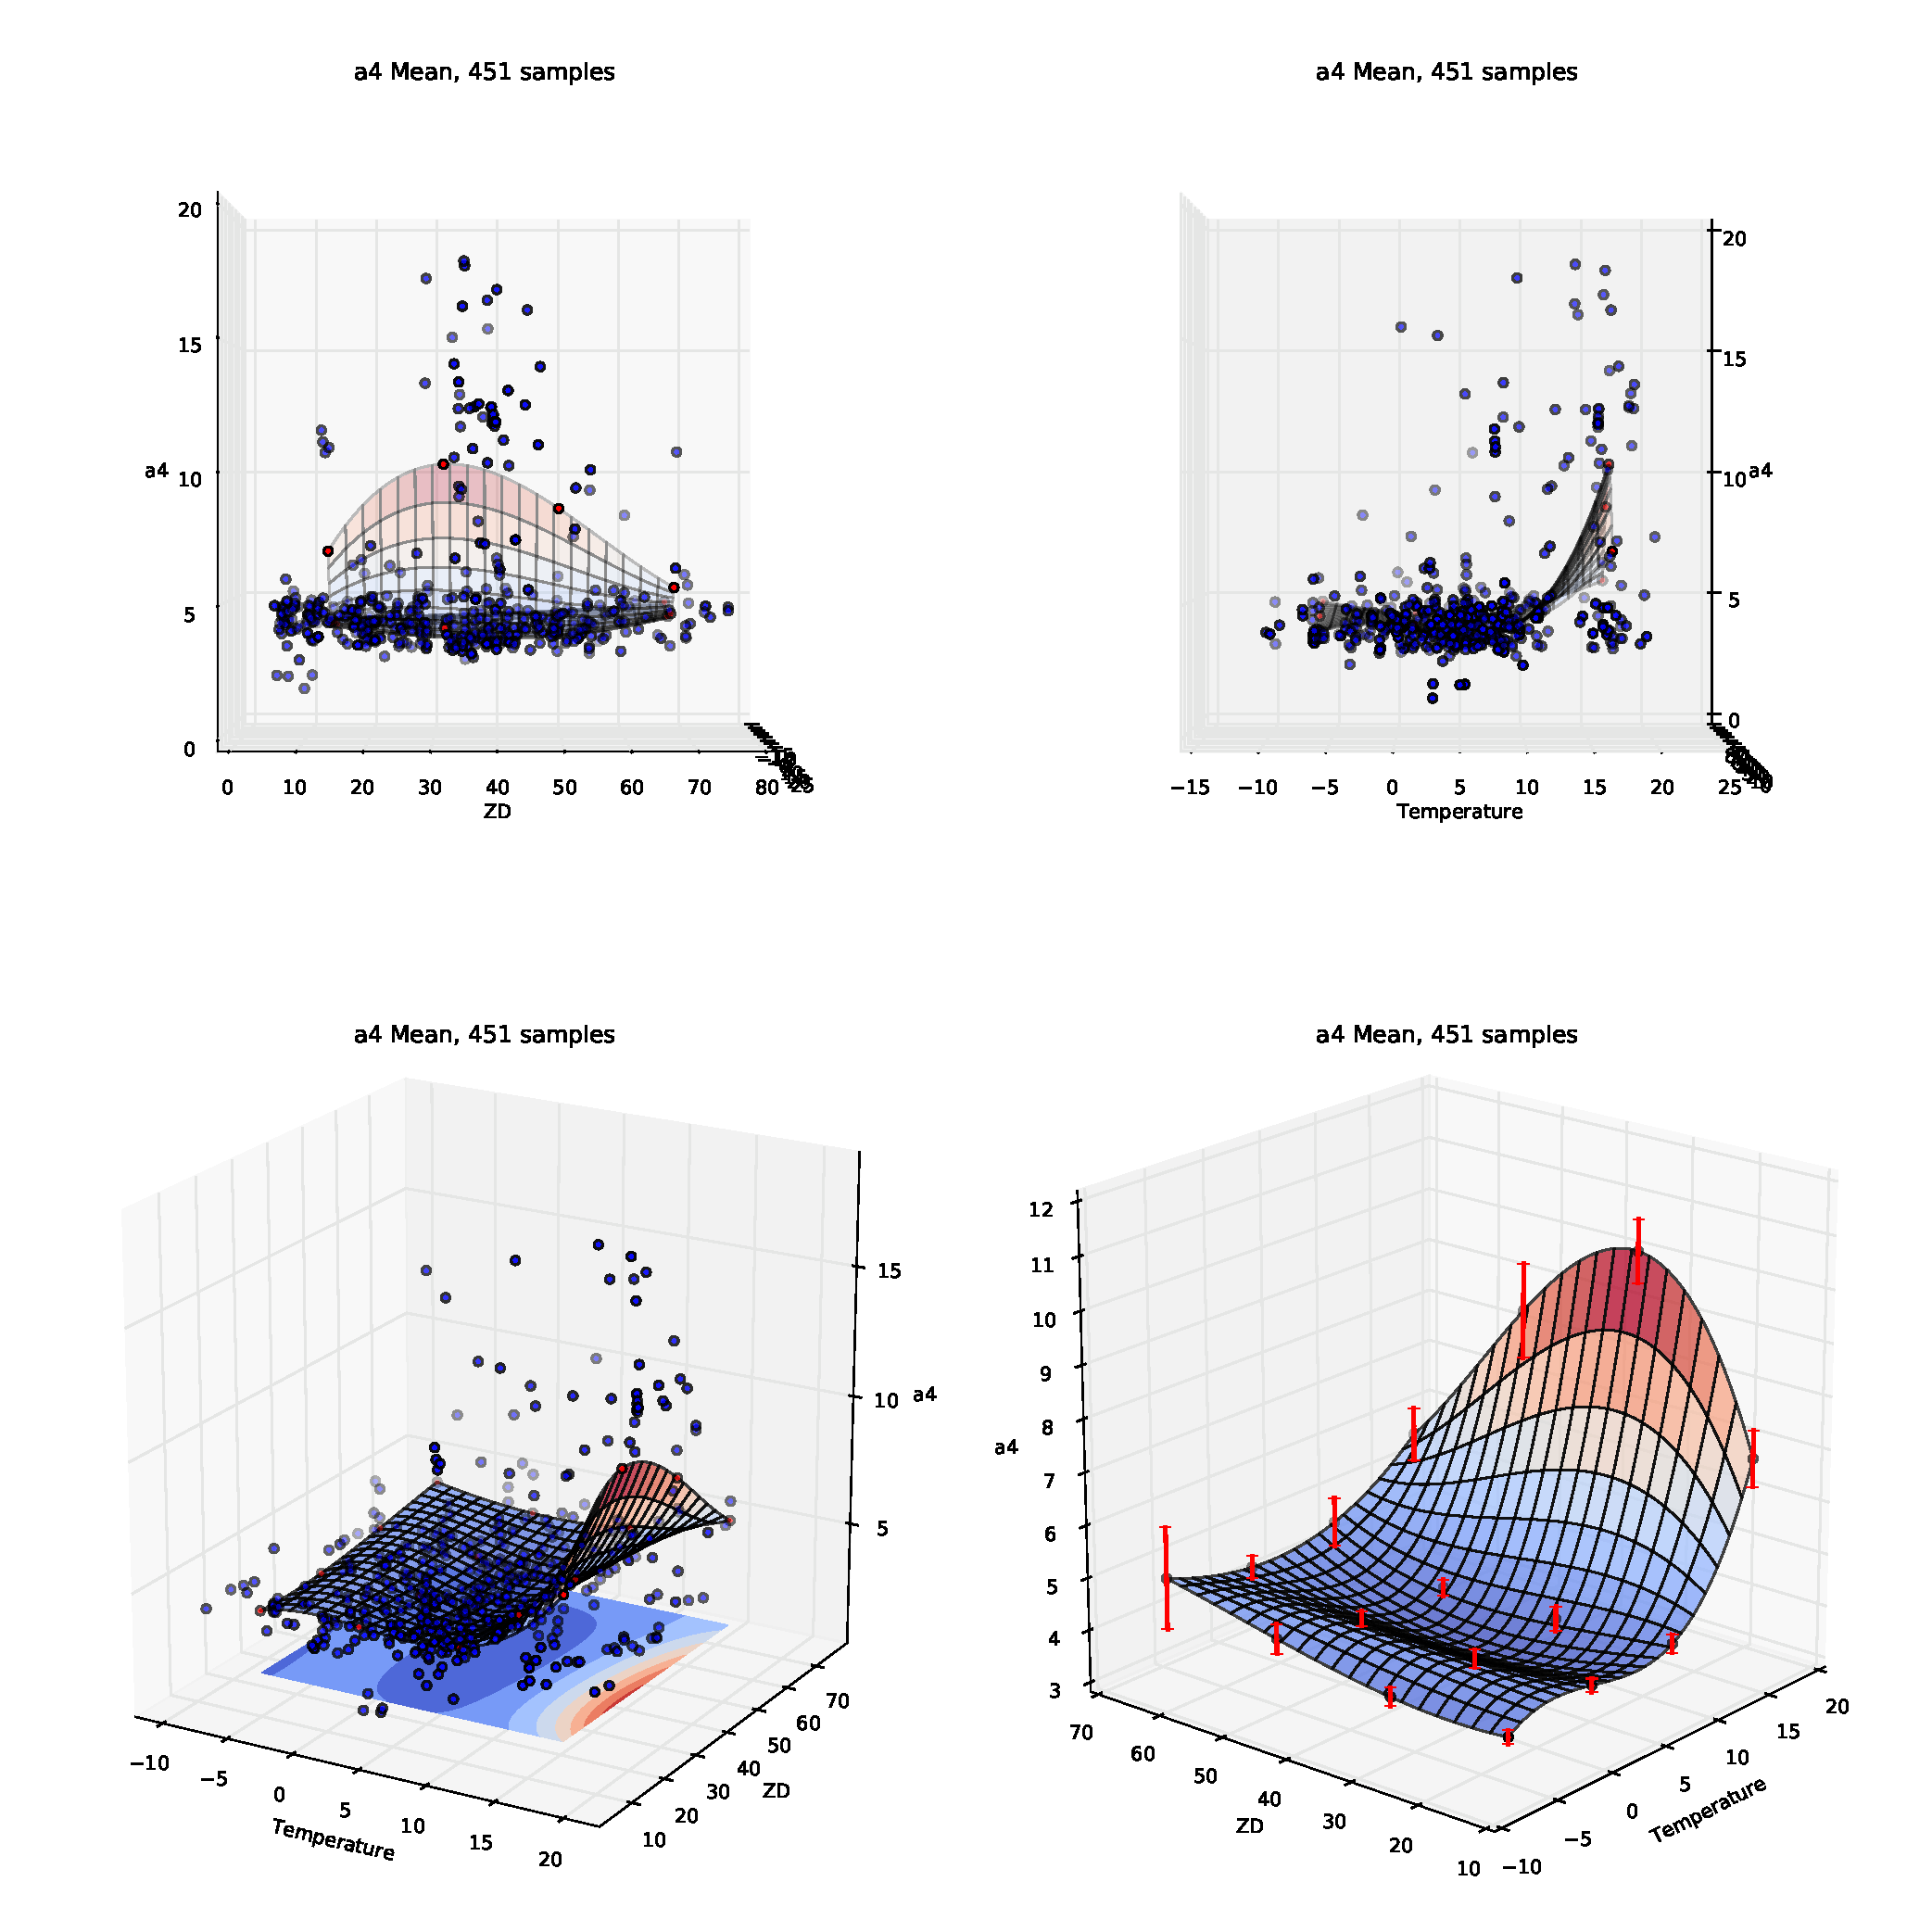
\includegraphics[scale=.48]{psf_surf/a4_mean.pdf}
	\caption[Mean Streu- und Flächenplot des PSF-Parameters $A_4$]{Mean Streu- und Flächenplot des PSF-Parameters $A_4$}
    \label{psf_surf_a4_mean}
\end{figure}
\begin{figure}[H]
	\centering
	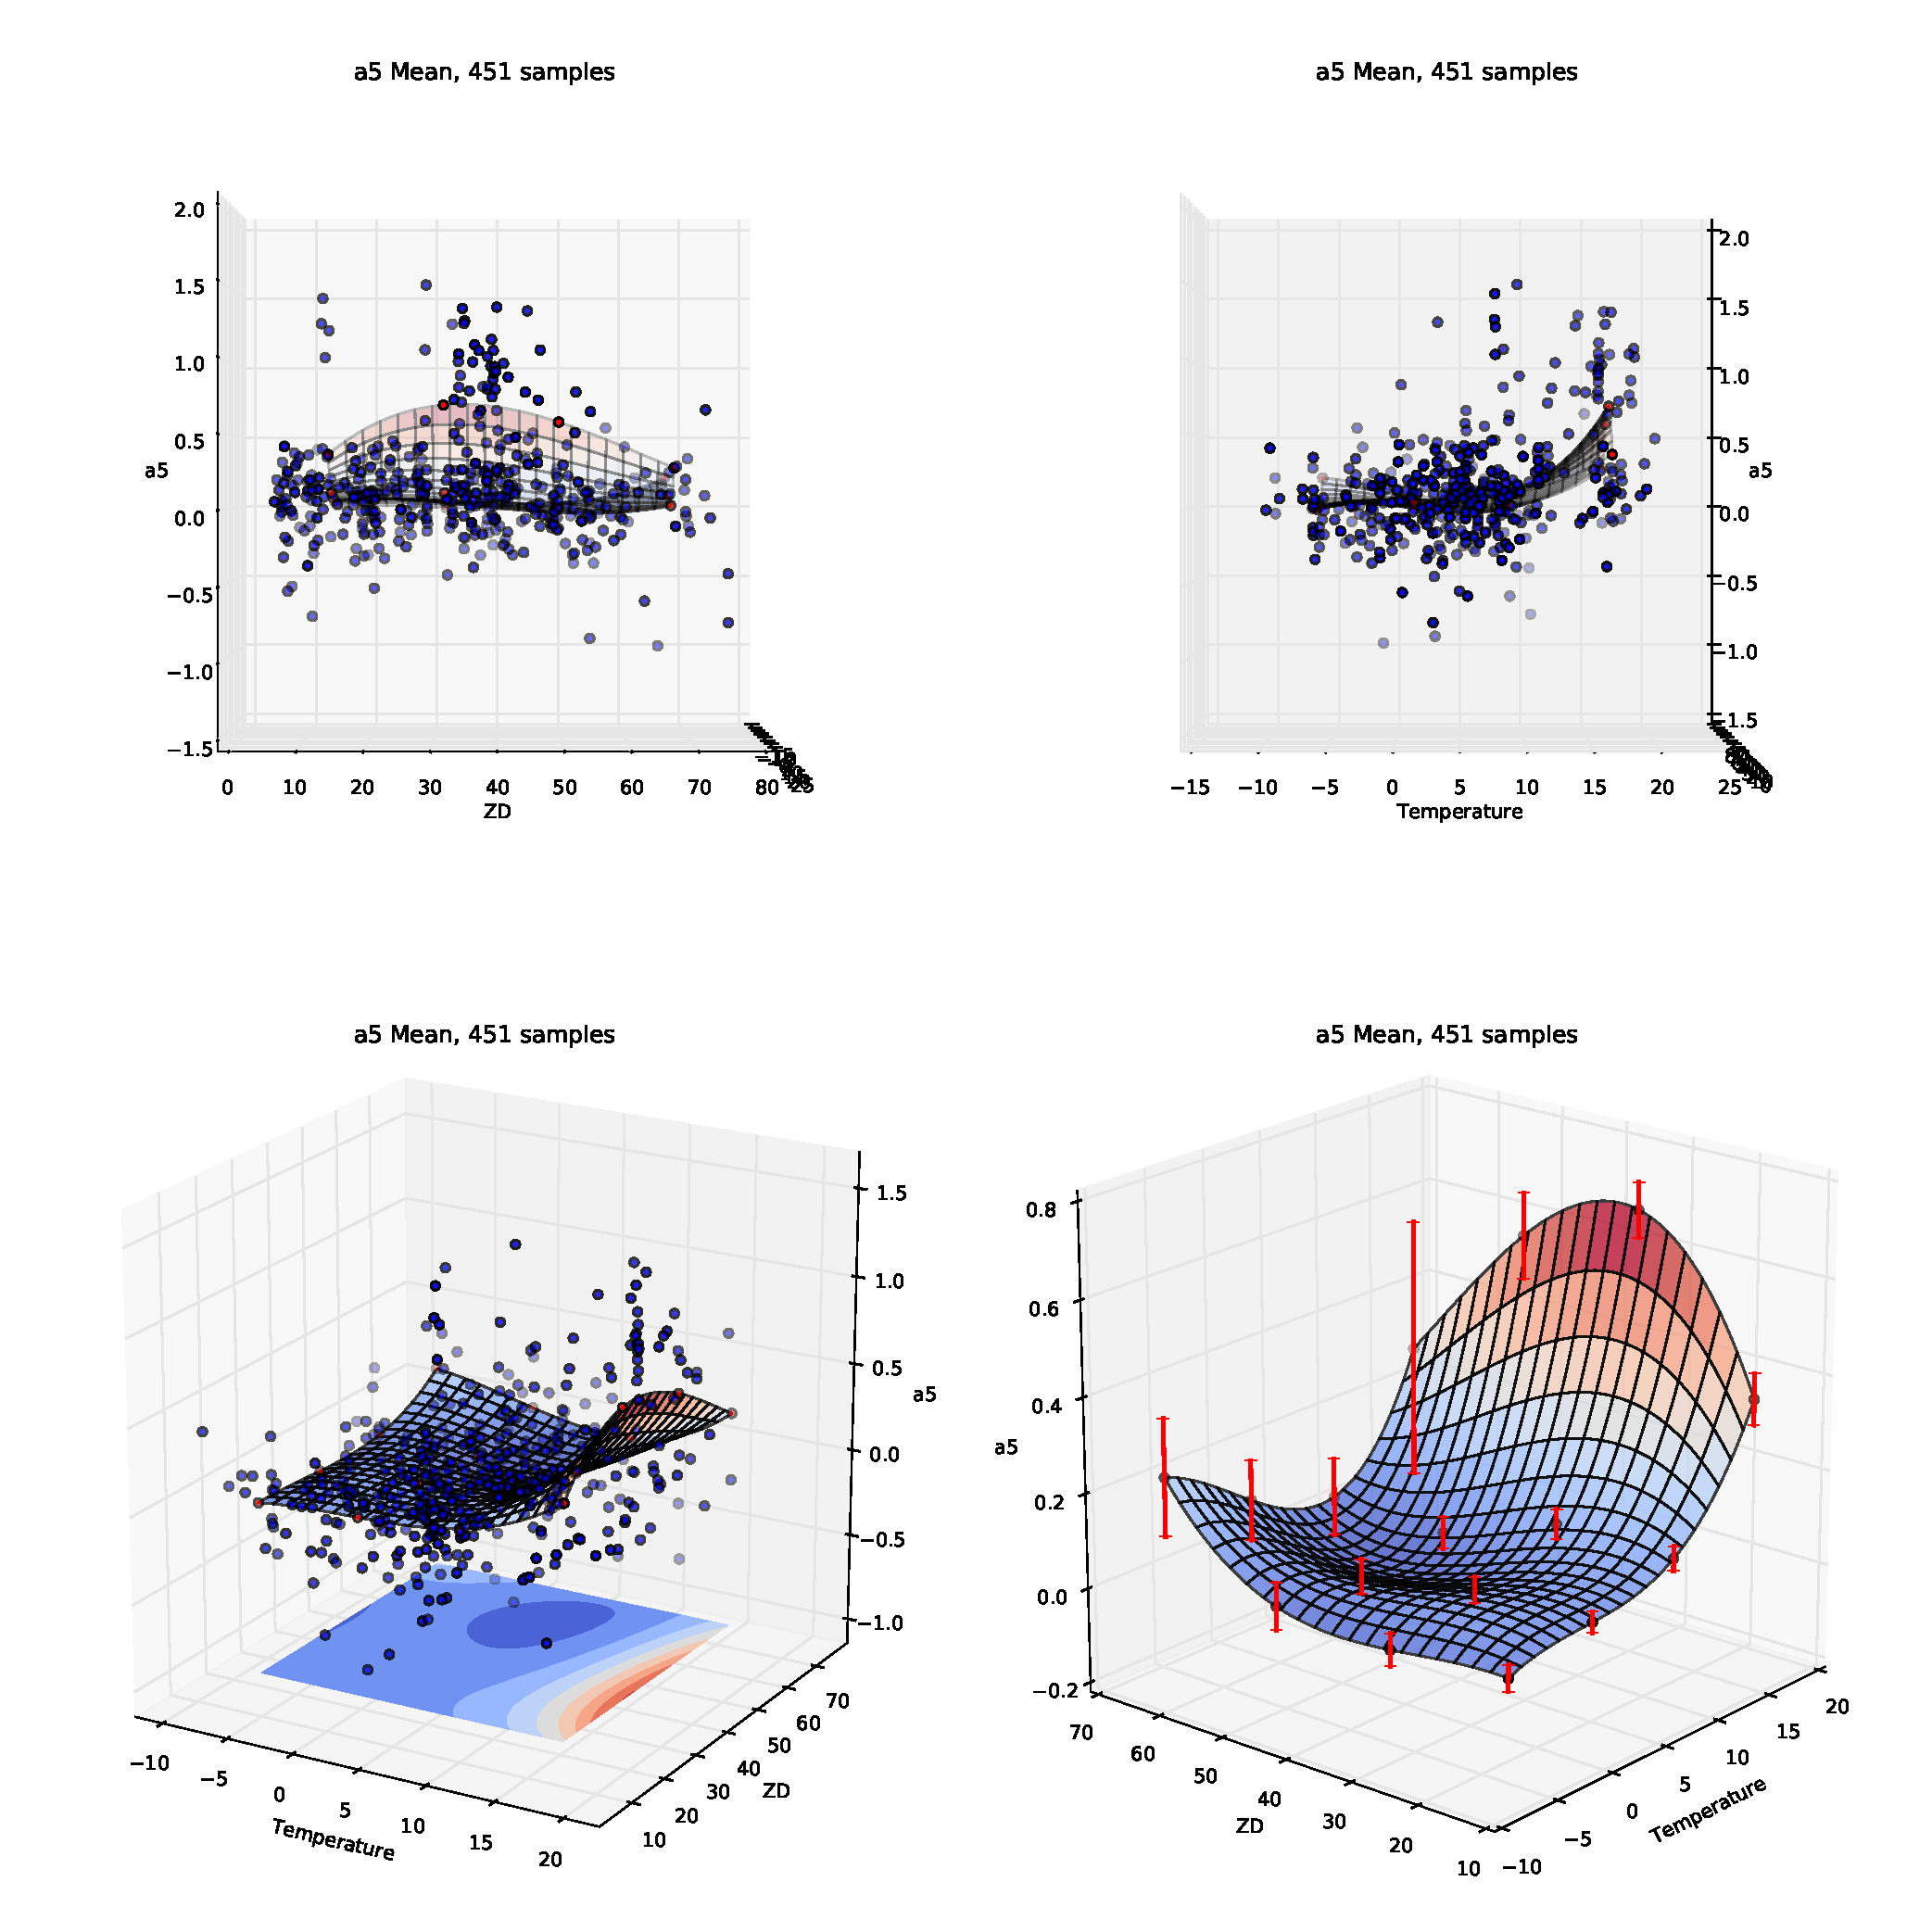
\includegraphics[scale=.48]{psf_surf/a5_mean.pdf}
	\caption[Mean Streu- und Flächenplot des PSF-Parameters $A_5$]{Mean Streu- und Flächenplot des PSF-Parameters $A_5$}
    \label{psf_surf_a5_mean}
\end{figure}
\begin{figure}[H]
	\centering
	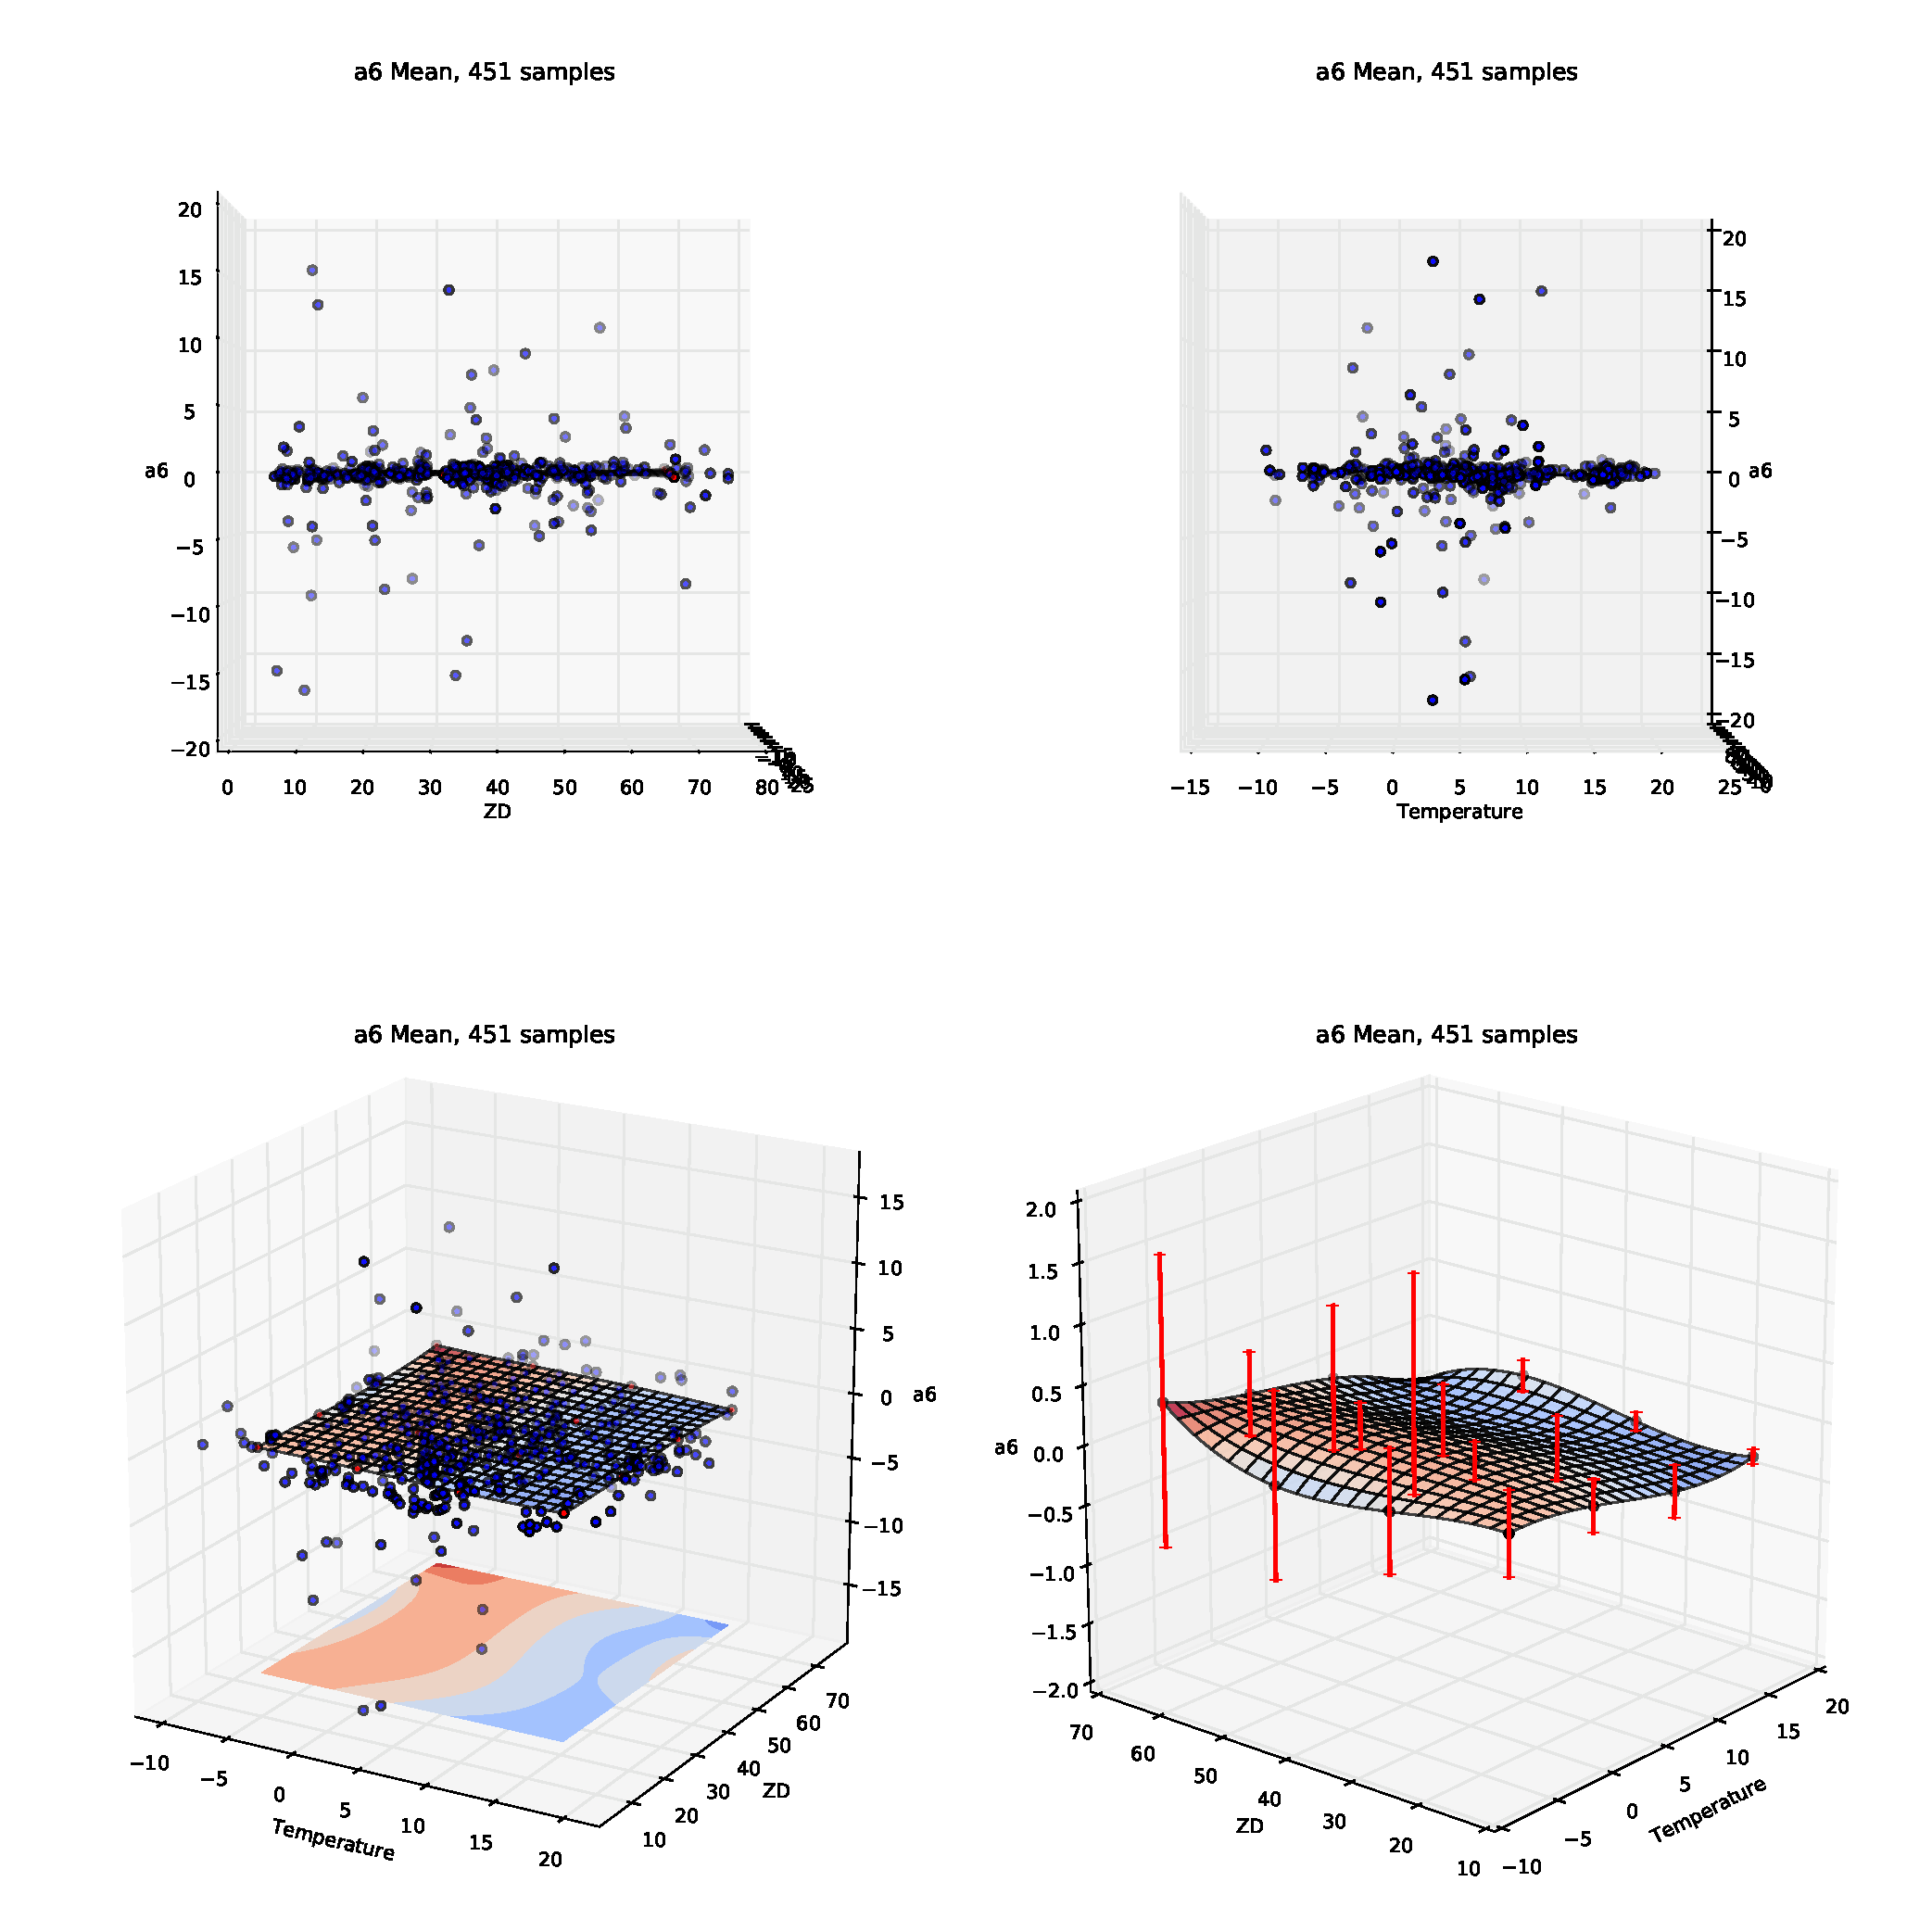
\includegraphics[scale=.48]{psf_surf/a6_mean.pdf}
	\caption[Mean Streu- und Flächenplot des PSF-Parameters $A_6$]{Mean Streu- und Flächenplot des PSF-Parameters $A_6$}
    \label{psf_surf_a6_mean}
\end{figure}

\begin{figure}[H]
	\centering
	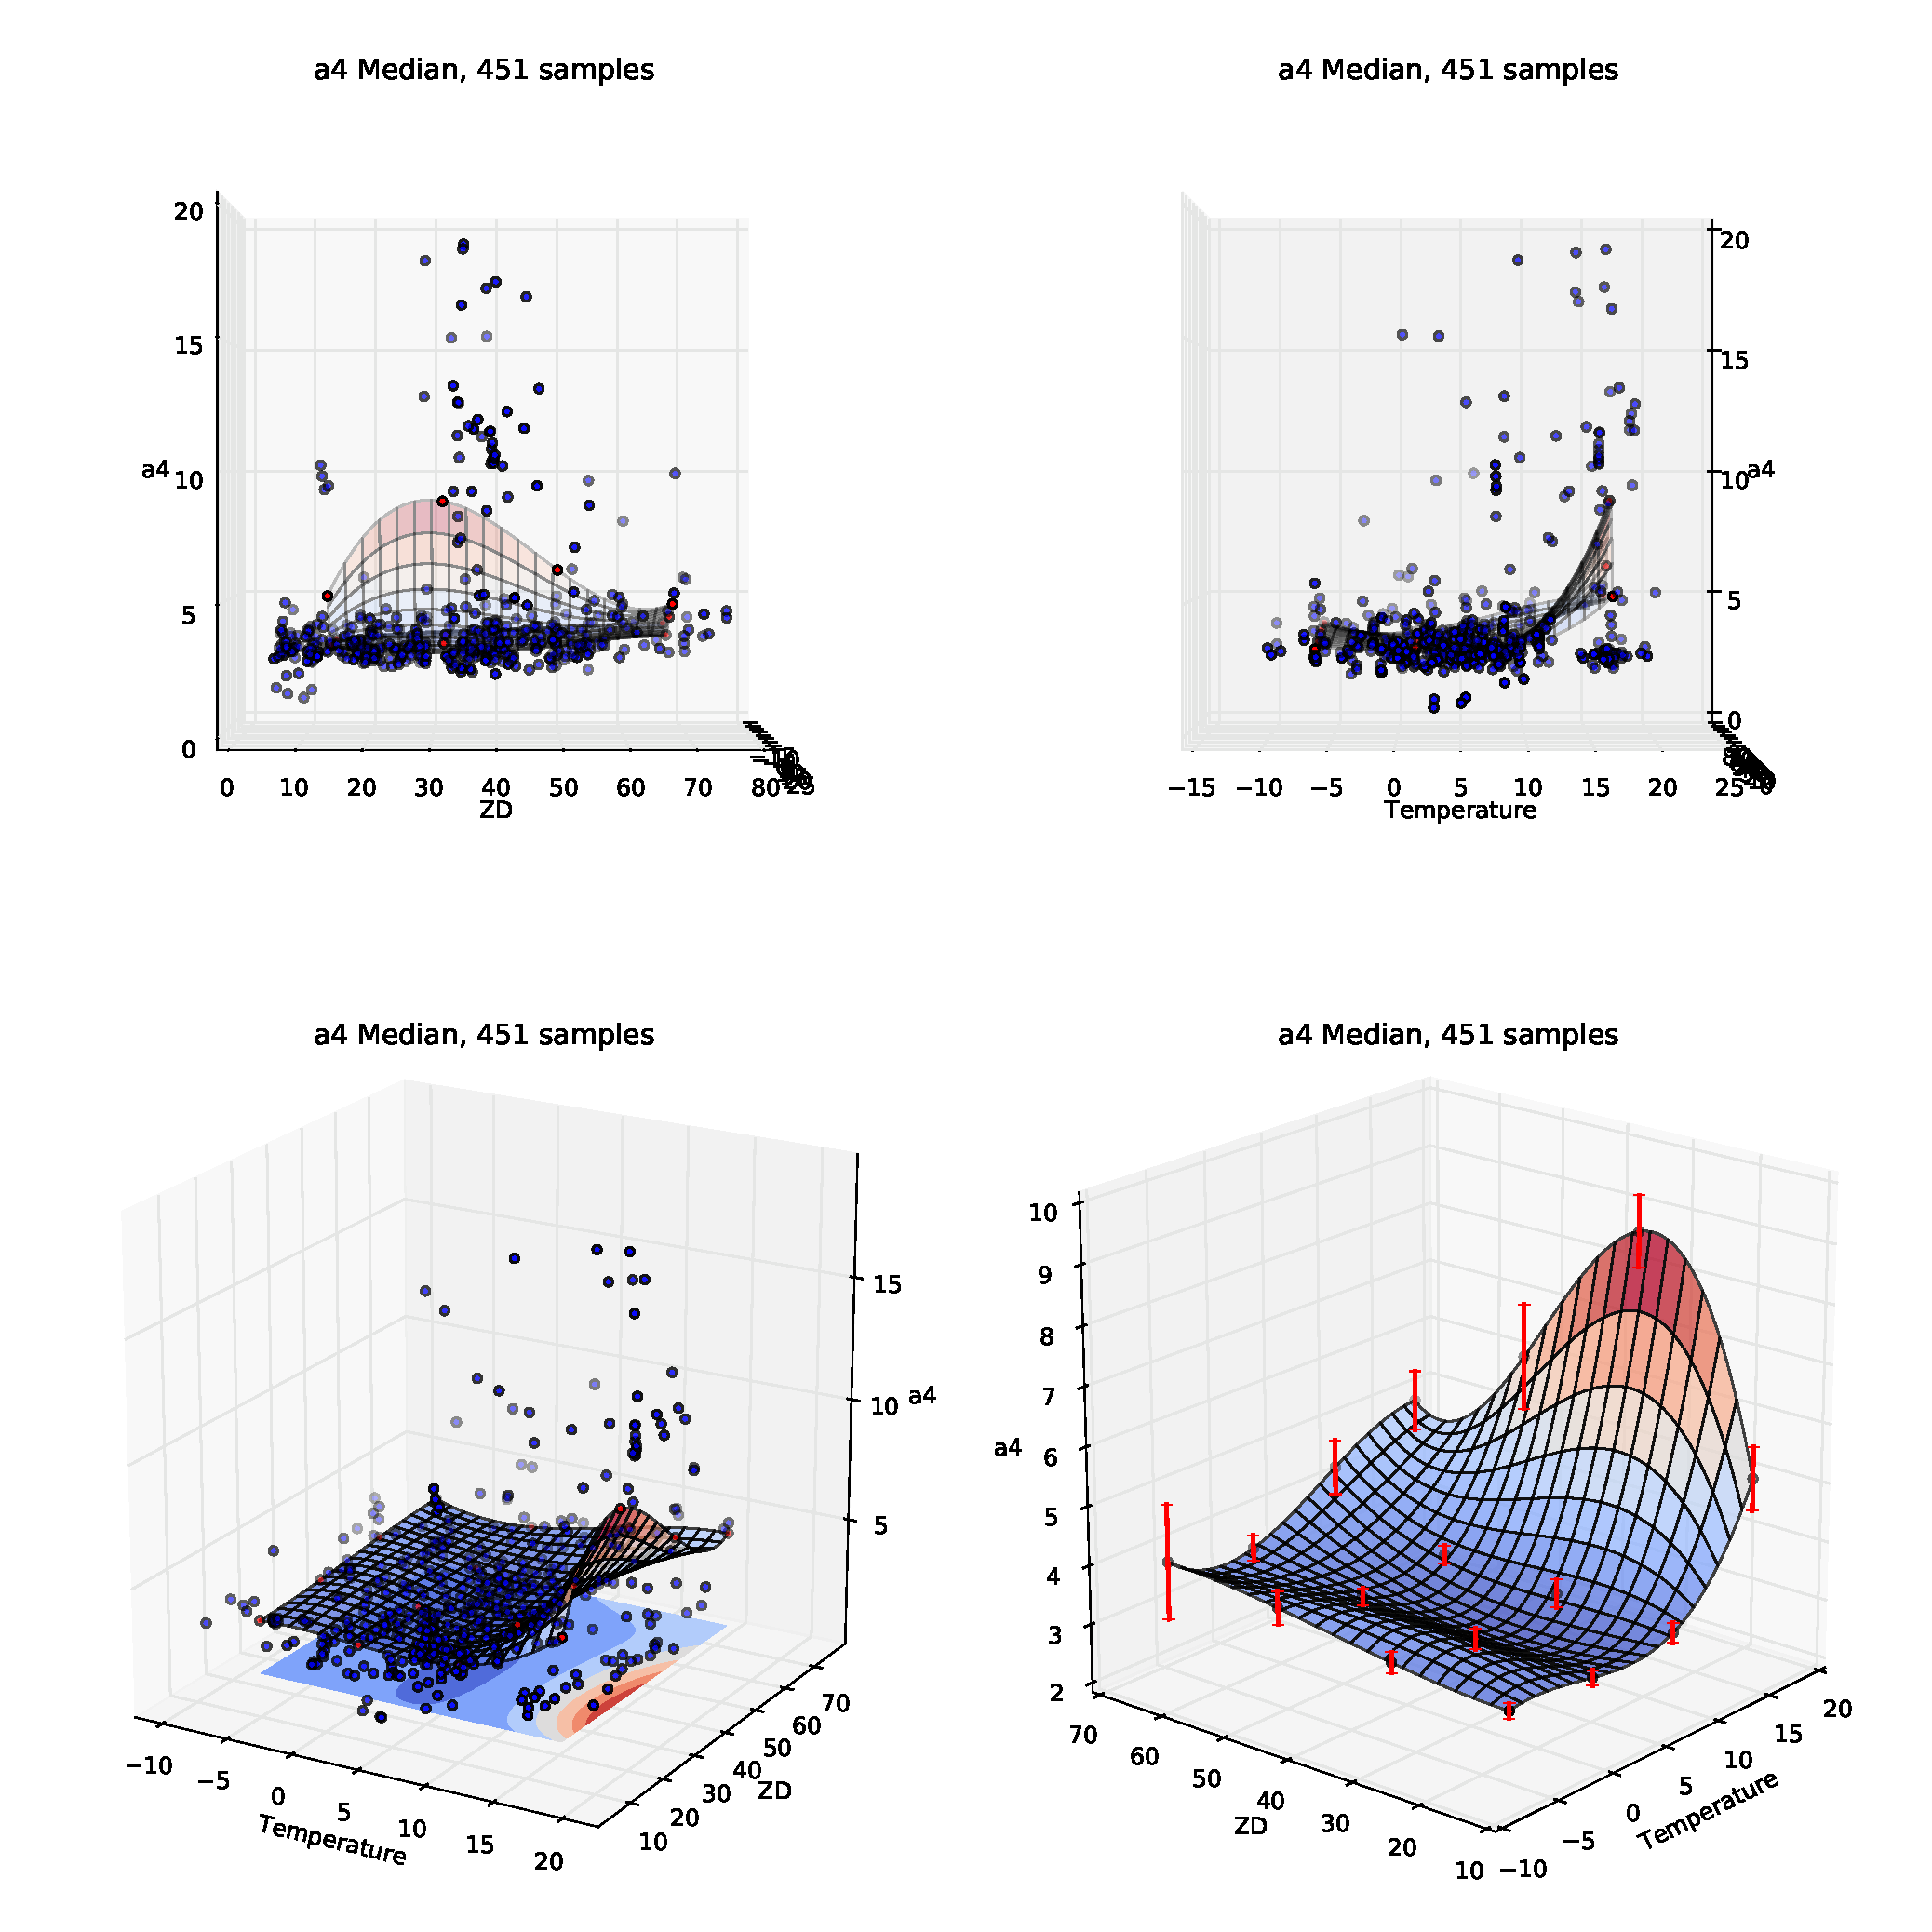
\includegraphics[scale=.48]{psf_surf/a4_med.pdf}
	\caption[Median Streu- und Flächenplot des PSF-Parameters $A_4$]{Median Streu- und Flächenplot des PSF-Parameters $A_4$}
    \label{psf_surf_a4_med}
\end{figure}
\begin{figure}[H]
	\centering
	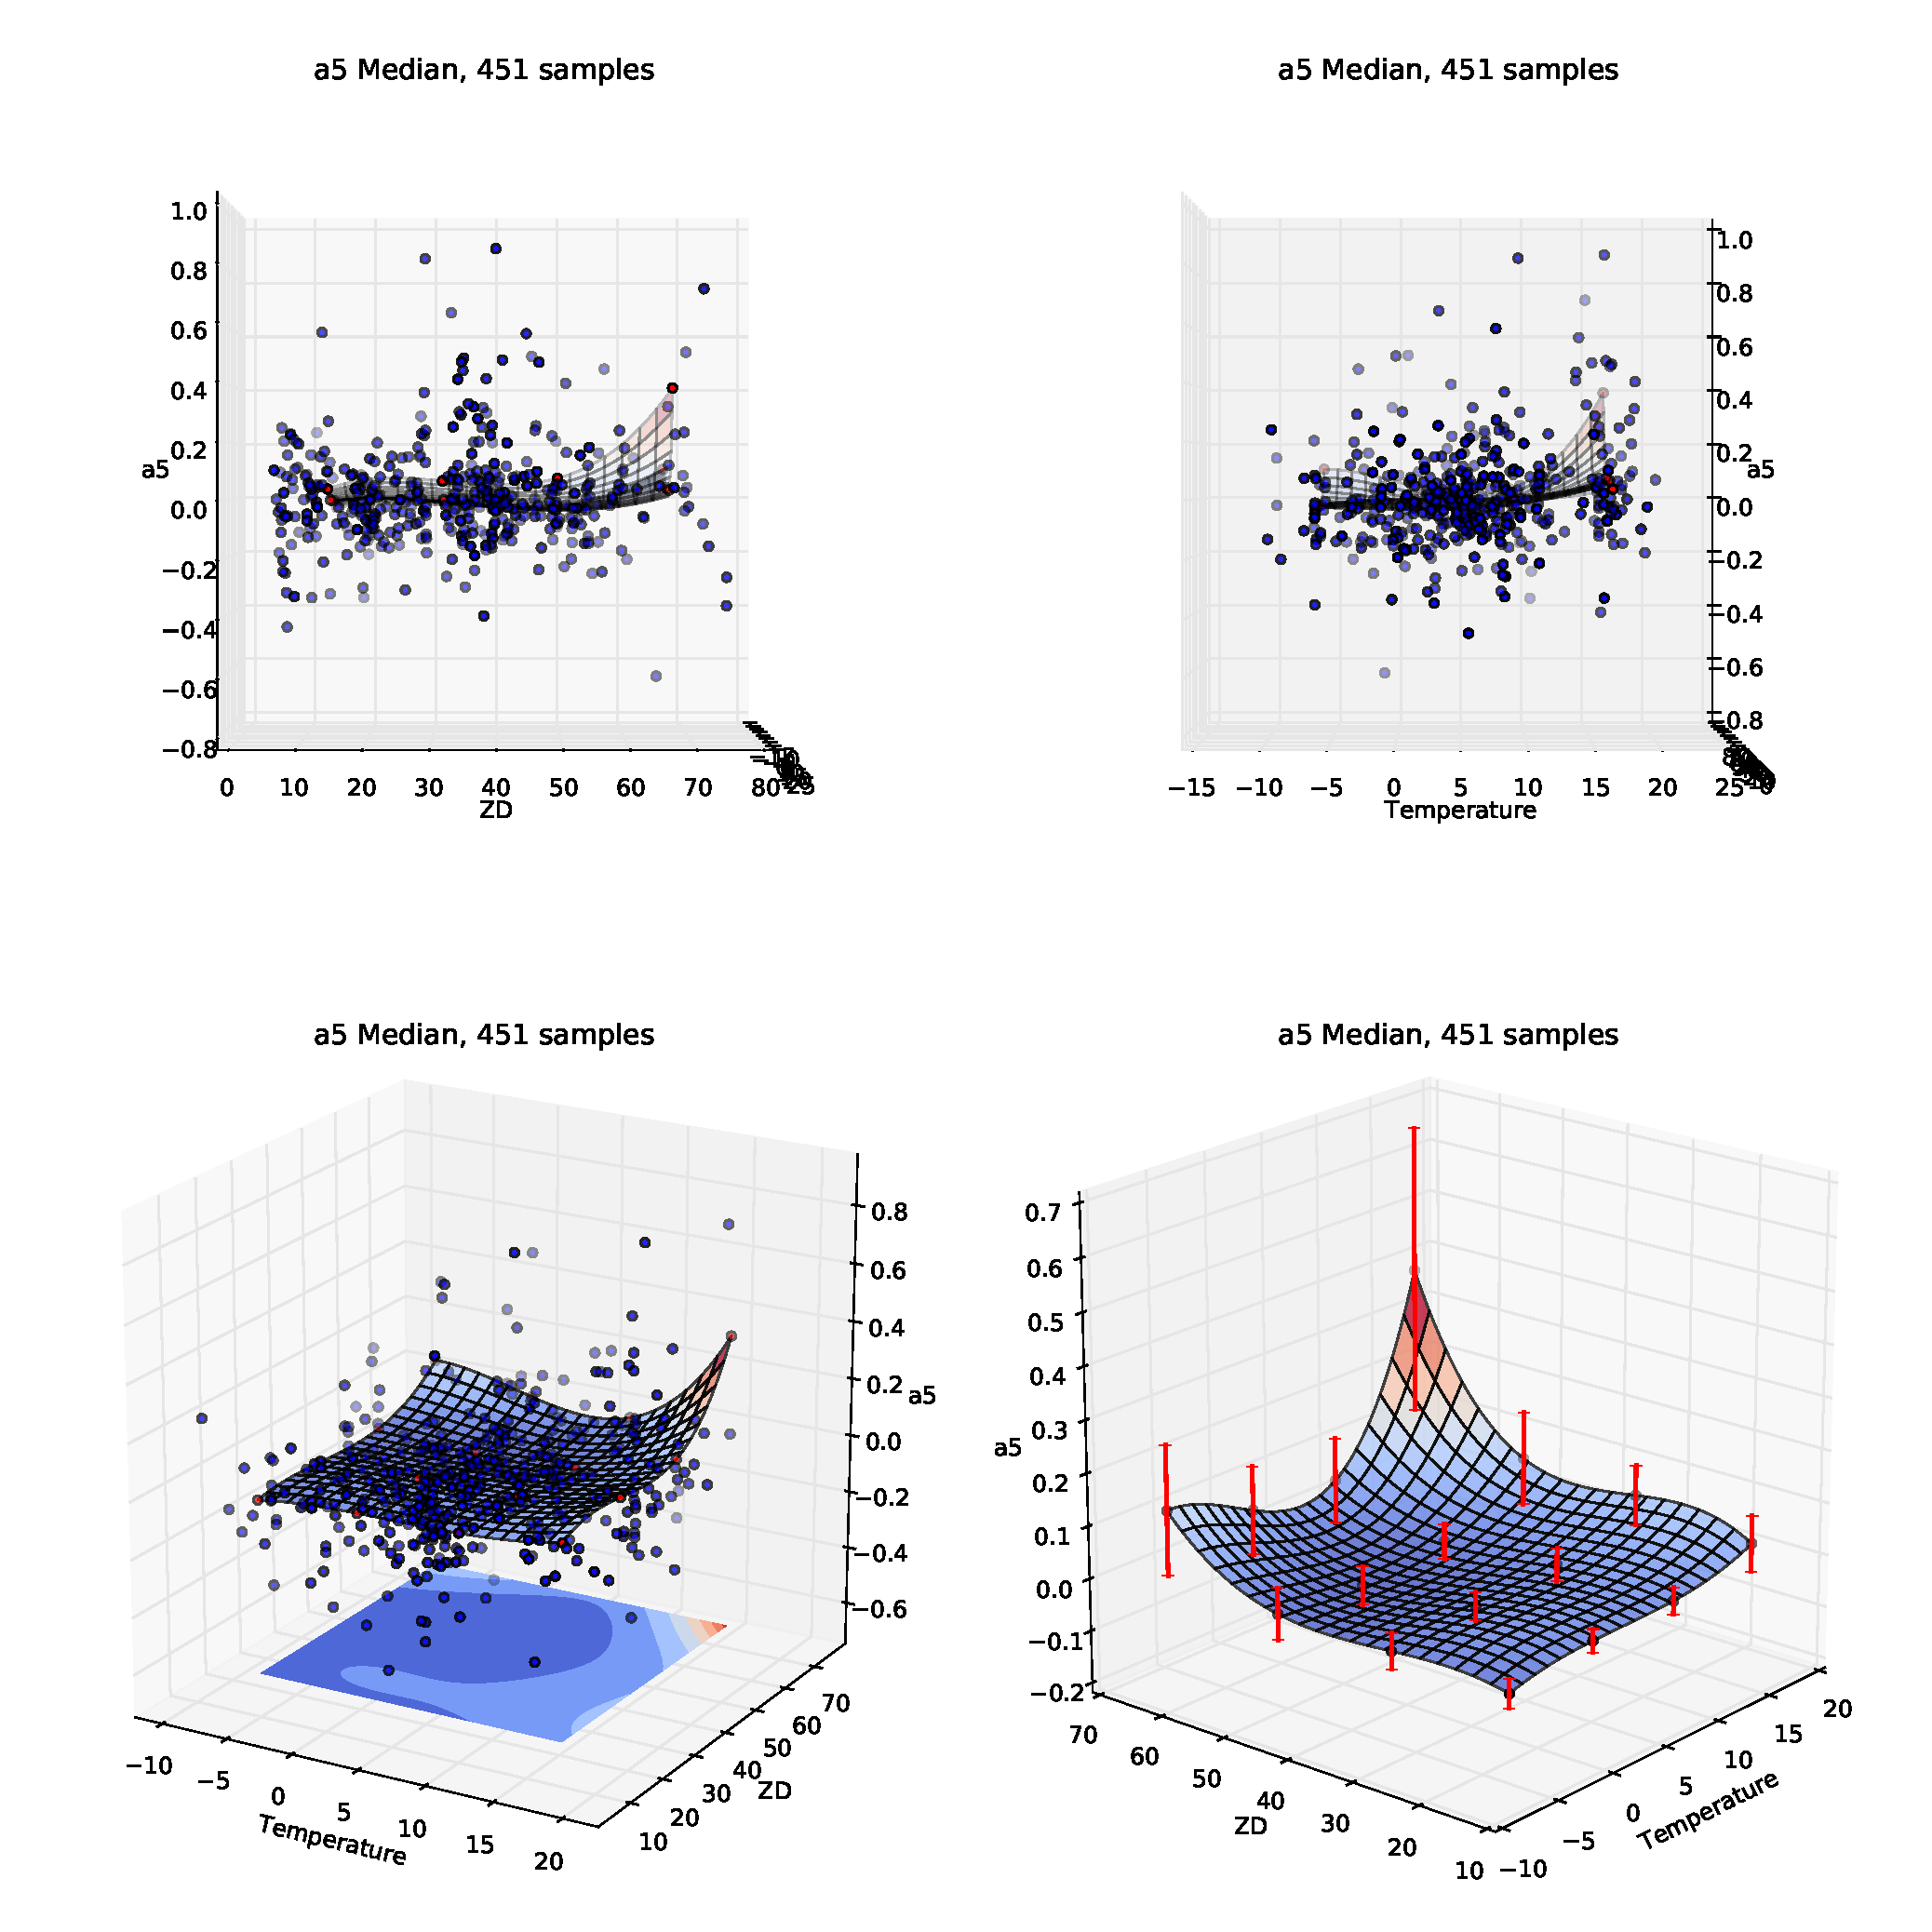
\includegraphics[scale=.48]{psf_surf/a5_med.pdf}
	\caption[Median Streu- und Flächenplot des PSF-Parameters $A_5$]{Median Streu- und Flächenplot des PSF-Parameters $A_5$}
    \label{psf_surf_a5_med}
\end{figure}
\begin{figure}[H]
	\centering
	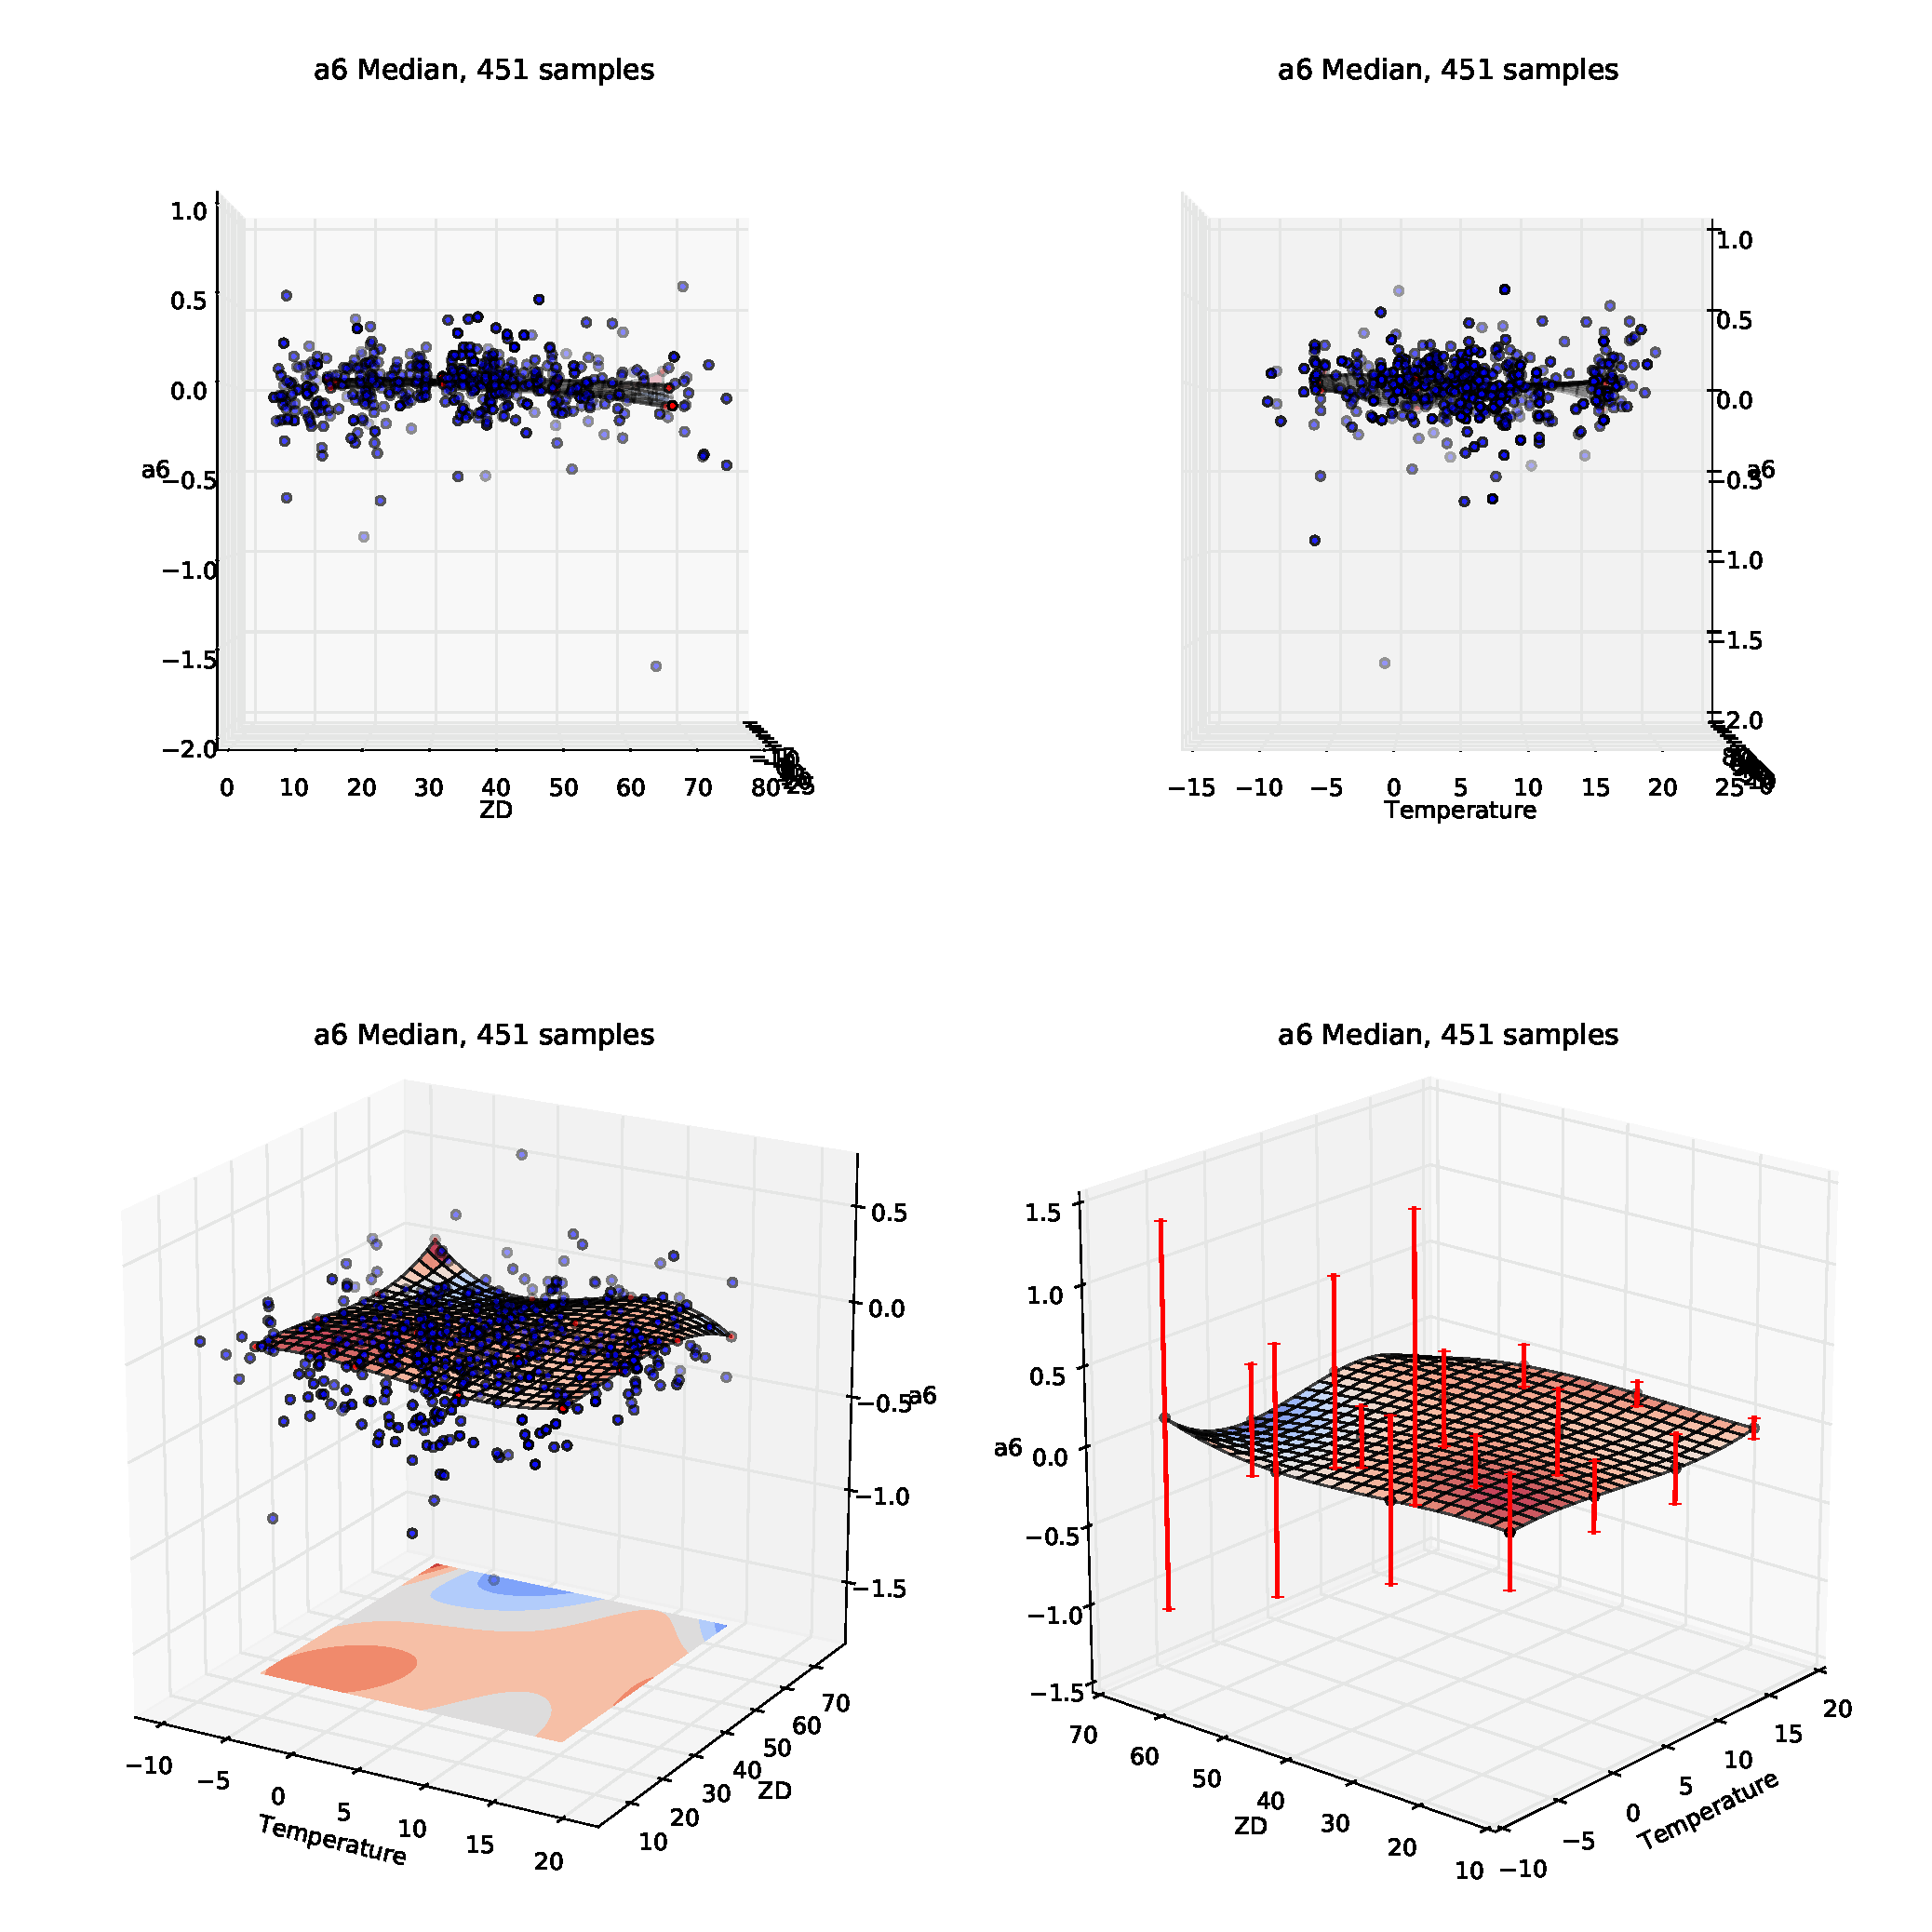
\includegraphics[scale=.48]{psf_surf/a6_med.pdf}
	\caption[Mean Streu- und Flächenplot des PSF-Parameters $A_6$]{Median Streu- und Flächenplot des PSF-Parameters $A_6$}
    \label{psf_surf_a6_med}
\end{figure}

\begin{figure}[H]
	\centering
	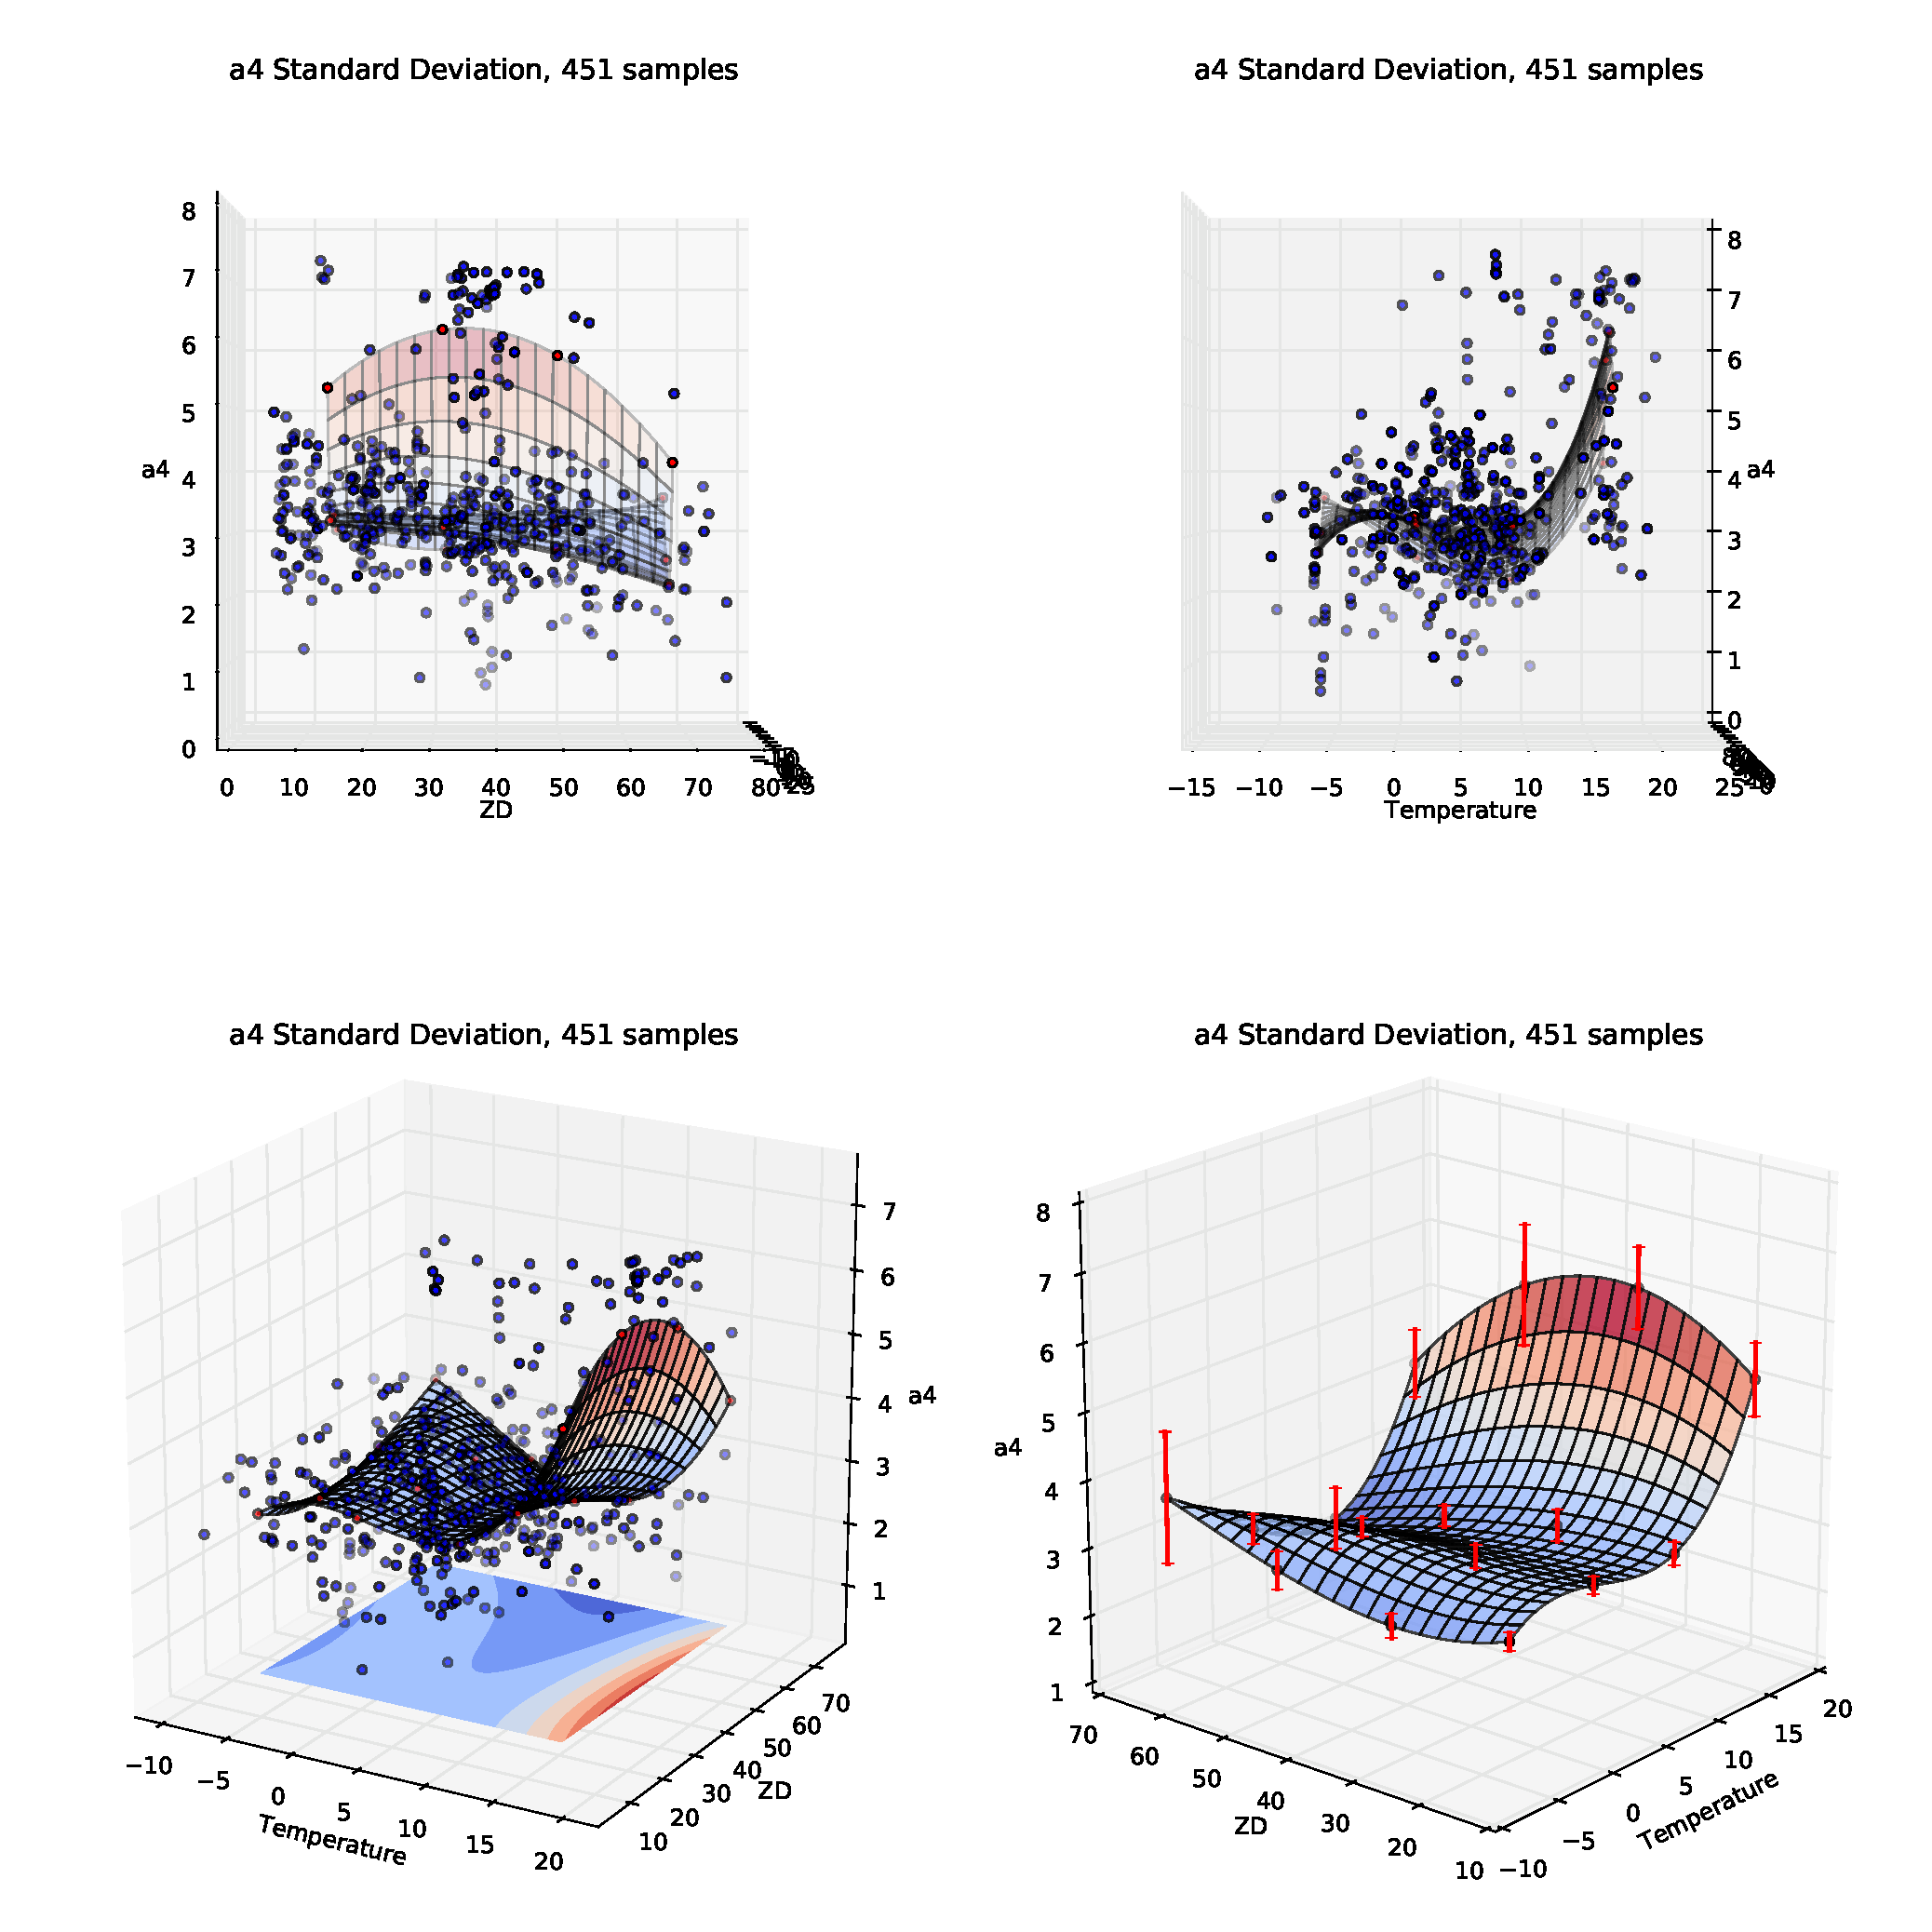
\includegraphics[scale=.48]{psf_surf/a4_std.pdf}
	\caption[Standardabweichung Streu- und Flächenplot des PSF-Parameters $A_4$]{Standardabweichung Streu- und Flächenplot des PSF-Parameters $A_4$}
    \label{psf_surf_a4_std}
\end{figure}
\begin{figure}[H]
	\centering
	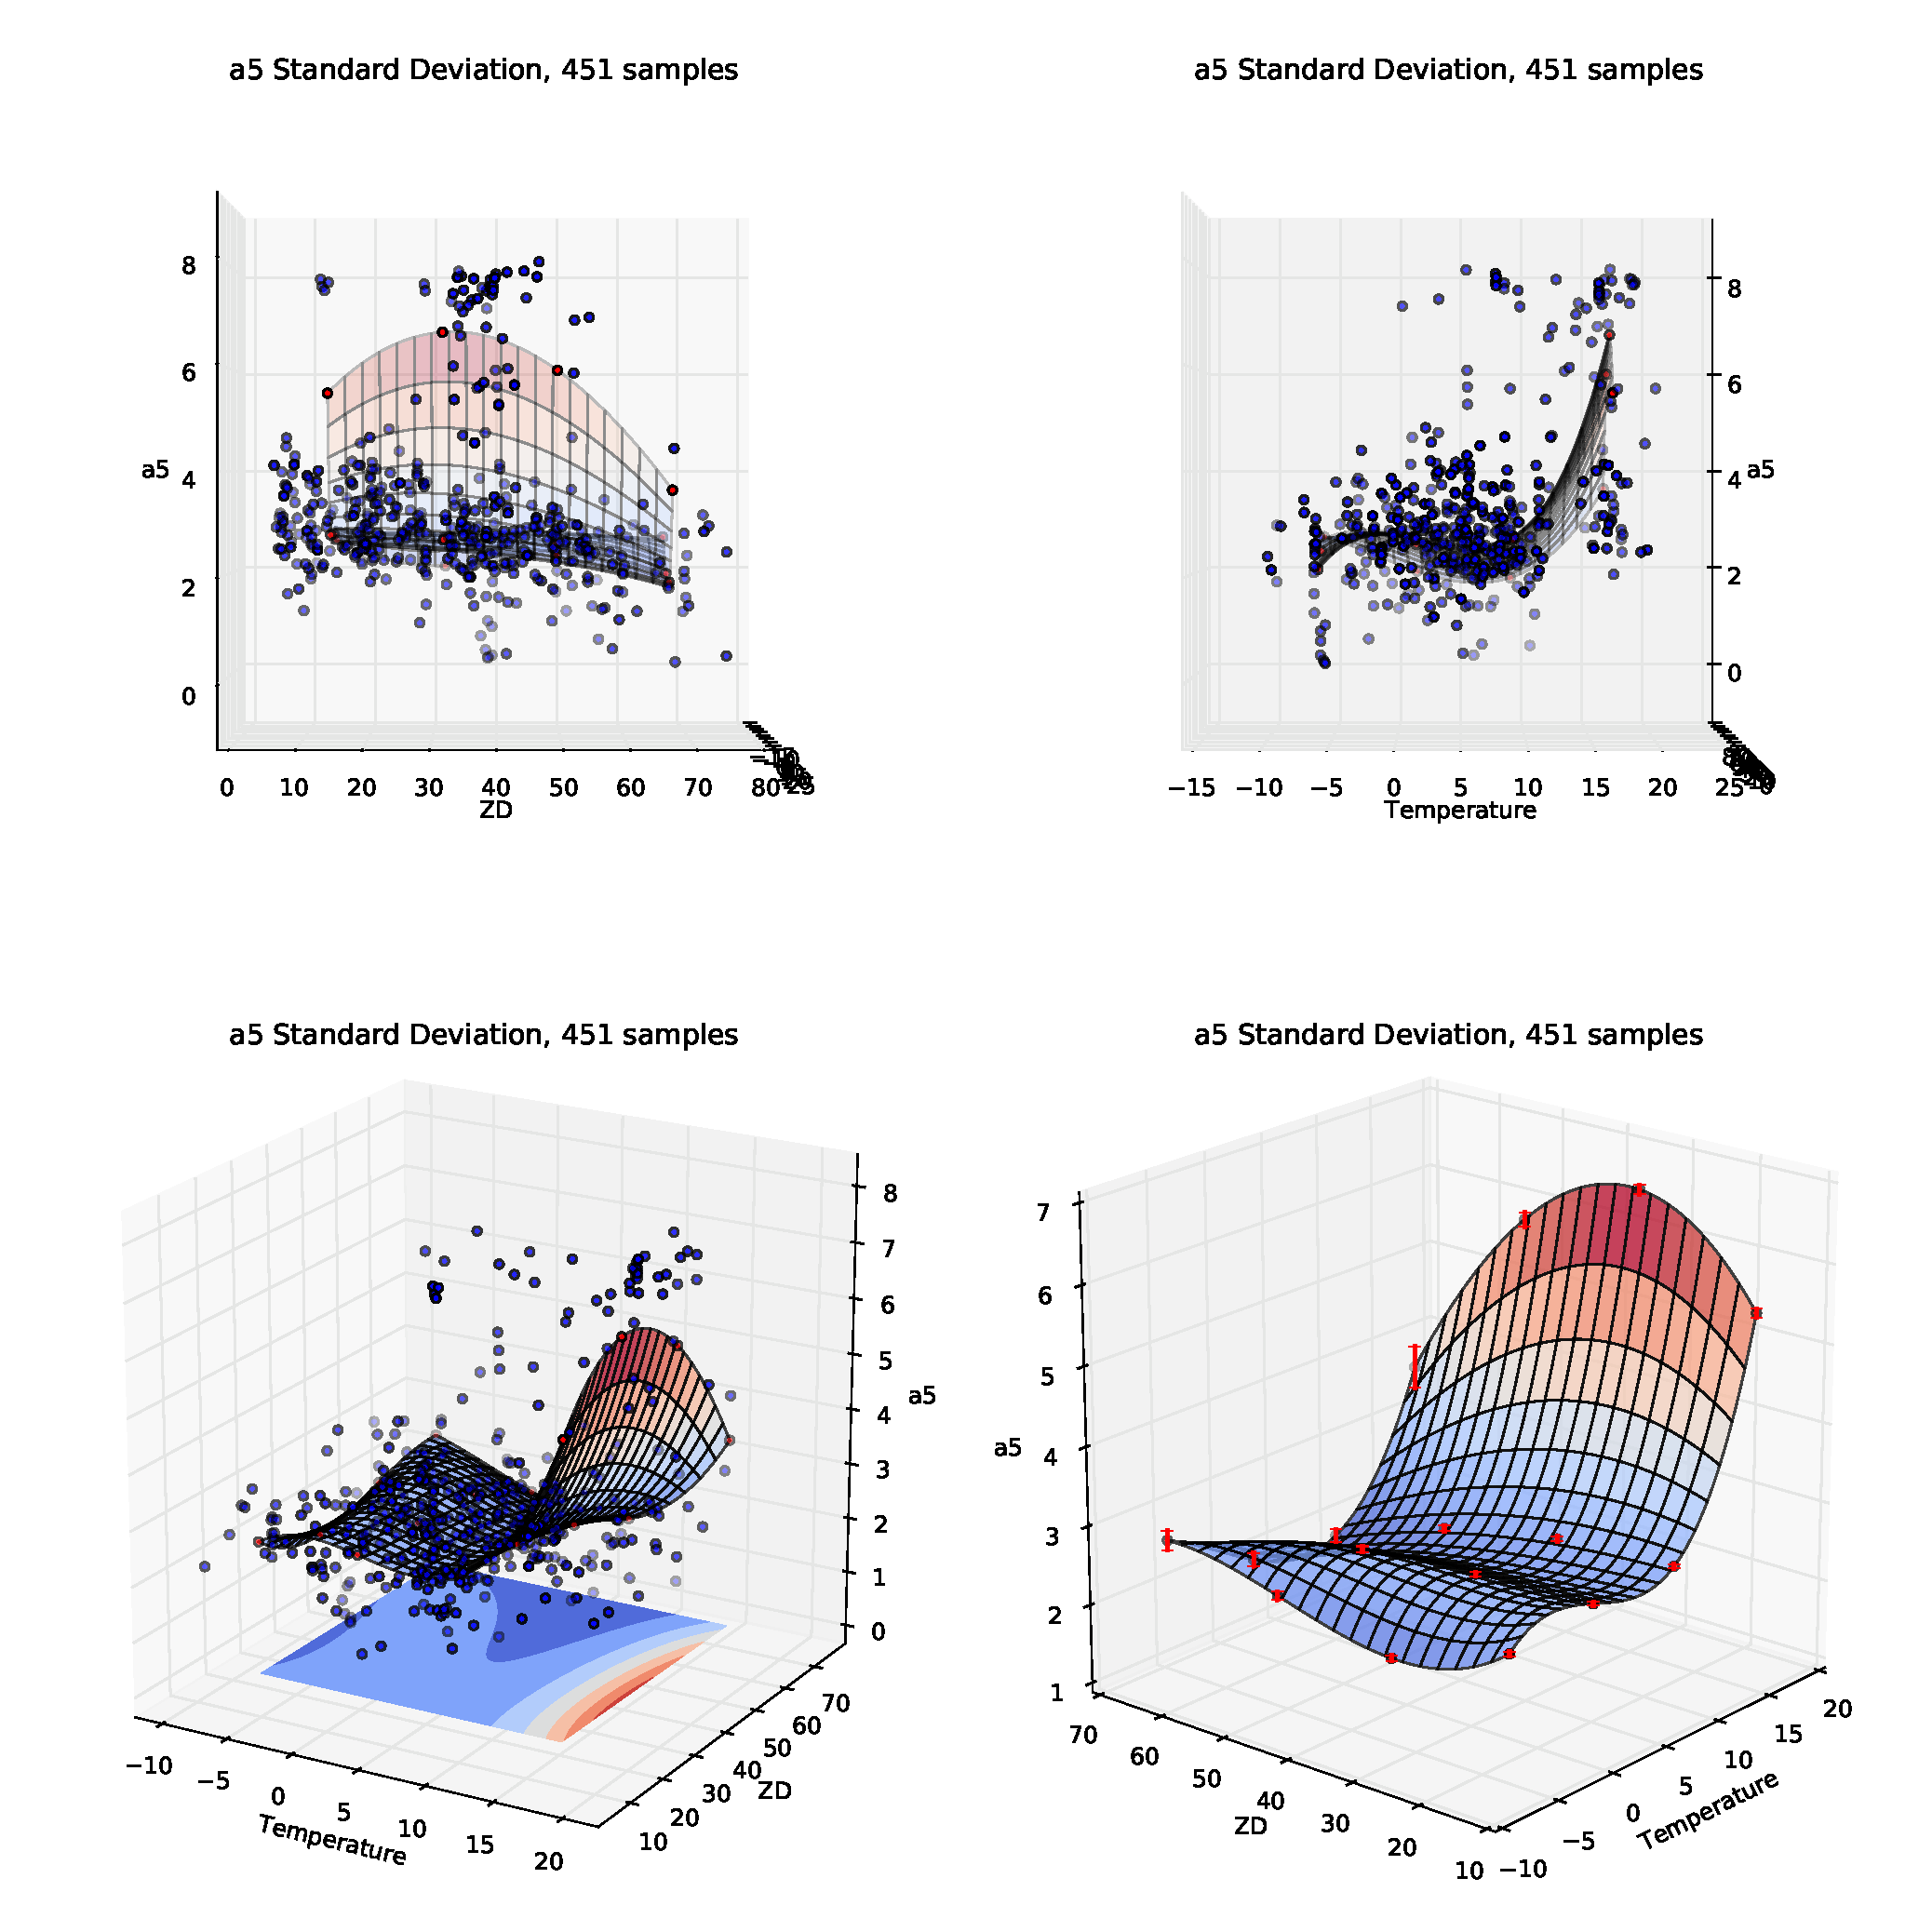
\includegraphics[scale=.48]{psf_surf/a5_std.pdf}
	\caption[Standardabweichung Streu- und Flächenplot des PSF-Parameters $A_5$]{Standardabweichung Streu- und Flächenplot des PSF-Parameters $A_5$}
    \label{psf_surf_a5_std}
\end{figure}
\begin{figure}[H]
	\centering
	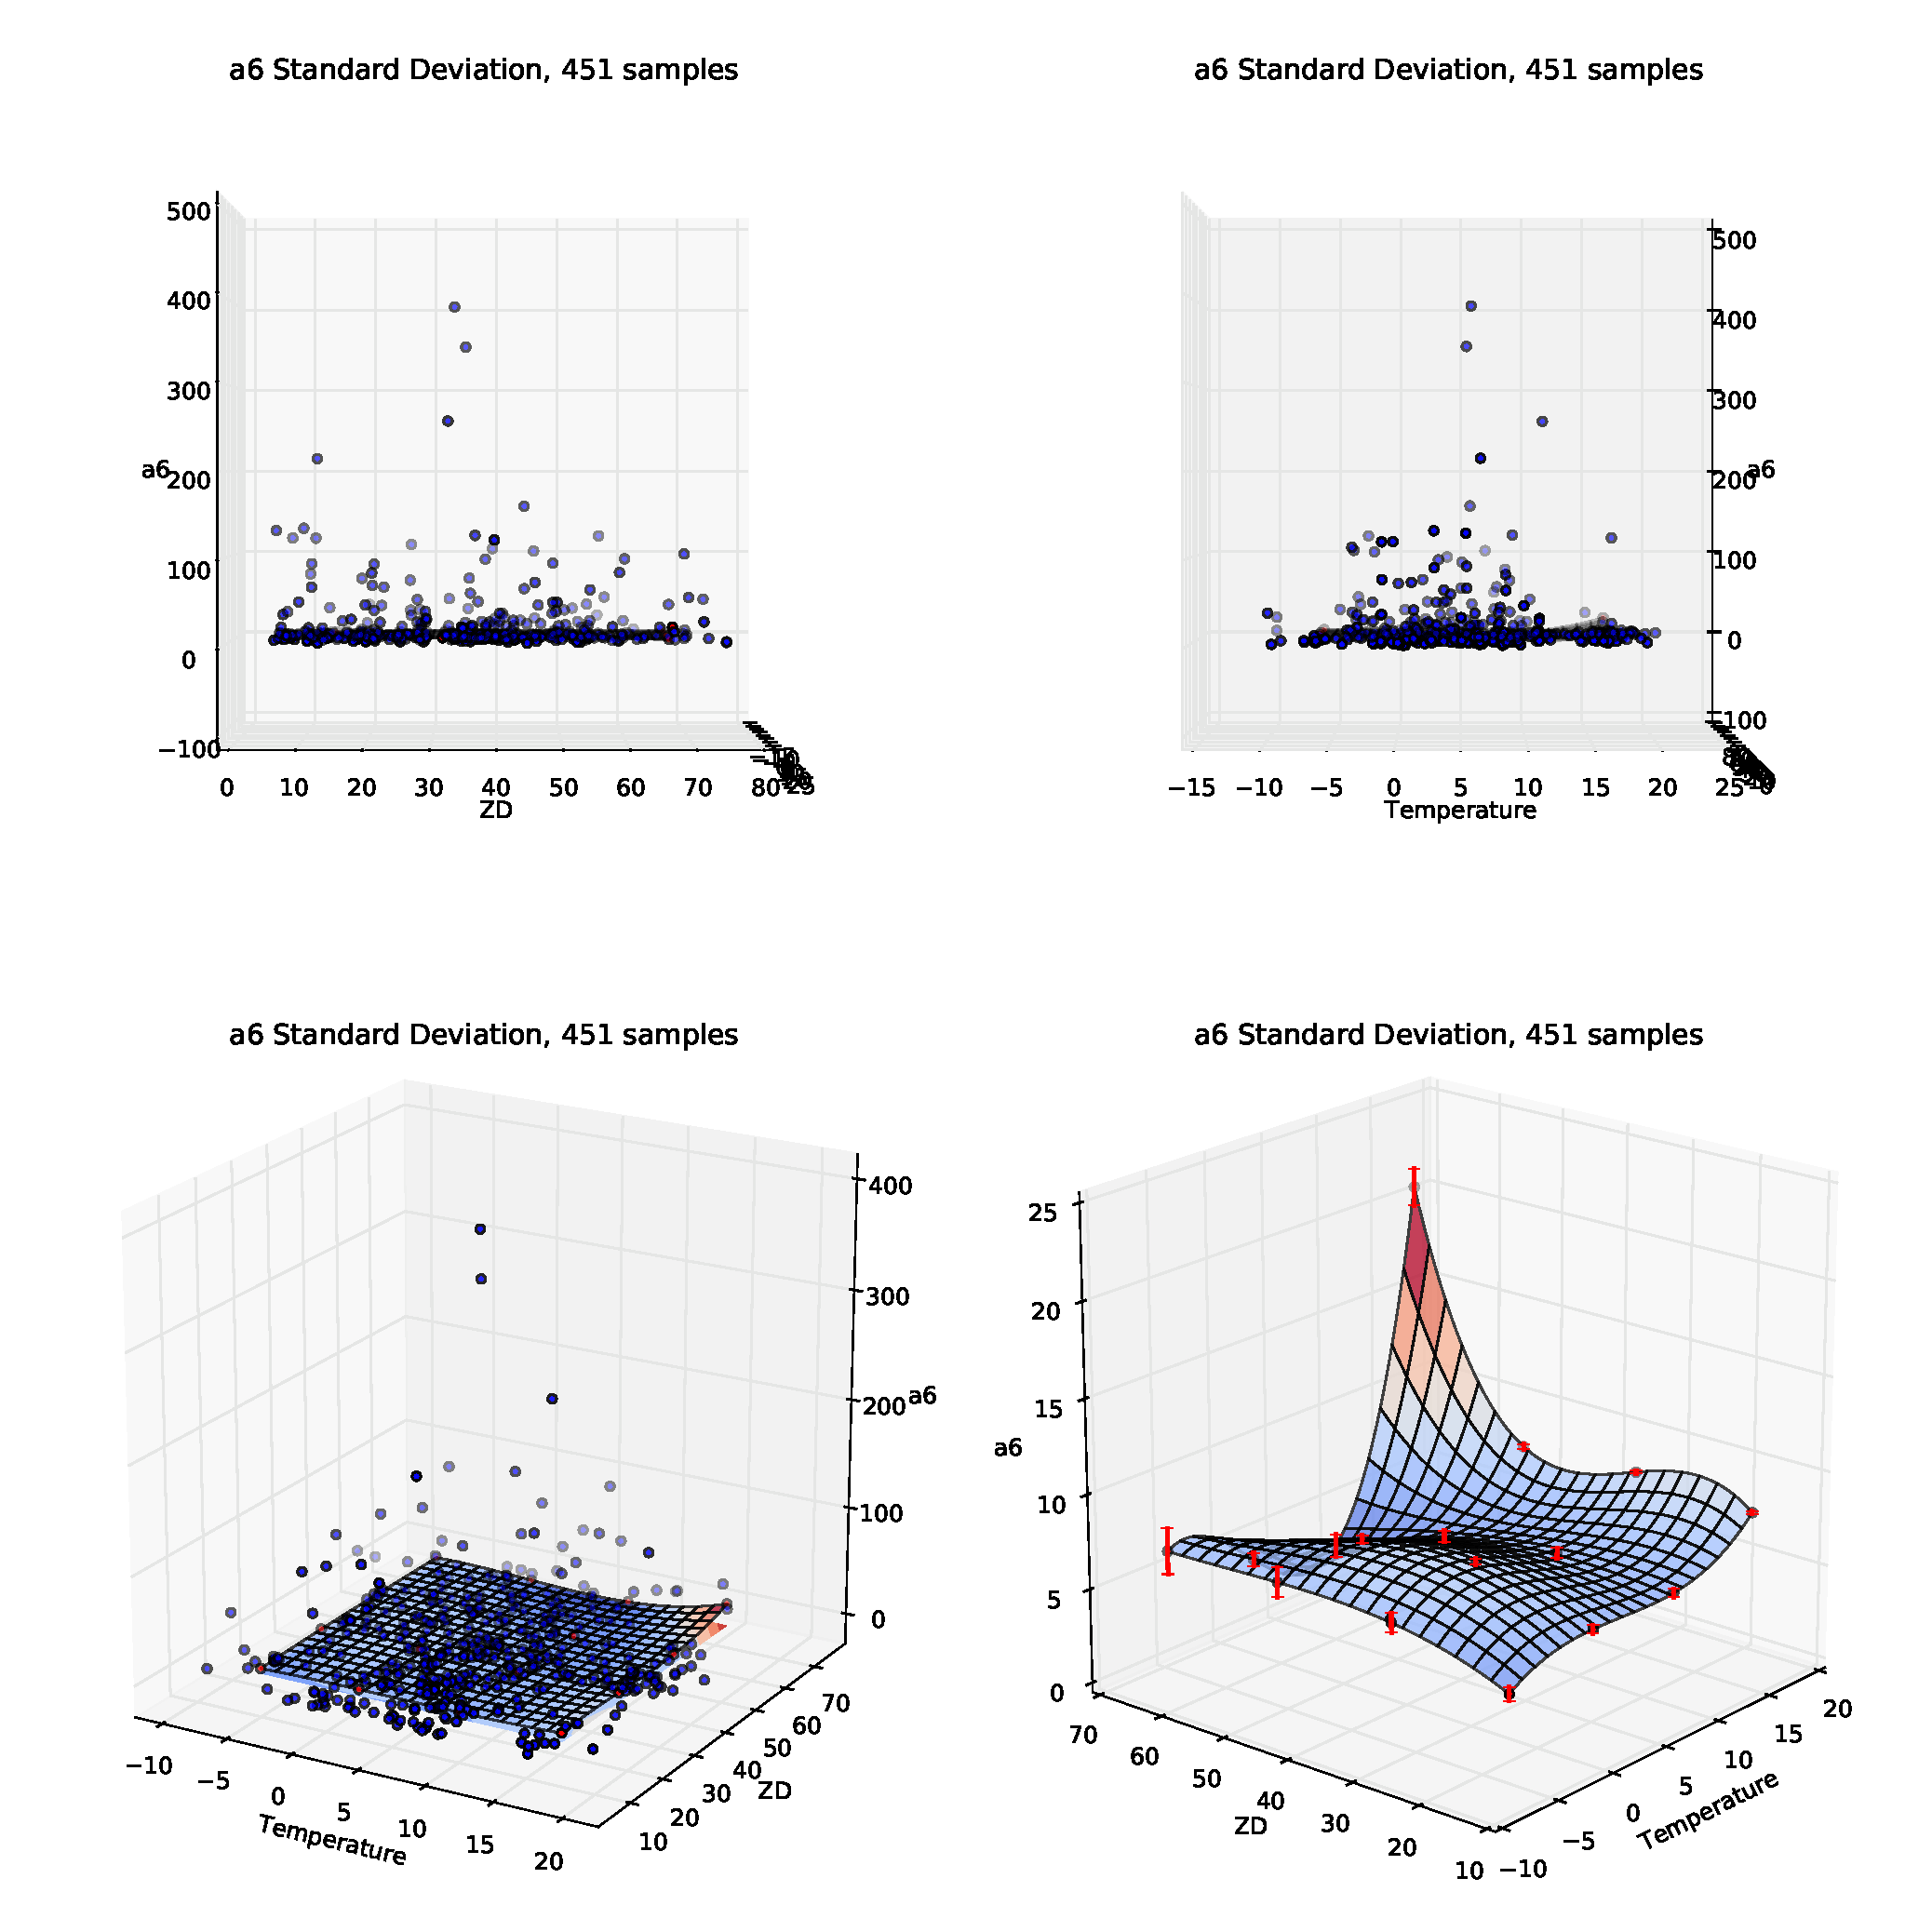
\includegraphics[scale=.48]{psf_surf/a6_std.pdf}
	\caption[Standardabweichung Streu- und Flächenplot des PSF-Parameters $A_6$]{Standardabweichung Streu- und Flächenplot des PSF-Parameters $A_6$}
    \label{psf_surf_a6_std}
\end{figure}

\begin{figure}[H]
	\centering
	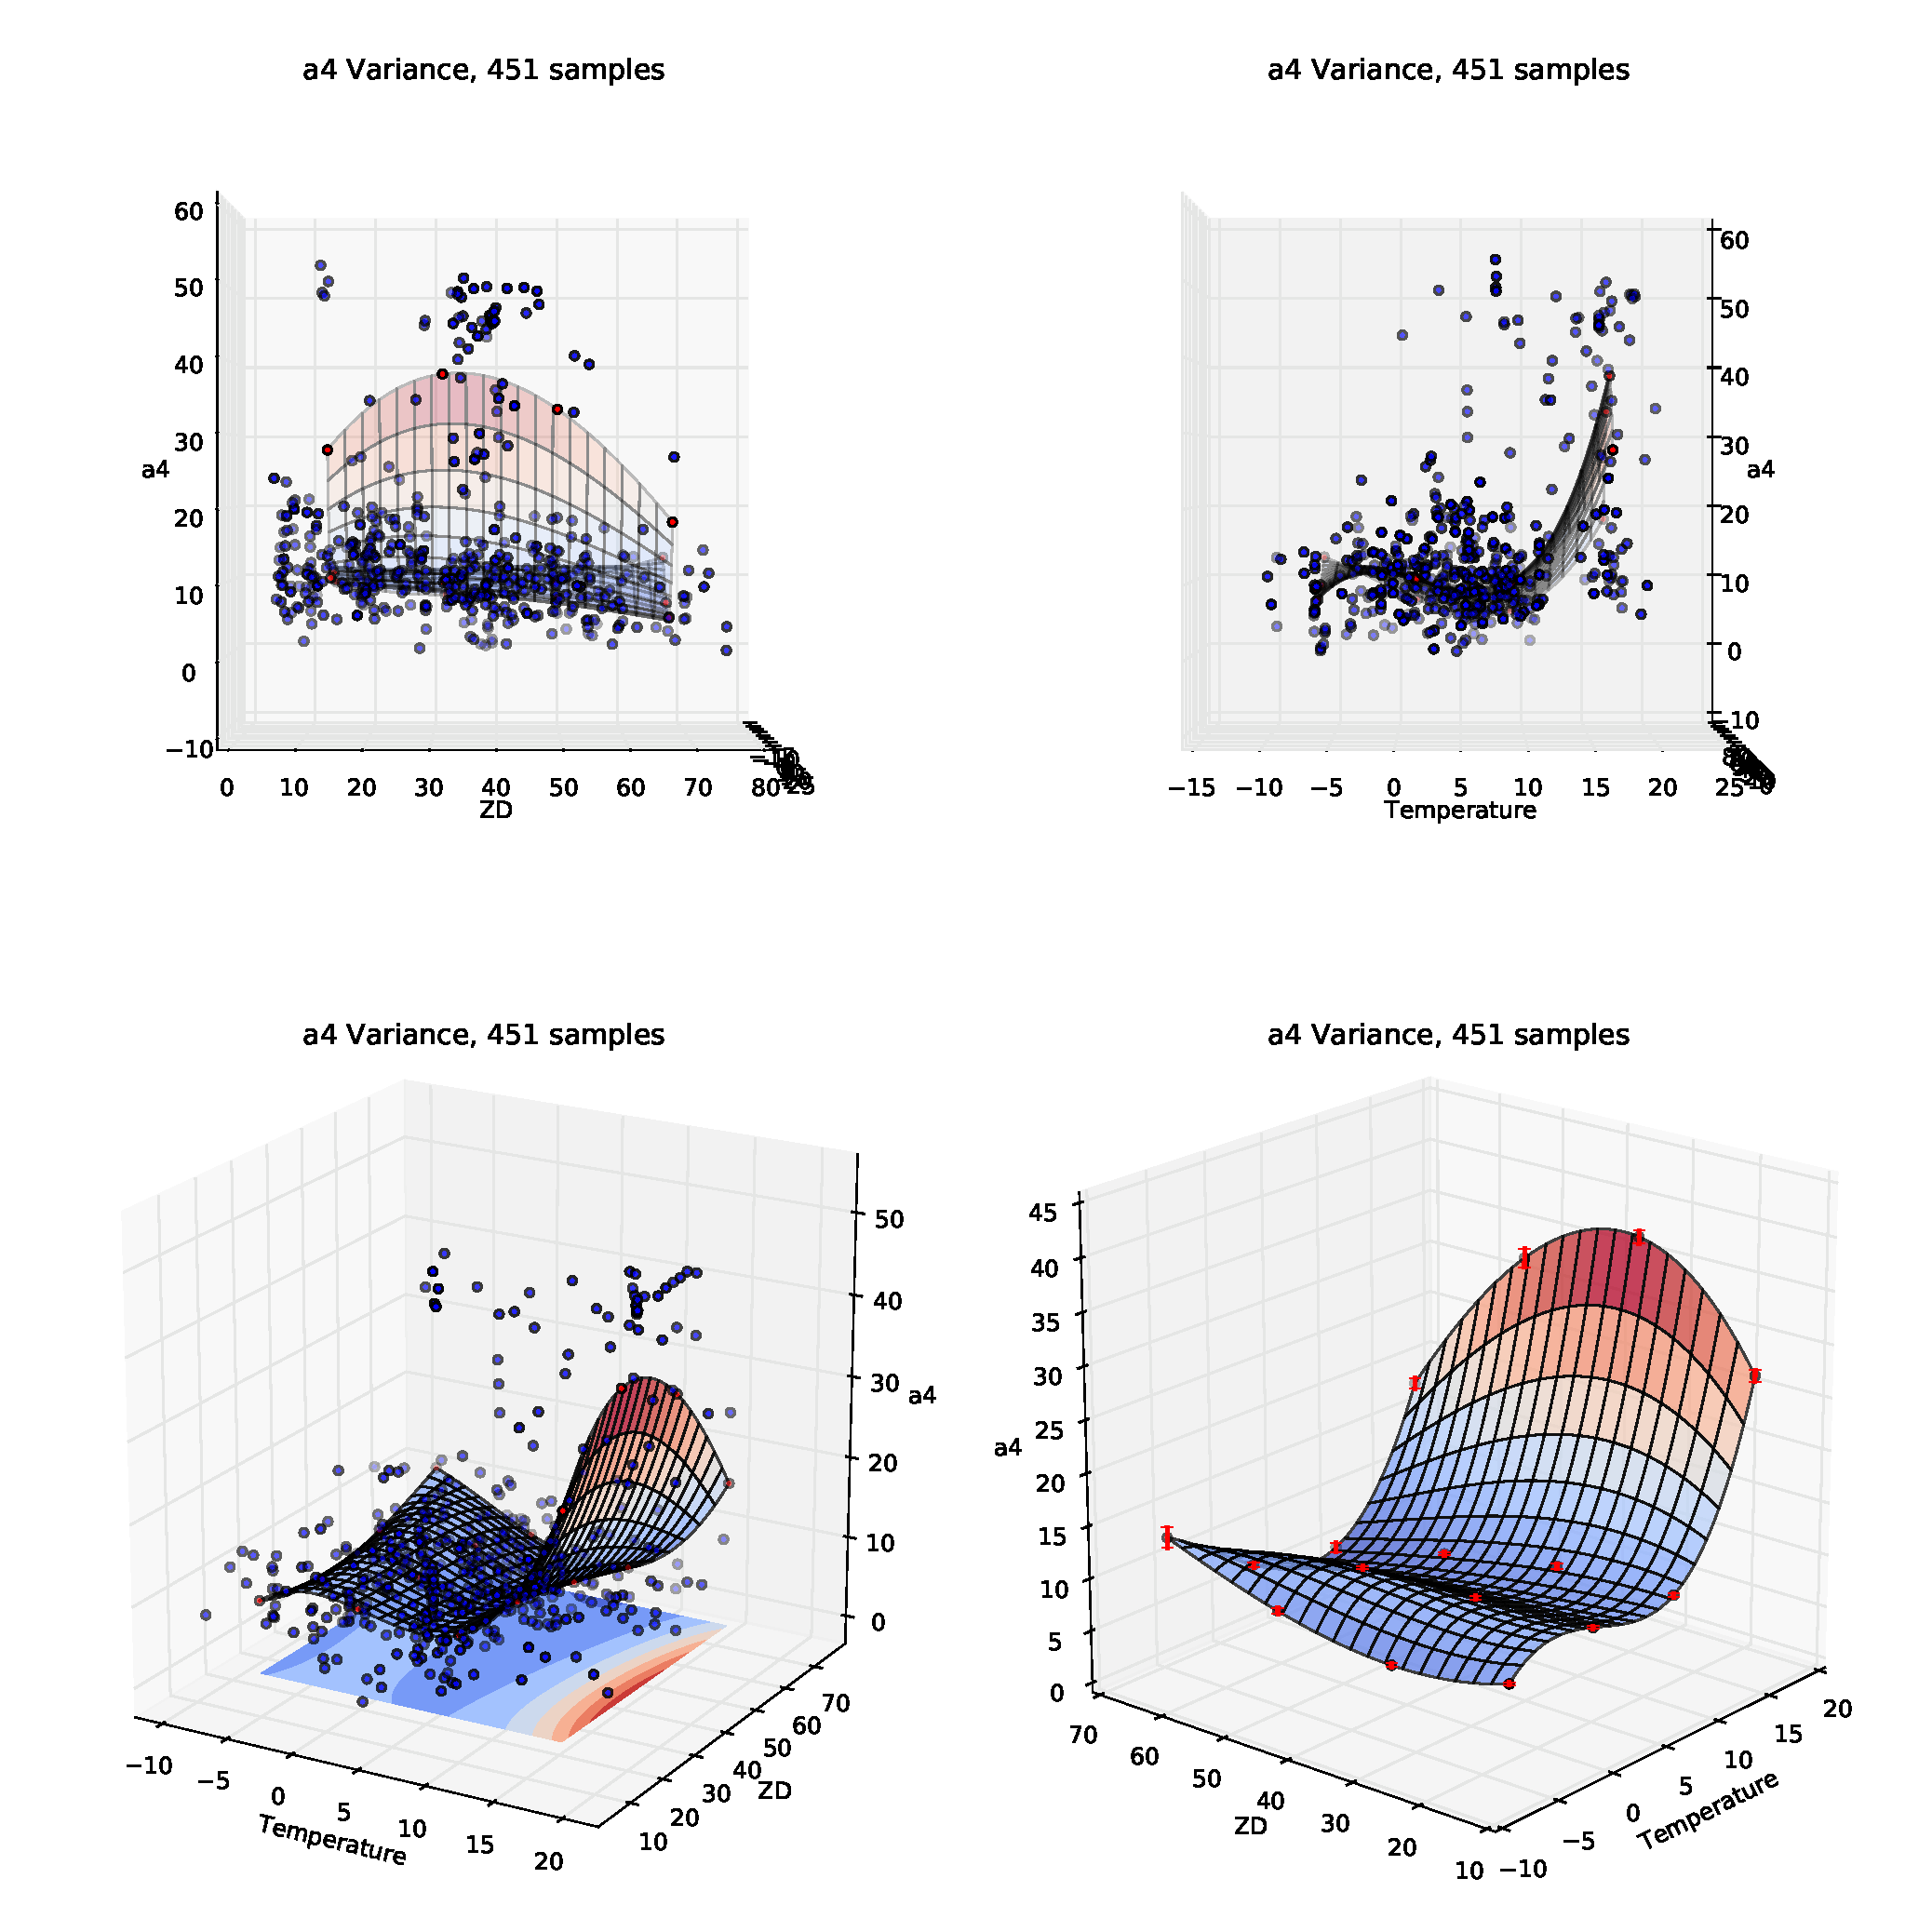
\includegraphics[scale=.48]{psf_surf/a4_var.pdf}
	\caption[Varianz Streu- und Flächenplot des PSF-Parameters $A_4$]{Varianz Streu- und Flächenplot des PSF-Parameters $A_4$}
    \label{psf_surf_a4_var}
\end{figure}
\begin{figure}[H]
	\centering
	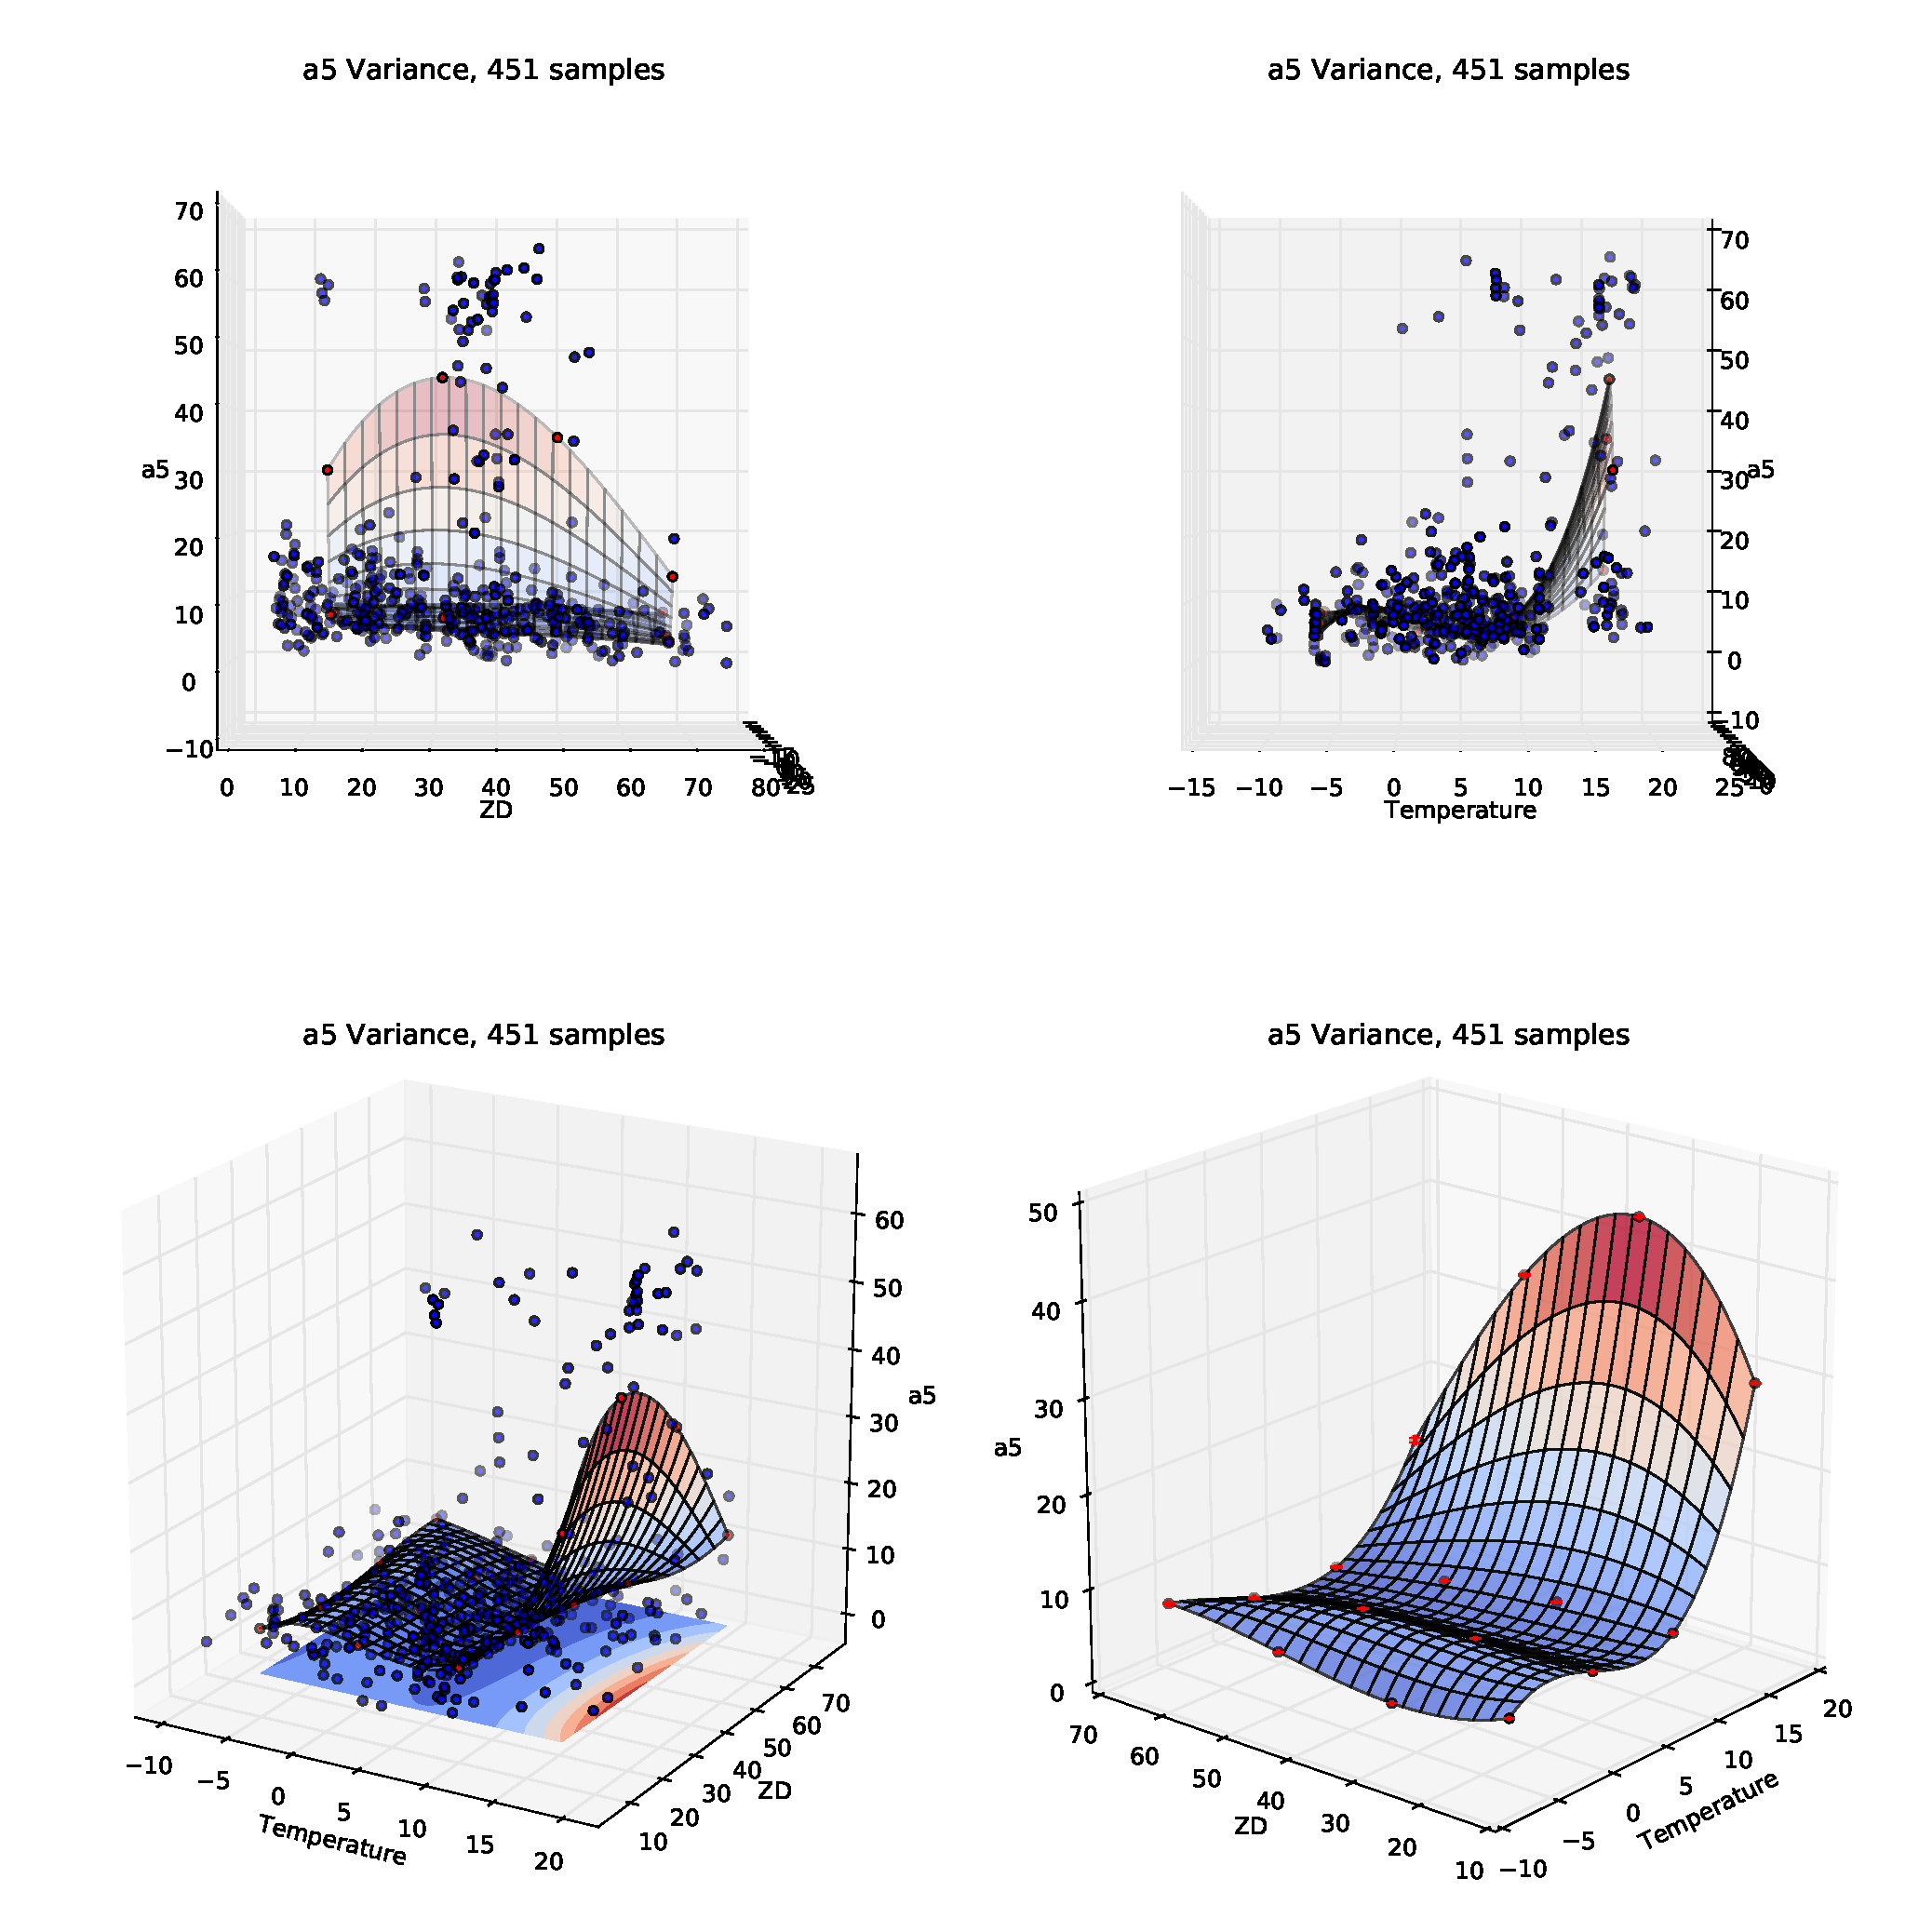
\includegraphics[scale=.48]{psf_surf/a5_var.pdf}
	\caption[Varianz Streu- und Flächenplot des PSF-Parameters $A_5$]{Varianz Streu- und Flächenplot des PSF-Parameters $A_5$}
    \label{psf_surf_a5_var}
\end{figure}
\begin{figure}[H]
	\centering
	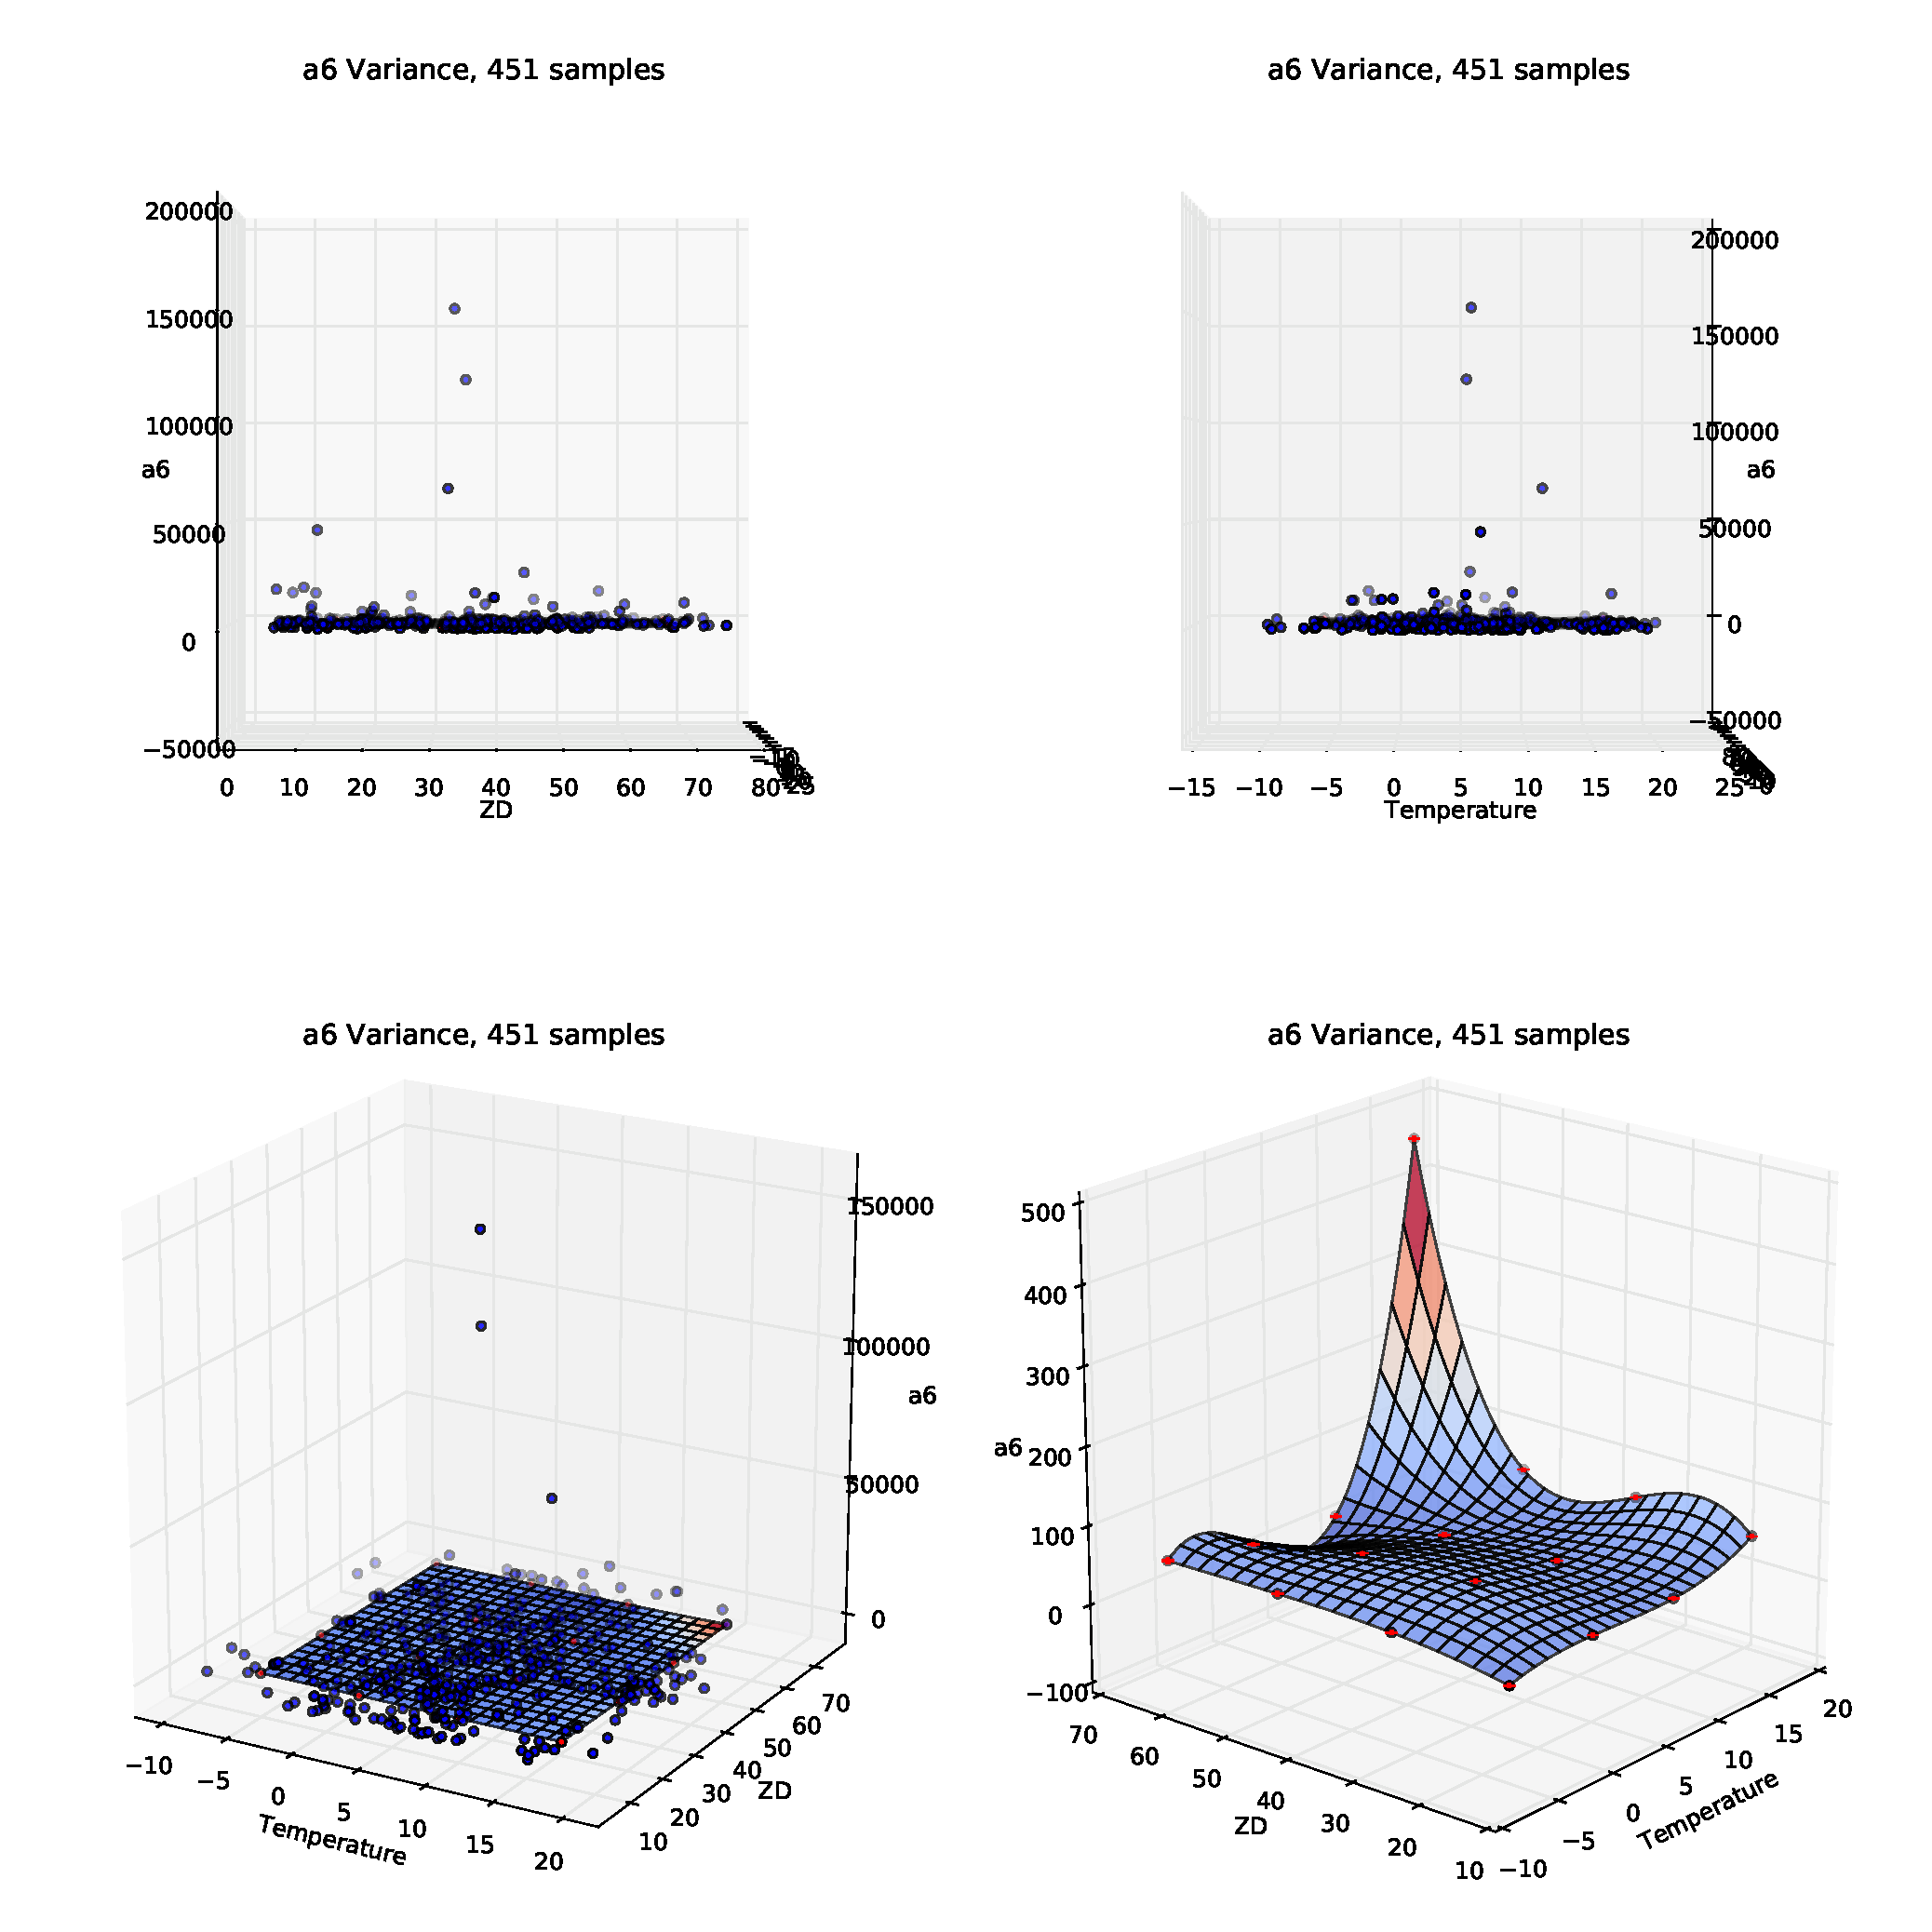
\includegraphics[scale=.48]{psf_surf/a6_var.pdf}
	\caption[Varianz Streu- und Flächenplot des PSF-Parameters $A_6$]{Varianz Streu- und Flächenplot des PSF-Parameters $A_6$}
    \label{psf_surf_a6_var}
\end{figure}

\section{TSI-Verteilungen}
Die TSI-Parameter sind zu zahlreich um alle 124 nicht-statischen diskreten Verteilungsfunktionen an dieser Stelle aufzuzeigen. Stattdessen können sie bei Bedarf online nachgeschlagen oder heruntergeladen werden.
\begin{mdframed}[style=emphasis]
	\centering
	\url{http://homepages.physik.uni-muenchen.de/~Jean.Elsner/focus-series/plots/}
\end{mdframed}
\vfill\,

\section{Sekundärspiegel Temperatur- und Elevationsabhängigkeit}

\begin{figure}[H]
	\centering
	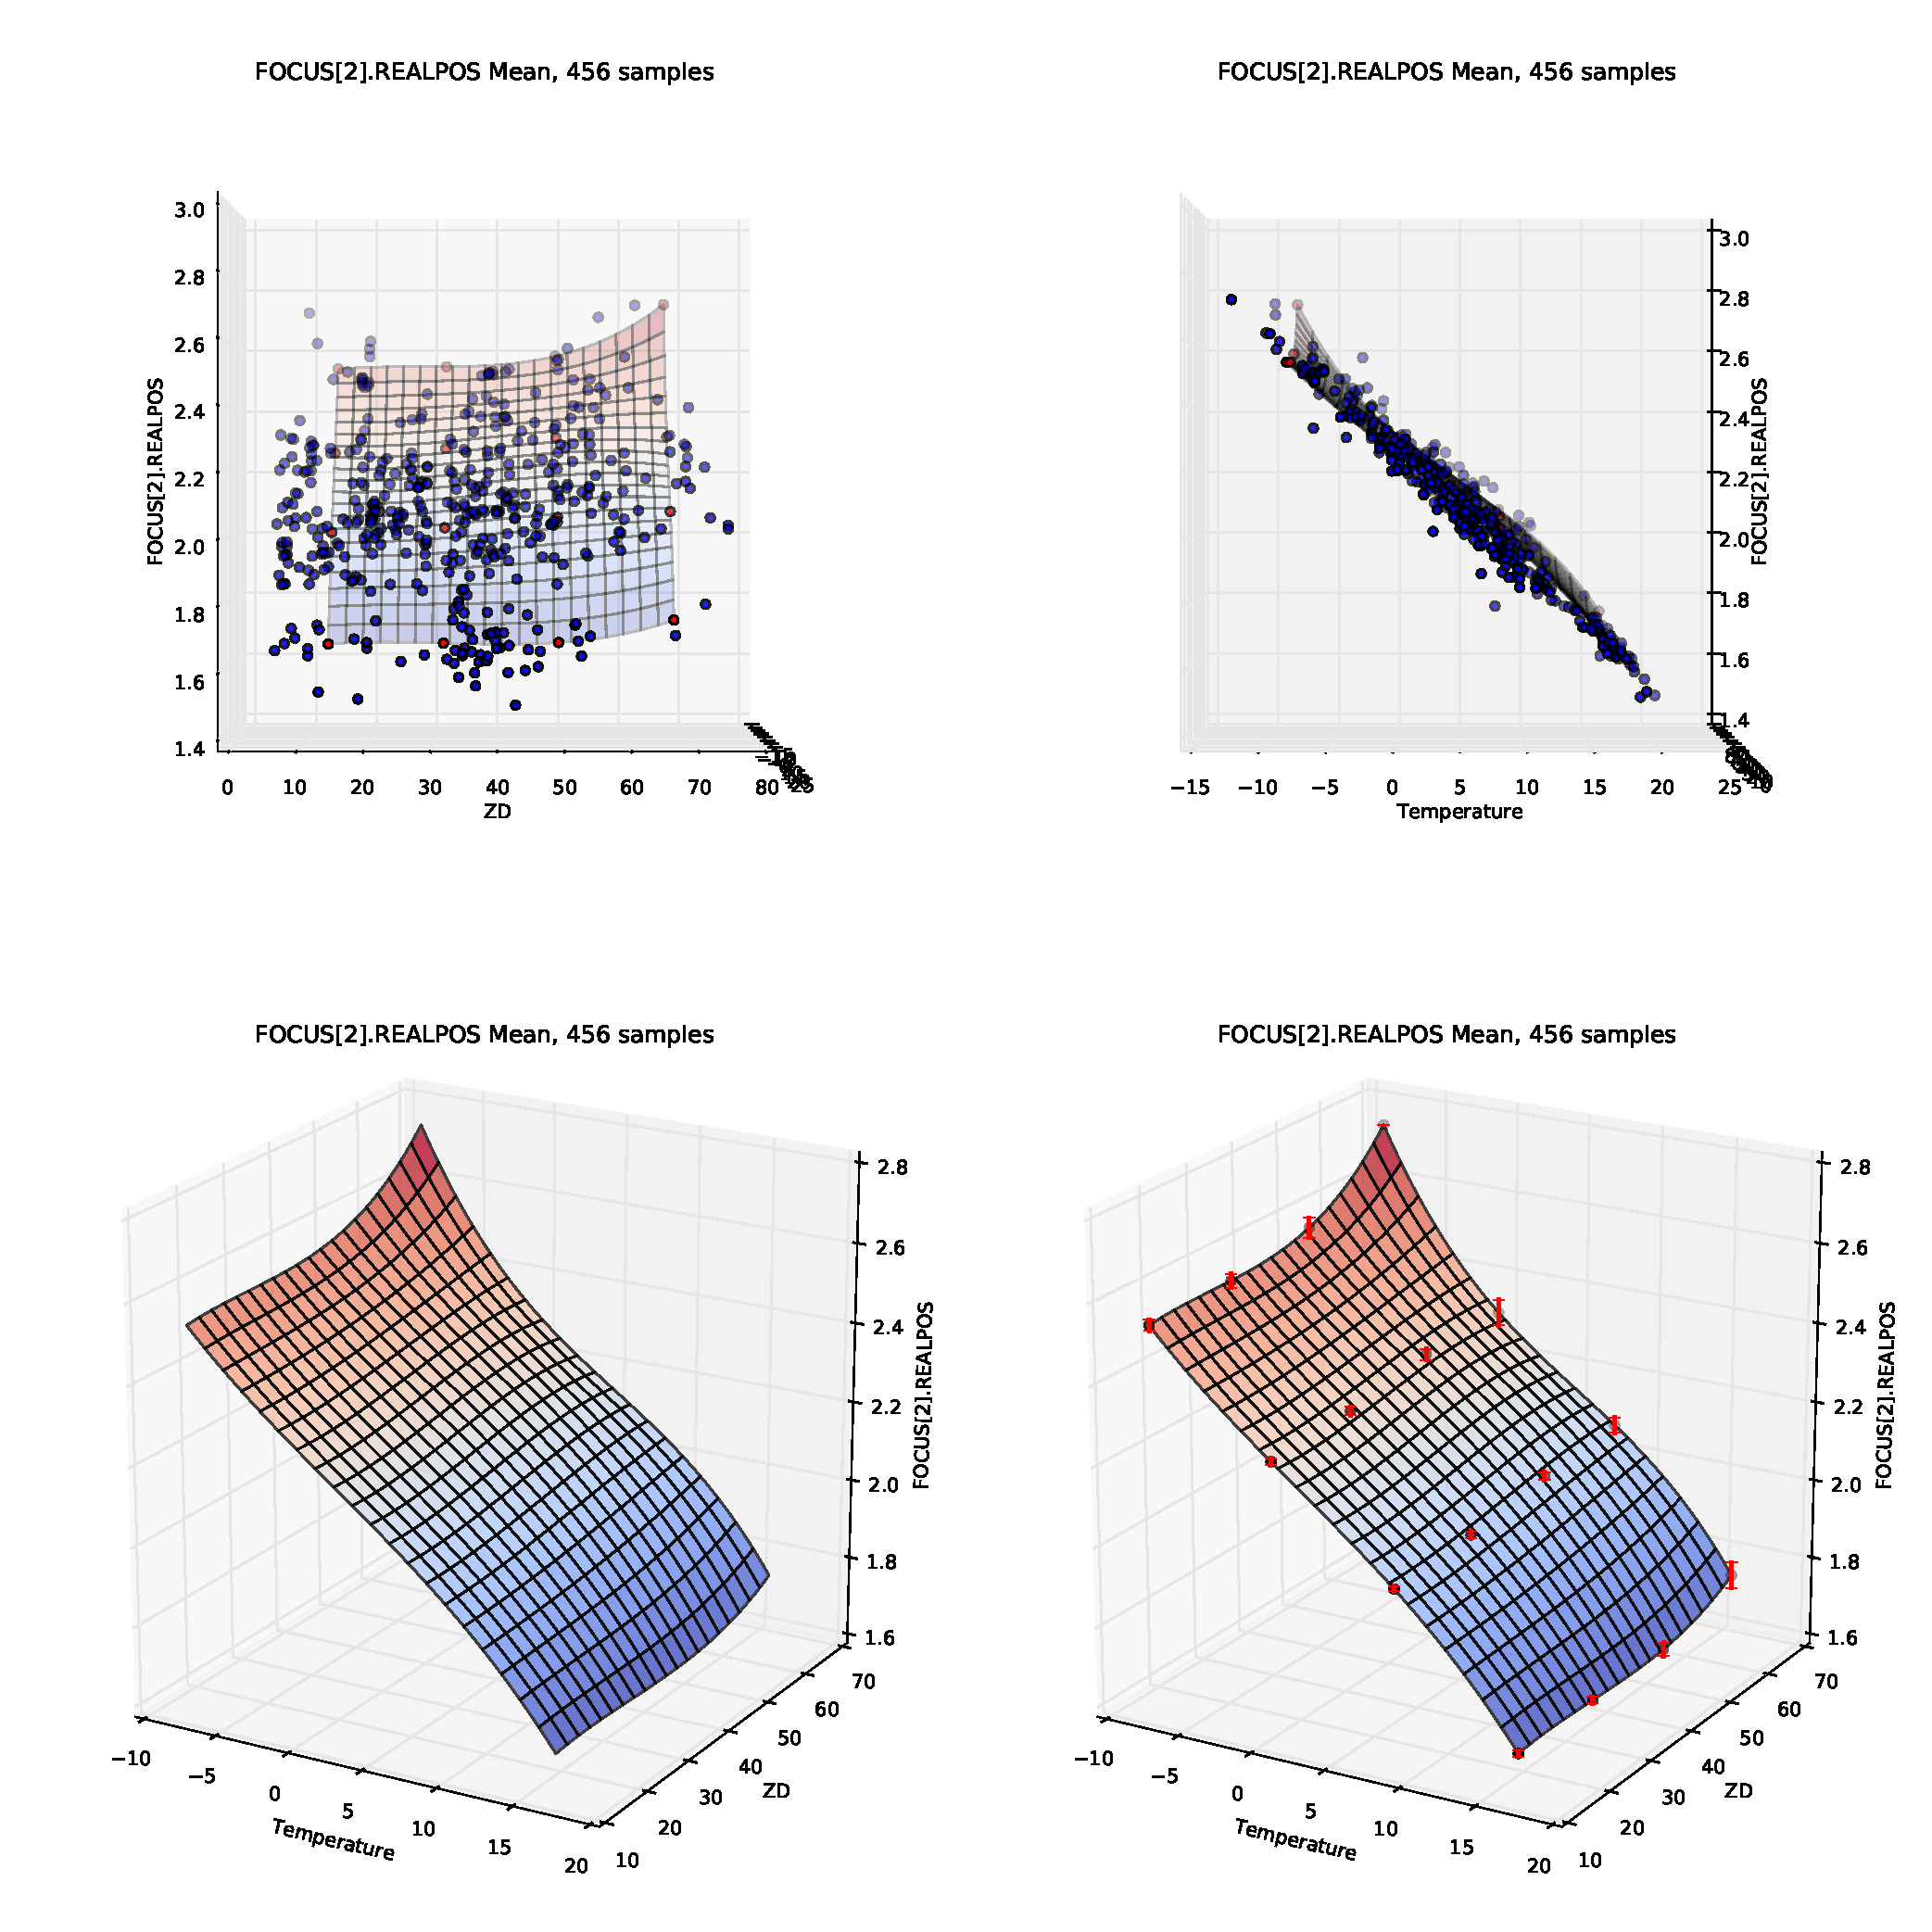
\includegraphics[scale=.44]{tsi_surf/POSITION_INSTRUMENTAL_FOCUS_2__REALPOS_mean.pdf}
	\caption[Mean Streu- und Flächenplot des Sekundärspiegels]{Mean Streu- und Flächenplot des Sekundärspiegels}
    \label{foc_mean}
\end{figure}
\begin{figure}[H]
	\centering
	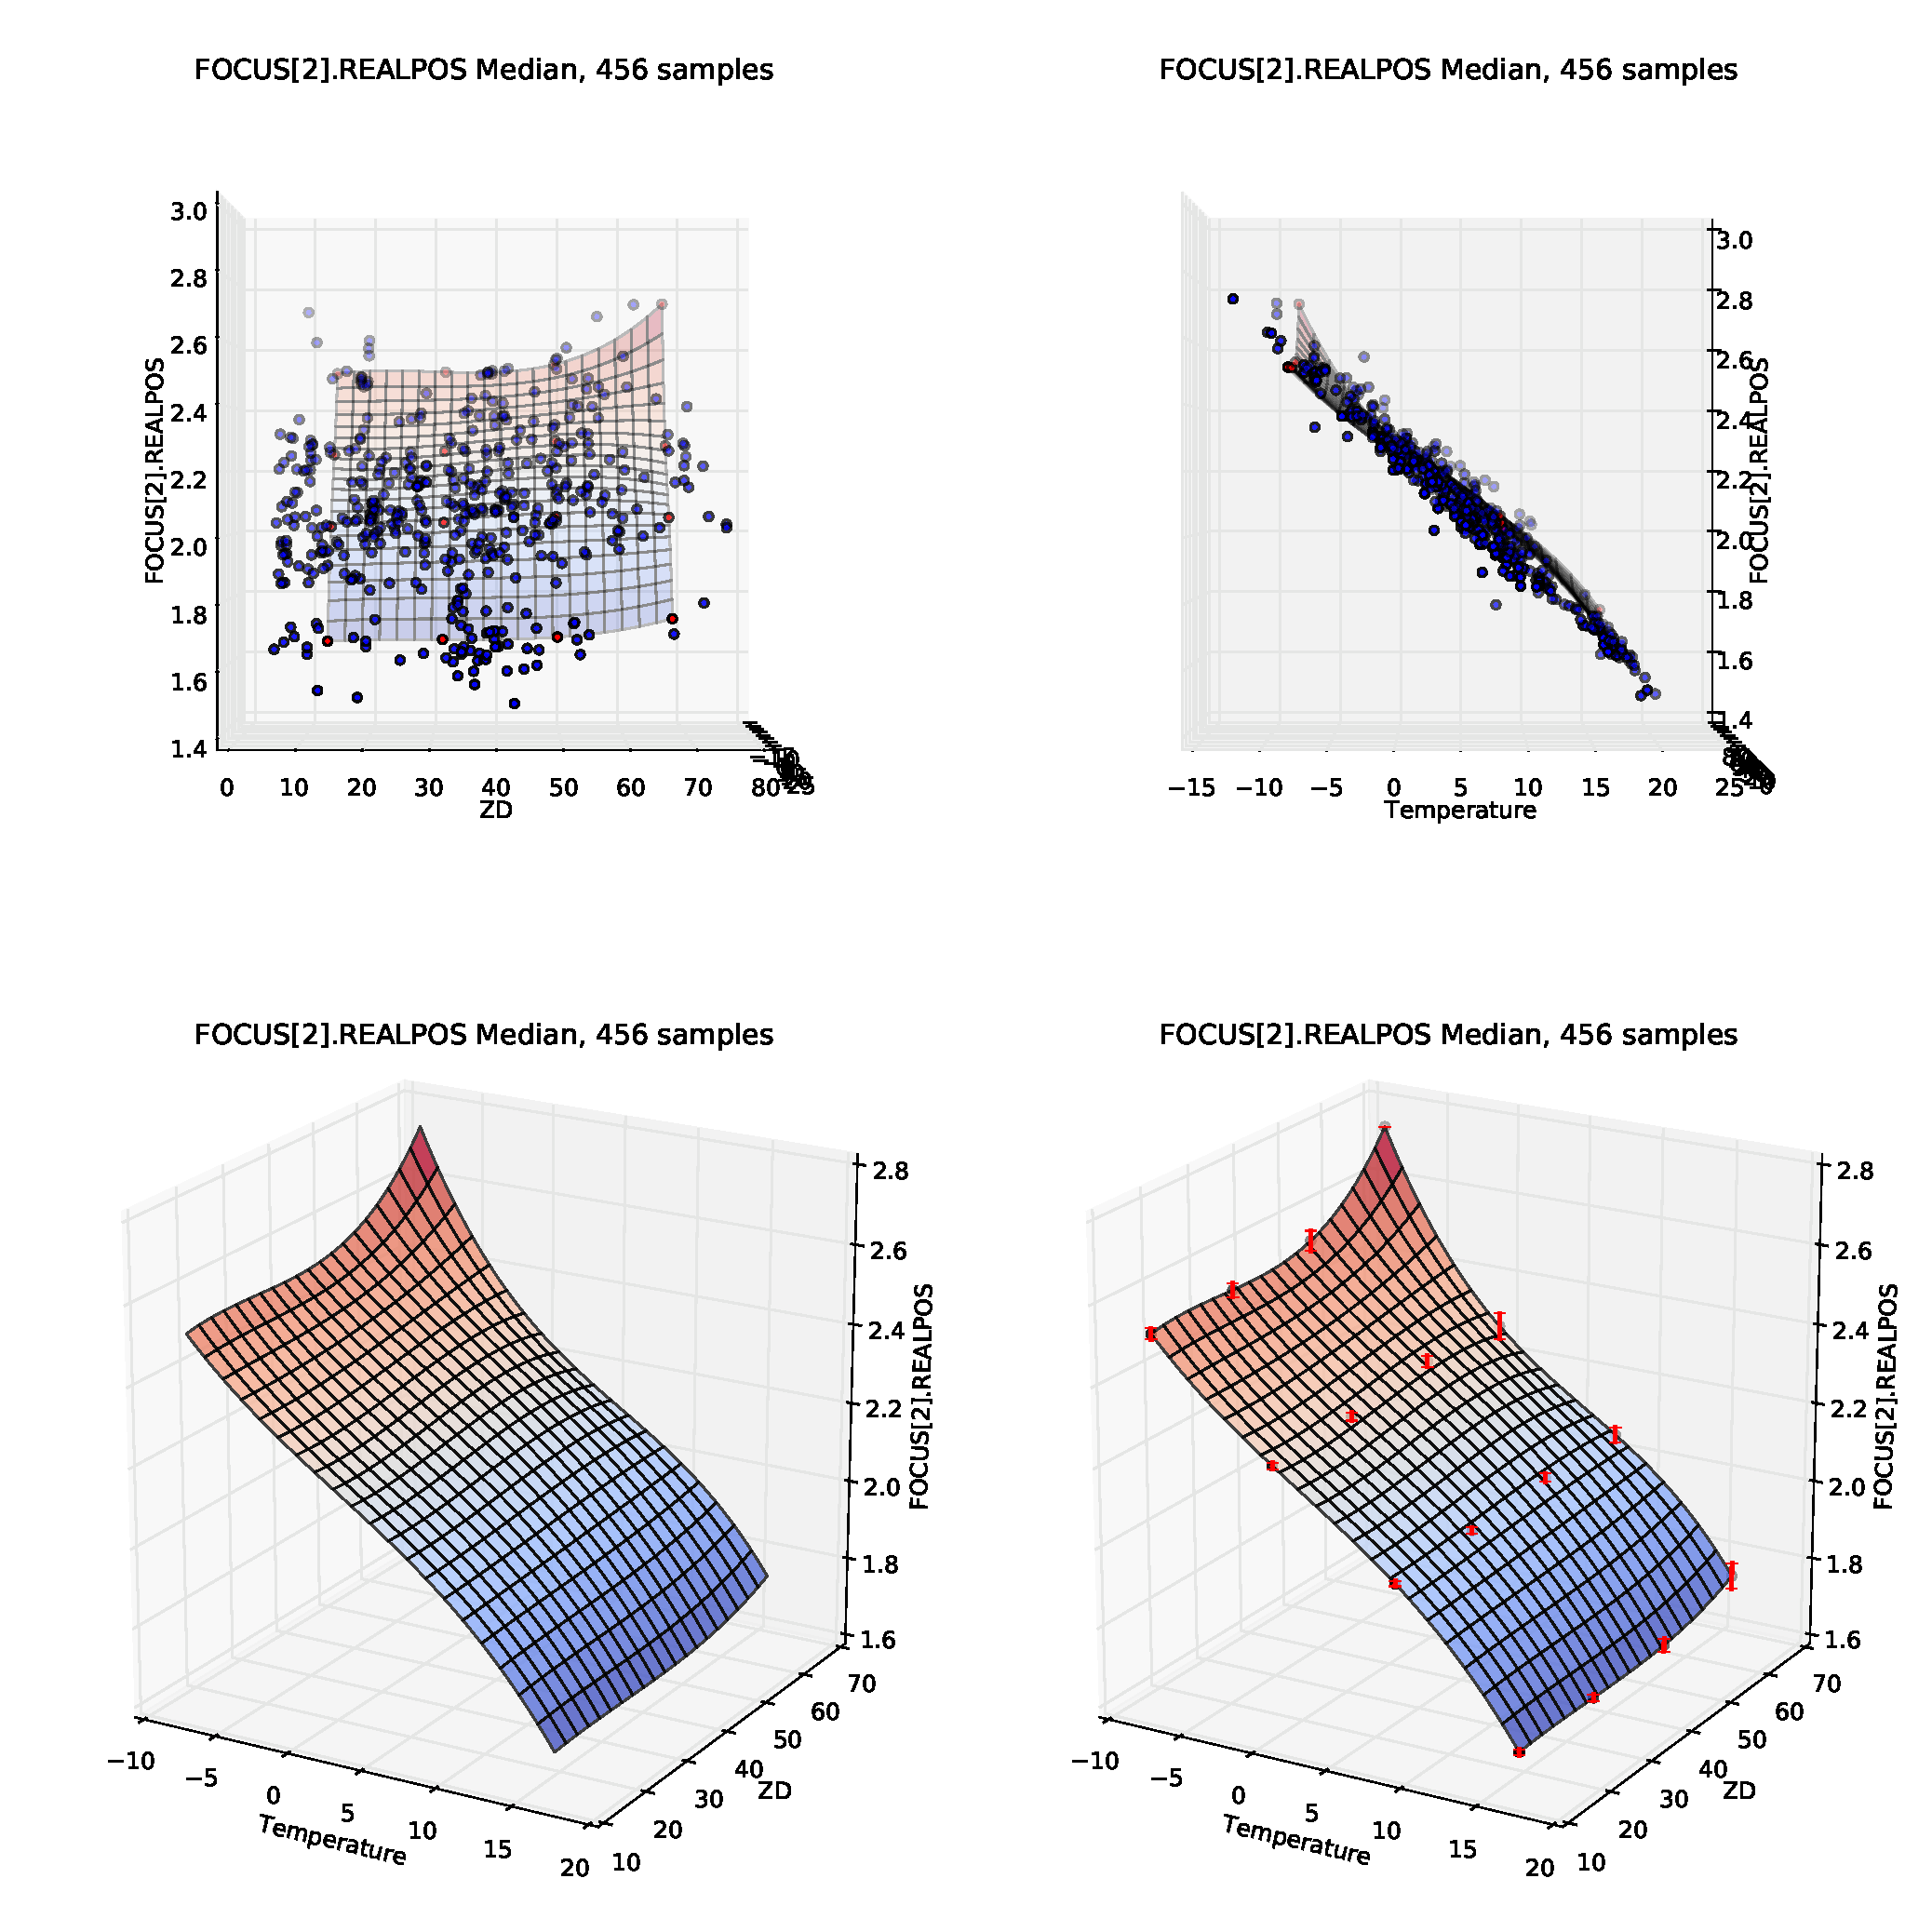
\includegraphics[scale=.44]{tsi_surf/POSITION_INSTRUMENTAL_FOCUS_2__REALPOS_med.pdf}
	\caption[Median Streu- und Flächenplot des Sekundärspiegels]{Median Streu- und Flächenplot des Sekundärspiegels}
    \label{foc_med}
\end{figure}
\begin{figure}[H]
	\centering
	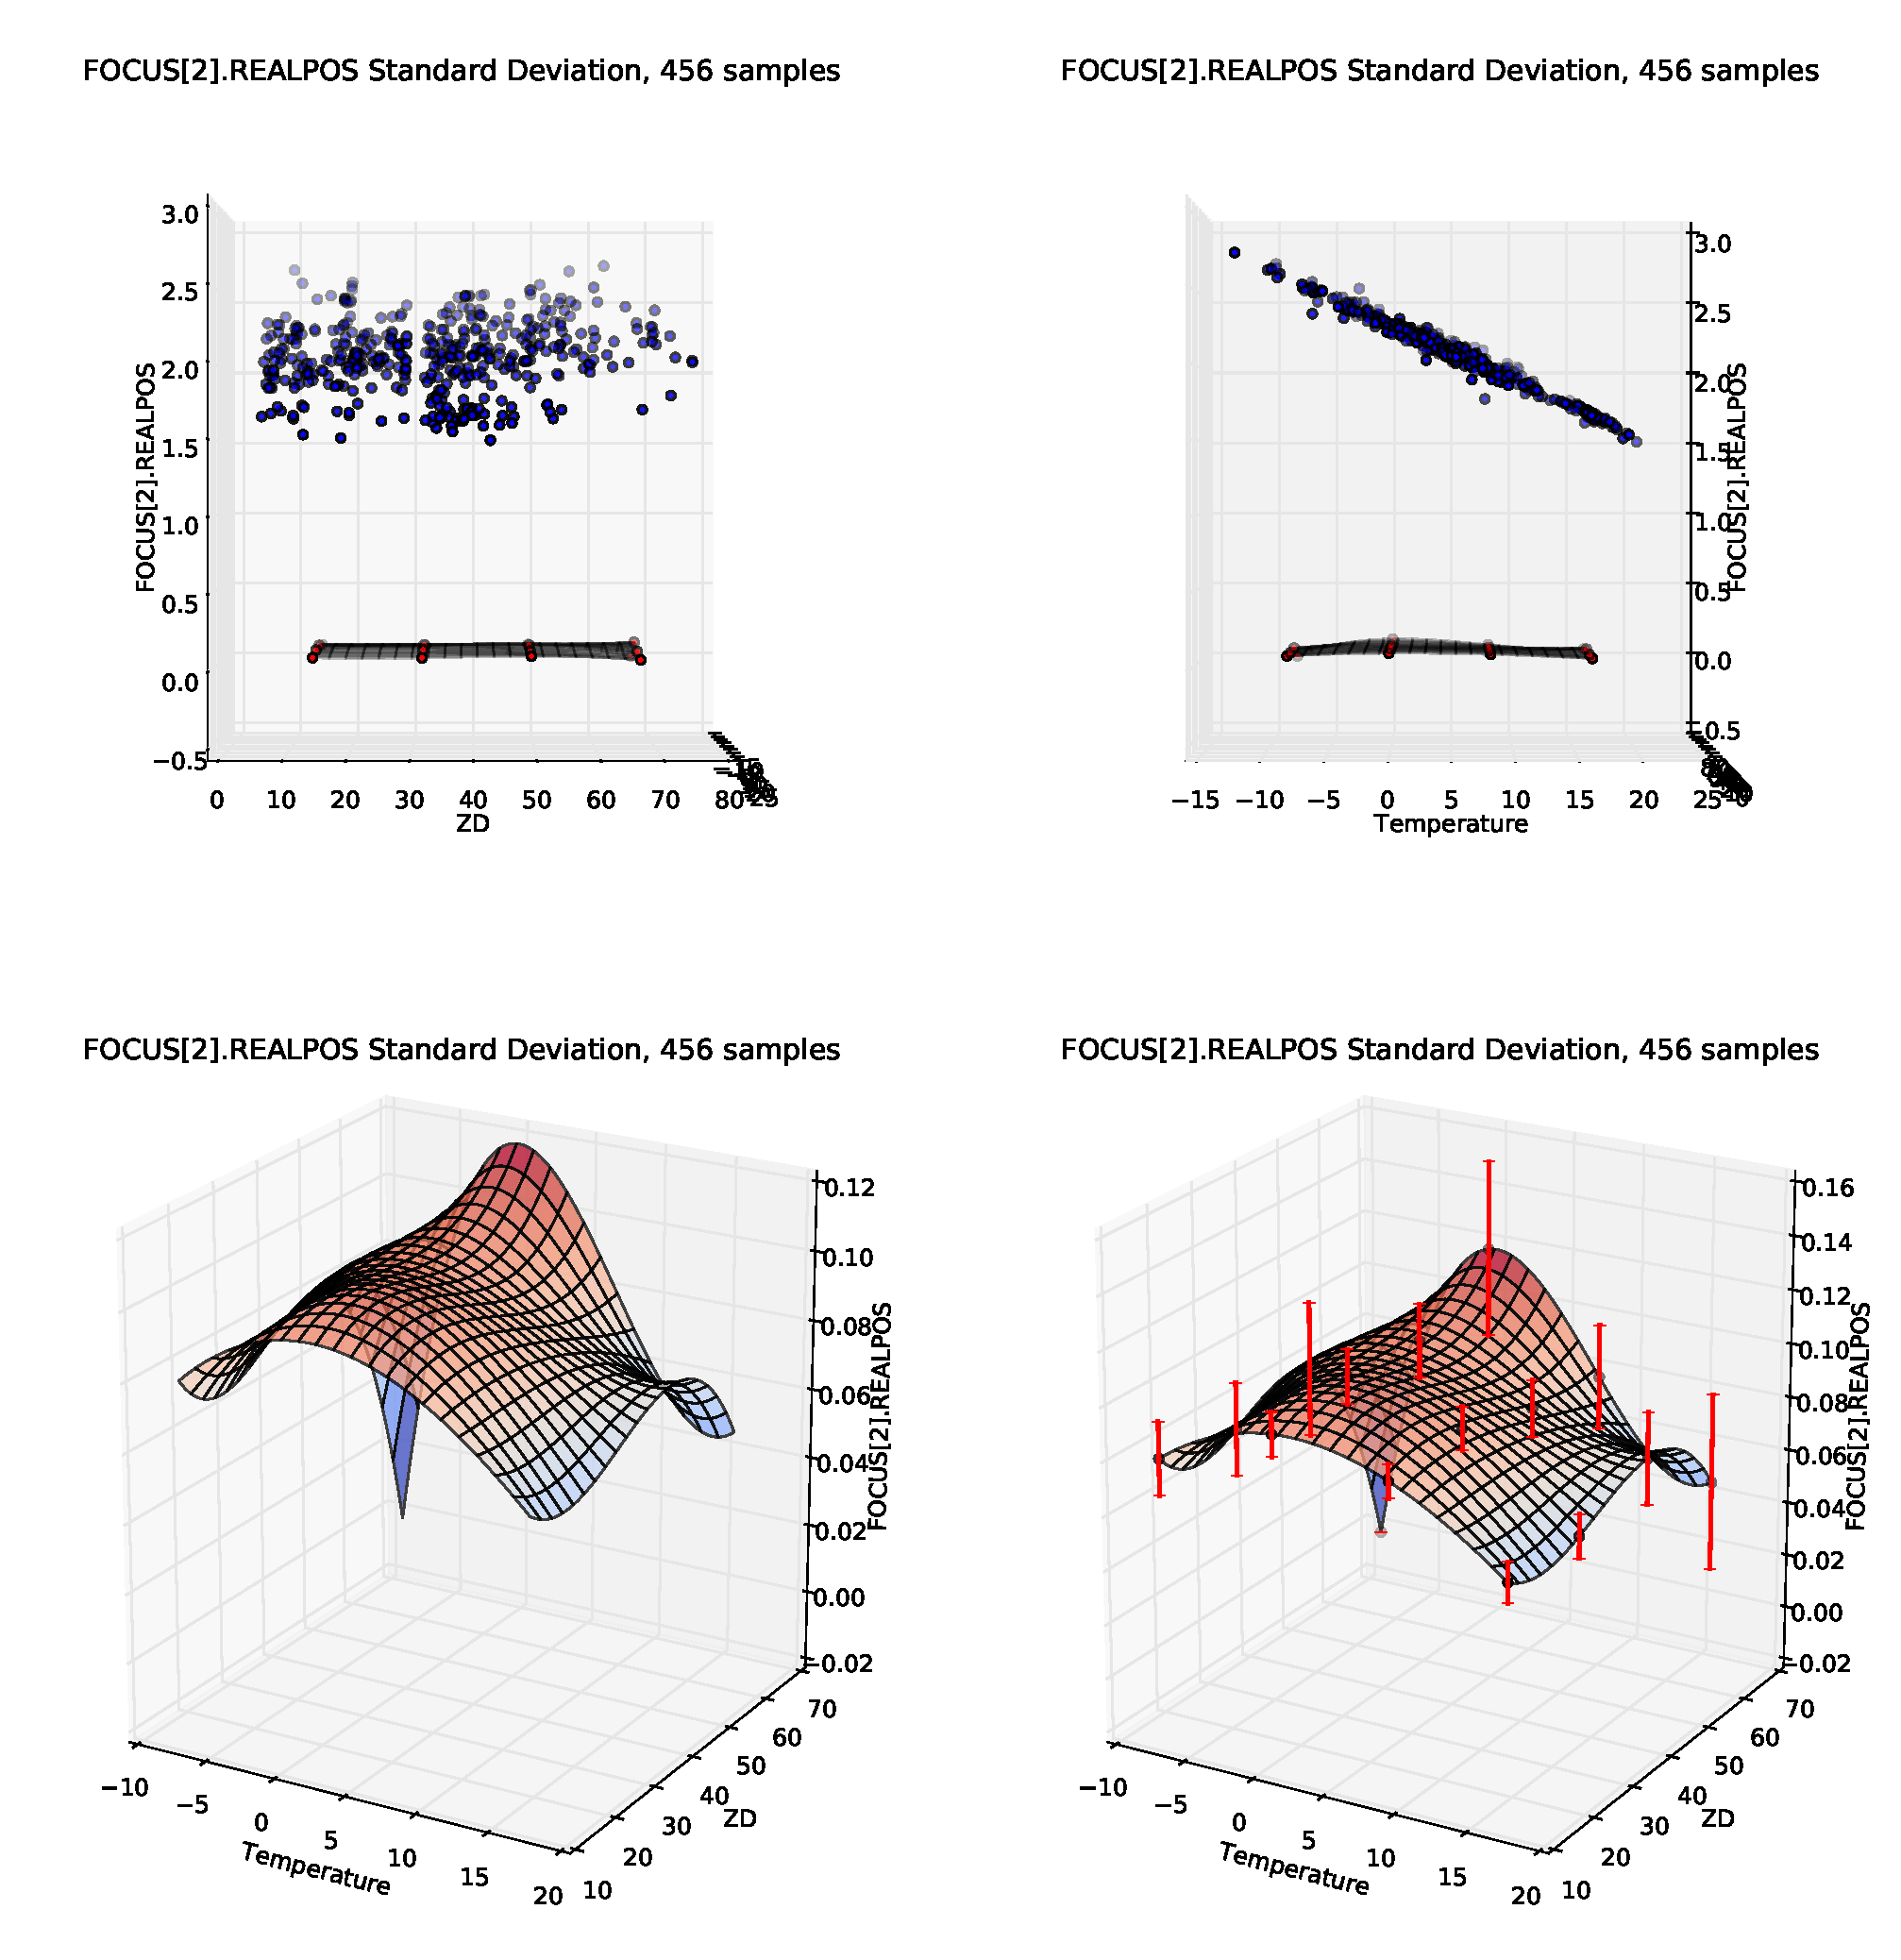
\includegraphics[scale=.44]{tsi_surf/POSITION_INSTRUMENTAL_FOCUS_2__REALPOS_std.pdf}
	\caption[Standardabweichung Streu- und Flächenplot des Sekundärspiegels]{Standardabweichung Streu- und Flächenplot des Sekundärspiegels}
    \label{foc_std}
\end{figure}
\begin{figure}[H]
	\centering
	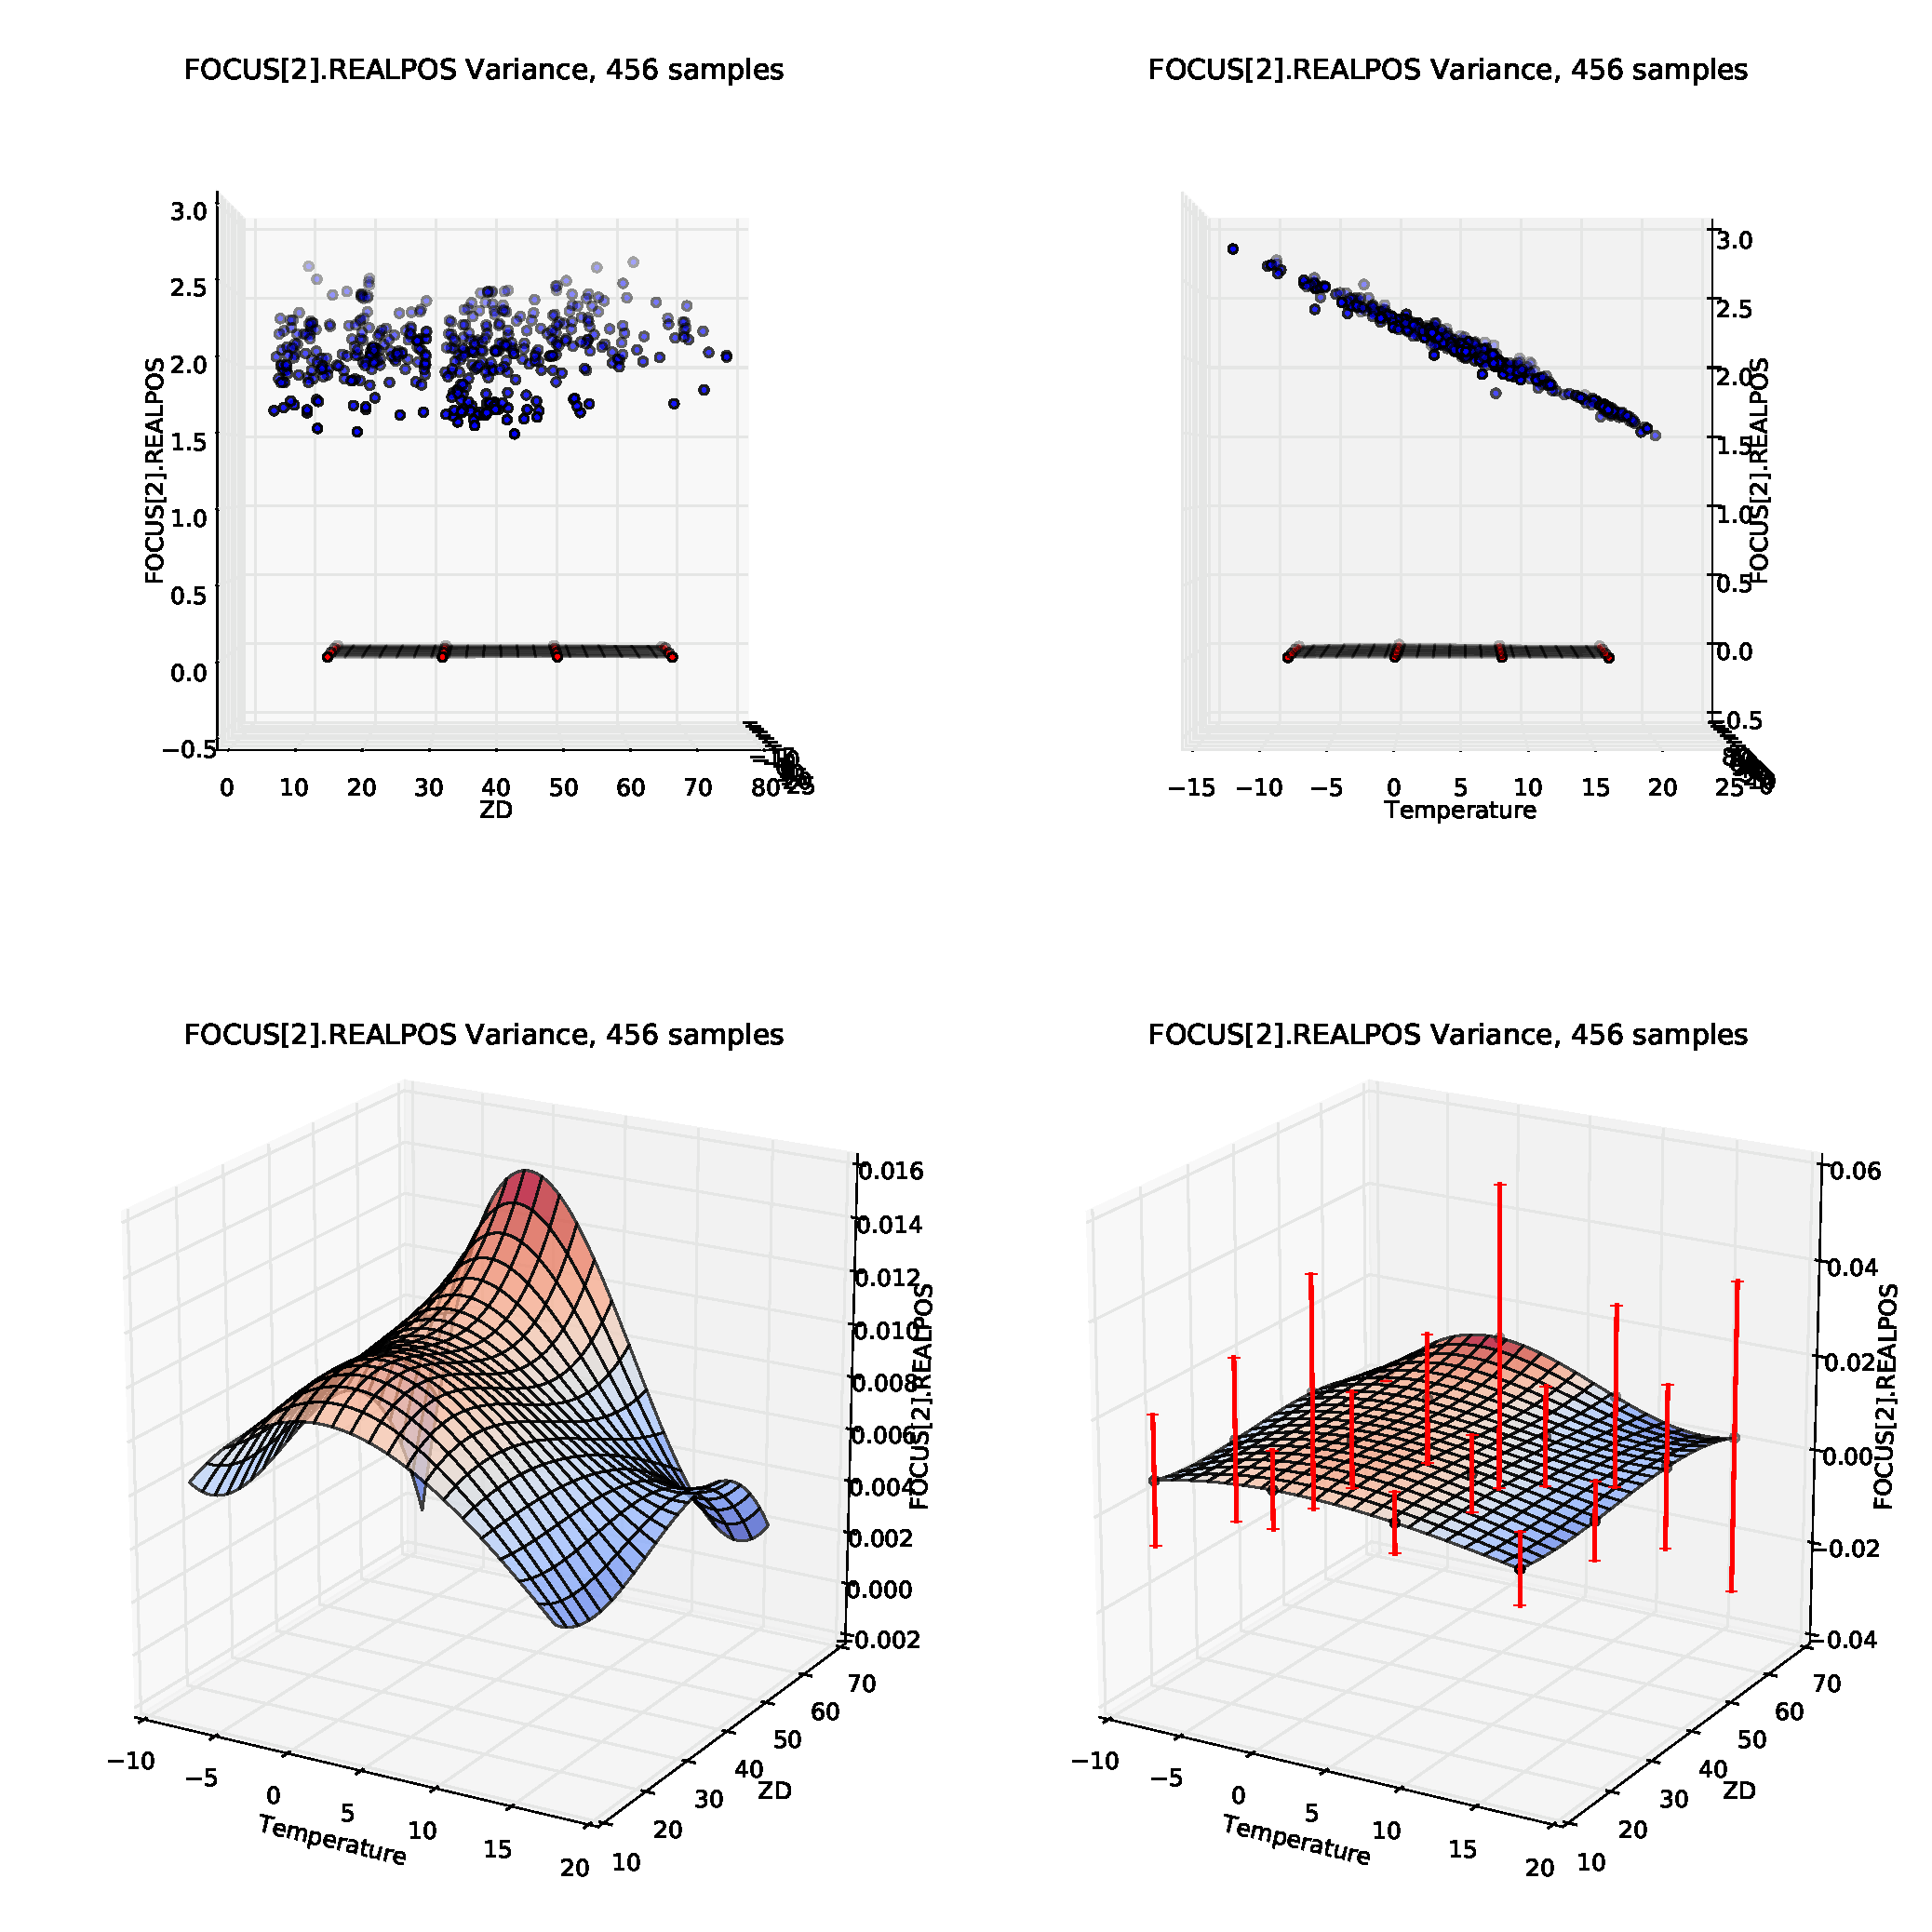
\includegraphics[scale=.44]{tsi_surf/POSITION_INSTRUMENTAL_FOCUS_2__REALPOS_var.pdf}
	\caption[Varianz Streu- und Flächenplot des Sekundärspiegels]{Varianz Streu- und Flächenplot des Sekundärspiegels}
    \label{foc_var}
\end{figure}

\section{Transinformation Korrelationsmatrizen}

\begin{figure}[H]
	\centering
	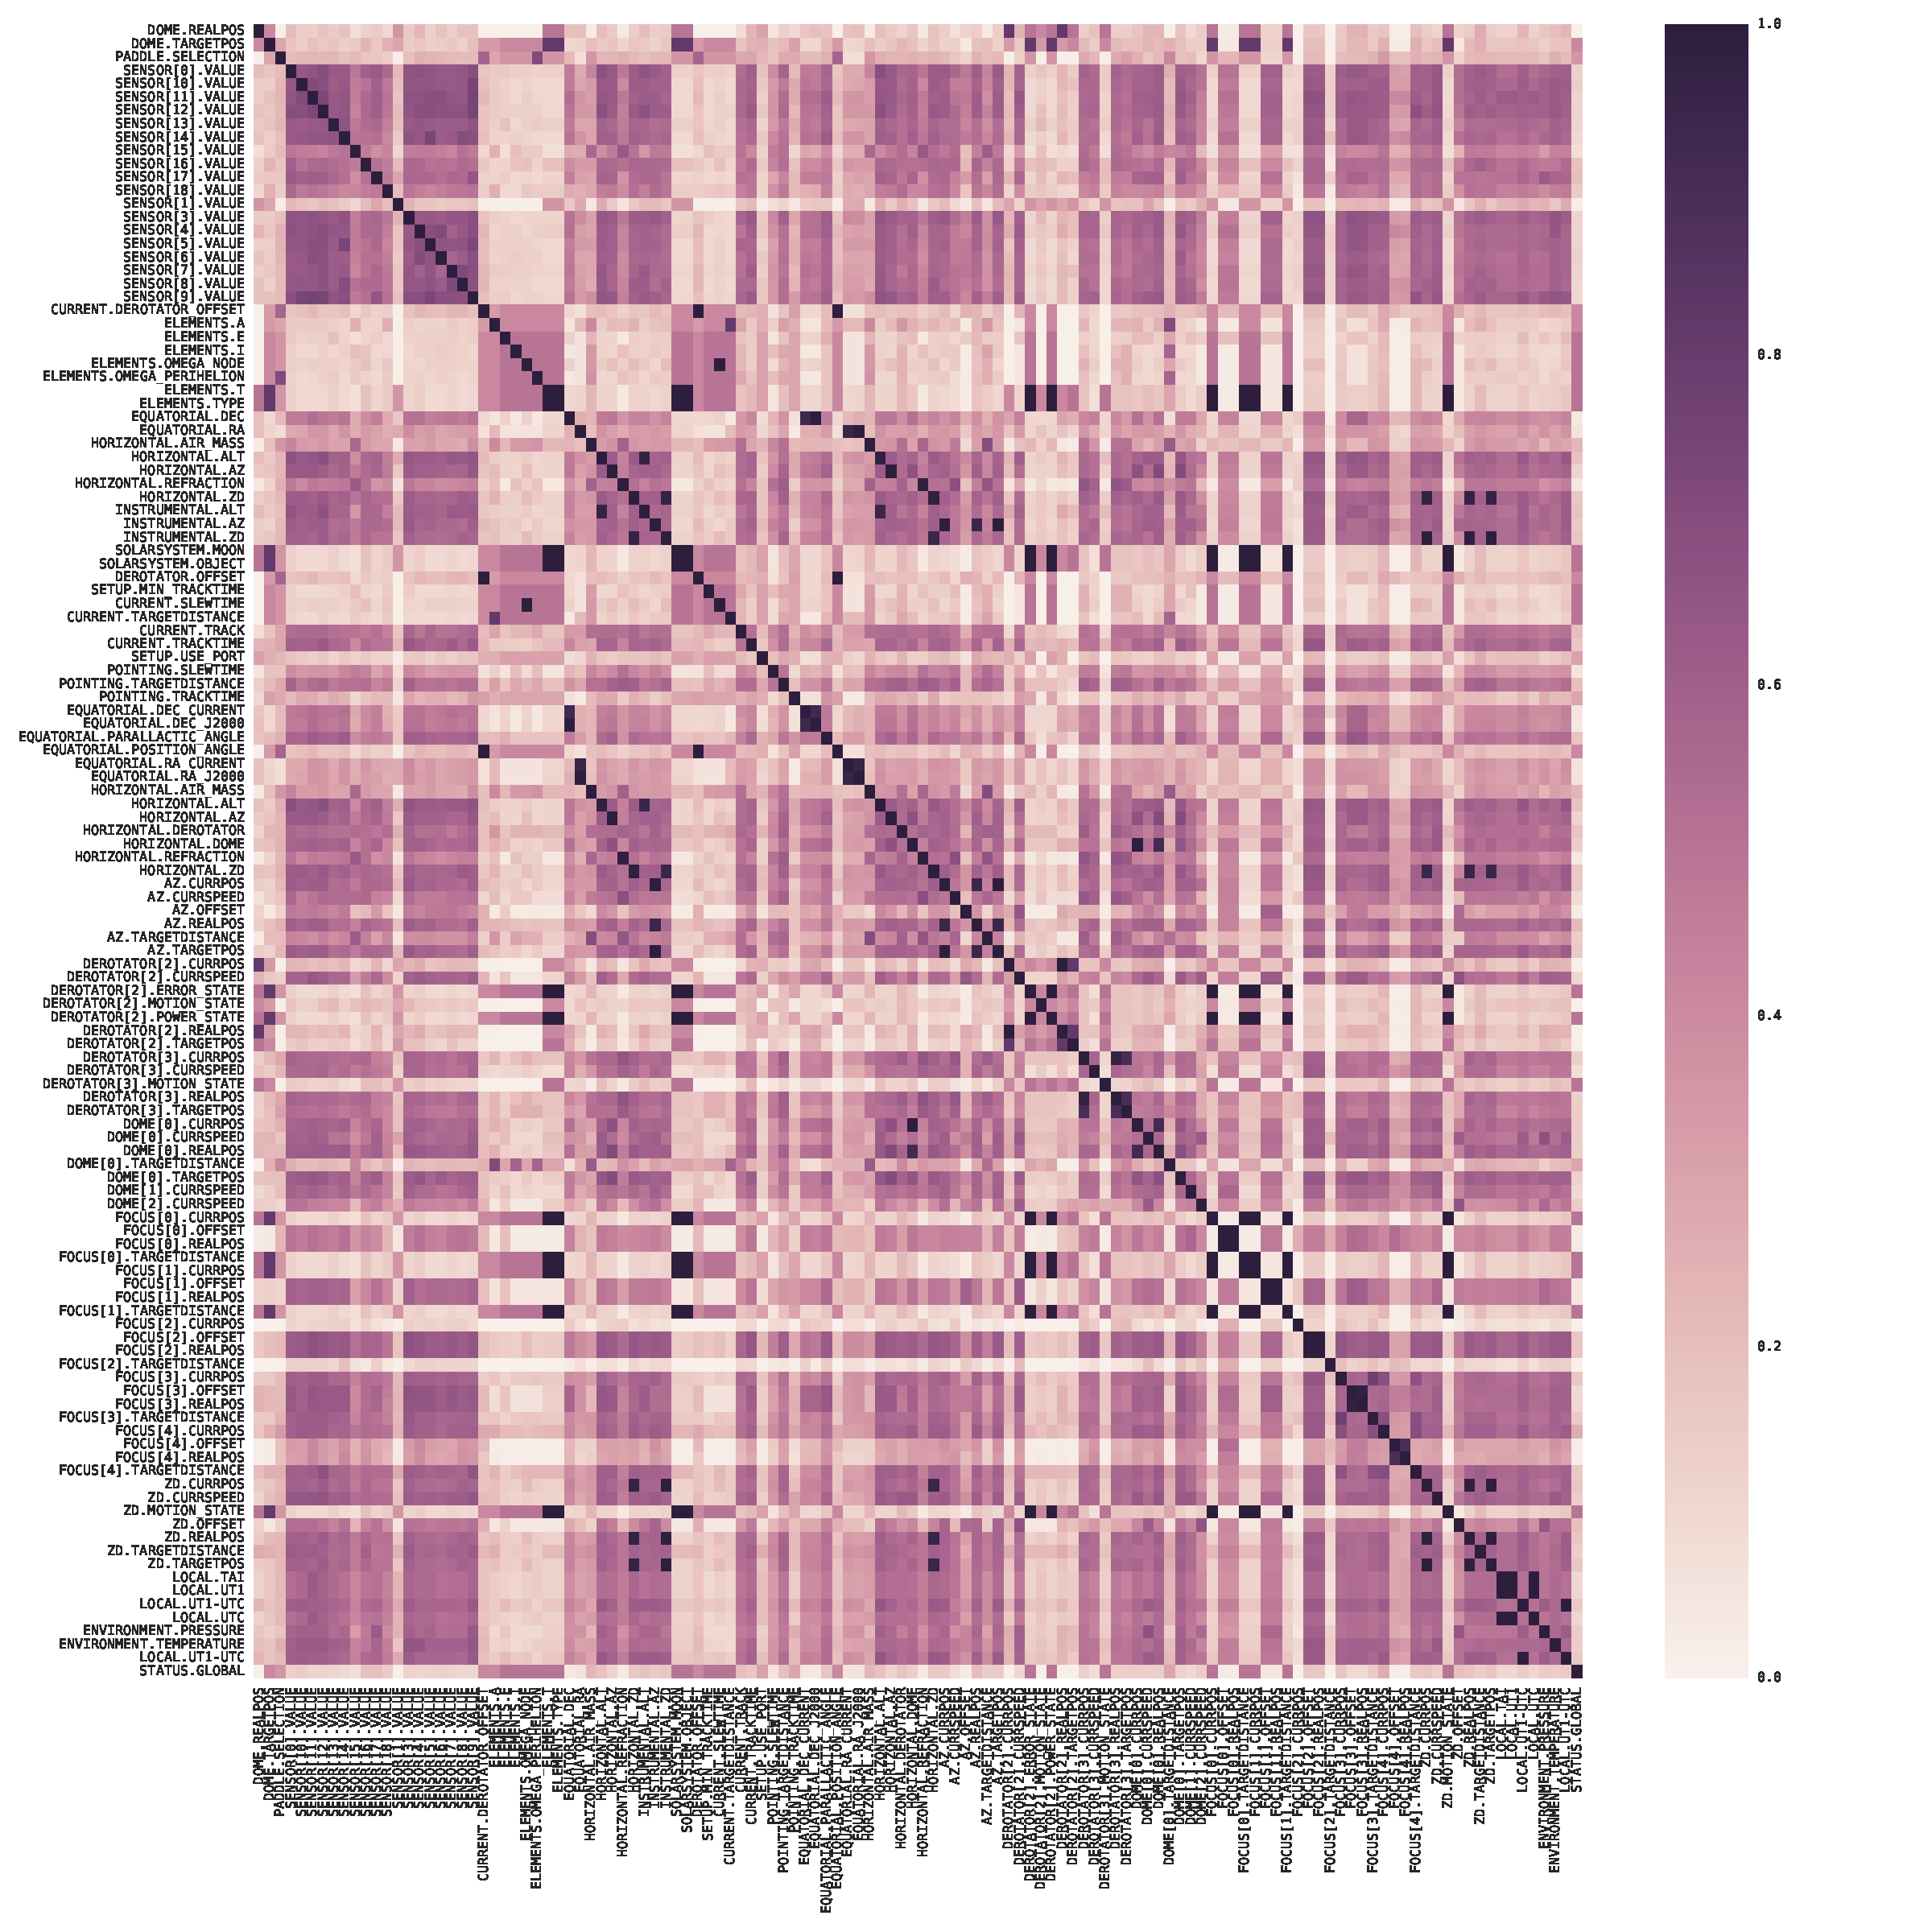
\includegraphics[scale=.44]{heatmaps/tsi.pdf}
	\caption[Heatmap der Transinformation Korrelationsmatrix der TSI-Parameter]{Heatmap der Transinformation Korrelationsmatrix der TSI-Parameter}
    \label{heatmap_tsi}
\end{figure}
\begin{figure}[H]
	\centering
	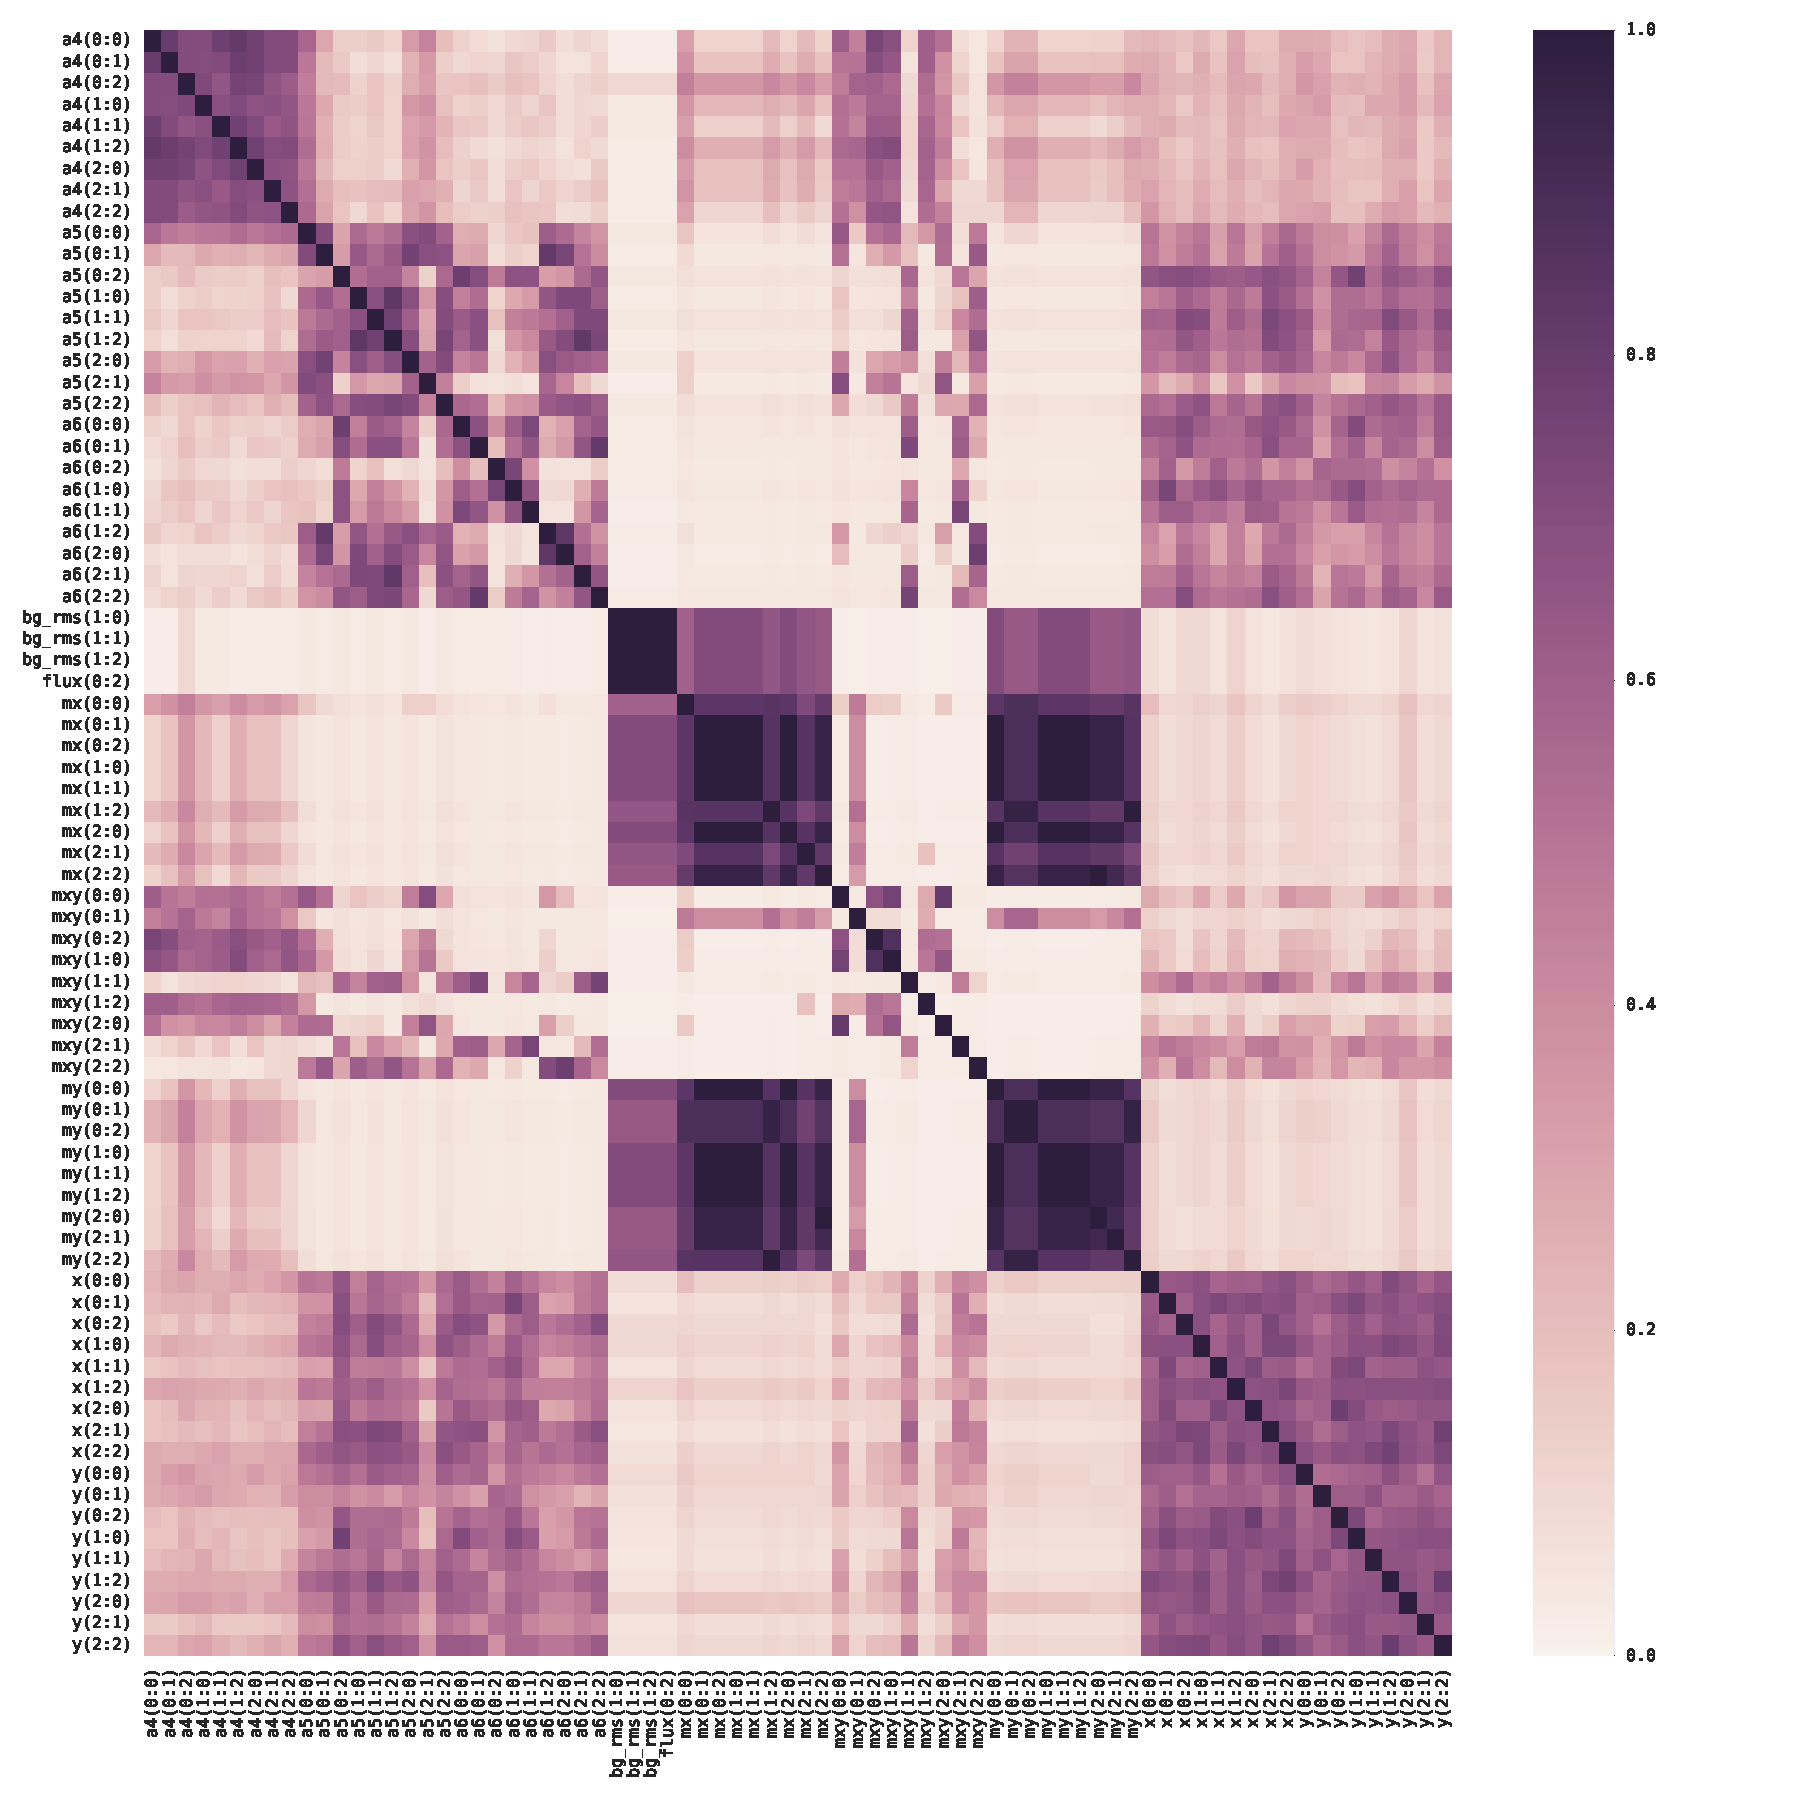
\includegraphics[scale=.58]{heatmaps/psf.pdf}
	\caption[Heatmap der Transinformation Korrelationsmatrix der PSF-Parameter]{Heatmap der Transinformation Korrelationsmatrix der PSF-Parameter}
    \label{heatmap_psf}
\end{figure}
\begin{figure}[H]
	\centering
	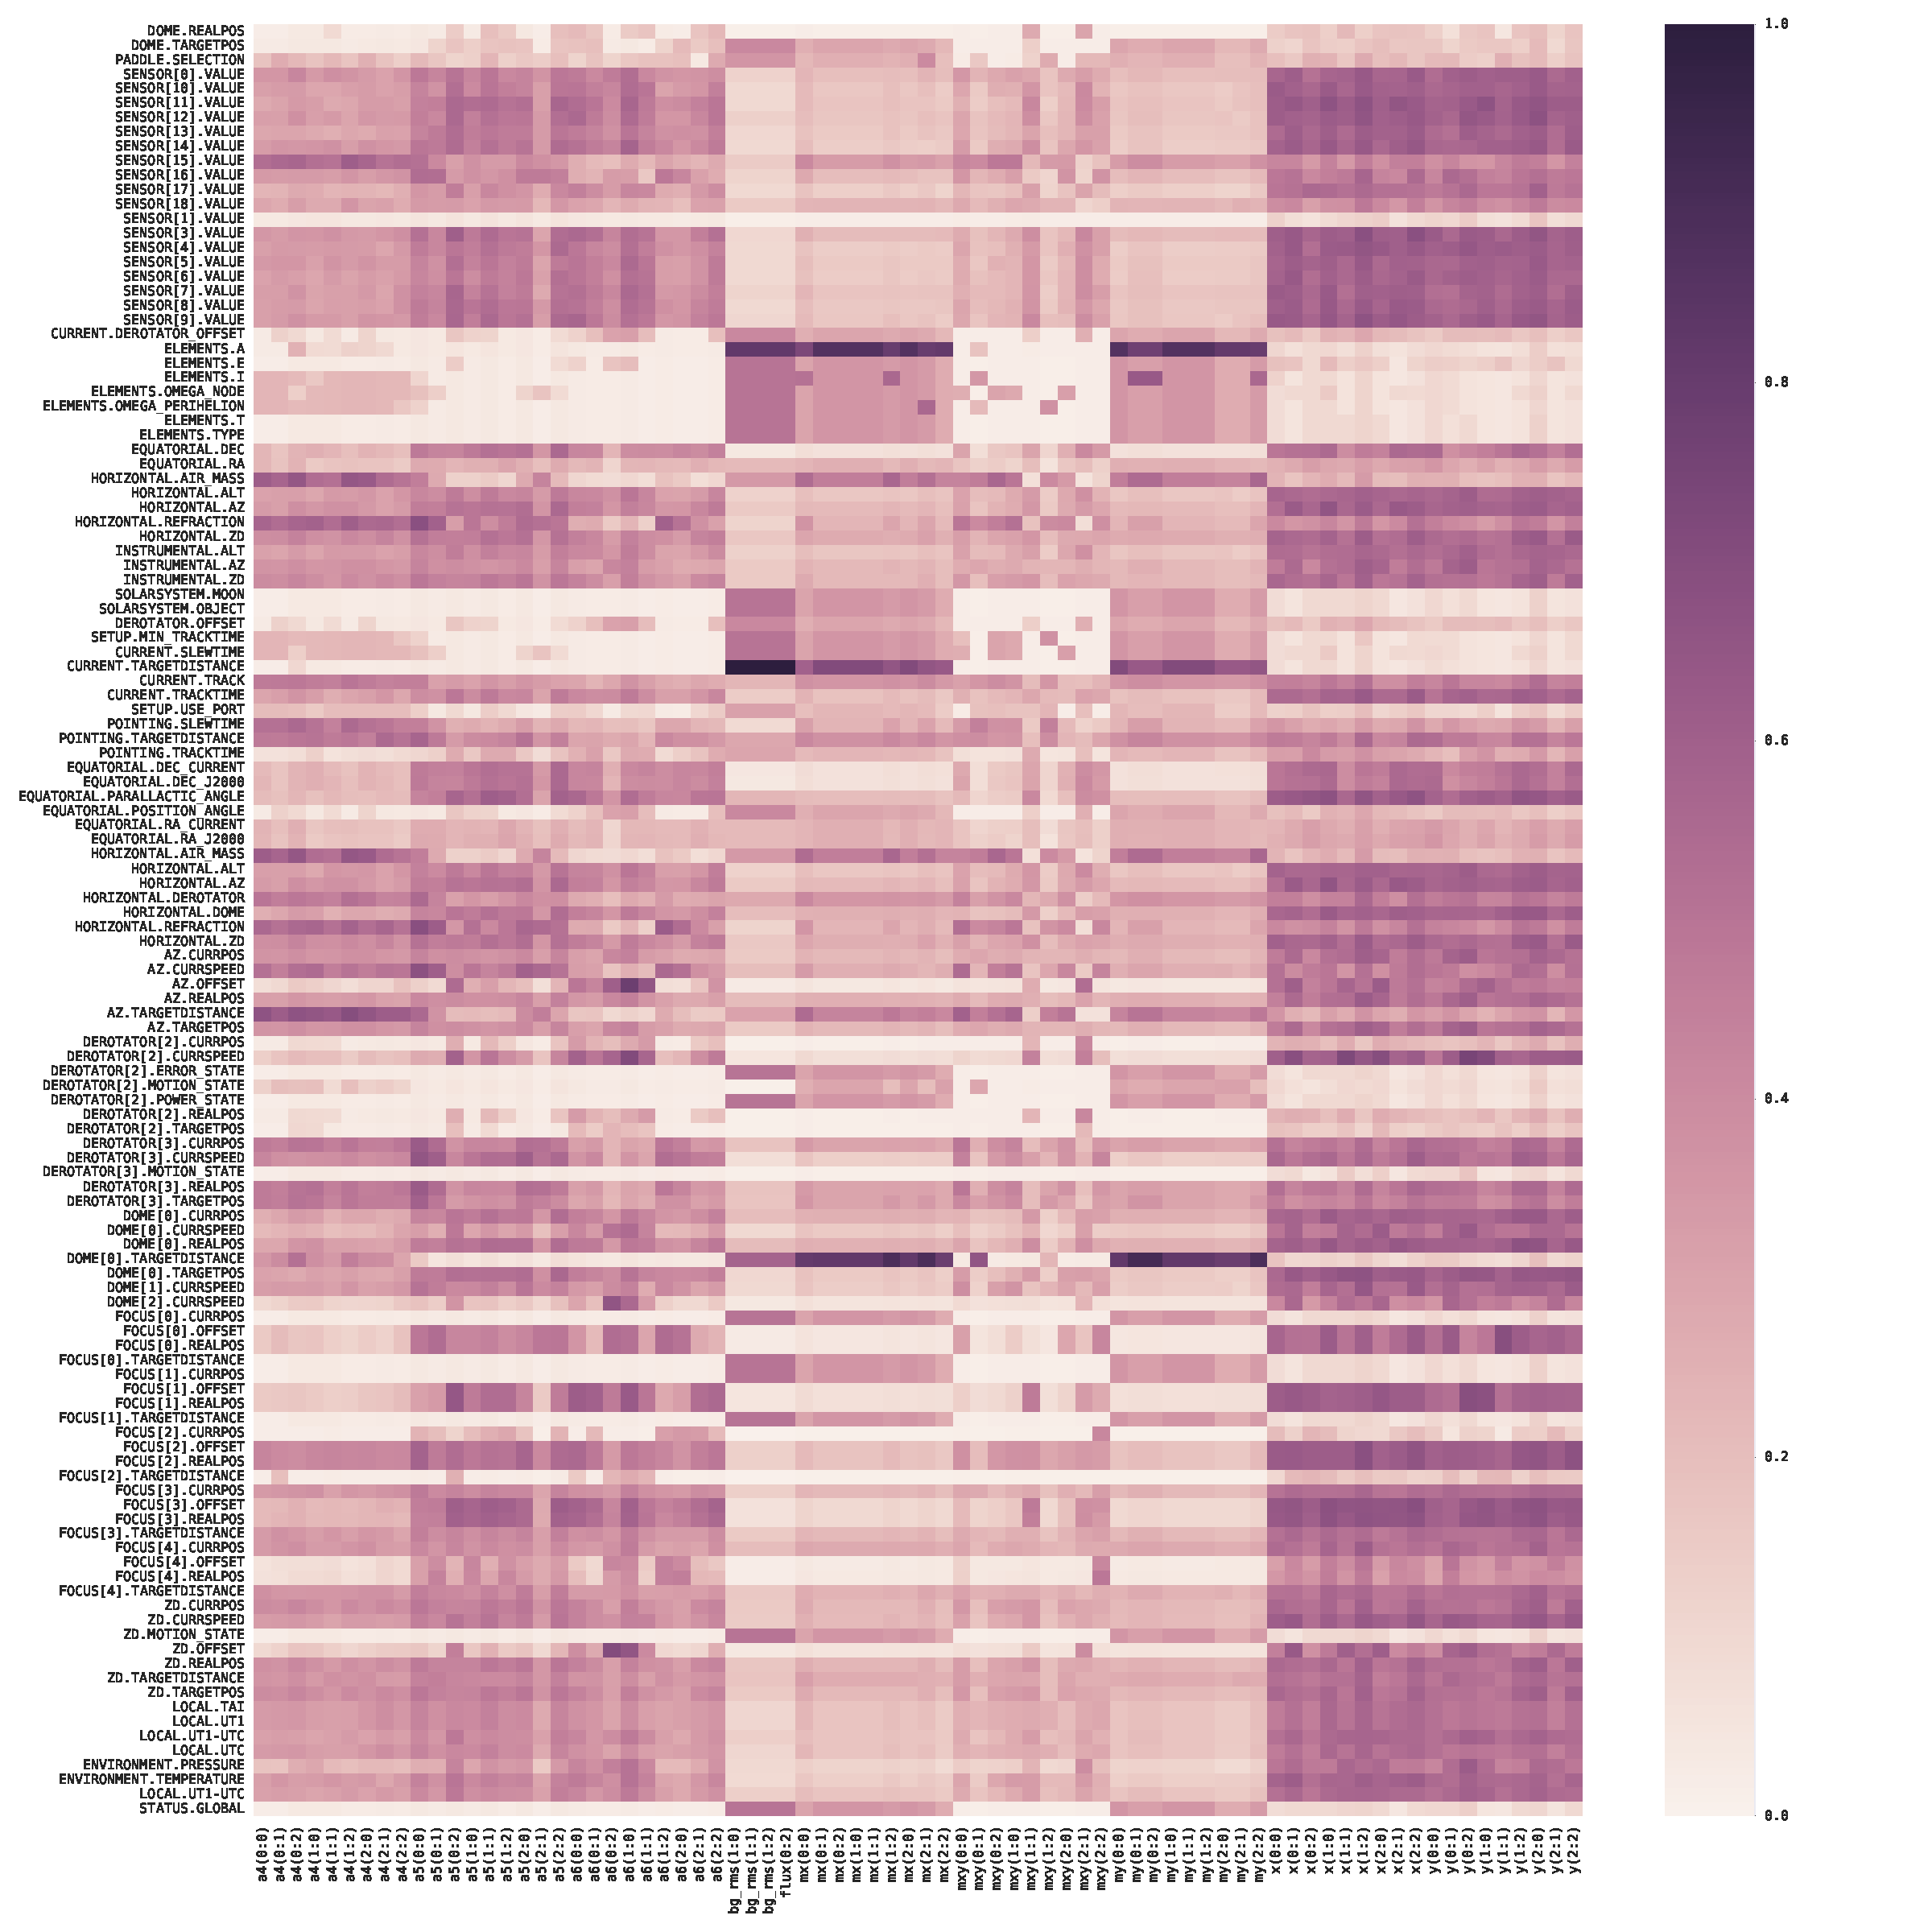
\includegraphics[scale=.44]{heatmaps/psf_tsi.pdf}
	\caption[Heatmap der Transinformation Korrelationsmatrix zwischen PSF- und TSI-Parametern]{Heatmap der Transinformation Korrelationsmatrix zwischen PSF- und TSI-Parametern}
    \label{heatmap_psf_tsi}
\end{figure}

\section{Windgeschwindigkeit, Windrichtung und PSF-Parameter}
\begin{figure}[H]
	\centering
	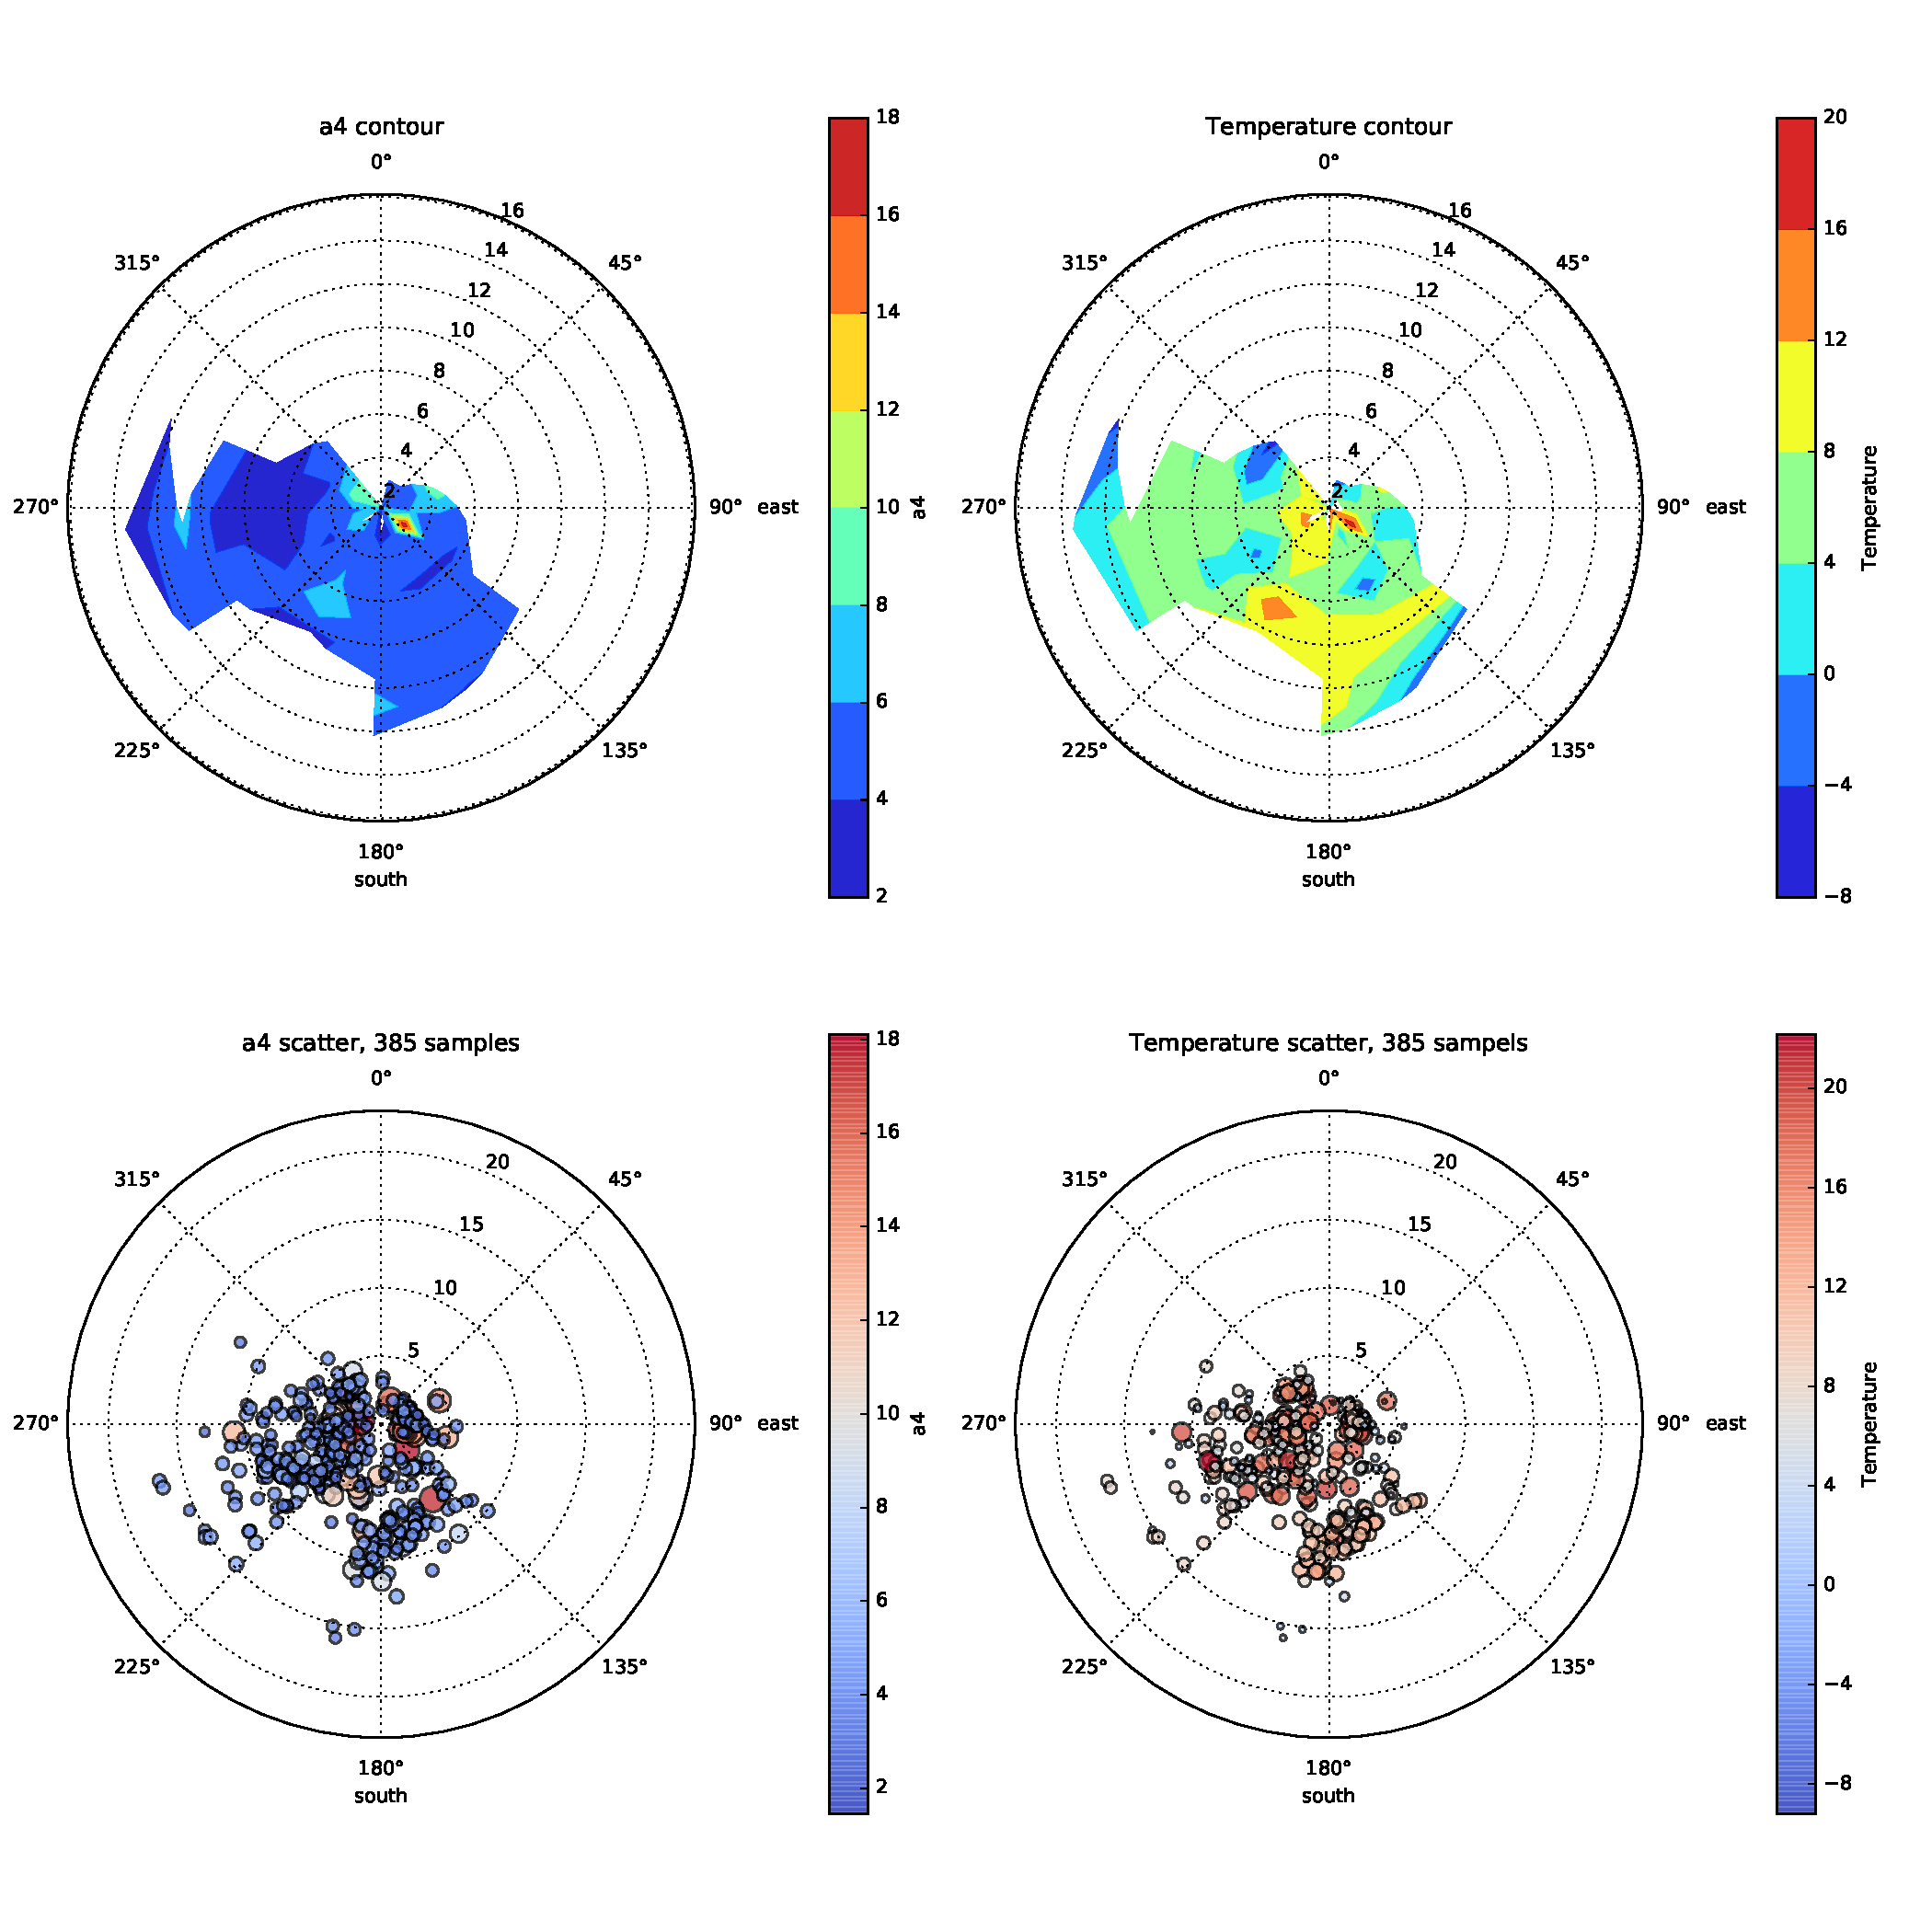
\includegraphics[scale=.46]{wind/wind_a4}
	\caption[Polarplot Windgeschwindigkeit, Windrichtung und $A_4$]{Polarplot Windgeschwindigkeit, Windrichtung und $A_4$}
    \label{wind_a4}
\end{figure}
\begin{figure}[H]
	\centering
	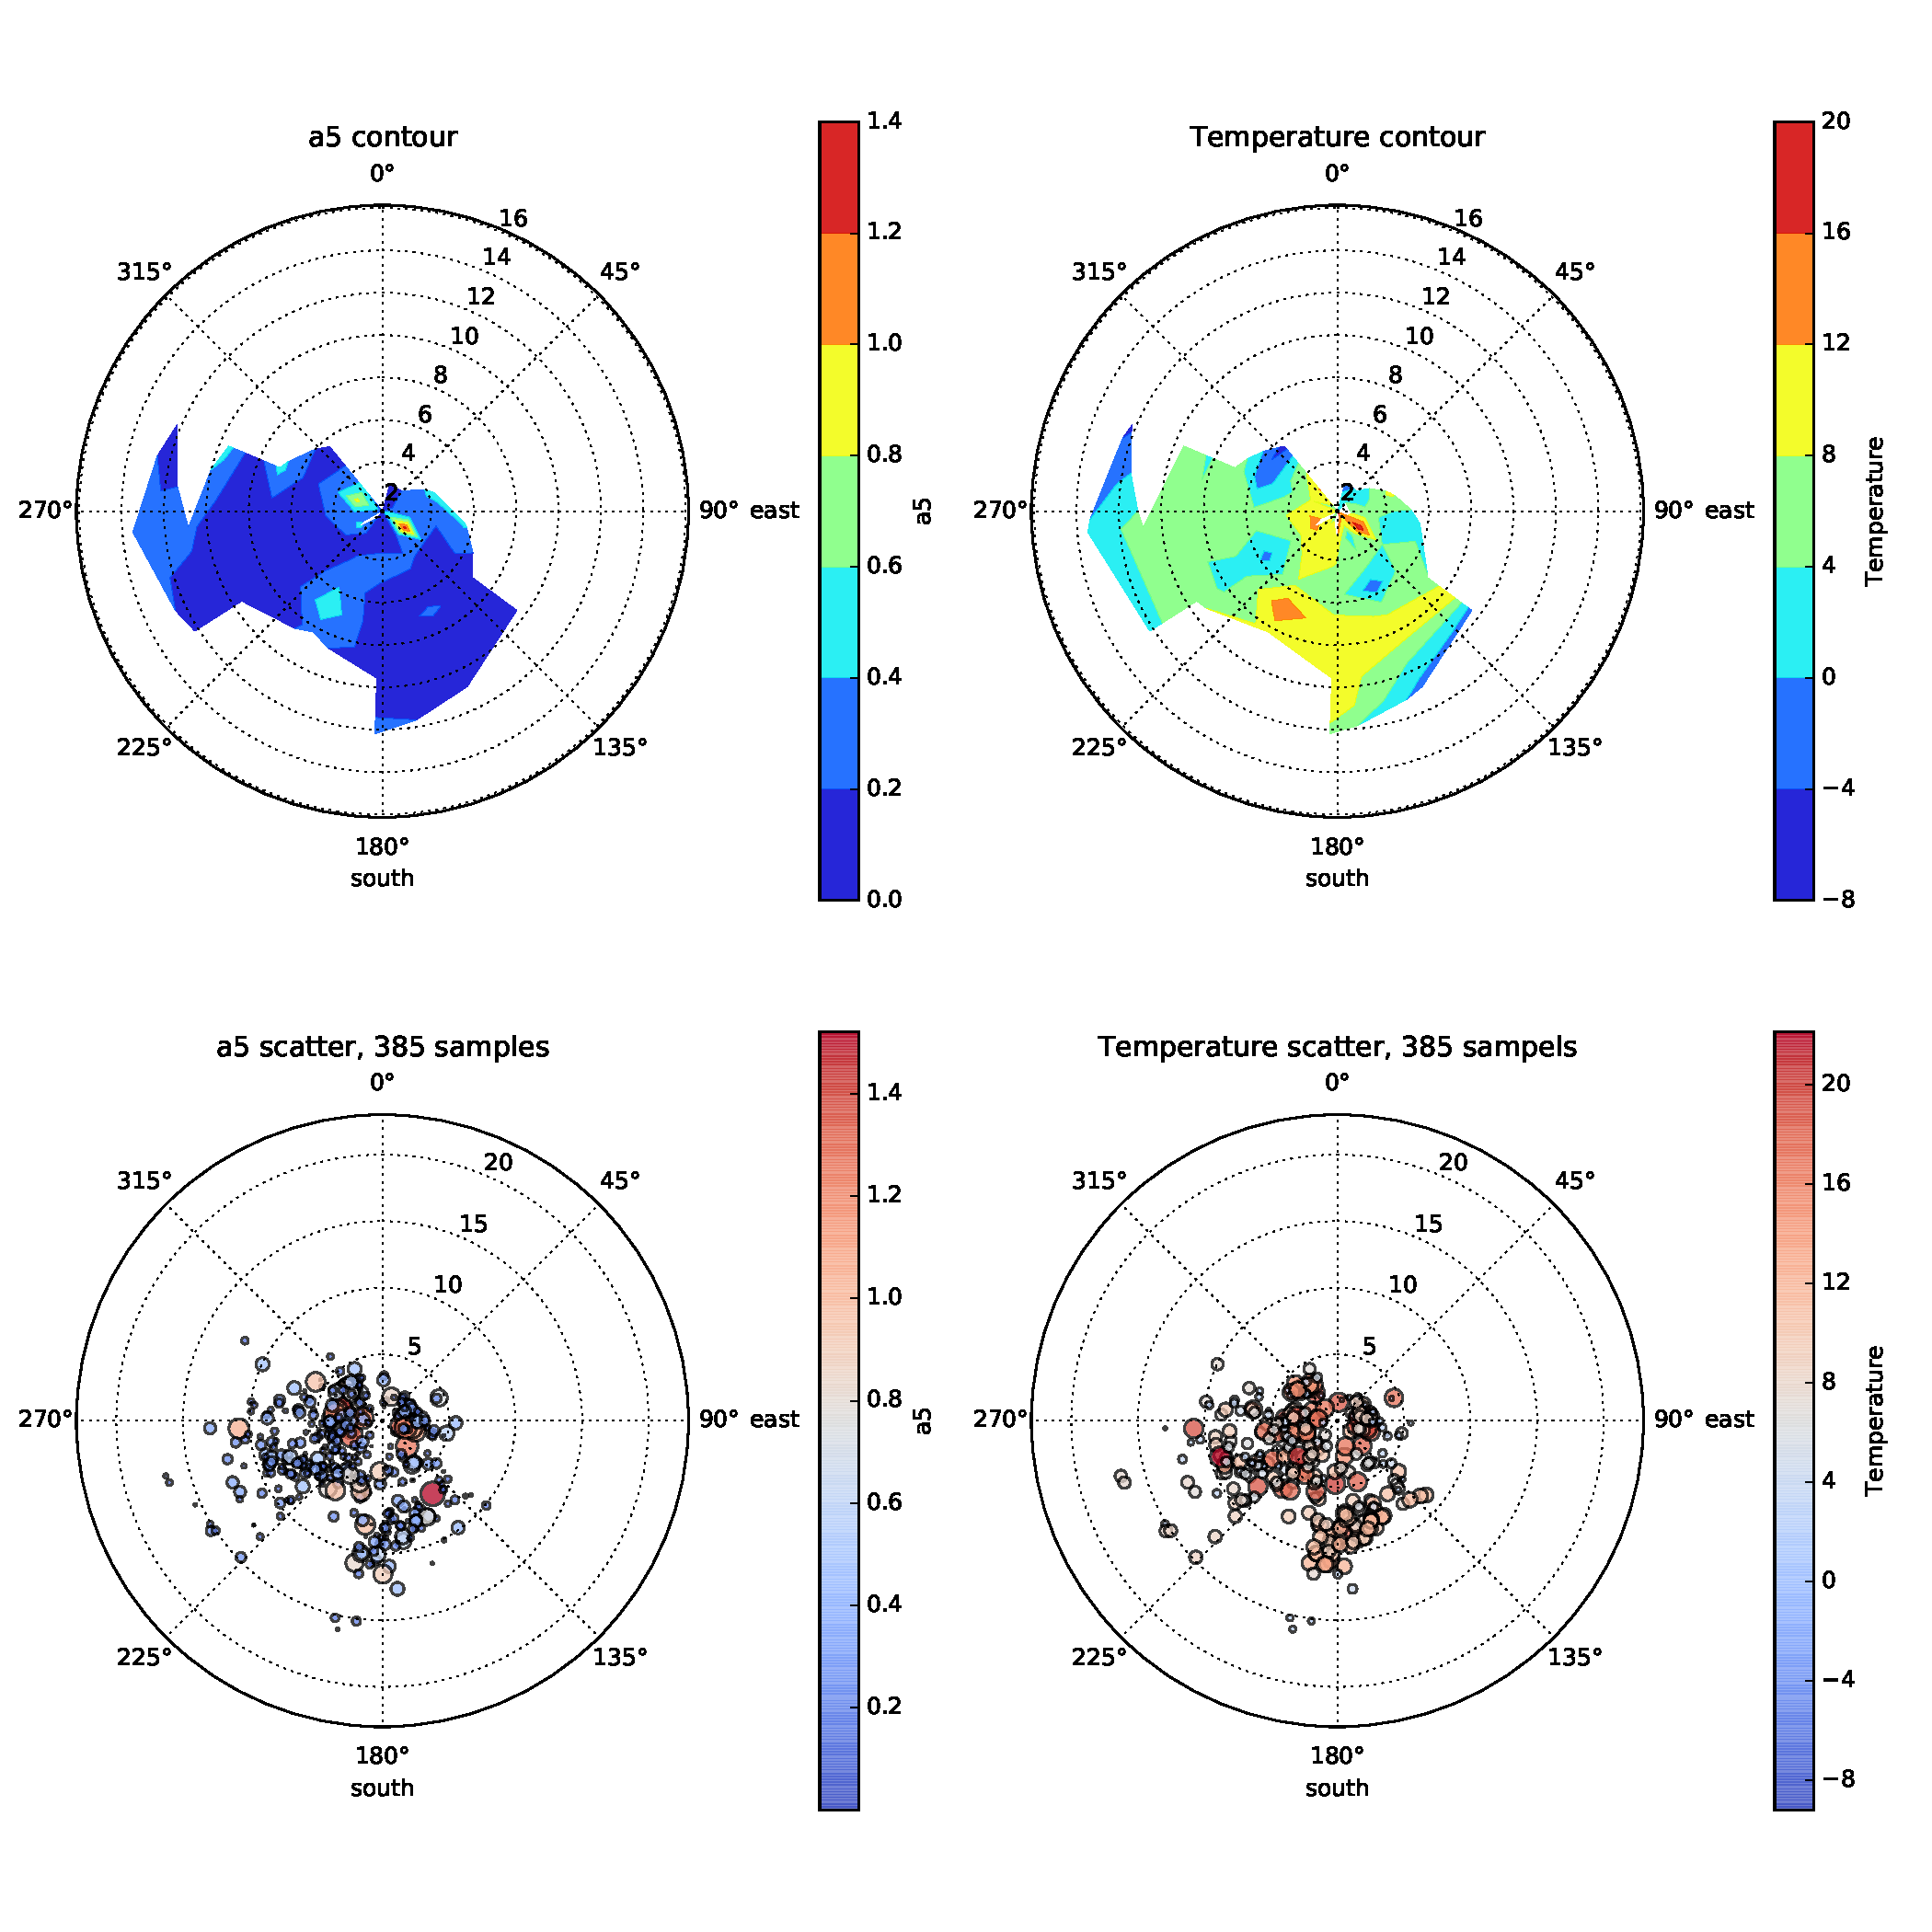
\includegraphics[scale=.46]{wind/wind_a5}
	\caption[Polarplot Windgeschwindigkeit, Windrichtung und $A_5$]{Polarplot Windgeschwindigkeit, Windrichtung und $A_5$}
    \label{wind_a5}
\end{figure}
\begin{figure}[H]
	\centering
	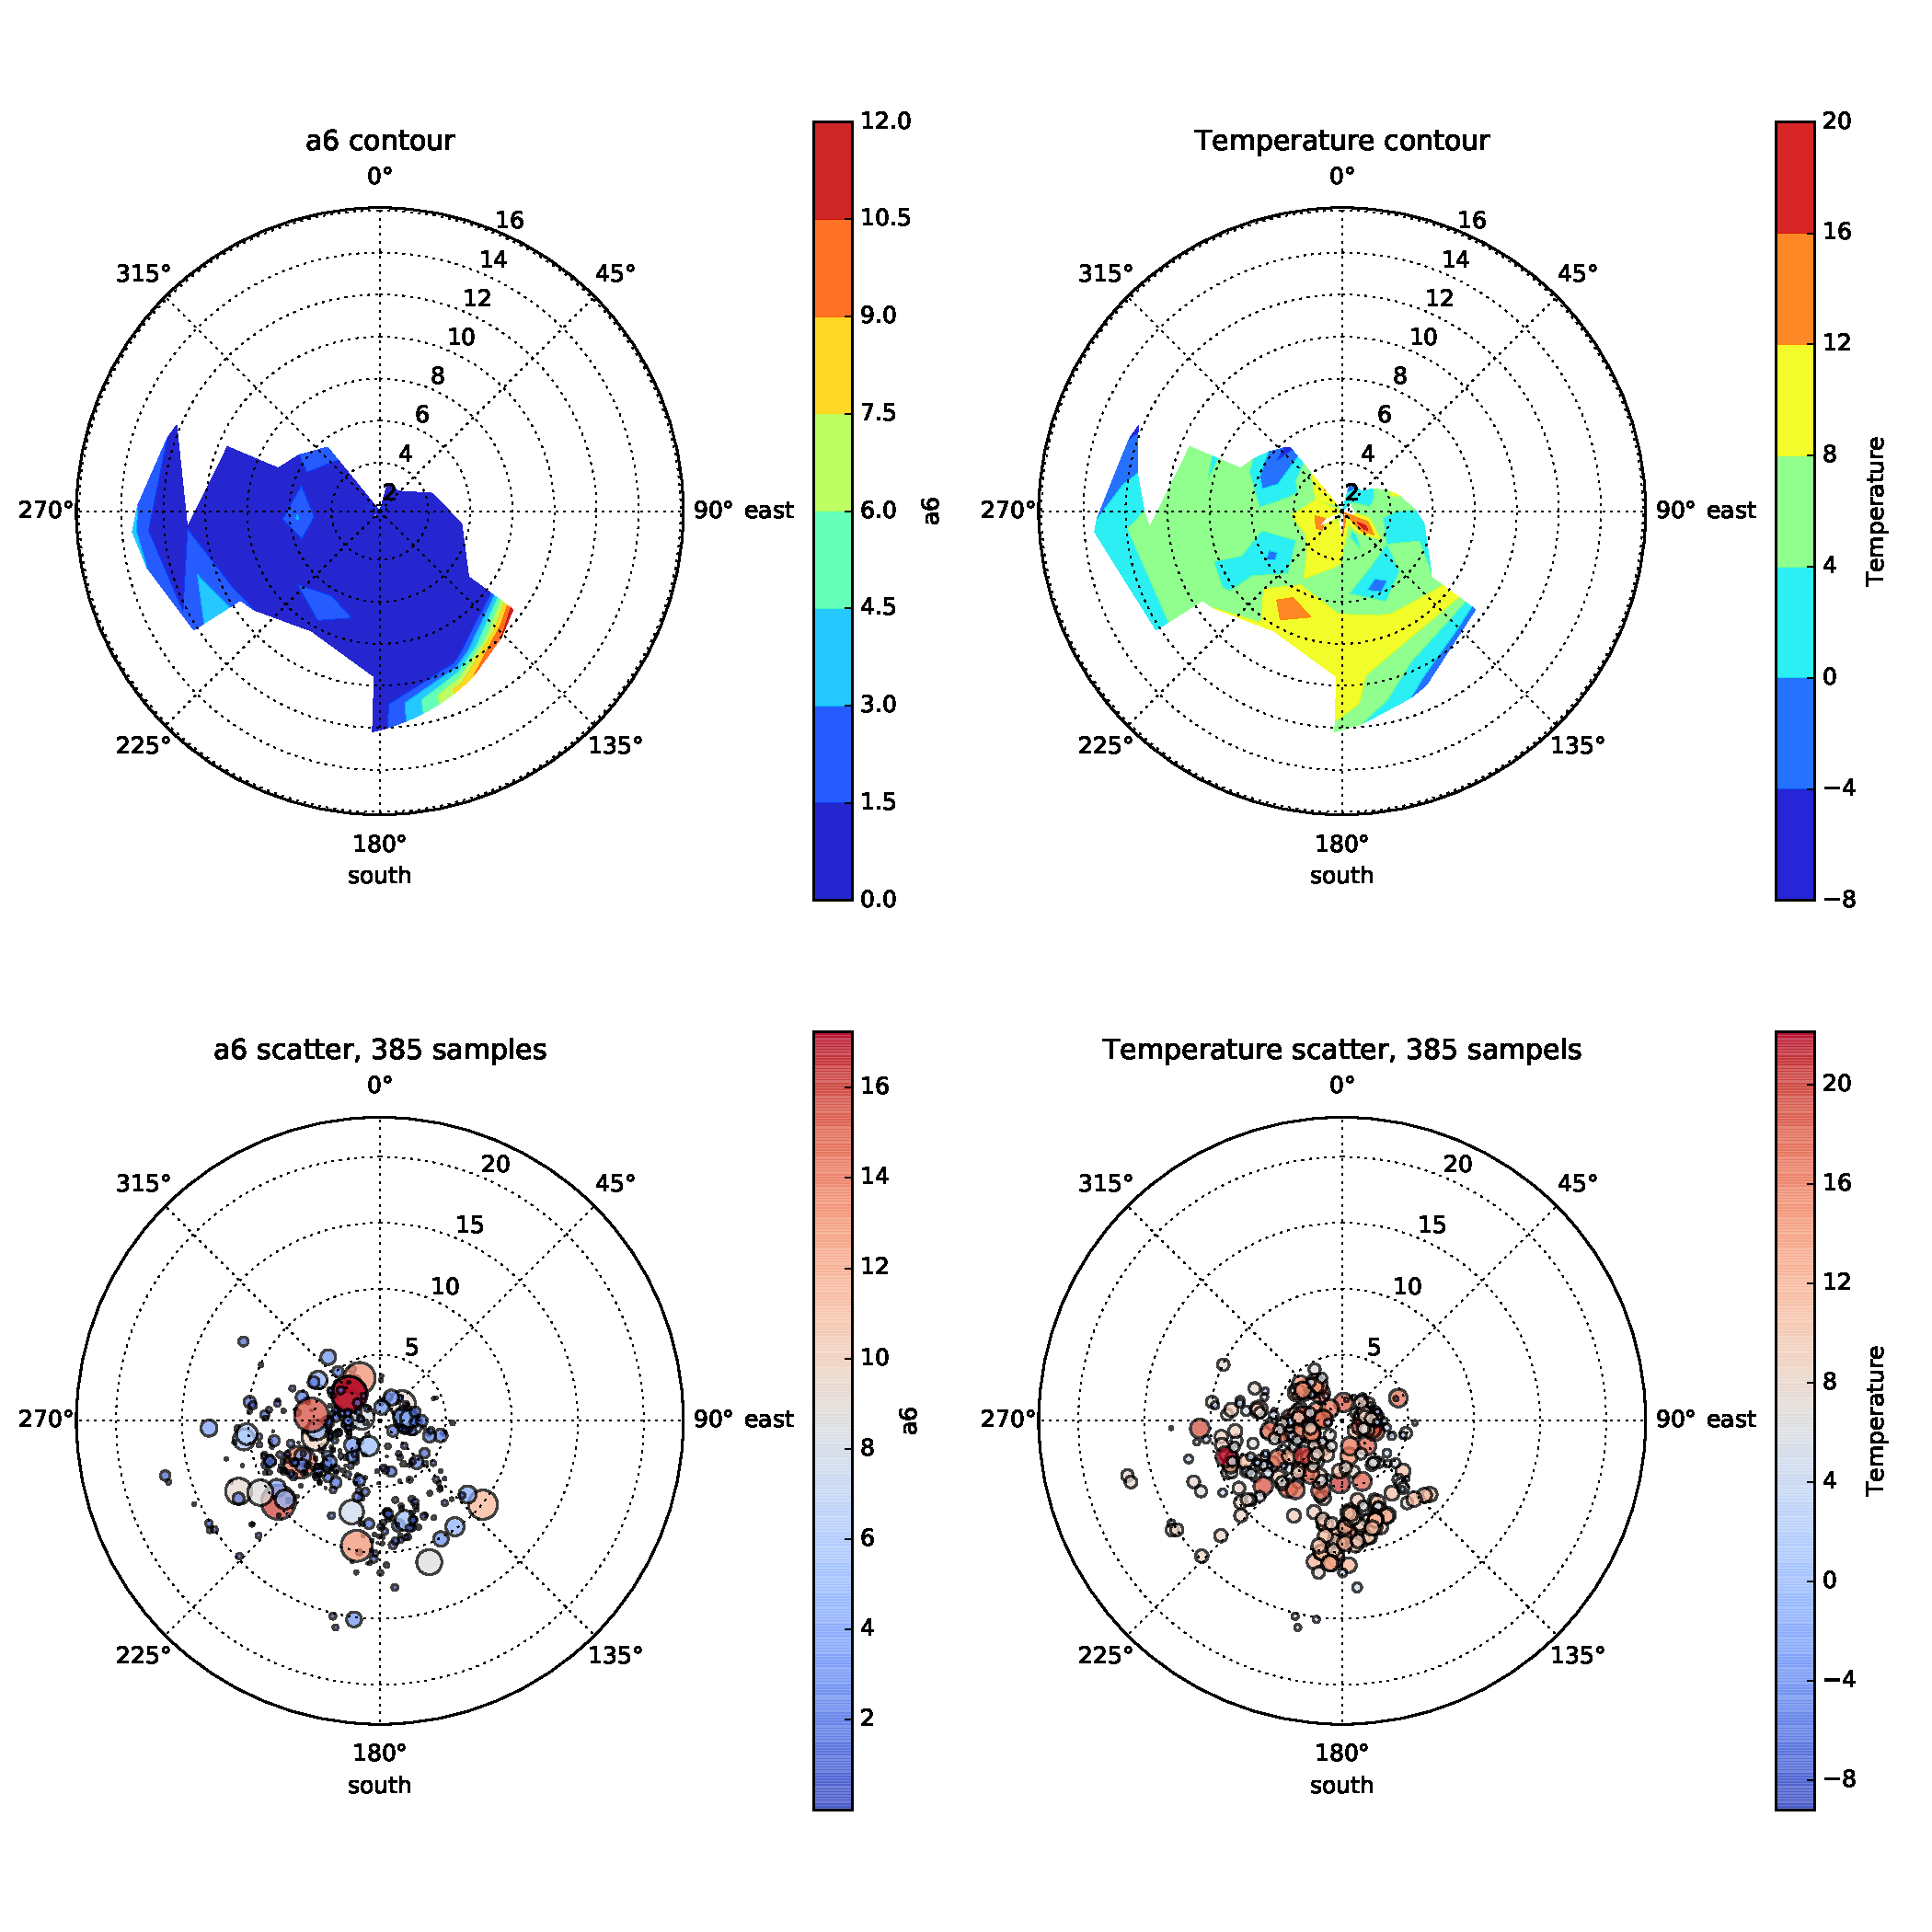
\includegraphics[scale=.46]{wind/wind_a6}
	\caption[Polarplot Windgeschwindigkeit, Windrichtung und $A_6$]{Polarplot Windgeschwindigkeit, Windrichtung und $A_6$}
    \label{wind_a6}
\end{figure}

\chapter{Quelltext}
Der komplette Quelltext ist im Softwarerepositorium zu finden.
\begin{mdframed}[style=emphasis]
	\centering
	\url{http://github.com/JeanElsner/focus-series}
\end{mdframed}
An dieser stelle soll nur Auszugsweise die Datei \emph{focus.py} aufgeführt werden, da sie das wesentliche Ergebnis dieser Arbeit darstellt. Die Datei implementiert den temperatur- und elevationsabhängigen Interpolanten der Fokusfunktion. Bildet also Temperatur und Elevation auf die Position des Sekundärspiegels entlang der optischen Achse ab.

\definecolor{mygreen}{rgb}{0,0.6,0}
\definecolor{mygray}{rgb}{0.5,0.5,0.5}
\definecolor{mymauve}{rgb}{0.58,0,0.82}

\lstset{ %
  backgroundcolor=\color{white},   % choose the background color; you must add \usepackage{color} or \usepackage{xcolor}
  basicstyle=\footnotesize,        % the size of the fonts that are used for the code
  breakatwhitespace=false,         % sets if automatic breaks should only happen at whitespace
  breaklines=true,                 % sets automatic line breaking
  captionpos=b,                    % sets the caption-position to bottom
  commentstyle=\color{mygreen},    % comment style
  deletekeywords={...},            % if you want to delete keywords from the given language
  escapeinside={\%*}{*)},          % if you want to add LaTeX within your code
  extendedchars=true,              % lets you use non-ASCII characters; for 8-bits encodings only, does not work with UTF-8
  frame=L,	                   % adds a frame around the code
  keepspaces=true,                 % keeps spaces in text, useful for keeping indentation of code (possibly needs columns=flexible)
  keywordstyle=\color{blue},       % keyword style
  language=Python,                 % the language of the code
  otherkeywords={*,...},           % if you want to add more keywords to the set
  numbers=left,                    % where to put the line-numbers; possible values are (none, left, right)
  numbersep=5pt,                   % how far the line-numbers are from the code
  numberstyle=\tiny\color{mygray}, % the style that is used for the line-numbers
  rulecolor=\color{black},         % if not set, the frame-color may be changed on line-breaks within not-black text (e.g. comments (green here))
  showspaces=false,                % show spaces everywhere adding particular underscores; it overrides 'showstringspaces'
  showstringspaces=false,          % underline spaces within strings only
  showtabs=false,                  % show tabs within strings adding particular underscores
  stepnumber=1,                    % the step between two line-numbers. If it's 1, each line will be numbered
  stringstyle=\color{mymauve},     % string literal style
  tabsize=2,	                   % sets default tabsize to 2 spaces
  title=\lstname                   % show the filename of files included with \lstinputlisting; also try caption instead of title
}

\section{focus.py}
\label{focus.py}

\lstinputlisting[language=Python]{focus.py}

\end{appendix}


  \backmatter
  \bibliographystyle{bababbrv}
\bibliography{literatur}
  \markboth{}{}

  \addcontentsline{toc}{chapter}{\protect Danksagung}


\chapter*{Danksagung}
An dieser Stelle möchte ich mich für die Unterstützung bedanken, die ich von meinem Betreuer Dr. Claus Gössl erhalten habe, der mit seiner Expertise des doch sehr komplexen Teleskop-Systems zur Verfügung stand und mir dieses Thema nähergebracht hat. Mein Dank geht auch an Dr. Ben Hoyle, der unsere regelmäßigen Treffen mit seinen informationstheoretischen Fachkenntnissen bereichert hat und mir Wegweiser zur Navigation des Python-Ökosystems aufgezeigt hat.
  
  \chapter{Selbstständigkeitserklärung}
Hiermit erkläre ich, die vorliegende Arbeit selbständig verfasst zu haben und keine anderen als die in der Arbeit angegebenen Quellen und Hilfsmittel benutzt zu haben.

  \vspace{1em}
  \noindent
  \begin{tabular}{cc}
  	\; & \; \\
  	\makebox[2.5in]{\hrulefill} & \makebox[2.5in]{\hrulefill}\\
  	Unterschrift & Ort, Datum\\
  \end{tabular}

\end{document}
